\documentclass[twoside]{book}

% Packages required by doxygen
\usepackage{calc}
\usepackage{doxygen}
\usepackage{graphicx}
\usepackage[utf8]{inputenc}
\usepackage{makeidx}
\usepackage{multicol}
\usepackage{multirow}
\usepackage{textcomp}
\usepackage[table]{xcolor}

% Font selection
\usepackage[T1]{fontenc}
\usepackage{mathptmx}
\usepackage[scaled=.90]{helvet}
\usepackage{courier}
\usepackage{amssymb}
\usepackage{sectsty}
\renewcommand{\familydefault}{\sfdefault}
\allsectionsfont{%
  \fontseries{bc}\selectfont%
  \color{darkgray}%
}
\renewcommand{\DoxyLabelFont}{%
  \fontseries{bc}\selectfont%
  \color{darkgray}%
}

% Page & text layout
\usepackage{geometry}
\geometry{%
  a4paper,%
  top=2.5cm,%
  bottom=2.5cm,%
  left=2.5cm,%
  right=2.5cm%
}
\tolerance=750
\hfuzz=15pt
\hbadness=750
\setlength{\emergencystretch}{15pt}
\setlength{\parindent}{0cm}
\setlength{\parskip}{0.2cm}
\makeatletter
\renewcommand{\paragraph}{%
  \@startsection{paragraph}{4}{0ex}{-1.0ex}{1.0ex}{%
    \normalfont\normalsize\bfseries\SS@parafont%
  }%
}
\renewcommand{\subparagraph}{%
  \@startsection{subparagraph}{5}{0ex}{-1.0ex}{1.0ex}{%
    \normalfont\normalsize\bfseries\SS@subparafont%
  }%
}
\makeatother

% Headers & footers
\usepackage{fancyhdr}
\pagestyle{fancyplain}
\fancyhead[LE]{\fancyplain{}{\bfseries\thepage}}
\fancyhead[CE]{\fancyplain{}{}}
\fancyhead[RE]{\fancyplain{}{\bfseries\leftmark}}
\fancyhead[LO]{\fancyplain{}{\bfseries\rightmark}}
\fancyhead[CO]{\fancyplain{}{}}
\fancyhead[RO]{\fancyplain{}{\bfseries\thepage}}
\fancyfoot[LE]{\fancyplain{}{}}
\fancyfoot[CE]{\fancyplain{}{}}
\fancyfoot[RE]{\fancyplain{}{\bfseries\scriptsize Generated on Sat May 9 2015 00\-:55\-:45 for Cuda S\-P\-H Fluid Simulation -\/ Declan Russell by Doxygen }}
\fancyfoot[LO]{\fancyplain{}{\bfseries\scriptsize Generated on Sat May 9 2015 00\-:55\-:45 for Cuda S\-P\-H Fluid Simulation -\/ Declan Russell by Doxygen }}
\fancyfoot[CO]{\fancyplain{}{}}
\fancyfoot[RO]{\fancyplain{}{}}
\renewcommand{\footrulewidth}{0.4pt}
\renewcommand{\chaptermark}[1]{%
  \markboth{#1}{}%
}
\renewcommand{\sectionmark}[1]{%
  \markright{\thesection\ #1}%
}

% Indices & bibliography
\usepackage{natbib}
\usepackage[titles]{tocloft}
\setcounter{tocdepth}{3}
\setcounter{secnumdepth}{5}
\makeindex

% Hyperlinks (required, but should be loaded last)
\usepackage{ifpdf}
\ifpdf
  \usepackage[pdftex,pagebackref=true]{hyperref}
\else
  \usepackage[ps2pdf,pagebackref=true]{hyperref}
\fi
\hypersetup{%
  colorlinks=true,%
  linkcolor=blue,%
  citecolor=blue,%
  unicode%
}

% Custom commands
\newcommand{\clearemptydoublepage}{%
  \newpage{\pagestyle{empty}\cleardoublepage}%
}


%===== C O N T E N T S =====

\begin{document}

% Titlepage & ToC
\hypersetup{pageanchor=false}
\pagenumbering{roman}
\begin{titlepage}
\vspace*{7cm}
\begin{center}%
{\Large Cuda S\-P\-H Fluid Simulation -\/ Declan Russell \\[1ex]\large 1.\-0 }\\
\vspace*{1cm}
{\large Generated by Doxygen 1.8.6}\\
\vspace*{0.5cm}
{\small Sat May 9 2015 00:55:45}\\
\end{center}
\end{titlepage}
\clearemptydoublepage
\tableofcontents
\clearemptydoublepage
\pagenumbering{arabic}
\hypersetup{pageanchor=true}

%--- Begin generated contents ---
\chapter{Main Page}
\label{index}\hypertarget{index}{}\section*{Cuda Smoothed Particle Hydrodynamics Report }

 \section*{Introduction }

The contents of this report follows the design and implimentation of a real time fluid simulation. This implimentation takes the form of a 3\-D Langrangian grid and takes advanteges of the speed of Nvidia's Cuda A\-P\-I to create a fast realistic fluid simulation. In the following sections you will find an explenation of maths used, optimisations made and the implimentation of this artifact.

\section*{Smoothed Particle Hydrodynamics and Fluid Theory }

When implimenting fluid simulations there is an array of techniques in which you can use. Each of which have there own advantages and disadvanteges. The most prominent of these techniques are Eulerian and Langrangian.
\begin{DoxyItemize}
\item Eulerian Method Looks at fluid motion through specific locations in space. Space is devided up into cells which store attributes about the fluid in that location such as pressure, velocity and desity etc...
\begin{DoxyItemize}
\item Advanteges
\begin{DoxyItemize}
\item Performance determined by grid size not number of particles
\item Fast
\end{DoxyItemize}
\item Disadvanteges
\begin{DoxyItemize}
\item Detail contrained to grid size
\item Simulation size limited to grid size
\end{DoxyItemize}
\end{DoxyItemize}
\item Langrangian Method Focuses on individual particles of the fluid. Each particle stores attributes about its own pressure, velocity and density.
\begin{DoxyItemize}
\item Advanteges
\begin{DoxyItemize}
\item Simulation size not limited.
\end{DoxyItemize}
\item Disadvanteges
\begin{DoxyItemize}
\item Performance tied to number of particles
\item For a realistic simulation we need to have a lot of particles
\end{DoxyItemize}
\end{DoxyItemize}
\end{DoxyItemize}

For this implimentation I will be following the Langrangian method.

\subsection*{Navier Stokes Equations }

Navier stokes equations mathematically model the behaviour of fluid. The they look at calculating forces apparent in the fluid and give us an acceleration with from the sum all these forces. below is the Langrangian fluid equation for weakly compressible flow.\par
 \[ \rho\frac{du}{dt}=-\bigtriangledown\rho+\mu\bigtriangledown^2 u + f \]\par
 On the left of this equation you will see the greek symbol $\rho$ which stands for the density of the of the fluid. This is multiplied by $\frac{du}{dt}$ which is the excelleration of our particle at the next timestep. Now lets break down the three componts on the right hand side of the equation.\par
 \[ -\bigtriangledown\rho \]\par
 This term represents the gradient of pressure of our particle. Giving the direction that the pressure is in and the magnitude of this pressure\par
 \[ \mu\bigtriangledown^2 u \]\par
This term represents the viscosity force acting upon our particle. $\mu$ Being a scaler coefficient that can be set by the user to increase of decrease the viscosity force acting upon our fluid.\par
 \[ f \]\par
Our third and final term in this formulae represents any external forces acting upon our fluid. This could be anything from gravity, suface tension or any other forces you may need to interact with our fluid.

\subsection*{Smoothed Particle Hydrodynamics }

Smoothed particle hydrodynamics is a technique that provides a collection of approximation formulae to solve our Navier Stokes equations. It focuses on scaling the forces in our Navier Stokes equation based on the distance between particles. Closer particles will have a much higher influence on our forces than particles further away. To do this we will specify a wighting kernel which I will specify later.

\subsection*{Calculating our forces }

\subsection*{Density }

As you can see from our Navier Stokes equations every force must be devided by the particles density to calculate the acceleration therefore the first force we must calculate must be the density of our particles. To do this we use the formulae below.\par
 \[ \rho(x_i)= \sum\limits_{j}m_j W_{default}(x_i-x_j,h) \]\par
 This formulae represents the sum of $m$ which is the mass of our neightbouring particle. In our simluation our mass will be a constant with all particles having the same mass. This is then multiplied by function $W$ which is our weighting kernel. More on how we calculate that later.

\subsection*{Pressure Gradient }

Once we have our the densities of our particles calulated we can now move on to computing our pressure gradient. To do this firstly however we must calculate the pressure per particle in our simulation. This is computed with the following equation,\par
 \[ p_i = k(\rho_i - \rho_0) \]\par
 Here we have variable $k$ which is the gas constant of our fluid and will be set by the user depending on their desired fluid behaviour. $\rho_i$ is the density of the particle that we are calcuating the pressure for and $\rho_0$ is the rest density of our fluid. This is also a constant that the use will set by the user depending on their desired fluid behaviour. Now that we have our pressure per particle, we can use this to to compute our pressure gradient function,\par
 \[ f_i^{pressure} = -\sum\limits_{i\neq j}p_j\frac{m_j}{\rho_j}\bigtriangledown W_{pressure}(x_i-x_j,h) \]\par
The formulae above represents the summation of particle properties $j$ when $j$ is not equal to $i$. The variable $m_j$ is our particle mass, $\rho_j$ is the density of our particle which we calculated using the equation in the previous section and $W$ is our pressure weighting kernel which I will discuss later. However there is a problem when using this equation. The pressure force calculated is not symetrical as particle $i$ only uses the the pressure at particle $j$ to compute the pressure gradient. This problem can be solved however by using an different proposed equation \mbox{[}M\-J92\mbox{]}, \[ f_i^{pressure} = -\sum\limits_{i\neq j}(\frac{p_i}{\rho_i^2} + \frac{p_j}{\rho_j^2})m_j\bigtriangledown W_{pressure}(x_i-x_j,h) \]

\subsection*{Viscosity Force }

Next we can calculate our viscosity force, the larger this force is the more it gives the fluid a thicker or stickier appearence. An example of a very viscous fluid would be syrup. To calculate this force we use the following equation, \[ f_i^{viscosity} = \mu\sum\limits_{i\neq j}(u_j-u_i)\bigtriangledown^2 W_{viscosity}(x_i-x_j,h) \]\par
In this equation we have one more unknown $\mu$, this represents the viscosity force. This is a scaler value set by the user to for the desired visocity influence on the fluid. Also you may notice that this formulae also contains a third weighting kernel which will be explained in the next section.

\subsection*{Velocity Correction }

A problem with our fluid is it can succumb to compression which will cause very high areas of density ultimately leading to our particles acting quite violently. One method to counter this is know as X\-S\-P\-H \mbox{[}P\-A09\mbox{]} which averages the velocity of our particles with its neighbours improving its overall flow. \[ v_i = v_i + \epsilon\sum\limits_j\frac{2m_j}{\rho_i+\rho_j}(v_j-v_i)W_{default}(x_i-x_j,h) \] Where $\epsilon$ is a scaler value of how much correction we want to apply to our particle. Its important to note however we do not want this to be too high as it will ruin the physical correctness of our simulation.

\subsection*{Other forces }

Finally our final unknown is $f$. For this implimentation $f$ will only represent gravity which we will assume is a constant 9.\-8m/s in the negative y direction. However for future work this can be extented to also include any other forces you may want to include such as surface tension or some kind of interaction forces.

\subsection*{Weighting kernels }

As mentioned in the previous sections all our force equations use a weighting kernel which scales the force value calculated based on the distance particles are from each other. The first of these kernels we encountered was the function $W_{default}$ which can be denoted,\par
 \[ \newcommand{\twopartdef}[4] { \left\{ \begin{array}{ll} #1 & \mbox{if } #2 \\ #3 & \mbox{if } #4 \end{array} \right. } W_{default}(r,h) = \frac{315}{64\pi h^9}\twopartdef{(h^2-||r||^2)^3}{0\leq ||r|| <h}{0}{||r||>h} \]

In this equation $r$ is equivilent to vector from our neighbour particle to our current particle. The letter $h$ is the smoothing length of our equation. This variable is set before the simulation is run and will affect the behaviour of our fluid.\par
The above weighting kernel will look like this when assuming that the soomthing length is 1,\par
 This smoothing kernel is sutible for use on our density calculations but however will not be suitible for when we calculate our pressure. This is due to the gradient of the function tending to 0 as the distance of our particles tends to 0. To use this weighting kernel would create clustering of our particles. Ideally we would want our pressure kernel to continually get larger as our distance approaches 0 and is at the point of highest pressure. This is solved in \mbox{[}M\-M03\mbox{]} with their proposed \char`\"{}\-Spikey\char`\"{} kernel. \[ W_{pressure}(r,h) = W_{spikey}(r,h) = -\frac{45}{\pi h^6} \frac{r}{||r||}(h-||r||)^2 \]

Again assuming that our smoothing length $h$ is 1 our smoothing kernel will look like,\par
 Notice how our kernel now tends to infinity due to our division of the length of $r$ solving our clustering problem.

Our final weighting kernel is for our viscosity term. Also proposed \mbox{[}M\-M03\mbox{]} is the following kernel,\par
 \[ W_{viscosity}(r,h) = -\frac{45}{\pi h^6}r(h-||r||) \] If is important to note that unlike the pressure weighting kernel, the values from our viscosity weighing are always positive. This is because the viscosity term acts as a damping force, if values were to become negative it would increase the energy of our particles.\par
Again assuming that our smoothing length $h$ is 1 our smoothing kernel will look like,\par
 \subsection*{Integration Methods }

\subsection*{Euler }

To update our particles position we must integrate our acceleration to calculate first our velocity and then our displacement. The most basic integration we can use is Euler integration which goes as follows,\par
 \[ u = u + adt \] \[ x = x + udt \]

We have four unknowns in these equations. $x$, $u$ and $a$ are our position, velocity and acceleration. Our final unknown $dt$ is the timestep of our update. However the problem with this method is that as the simulation the chance of error when using these equations increases over time. These means the longer the simulation is running for the more inaccurate and unstable it will get. \subsection*{Leap Frog }

A more stable method to use is the Leap Frog method. This method uses future half step velocity and a previous half step velocity to calculate the position at the next half time step. This method proves much more stable than our Euler method. It is achieved with the equations below,\par
 \[ u_{t+\frac{1}{2} \triangle t} = u_{t- \frac{1}{2} \triangle t} + \triangle t a_t \] \[ u_{t-\frac{1}{2} \triangle t} = u_0 - \frac{1}{2}\triangle t a_0 \] \[ x_{t+\frac{1}{2} \triangle t} = x_t - \triangle tu_{t+\frac{1}{2} \triangle t} \] Below is a graph comparing the error of Leap Frog compared to other popular integration techniques over time with a deliberately high timestep used.\par
As you can see from the graph although the accuracy may drop the integration technique stays very stable over long periods of time.

\section*{Optimisations }

\subsection*{Spacial Hash }

When sampling neighbouring particles it it computationally inificient to sample all the particles in our scene. If every particle $n$ samples every orther particle $n$ then we reach an overall computational complexity of $O(n^2)$ which means our simulation will get exponetially slower the more particles we simulate in our scene. Any particles outside our smoothing length are given an influence of 0 on our particle, this means we can exclude them from our calculations. Idealy we want to only sample a set number of particles within our smoothing length which we can accomplish this with the use of a spacial hash. This spacial hash will assign particles that are near each other a unique key. we can then use this key to identify the particles that we need to sample. If we choose the maximum number of particles to sample and keep that as a constant value this reduces our complexity to $O(n)$ which is fast. For this implimentation I have used a very simple hash function,\par
 \[ p_n = p/s_g \] \[ r = s_g/h \] \[ p_g = \lfloor p_n*r \rfloor \] \[ idx = p_{gx}*r^2 + p_{gy}*r +p_{gz} \] Where $p$ is our position, $s_g$ is the dimention size of our hash grid and $h$ is our smoothing length. $r$ refers to the resolution of our grid. We compute it this way so that every cell in our hash is the size of our smoothing length and particles of this cell and neighbouring cells are likely to be within our smoothing length. This is visualised in the image below.\par
As you can see from the image above, neighbouring cells particles must be taken into account in our samples as they may still lie within the smoothing length of our particle. Finding neighbouring hash keys is fast though and can be computed in the following way,\par
 \[ neighbour idx = idx + (dx*r^2 + dy*r + dz) \] Where $dx,dy$ and $dz$ are the offset of the neighbour hash cell we desire.

\subsection*{C\-U\-D\-A }

C\-U\-D\-A or Compute Unified Device Architecture is a parallel computing A\-P\-I create from Nvidia which allows you to take control of your G\-P\-U's parallel architecture. This is ideal for our fluid simulation as it gives us the ability to process all our particle calculations at the same time rather than if we were to do this on the C\-P\-U in serial. This gives us the ability to simulate a much larger number of particles in our simulation. In the following sections I will discuss the implimentation of this.

\subsection*{C\-U\-D\-A implimentation }

Important things to take into account when programming on the G\-P\-U.\par

\begin{DoxyItemize}
\item Copying from G\-P\-U to C\-P\-U is slow, preferably we want to keep everything on the G\-P\-U as much as possible.
\item Accessing global memory from the G\-P\-U is slow, we should keep this to a minumum as much as possible. \par
First of all we need to set up some buffers to make our implimentation posible. The buffers needed are
\item Position buffer, size of how many particles we have.
\item Velocity buffer, size of how many particles we have.
\item Hash key buffer, size of how many particles we have.
\item Cell Occupancy buffer, size of our hash table. This can be calculated from the resolution cubed.
\item Cell Index buffer, size of our hash table. \par

\end{DoxyItemize}
\begin{DoxyEnumerate}
\item Hashing partilces\par
 The first thing we need to do is hash our particles to give them a key based on their position. To do this we assign a thread to for everyparticle. Now simply use the equation from the previous section to out put our hash keys into a new buffer.
\item Sort our particle data by hash key.\par
 This is important to reduce banking conflicts when accessing from the global memory of our G\-P\-U. Global memory copies are slow so we want to do as little of them as possible. When you tell a cuda kernal to access global memory the bus will also give you the data from contiguous memory locations aswell. So for speed improvements we need to keep our memory as contiguous as possible reducing the number of global memory copies we do. To achieve this sort we can simply use thrust, a library of prewritten cuda functions. Thrust has its own sort\-\_\-by\-\_\-key function which is perfectly suitible for our needs.
\item Count Cell Occupancy\par
 We need to know the cell occupancy to know how many particles are in each cell. This also helps use identify where our particles are stored in memory. To count the cell occupancy is fairly simple. We assign a thread for every entry in our hash key buffer and we increment the value in our Cell Occupancy buffer relative to this hash key. However it is important to know that to avoid race conditions between threads. To solve this we can use C\-U\-D\-A's atomic add function to do this. This uses a mutex to lock the memory address while it is being modified by the current thread.
\item Create our cell index buffer\par
 This will give us the particle index of particles that belong in our cell. To compute this we can just create a running total of all the entries in our cell occupancy buffer. Thrust can again be used as its exlusive\-\_\-scan function does just this in paralell.
\item Fluid Solving Now we have all our buffers prepared we can use our navier stokes equations and solve for our new particle position.
\begin{DoxyEnumerate}
\item Assign a block of threads to every cell in our hash table.
\item Load our neighbouring particle data into shared memory.\par
 As we need to access neighbour particle data a lot in our calculations accessing global memory multiple times is going to add a lot of overhead to our solver. In the G\-P\-U architecture however every block has its own shared memory which can be accessed by all threads in that block. This shared memory is considerably faster than accessing global memory. Therefore its more efficient for us to copy once from global memory into shared memory than continuously copy from global memory.
\item Assign every thread a particle.
\item Perform our calculations on each particle
\item Update particle positions
\end{DoxyEnumerate}
\item Collision detection\par
 The collision detection in this implimentation is very simple. I simply assign every particle to a thread and perform A\-A\-B\-B collision detection on every position. If it has collided with the collision object the position is simply pushed back and the velocity of the particle is flipped.
\end{DoxyEnumerate}

\subsection*{Reducing some arithmetic computation }

Threads on the G\-P\-U do not have as much arithmetic power when compared to the C\-P\-U. This means that arithmetic operations that we perfrom on the G\-P\-U will have an impact on overhead on each kernal launch. To improve this we want to limit the number of operations as much as we can. A good example of this is our weighting kernals, \[ \newcommand{\twopartdef}[4] { \left\{ \begin{array}{ll} #1 & \mbox{if } #2 \\ #3 & \mbox{if } #4 \end{array} \right. } W_{default}(r,h) = \frac{315}{64\pi h^9}\twopartdef{(h^2-||r||^2)^3}{0\leq ||r|| <h}{0}{||r||>h} \] Notice that during our simulation assuming that we dont regularly change our smoothing length then $\frac{315}{64\pi h^9}$ will remain constant. It actually become more efficient if we precalculate this on the C\-P\-U and load it in as a paramiter to our C\-U\-D\-A kernal. We can see another example in our pressure kernal,\par
 \[ f_i^{pressure} = -\sum\limits_{i\neq j}(\frac{p_i}{\rho_i^2} + \frac{p_j}{\rho_j^2})m_j\bigtriangledown W_{pressure}(x_i-x_j,h) \] Throughout our sum loop $\frac{p_i}{\rho_i^2}$ will be the same. Instead of recomputing this every loop we can just compute it once, store the value and use it when needed. Secondly our mass $m_j$ is constant, this means we can move it out side our loop reducing our multiply operations to just 1 time rather than $j$ times. Our final equation will look like this, \[ p1 = \frac{p_i}{\rho_i^2} \] \[ f_i^{pressure} = -m_j\sum\limits_{i\neq j}(p1 + \frac{p_j}{\rho_j^2})\bigtriangledown W_{pressure}(x_i-x_j,h) \] Simplifications like this can be made to all our equations. \subsection*{C\-U\-D\-A Streams and Multiple Simulations }

Another optimisation that C\-U\-D\-A provides are streams. This allows you to launch C\-U\-D\-A operations with a chance of operations in different streams being run concurrently. For this implimentation I have used this when creating seperate fluid simulations at the same time. This technique could be explored in further research to improve on how we launch the kernals to update our fluid simulation. More information about C\-U\-D\-A streams here\-: \href{http://on-demand.gputechconf.com/gtc-express/2011/presentations/StreamsAndConcurrencyWebinar.pdf}{\tt http\-://on-\/demand.\-gputechconf.\-com/gtc-\/express/2011/presentations/\-Streams\-And\-Concurrency\-Webinar.\-pdf} \subsection*{Simulation Performance }

Below you can see a graph representing the simulation performance when simulating different quantities of particles. 

\section*{Rendering }

The rendering technique of this simulation is taken from \mbox{[}G\-S10\mbox{]} and provides an efficient way of rendering particles as an implicit surface without the need for any descrete geomtry or polygonization techniques. In this section I will discuss how it is achieved,


\begin{DoxyEnumerate}
\item Rendering Particle Spheres\par
 It is possible to render point sprites as spheres. For detail about how this is done please refer to my particle\-Depth shader. To do this is very cheap and is possible to render millions of spheres without any framerate drop. When compared to instanced descrete spheres the performance is not even close.
\item Render Depth Pass of Particles\par
 The first pass of our shader will be to render our particle spheres as a depth parse to a render target. It should look something like this,\par
 
\item Bilateral filter\par
 Now we blur the depth pass to create a smooth surface to our render. It is important to note that the type of blur you choose to do this will makes a big difference to the final render. The Bilateral Filter (see implimentation for more details) takes depth into account when blurring so that particles in the foreground are not blended into the background. We also render this pass to a render target and should look something like this,\par
 
\item Calculate Normals\par
 From this blured depth pass we can calculate the normals by converting from screen position and depth values to world space. We can then use partial derivatives to produce the normal at the position in eyespace. See below,\par
 
\item Thickness\par
 We can generate a thickness pass by rendering our particle spheres with additive blending and no depth test. This will mean that particles will render on top of each other. When particles are rendered on top of each other the values are accumilated thus giving us higher color values in bigger densities.\par
 
\item Final Shading For our final shading I do simple cube map reflection and refraction on our surface using the eyespace normal. You then blend your disired water colour with the refraction colour based on value from our thickness pass.\par
    
\end{DoxyEnumerate}

\section*{Some Design Choices }

The initial design for my main program is very basic. Firstly I have one class to manage the fluid simulation, essentially a class of accesors and mutators that calls our cuda kernals which do all the work. Secondly a class to manage our fluid shading. Keeping this as its own class means that It can be easily ported to another program if needs be. And finally our open\-G\-L context class which manages our cameral controls.\par
 However when creating my shader class I realised that It required a lot of open\-G\-L texture and render target managment. In the desire to create cleaner code I have created library classes for each of these to support my shader class and make managment of these objects easier. These library classes are both singleton classes so that you may access them when and where you need to. The purpose of these classes are to create and store the relative open\-G\-L objects allowing you to easily access them when desired. See below the design of these classes.\par


\section*{References }

\mbox{[}P\-A09\mbox{]} Paiva, A., Petronetto, F., Lewiner, T. and Tavares, G. (2009). Particle-\/based viscoplastic fluid/solid simulation\par
\mbox{[}M\-J92\mbox{]} Monaghan, J. (1992). Smoothed particle hydrodynamics, Annual Review of Astronomy and Astrophysics, pp. 543–574.\par
\mbox{[}M\-M03\mbox{]} Muller, M., Charypar, D. and Gross, M. (2003). Particle-\/based fluid simulation for interactive applications, S\-C\-A ’03\-: Proceedings of the 2003 A\-C\-M S\-I\-G\-G\-R\-A\-P\-H\par
\mbox{[}G\-S10\mbox{]} Green, S., 2010 Screen Space Fluid Rendering for Games., \href{http://developer.download.nvidia.com/presentations/2010/gdc/Direct3D_Effects.pdf}{\tt http\-://developer.\-download.\-nvidia.\-com/presentations/2010/gdc/\-Direct3\-D\-\_\-\-Effects.\-pdf}\par

\chapter{A\-G\-S\-D\-T\-Fluid\-Sim}
\label{md__home_dexternation__a_g_s_d_t_fluid_sim__r_e_a_d_m_e}
\hypertarget{md__home_dexternation__a_g_s_d_t_fluid_sim__r_e_a_d_m_e}{}
A fluid simulation for my advanced graphics software development techniques unit. This is an S\-P\-H Fluid simulation that uses dynamic parallelism and fancy shading techniques.

Instalation and running\-:

For this simulation to run your G\-P\-U will need the to have compatibility with cuda and dynamic Parallelism. This will require an N\-Vidia chip of compute caperbility 3.\-5 or higher! It should work on both mac and linux but I have not tested for mac so don't hold me to this!

Step 1\-: You will need to tweak your gencode caperbility in the .pro file to your hardware configuration. Step 2\-: (optional) Depending on what version on cuda you are running you may have to change the path to your cuda library in the .pro aswell. Im running 6.\-5 so if you are the same you should be fine. Step 3\-: In the A\-G\-S\-D\-T\-Fluid\-Sim directory run, \begin{DoxyVerb}qmake
make clean
make
\end{DoxyVerb}


step 4\-: You should now have a working executable. Please contact me if you cant get it working.

Documentation and Report\-:

The documation and report of this project are in the form of a doxygen file. To access this you can either run the program and open it with the \char`\"{}\-Open Documenation\char`\"{} button or open index.\-html which you will find in doc/html/

Enjoy!

Dec 
\chapter{Hierarchical Index}
\section{Class Hierarchy}
This inheritance list is sorted roughly, but not completely, alphabetically\-:\begin{DoxyCompactList}
\item \contentsline{section}{Abstract\-Open\-Gl\-Object}{\pageref{class_abstract_open_gl_object}}{}
\begin{DoxyCompactList}
\item \contentsline{section}{Frame\-Buffer}{\pageref{class_frame_buffer}}{}
\item \contentsline{section}{G\-L\-Texture}{\pageref{class_g_l_texture}}{}
\item \contentsline{section}{Render\-Buffer}{\pageref{class_render_buffer}}{}
\end{DoxyCompactList}
\item \contentsline{section}{Abstract\-Render\-Target}{\pageref{class_abstract_render_target}}{}
\item \contentsline{section}{Camera}{\pageref{class_camera}}{}
\item \contentsline{section}{Text\-:\-:Font\-Char}{\pageref{struct_text_1_1_font_char}}{}
\item \contentsline{section}{G\-L\-Texture\-Lib}{\pageref{class_g_l_texture_lib}}{}
\item Q\-G\-L\-Widget\begin{DoxyCompactList}
\item \contentsline{section}{Open\-G\-L\-Widget}{\pageref{class_open_g_l_widget}}{}
\end{DoxyCompactList}
\item Q\-Main\-Window\begin{DoxyCompactList}
\item \contentsline{section}{Main\-Window}{\pageref{class_main_window}}{}
\end{DoxyCompactList}
\item \contentsline{section}{qt\-\_\-meta\-\_\-stringdata\-\_\-\-Fluid\-Prop\-Dock\-Widget\-\_\-t}{\pageref{structqt__meta__stringdata___fluid_prop_dock_widget__t}}{}
\item \contentsline{section}{qt\-\_\-meta\-\_\-stringdata\-\_\-\-Main\-Window\-\_\-t}{\pageref{structqt__meta__stringdata___main_window__t}}{}
\item \contentsline{section}{qt\-\_\-meta\-\_\-stringdata\-\_\-\-Open\-G\-L\-Widget\-\_\-t}{\pageref{structqt__meta__stringdata___open_g_l_widget__t}}{}
\item \contentsline{section}{Render\-Target\-Lib}{\pageref{class_render_target_lib}}{}
\item \contentsline{section}{Shader}{\pageref{class_shader}}{}
\item \contentsline{section}{Shader\-Program}{\pageref{class_shader_program}}{}
\item \contentsline{section}{shader\-Utils}{\pageref{classshader_utils}}{}
\item \contentsline{section}{Text}{\pageref{class_text}}{}
\item \contentsline{section}{Ui\-\_\-\-Main\-Window}{\pageref{class_ui___main_window}}{}
\begin{DoxyCompactList}
\item \contentsline{section}{Ui\-:\-:Main\-Window}{\pageref{class_ui_1_1_main_window}}{}
\end{DoxyCompactList}
\end{DoxyCompactList}

\chapter{Class Index}
\section{Class List}
Here are the classes, structs, unions and interfaces with brief descriptions\-:\begin{DoxyCompactList}
\item\contentsline{section}{\hyperlink{class_abstract_open_gl_object}{Abstract\-Open\-Gl\-Object} }{\pageref{class_abstract_open_gl_object}}{}
\item\contentsline{section}{\hyperlink{class_abstract_render_target}{Abstract\-Render\-Target} \\*Abstract base class for Open\-G\-L Objects }{\pageref{class_abstract_render_target}}{}
\item\contentsline{section}{\hyperlink{class_camera}{Camera} }{\pageref{class_camera}}{}
\item\contentsline{section}{\hyperlink{struct_text_1_1_font_char}{Text\-::\-Font\-Char} \\*Structure to hold the font char texture id and the vao. The vao for each font will be a different size need to investigate is a scale would be quicker / more efficient than storing multiple billboards (some will be the same size) }{\pageref{struct_text_1_1_font_char}}{}
\item\contentsline{section}{\hyperlink{class_frame_buffer}{Frame\-Buffer} \\*Class for creating frame buffers }{\pageref{class_frame_buffer}}{}
\item\contentsline{section}{\hyperlink{class_g_l_texture}{G\-L\-Texture} }{\pageref{class_g_l_texture}}{}
\item\contentsline{section}{\hyperlink{class_g_l_texture_lib}{G\-L\-Texture\-Lib} \\*Simple class for loading in and managing Open\-G\-L textures }{\pageref{class_g_l_texture_lib}}{}
\item\contentsline{section}{\hyperlink{class_ui_1_1_main_window}{Ui\-::\-Main\-Window} }{\pageref{class_ui_1_1_main_window}}{}
\item\contentsline{section}{\hyperlink{class_main_window}{Main\-Window} }{\pageref{class_main_window}}{}
\item\contentsline{section}{\hyperlink{class_open_g_l_widget}{Open\-G\-L\-Widget} \\*Basic Qt widget that holds a Open\-G\-L context }{\pageref{class_open_g_l_widget}}{}
\item\contentsline{section}{\hyperlink{structqt__meta__stringdata___fluid_prop_dock_widget__t}{qt\-\_\-meta\-\_\-stringdata\-\_\-\-Fluid\-Prop\-Dock\-Widget\-\_\-t} }{\pageref{structqt__meta__stringdata___fluid_prop_dock_widget__t}}{}
\item\contentsline{section}{\hyperlink{structqt__meta__stringdata___main_window__t}{qt\-\_\-meta\-\_\-stringdata\-\_\-\-Main\-Window\-\_\-t} }{\pageref{structqt__meta__stringdata___main_window__t}}{}
\item\contentsline{section}{\hyperlink{structqt__meta__stringdata___open_g_l_widget__t}{qt\-\_\-meta\-\_\-stringdata\-\_\-\-Open\-G\-L\-Widget\-\_\-t} }{\pageref{structqt__meta__stringdata___open_g_l_widget__t}}{}
\item\contentsline{section}{\hyperlink{class_render_buffer}{Render\-Buffer} \\*Class for creating render buffers }{\pageref{class_render_buffer}}{}
\item\contentsline{section}{\hyperlink{class_render_target_lib}{Render\-Target\-Lib} \\*Singleton class for creating and storing render targets in a library }{\pageref{class_render_target_lib}}{}
\item\contentsline{section}{\hyperlink{class_shader}{Shader} }{\pageref{class_shader}}{}
\item\contentsline{section}{\hyperlink{class_shader_program}{Shader\-Program} }{\pageref{class_shader_program}}{}
\item\contentsline{section}{\hyperlink{classshader_utils}{shader\-Utils} }{\pageref{classshader_utils}}{}
\item\contentsline{section}{\hyperlink{class_text}{Text} }{\pageref{class_text}}{}
\item\contentsline{section}{\hyperlink{class_ui___main_window}{Ui\-\_\-\-Main\-Window} }{\pageref{class_ui___main_window}}{}
\end{DoxyCompactList}

\chapter{File Index}
\section{File List}
Here is a list of all documented files with brief descriptions\-:\begin{DoxyCompactList}
\item\contentsline{section}{/home/dexternation/\-A\-G\-S\-D\-T\-Fluid\-Sim/{\bfseries ui\-\_\-mainwindow.\-h} }{\pageref{ui__mainwindow_8h}}{}
\item\contentsline{section}{/home/dexternation/\-A\-G\-S\-D\-T\-Fluid\-Sim/cuda\-Src/\hyperlink{_cuda_s_p_h_kernals_8cu}{Cuda\-S\-P\-H\-Kernals.\-cu} }{\pageref{_cuda_s_p_h_kernals_8cu}}{}
\item\contentsline{section}{/home/dexternation/\-A\-G\-S\-D\-T\-Fluid\-Sim/include/{\bfseries Abstract\-Open\-G\-L\-Object.\-h} }{\pageref{_abstract_open_g_l_object_8h}}{}
\item\contentsline{section}{/home/dexternation/\-A\-G\-S\-D\-T\-Fluid\-Sim/include/\hyperlink{_cuda_s_p_h_kernals_8h}{Cuda\-S\-P\-H\-Kernals.\-h} \\*Used for prototyping our our functions used for our S\-P\-H simulation calculations }{\pageref{_cuda_s_p_h_kernals_8h}}{}
\item\contentsline{section}{/home/dexternation/\-A\-G\-S\-D\-T\-Fluid\-Sim/include/{\bfseries Fluid\-Prop\-Dock\-Widget.\-h} }{\pageref{_fluid_prop_dock_widget_8h}}{}
\item\contentsline{section}{/home/dexternation/\-A\-G\-S\-D\-T\-Fluid\-Sim/include/\hyperlink{_fluid_shader_8h}{Fluid\-Shader.\-h} }{\pageref{_fluid_shader_8h}}{}
\item\contentsline{section}{/home/dexternation/\-A\-G\-S\-D\-T\-Fluid\-Sim/include/\hyperlink{_frame_buffer_8h}{Frame\-Buffer.\-h} }{\pageref{_frame_buffer_8h}}{}
\item\contentsline{section}{/home/dexternation/\-A\-G\-S\-D\-T\-Fluid\-Sim/include/\hyperlink{_g_l_texture_8h}{G\-L\-Texture.\-h} }{\pageref{_g_l_texture_8h}}{}
\item\contentsline{section}{/home/dexternation/\-A\-G\-S\-D\-T\-Fluid\-Sim/include/\hyperlink{_g_l_texture_lib_8h}{G\-L\-Texture\-Lib.\-h} }{\pageref{_g_l_texture_lib_8h}}{}
\item\contentsline{section}{/home/dexternation/\-A\-G\-S\-D\-T\-Fluid\-Sim/include/{\bfseries helper\-\_\-math.\-h} }{\pageref{helper__math_8h}}{}
\item\contentsline{section}{/home/dexternation/\-A\-G\-S\-D\-T\-Fluid\-Sim/include/{\bfseries mainwindow.\-h} }{\pageref{mainwindow_8h}}{}
\item\contentsline{section}{/home/dexternation/\-A\-G\-S\-D\-T\-Fluid\-Sim/include/\hyperlink{_open_g_l_widget_8h}{Open\-G\-L\-Widget.\-h} }{\pageref{_open_g_l_widget_8h}}{}
\item\contentsline{section}{/home/dexternation/\-A\-G\-S\-D\-T\-Fluid\-Sim/include/\hyperlink{_render_buffer_8h}{Render\-Buffer.\-h} }{\pageref{_render_buffer_8h}}{}
\item\contentsline{section}{/home/dexternation/\-A\-G\-S\-D\-T\-Fluid\-Sim/include/\hyperlink{_render_target_lib_8h}{Render\-Target\-Lib.\-h} }{\pageref{_render_target_lib_8h}}{}
\item\contentsline{section}{/home/dexternation/\-A\-G\-S\-D\-T\-Fluid\-Sim/include/\hyperlink{_s_p_h_engine_8h}{S\-P\-H\-Engine.\-h} }{\pageref{_s_p_h_engine_8h}}{}
\item\contentsline{section}{/home/dexternation/\-A\-G\-S\-D\-T\-Fluid\-Sim/include/{\bfseries ui\-\_\-mainwindow.\-h} }{\pageref{include_2ui__mainwindow_8h}}{}
\item\contentsline{section}{/home/dexternation/\-A\-G\-S\-D\-T\-Fluid\-Sim/shaders/\hyperlink{bilateral_filter_frag_8glsl}{bilateral\-Filter\-Frag.\-glsl} }{\pageref{bilateral_filter_frag_8glsl}}{}
\item\contentsline{section}{/home/dexternation/\-A\-G\-S\-D\-T\-Fluid\-Sim/shaders/\hyperlink{bilateral_filter_vert_8glsl}{bilateral\-Filter\-Vert.\-glsl} }{\pageref{bilateral_filter_vert_8glsl}}{}
\item\contentsline{section}{/home/dexternation/\-A\-G\-S\-D\-T\-Fluid\-Sim/shaders/\hyperlink{cuboid_geom_8glsl}{cuboid\-Geom.\-glsl} }{\pageref{cuboid_geom_8glsl}}{}
\item\contentsline{section}{/home/dexternation/\-A\-G\-S\-D\-T\-Fluid\-Sim/shaders/\hyperlink{cuboid_vert_8glsl}{cuboid\-Vert.\-glsl} }{\pageref{cuboid_vert_8glsl}}{}
\item\contentsline{section}{/home/dexternation/\-A\-G\-S\-D\-T\-Fluid\-Sim/shaders/\hyperlink{fluid_shader_frag_8glsl}{fluid\-Shader\-Frag.\-glsl} }{\pageref{fluid_shader_frag_8glsl}}{}
\item\contentsline{section}{/home/dexternation/\-A\-G\-S\-D\-T\-Fluid\-Sim/shaders/\hyperlink{fluid_shader_vert_8glsl}{fluid\-Shader\-Vert.\-glsl} }{\pageref{fluid_shader_vert_8glsl}}{}
\item\contentsline{section}{/home/dexternation/\-A\-G\-S\-D\-T\-Fluid\-Sim/shaders/\hyperlink{particle_depth_frag_8glsl}{particle\-Depth\-Frag.\-glsl} }{\pageref{particle_depth_frag_8glsl}}{}
\item\contentsline{section}{/home/dexternation/\-A\-G\-S\-D\-T\-Fluid\-Sim/shaders/\hyperlink{particle_depth_vert_8glsl}{particle\-Depth\-Vert.\-glsl} }{\pageref{particle_depth_vert_8glsl}}{}
\item\contentsline{section}{/home/dexternation/\-A\-G\-S\-D\-T\-Fluid\-Sim/shaders/\hyperlink{sky_box_frag_8glsl}{sky\-Box\-Frag.\-glsl} }{\pageref{sky_box_frag_8glsl}}{}
\item\contentsline{section}{/home/dexternation/\-A\-G\-S\-D\-T\-Fluid\-Sim/shaders/\hyperlink{sky_box_vert_8glsl}{sky\-Box\-Vert.\-glsl} }{\pageref{sky_box_vert_8glsl}}{}
\item\contentsline{section}{/home/dexternation/\-A\-G\-S\-D\-T\-Fluid\-Sim/shaders/\hyperlink{thickness_frag_8glsl}{thickness\-Frag.\-glsl} }{\pageref{thickness_frag_8glsl}}{}
\item\contentsline{section}{/home/dexternation/\-A\-G\-S\-D\-T\-Fluid\-Sim/shaders/\hyperlink{thickness_vert_8glsl}{thickness\-Vert.\-glsl} }{\pageref{thickness_vert_8glsl}}{}
\end{DoxyCompactList}

\chapter{Class Documentation}
\hypertarget{class_abstract_open_gl_object}{\section{Abstract\-Open\-Gl\-Object Class Reference}
\label{class_abstract_open_gl_object}\index{Abstract\-Open\-Gl\-Object@{Abstract\-Open\-Gl\-Object}}
}


Inheritance diagram for Abstract\-Open\-Gl\-Object\-:


Collaboration diagram for Abstract\-Open\-Gl\-Object\-:
\subsection*{Public Member Functions}
\begin{DoxyCompactItemize}
\item 
\hypertarget{class_abstract_open_gl_object_a96af8fad4e89a9ea75c535748ffa82a5}{\hyperlink{class_abstract_open_gl_object_a96af8fad4e89a9ea75c535748ffa82a5}{Abstract\-Open\-Gl\-Object} ()}\label{class_abstract_open_gl_object_a96af8fad4e89a9ea75c535748ffa82a5}

\begin{DoxyCompactList}\small\item\em default constructor, does nothing \end{DoxyCompactList}\item 
\hypertarget{class_abstract_open_gl_object_ac48ade8b59e497ef45e9238327f93873}{virtual \hyperlink{class_abstract_open_gl_object_ac48ade8b59e497ef45e9238327f93873}{$\sim$\-Abstract\-Open\-Gl\-Object} ()}\label{class_abstract_open_gl_object_ac48ade8b59e497ef45e9238327f93873}

\begin{DoxyCompactList}\small\item\em defalut destructor \end{DoxyCompactList}\item 
\hypertarget{class_abstract_open_gl_object_ad177ced7b2eee2b6d80faa8f5409517b}{virtual void \hyperlink{class_abstract_open_gl_object_ad177ced7b2eee2b6d80faa8f5409517b}{bind} ()}\label{class_abstract_open_gl_object_ad177ced7b2eee2b6d80faa8f5409517b}

\begin{DoxyCompactList}\small\item\em virtual method to bind our open\-G\-L object \end{DoxyCompactList}\item 
\hypertarget{class_abstract_open_gl_object_aa345bb3bc9d0e27521462fd3cfa93a69}{virtual void \hyperlink{class_abstract_open_gl_object_aa345bb3bc9d0e27521462fd3cfa93a69}{unbind} ()}\label{class_abstract_open_gl_object_aa345bb3bc9d0e27521462fd3cfa93a69}

\begin{DoxyCompactList}\small\item\em virtual method to unbind our open\-G\-L object \end{DoxyCompactList}\end{DoxyCompactItemize}
\subsection*{Protected Attributes}
\begin{DoxyCompactItemize}
\item 
\hypertarget{class_abstract_open_gl_object_ac13baa5b84c78568317b014d3381fb85}{G\-Lenum \hyperlink{class_abstract_open_gl_object_ac13baa5b84c78568317b014d3381fb85}{m\-\_\-handle}}\label{class_abstract_open_gl_object_ac13baa5b84c78568317b014d3381fb85}

\begin{DoxyCompactList}\small\item\em handle to our openg\-G\-L object \end{DoxyCompactList}\item 
\hypertarget{class_abstract_open_gl_object_adb63c973aa5d7e239e903cea5b507ff2}{G\-Lenum \hyperlink{class_abstract_open_gl_object_adb63c973aa5d7e239e903cea5b507ff2}{m\-\_\-target}}\label{class_abstract_open_gl_object_adb63c973aa5d7e239e903cea5b507ff2}

\begin{DoxyCompactList}\small\item\em render target type \end{DoxyCompactList}\end{DoxyCompactItemize}


The documentation for this class was generated from the following file\-:\begin{DoxyCompactItemize}
\item 
include/Abstract\-Open\-G\-L\-Object.\-h\end{DoxyCompactItemize}

\hypertarget{class_abstract_render_target}{\section{Abstract\-Render\-Target Class Reference}
\label{class_abstract_render_target}\index{Abstract\-Render\-Target@{Abstract\-Render\-Target}}
}


Abstract base class for Open\-G\-L Objects.  




{\ttfamily \#include $<$Abstract\-Open\-G\-L\-Object.\-h$>$}



Collaboration diagram for Abstract\-Render\-Target\-:\nopagebreak
\begin{figure}[H]
\begin{center}
\leavevmode
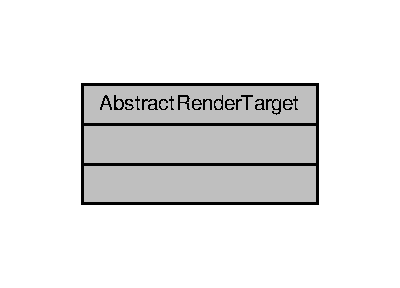
\includegraphics[width=192pt]{class_abstract_render_target__coll__graph}
\end{center}
\end{figure}


\subsection{Detailed Description}
Abstract base class for Open\-G\-L Objects. 

\begin{DoxyAuthor}{Author}
Declan Russell 
\end{DoxyAuthor}
\begin{DoxyDate}{Date}
28/04/2015 
\end{DoxyDate}
\begin{DoxyVersion}{Version}
1.\-0 
\end{DoxyVersion}


The documentation for this class was generated from the following file\-:\begin{DoxyCompactItemize}
\item 
/home/dexternation/\-A\-G\-S\-D\-T\-Fluid\-Sim/include/Abstract\-Open\-G\-L\-Object.\-h\end{DoxyCompactItemize}

\hypertarget{classbilateral_filter_frag}{\section{bilateral\-Filter\-Frag Class Reference}
\label{classbilateral_filter_frag}\index{bilateral\-Filter\-Frag@{bilateral\-Filter\-Frag}}
}


Fragment shader to apply bilateral filter blur on an input.  




Collaboration diagram for bilateral\-Filter\-Frag\-:\nopagebreak
\begin{figure}[H]
\begin{center}
\leavevmode
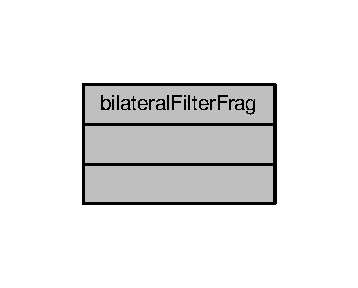
\includegraphics[width=172pt]{classbilateral_filter_frag__coll__graph}
\end{center}
\end{figure}


\subsection{Detailed Description}
Fragment shader to apply bilateral filter blur on an input. 

The documentation for this class was generated from the following file\-:\begin{DoxyCompactItemize}
\item 
/home/dexternation/\-A\-G\-S\-D\-T\-Fluid\-Sim/shaders/\hyperlink{bilateral_filter_frag_8glsl}{bilateral\-Filter\-Frag.\-glsl}\end{DoxyCompactItemize}

\hypertarget{classbilateral_filter_vert}{\section{bilateral\-Filter\-Vert Class Reference}
\label{classbilateral_filter_vert}\index{bilateral\-Filter\-Vert@{bilateral\-Filter\-Vert}}
}


Vertex shader for our bilateral filter shader. Just passes through positions and tex coords.  




Collaboration diagram for bilateral\-Filter\-Vert\-:\nopagebreak
\begin{figure}[H]
\begin{center}
\leavevmode
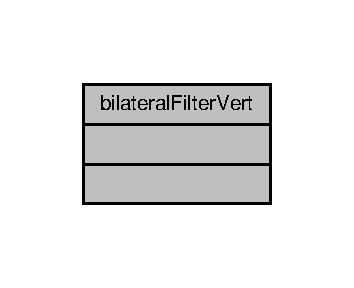
\includegraphics[width=170pt]{classbilateral_filter_vert__coll__graph}
\end{center}
\end{figure}


\subsection{Detailed Description}
Vertex shader for our bilateral filter shader. Just passes through positions and tex coords. 

The documentation for this class was generated from the following file\-:\begin{DoxyCompactItemize}
\item 
/home/dexternation/\-A\-G\-S\-D\-T\-Fluid\-Sim/shaders/\hyperlink{bilateral_filter_vert_8glsl}{bilateral\-Filter\-Vert.\-glsl}\end{DoxyCompactItemize}

\hypertarget{classcuboid_geom}{\section{cuboid\-Geom Class Reference}
\label{classcuboid_geom}\index{cuboid\-Geom@{cuboid\-Geom}}
}


Geometry shader for our cuboid shader. Turns one point into a cube drawn with G\-L\-\_\-\-L\-I\-N\-E\-S.  




Collaboration diagram for cuboid\-Geom\-:\nopagebreak
\begin{figure}[H]
\begin{center}
\leavevmode
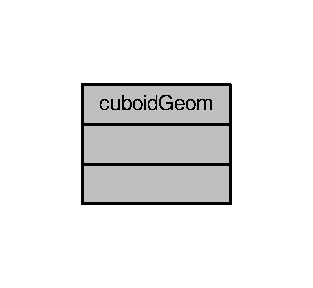
\includegraphics[width=150pt]{classcuboid_geom__coll__graph}
\end{center}
\end{figure}


\subsection{Detailed Description}
Geometry shader for our cuboid shader. Turns one point into a cube drawn with G\-L\-\_\-\-L\-I\-N\-E\-S. 

\begin{DoxyAuthor}{Author}
Declan Russell 
\end{DoxyAuthor}
\begin{DoxyDate}{Date}
2/05/15 
\end{DoxyDate}
\begin{DoxyVersion}{Version}
1.\-0  G\-L\-S\-L 
\end{DoxyVersion}


The documentation for this class was generated from the following file\-:\begin{DoxyCompactItemize}
\item 
/home/dexternation/\-A\-G\-S\-D\-T\-Fluid\-Sim/shaders/\hyperlink{cuboid_geom_8glsl}{cuboid\-Geom.\-glsl}\end{DoxyCompactItemize}

\hypertarget{classcuboid_vert}{\section{cuboid\-Vert Class Reference}
\label{classcuboid_vert}\index{cuboid\-Vert@{cuboid\-Vert}}
}


Vertex shader for our cuboid shader.  




Collaboration diagram for cuboid\-Vert\-:\nopagebreak
\begin{figure}[H]
\begin{center}
\leavevmode
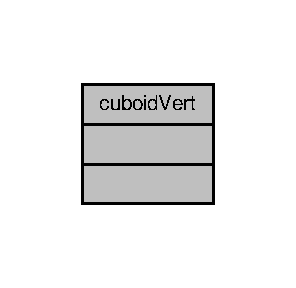
\includegraphics[width=142pt]{classcuboid_vert__coll__graph}
\end{center}
\end{figure}


\subsection{Detailed Description}
Vertex shader for our cuboid shader. 

\begin{DoxyAuthor}{Author}
Declan Russell 
\end{DoxyAuthor}
\begin{DoxyDate}{Date}
2/05/15 
\end{DoxyDate}
\begin{DoxyVersion}{Version}
1.\-0  G\-L\-S\-L 
\end{DoxyVersion}


The documentation for this class was generated from the following file\-:\begin{DoxyCompactItemize}
\item 
/home/dexternation/\-A\-G\-S\-D\-T\-Fluid\-Sim/shaders/\hyperlink{cuboid_vert_8glsl}{cuboid\-Vert.\-glsl}\end{DoxyCompactItemize}

\hypertarget{class_fluid_prop_dock_widget}{\section{Fluid\-Prop\-Dock\-Widget Class Reference}
\label{class_fluid_prop_dock_widget}\index{Fluid\-Prop\-Dock\-Widget@{Fluid\-Prop\-Dock\-Widget}}
}


Inheritance diagram for Fluid\-Prop\-Dock\-Widget\-:\nopagebreak
\begin{figure}[H]
\begin{center}
\leavevmode
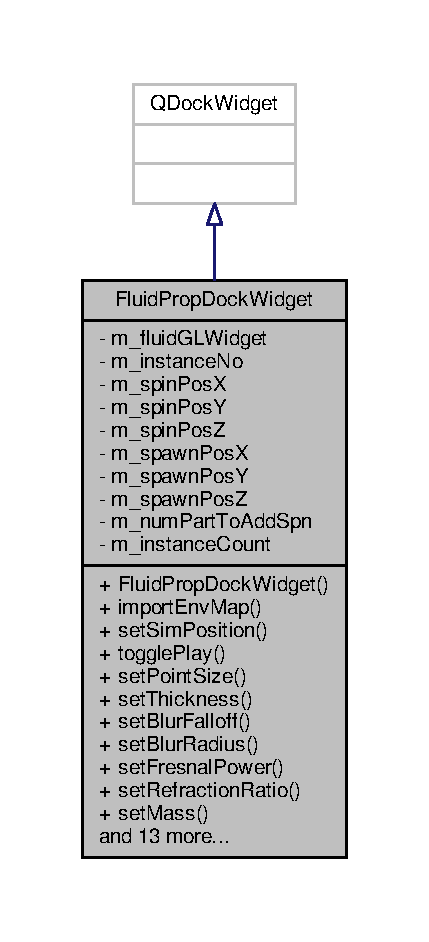
\includegraphics[width=206pt]{class_fluid_prop_dock_widget__inherit__graph}
\end{center}
\end{figure}


Collaboration diagram for Fluid\-Prop\-Dock\-Widget\-:\nopagebreak
\begin{figure}[H]
\begin{center}
\leavevmode
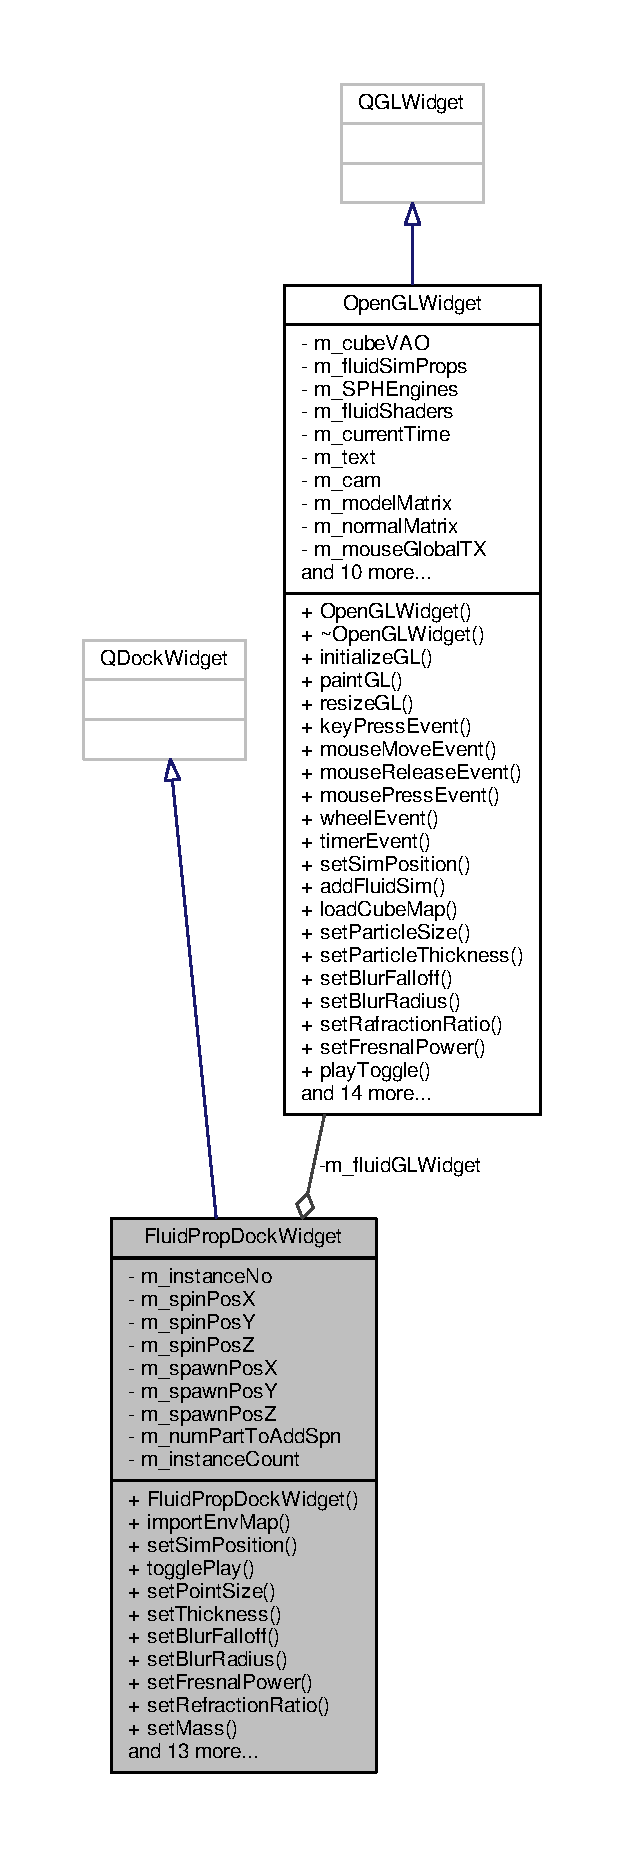
\includegraphics[height=550pt]{class_fluid_prop_dock_widget__coll__graph}
\end{center}
\end{figure}
\subsection*{Public Slots}
\begin{DoxyCompactItemize}
\item 
\hypertarget{class_fluid_prop_dock_widget_ab9c0a7c3635a4cbf4ab44229df363e48}{void \hyperlink{class_fluid_prop_dock_widget_ab9c0a7c3635a4cbf4ab44229df363e48}{import\-Env\-Map} ()}\label{class_fluid_prop_dock_widget_ab9c0a7c3635a4cbf4ab44229df363e48}

\begin{DoxyCompactList}\small\item\em slot to change our environment map \end{DoxyCompactList}\item 
\hypertarget{class_fluid_prop_dock_widget_aa4d9a3ef7ced0c9864550554fdc626b1}{void \hyperlink{class_fluid_prop_dock_widget_aa4d9a3ef7ced0c9864550554fdc626b1}{set\-Sim\-Position} ()}\label{class_fluid_prop_dock_widget_aa4d9a3ef7ced0c9864550554fdc626b1}

\begin{DoxyCompactList}\small\item\em slot to set the simulation postion \end{DoxyCompactList}\item 
\hypertarget{class_fluid_prop_dock_widget_a16076f5d56b8d79f74726915d0f51b0b}{void \hyperlink{class_fluid_prop_dock_widget_a16076f5d56b8d79f74726915d0f51b0b}{toggle\-Play} ()}\label{class_fluid_prop_dock_widget_a16076f5d56b8d79f74726915d0f51b0b}

\begin{DoxyCompactList}\small\item\em slot to toggle play of our simulation \end{DoxyCompactList}\item 
void \hyperlink{class_fluid_prop_dock_widget_afeb4fe68de9245e8fc3696870ed239b1}{set\-Point\-Size} (double \-\_\-size)
\begin{DoxyCompactList}\small\item\em slot to set the point size of our simulation \end{DoxyCompactList}\item 
void \hyperlink{class_fluid_prop_dock_widget_a350d3512b0f415f51ea121e6f1136028}{set\-Thickness} (double \-\_\-thickness)
\begin{DoxyCompactList}\small\item\em slot to set the thickness or the particles in our simulation \end{DoxyCompactList}\item 
void \hyperlink{class_fluid_prop_dock_widget_ae7b93e96ca395cbd0301ec297480ee04}{set\-Blur\-Falloff} (double \-\_\-falloff)
\begin{DoxyCompactList}\small\item\em slot to set our bilateral filter blur fall off \end{DoxyCompactList}\item 
void \hyperlink{class_fluid_prop_dock_widget_a2ae578e791a6768c99dc8e2e297ea4bb}{set\-Blur\-Radius} (double \-\_\-radius)
\begin{DoxyCompactList}\small\item\em slot to set our bilateral filter blur radius \end{DoxyCompactList}\item 
void \hyperlink{class_fluid_prop_dock_widget_a7993dd47f7e625c8b1a3f12def0d1d72}{set\-Fresnal\-Power} (double \-\_\-power)
\begin{DoxyCompactList}\small\item\em slot to set the fresnal power of our fluid \end{DoxyCompactList}\item 
void \hyperlink{class_fluid_prop_dock_widget_a2f07e4371b46ccbd7c649264e94646de}{set\-Refraction\-Ratio} (double \-\_\-eta)
\begin{DoxyCompactList}\small\item\em slot to set the refraction ratio of our fluid \end{DoxyCompactList}\item 
void \hyperlink{class_fluid_prop_dock_widget_ae4ee0f4372a699416af91c0b111e95fe}{set\-Mass} (double \-\_\-mass)
\begin{DoxyCompactList}\small\item\em slot to set the mass of our fluid \end{DoxyCompactList}\item 
void \hyperlink{class_fluid_prop_dock_widget_af8a936150aa411f15498bce8c8bd409f}{set\-Density} (double \-\_\-density)
\begin{DoxyCompactList}\small\item\em slot to set the rest density of our fluid \end{DoxyCompactList}\item 
void \hyperlink{class_fluid_prop_dock_widget_a473ce1156c2ab118e6af5d99ec700764}{set\-Viscosity} (double \-\_\-visc)
\begin{DoxyCompactList}\small\item\em slot to set the viscosity coeficient of our fluid \end{DoxyCompactList}\item 
void \hyperlink{class_fluid_prop_dock_widget_aa9cb10cd748f9bce2f751e535bc5a286}{set\-Gas\-Const} (double \-\_\-gconst)
\begin{DoxyCompactList}\small\item\em slot to set the gas constant of our fluid \end{DoxyCompactList}\item 
void \hyperlink{class_fluid_prop_dock_widget_a04366783099838b9a2b364ecd3d53da3}{set\-Smoothing\-Length} (double \-\_\-len)
\begin{DoxyCompactList}\small\item\em slot to set the smoothing length of our fluid simulation \end{DoxyCompactList}\item 
void \hyperlink{class_fluid_prop_dock_widget_aa17ebb5265733ed6d0bb6d7f5305c687}{set\-Fluid\-Color} (Q\-Color \-\_\-col)
\begin{DoxyCompactList}\small\item\em slot to set the color of our fluid \end{DoxyCompactList}\item 
void \hyperlink{class_fluid_prop_dock_widget_a6264d4d89eeeb8adf5bec124598fbcf1}{set\-Playback\-Speed} (int \-\_\-speed)
\begin{DoxyCompactList}\small\item\em slot to set the play back speed of our simulation \end{DoxyCompactList}\item 
\hypertarget{class_fluid_prop_dock_widget_aba723bc2dc92241efbde8434ab3f711b}{void \hyperlink{class_fluid_prop_dock_widget_aba723bc2dc92241efbde8434ab3f711b}{reset\-Sim} ()}\label{class_fluid_prop_dock_widget_aba723bc2dc92241efbde8434ab3f711b}

\begin{DoxyCompactList}\small\item\em slot to reset our simulation \end{DoxyCompactList}\item 
void \hyperlink{class_fluid_prop_dock_widget_ae59c72dfb12faf77940e805e94b78cbf}{set\-Spawn\-Box\-Size} (double \-\_\-size)
\begin{DoxyCompactList}\small\item\em slot to set the spawn box size \end{DoxyCompactList}\item 
\hypertarget{class_fluid_prop_dock_widget_a1e3b987049f5f5ff5958a7cd3dcdbdff}{void \hyperlink{class_fluid_prop_dock_widget_a1e3b987049f5f5ff5958a7cd3dcdbdff}{add\-Part\-To\-Sim} ()}\label{class_fluid_prop_dock_widget_a1e3b987049f5f5ff5958a7cd3dcdbdff}

\begin{DoxyCompactList}\small\item\em slot to add particles to our simulation \end{DoxyCompactList}\item 
\hypertarget{class_fluid_prop_dock_widget_aac86685277d0b7f6c631e5f53efdc247}{void \hyperlink{class_fluid_prop_dock_widget_aac86685277d0b7f6c631e5f53efdc247}{set\-Spawn\-Box\-Pos} ()}\label{class_fluid_prop_dock_widget_aac86685277d0b7f6c631e5f53efdc247}

\begin{DoxyCompactList}\small\item\em slot to set the spawn box position \end{DoxyCompactList}\item 
void \hyperlink{class_fluid_prop_dock_widget_a03628de74620c25af71461a255163a84}{set\-Time\-Step} (double \-\_\-step)
\begin{DoxyCompactList}\small\item\em slot to set the time step our simulation \end{DoxyCompactList}\item 
void \hyperlink{class_fluid_prop_dock_widget_a7c06460036dcca6716dea7b7fc70ad66}{set\-Vel\-Correction} (double \-\_\-val)
\begin{DoxyCompactList}\small\item\em slot to set the velocity correction of our simulatin \end{DoxyCompactList}\item 
void \hyperlink{class_fluid_prop_dock_widget_a6e6423b9cdf21dd02577b72339d5babd}{set\-Display\-Hud} (bool \-\_\-display)
\begin{DoxyCompactList}\small\item\em slot to toggle the hud of our simulation \end{DoxyCompactList}\end{DoxyCompactItemize}
\subsection*{Public Member Functions}
\begin{DoxyCompactItemize}
\item 
\hyperlink{class_fluid_prop_dock_widget_a48fd1ee2a02d9ca27f905d556ce23075}{Fluid\-Prop\-Dock\-Widget} (\hyperlink{class_open_g_l_widget}{Open\-G\-L\-Widget} $\ast$\-\_\-fluid\-Widget, Q\-Widget $\ast$parent=0)
\begin{DoxyCompactList}\small\item\em default constructor. \end{DoxyCompactList}\end{DoxyCompactItemize}
\subsection*{Private Attributes}
\begin{DoxyCompactItemize}
\item 
\hypertarget{class_fluid_prop_dock_widget_a4c4c2a709cbe2075aec6515d0dc3827f}{\hyperlink{class_open_g_l_widget}{Open\-G\-L\-Widget} $\ast$ \hyperlink{class_fluid_prop_dock_widget_a4c4c2a709cbe2075aec6515d0dc3827f}{m\-\_\-fluid\-G\-L\-Widget}}\label{class_fluid_prop_dock_widget_a4c4c2a709cbe2075aec6515d0dc3827f}

\begin{DoxyCompactList}\small\item\em a pointer to our fluid sim open\-Gl\-Widget \end{DoxyCompactList}\item 
\hypertarget{class_fluid_prop_dock_widget_aeb7969c3b9eda8f9c5bd321c0595365f}{int \hyperlink{class_fluid_prop_dock_widget_aeb7969c3b9eda8f9c5bd321c0595365f}{m\-\_\-instance\-No}}\label{class_fluid_prop_dock_widget_aeb7969c3b9eda8f9c5bd321c0595365f}

\begin{DoxyCompactList}\small\item\em instance number \end{DoxyCompactList}\item 
\hypertarget{class_fluid_prop_dock_widget_a771c88921c30df2716850909d7874750}{Q\-Double\-Spin\-Box $\ast$ \hyperlink{class_fluid_prop_dock_widget_a771c88921c30df2716850909d7874750}{m\-\_\-spin\-Pos\-X}}\label{class_fluid_prop_dock_widget_a771c88921c30df2716850909d7874750}

\begin{DoxyCompactList}\small\item\em sim postion x \end{DoxyCompactList}\item 
\hypertarget{class_fluid_prop_dock_widget_a9023519e1ec5b0e60c2f3f2a705298ae}{Q\-Double\-Spin\-Box $\ast$ \hyperlink{class_fluid_prop_dock_widget_a9023519e1ec5b0e60c2f3f2a705298ae}{m\-\_\-spin\-Pos\-Y}}\label{class_fluid_prop_dock_widget_a9023519e1ec5b0e60c2f3f2a705298ae}

\begin{DoxyCompactList}\small\item\em sim postion y \end{DoxyCompactList}\item 
\hypertarget{class_fluid_prop_dock_widget_a4e544ec628583e2b587e22f6c08369ab}{Q\-Double\-Spin\-Box $\ast$ \hyperlink{class_fluid_prop_dock_widget_a4e544ec628583e2b587e22f6c08369ab}{m\-\_\-spin\-Pos\-Z}}\label{class_fluid_prop_dock_widget_a4e544ec628583e2b587e22f6c08369ab}

\begin{DoxyCompactList}\small\item\em sim postion z \end{DoxyCompactList}\item 
\hypertarget{class_fluid_prop_dock_widget_af29dabe6b5caab6510415ff01ac6bc80}{Q\-Double\-Spin\-Box $\ast$ \hyperlink{class_fluid_prop_dock_widget_af29dabe6b5caab6510415ff01ac6bc80}{m\-\_\-spawn\-Pos\-X}}\label{class_fluid_prop_dock_widget_af29dabe6b5caab6510415ff01ac6bc80}

\begin{DoxyCompactList}\small\item\em spawn box position x \end{DoxyCompactList}\item 
\hypertarget{class_fluid_prop_dock_widget_a8f2f0459bf7cab6f0f4184b538dbb0c0}{Q\-Double\-Spin\-Box $\ast$ \hyperlink{class_fluid_prop_dock_widget_a8f2f0459bf7cab6f0f4184b538dbb0c0}{m\-\_\-spawn\-Pos\-Y}}\label{class_fluid_prop_dock_widget_a8f2f0459bf7cab6f0f4184b538dbb0c0}

\begin{DoxyCompactList}\small\item\em spawn box position y \end{DoxyCompactList}\item 
\hypertarget{class_fluid_prop_dock_widget_a520d14921acb438e884ef66d4d702921}{Q\-Double\-Spin\-Box $\ast$ \hyperlink{class_fluid_prop_dock_widget_a520d14921acb438e884ef66d4d702921}{m\-\_\-spawn\-Pos\-Z}}\label{class_fluid_prop_dock_widget_a520d14921acb438e884ef66d4d702921}

\begin{DoxyCompactList}\small\item\em spawn box position z \end{DoxyCompactList}\item 
\hypertarget{class_fluid_prop_dock_widget_af5ae6a4d95070ebdd3a0dd434cbdeb48}{Q\-Spin\-Box $\ast$ \hyperlink{class_fluid_prop_dock_widget_af5ae6a4d95070ebdd3a0dd434cbdeb48}{m\-\_\-num\-Part\-To\-Add\-Spn}}\label{class_fluid_prop_dock_widget_af5ae6a4d95070ebdd3a0dd434cbdeb48}

\begin{DoxyCompactList}\small\item\em spinbox for the number of particles to add to the simulation \end{DoxyCompactList}\end{DoxyCompactItemize}
\subsection*{Static Private Attributes}
\begin{DoxyCompactItemize}
\item 
\hypertarget{class_fluid_prop_dock_widget_a1a99d39cc50119d25df70e17c0d525ed}{static int \hyperlink{class_fluid_prop_dock_widget_a1a99d39cc50119d25df70e17c0d525ed}{m\-\_\-instance\-Count}}\label{class_fluid_prop_dock_widget_a1a99d39cc50119d25df70e17c0d525ed}

\begin{DoxyCompactList}\small\item\em a static member to keep track of how many instances we have \end{DoxyCompactList}\end{DoxyCompactItemize}


\subsection{Constructor \& Destructor Documentation}
\hypertarget{class_fluid_prop_dock_widget_a48fd1ee2a02d9ca27f905d556ce23075}{\index{Fluid\-Prop\-Dock\-Widget@{Fluid\-Prop\-Dock\-Widget}!Fluid\-Prop\-Dock\-Widget@{Fluid\-Prop\-Dock\-Widget}}
\index{Fluid\-Prop\-Dock\-Widget@{Fluid\-Prop\-Dock\-Widget}!FluidPropDockWidget@{Fluid\-Prop\-Dock\-Widget}}
\subsubsection[{Fluid\-Prop\-Dock\-Widget}]{\setlength{\rightskip}{0pt plus 5cm}Fluid\-Prop\-Dock\-Widget\-::\-Fluid\-Prop\-Dock\-Widget (
\begin{DoxyParamCaption}
\item[{{\bf Open\-G\-L\-Widget} $\ast$}]{\-\_\-fluid\-Widget, }
\item[{Q\-Widget $\ast$}]{parent = {\ttfamily 0}}
\end{DoxyParamCaption}
)\hspace{0.3cm}{\ttfamily [explicit]}}}\label{class_fluid_prop_dock_widget_a48fd1ee2a02d9ca27f905d556ce23075}


default constructor. 


\begin{DoxyParams}{Parameters}
{\em \-\_\-fluid\-Widget} & -\/ \hyperlink{class_open_g_l_widget}{Open\-G\-L\-Widget} used for our fluid sim \\
\hline
\end{DoxyParams}


Here is the call graph for this function\-:\nopagebreak
\begin{figure}[H]
\begin{center}
\leavevmode
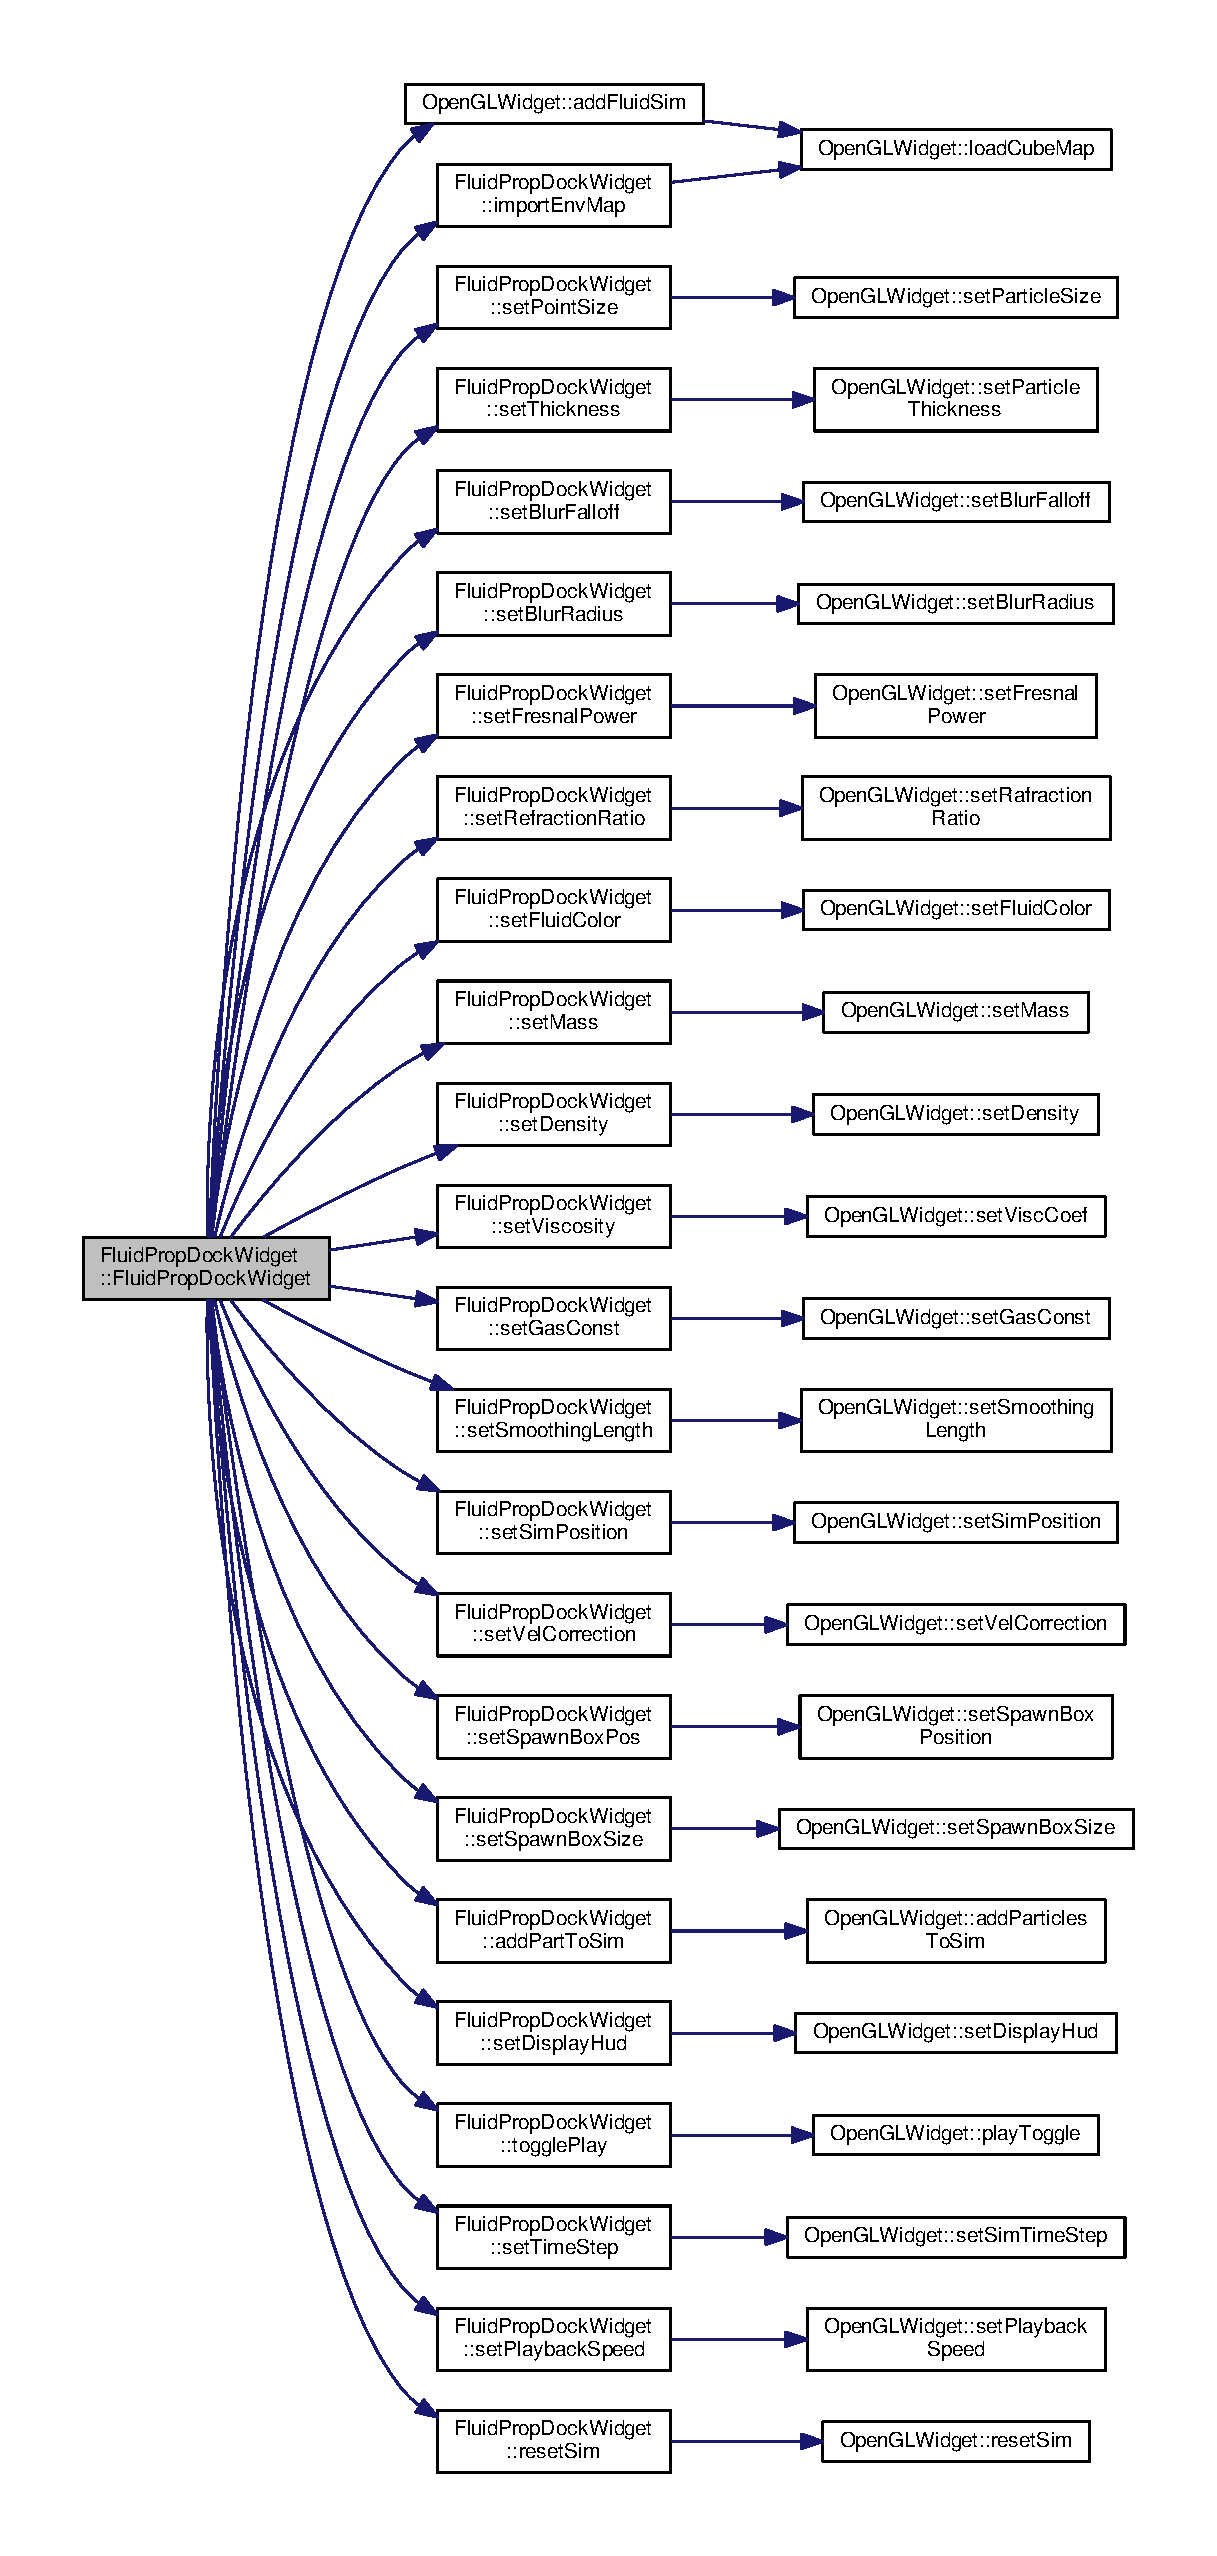
\includegraphics[height=550pt]{class_fluid_prop_dock_widget_a48fd1ee2a02d9ca27f905d556ce23075_cgraph}
\end{center}
\end{figure}




\subsection{Member Function Documentation}
\hypertarget{class_fluid_prop_dock_widget_ae7b93e96ca395cbd0301ec297480ee04}{\index{Fluid\-Prop\-Dock\-Widget@{Fluid\-Prop\-Dock\-Widget}!set\-Blur\-Falloff@{set\-Blur\-Falloff}}
\index{set\-Blur\-Falloff@{set\-Blur\-Falloff}!FluidPropDockWidget@{Fluid\-Prop\-Dock\-Widget}}
\subsubsection[{set\-Blur\-Falloff}]{\setlength{\rightskip}{0pt plus 5cm}void Fluid\-Prop\-Dock\-Widget\-::set\-Blur\-Falloff (
\begin{DoxyParamCaption}
\item[{double}]{\-\_\-falloff}
\end{DoxyParamCaption}
)\hspace{0.3cm}{\ttfamily [inline]}, {\ttfamily [slot]}}}\label{class_fluid_prop_dock_widget_ae7b93e96ca395cbd0301ec297480ee04}


slot to set our bilateral filter blur fall off 


\begin{DoxyParams}{Parameters}
{\em \-\_\-falloff} & -\/ desired blur fall off \\
\hline
\end{DoxyParams}


Here is the call graph for this function\-:\nopagebreak
\begin{figure}[H]
\begin{center}
\leavevmode
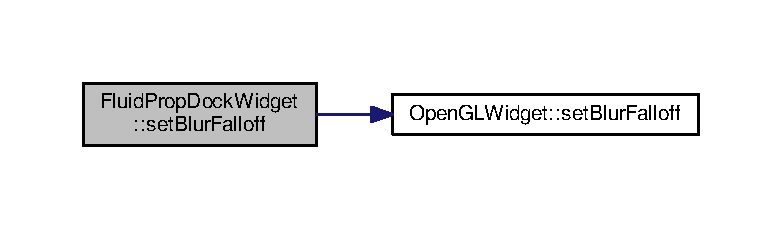
\includegraphics[width=350pt]{class_fluid_prop_dock_widget_ae7b93e96ca395cbd0301ec297480ee04_cgraph}
\end{center}
\end{figure}




Here is the caller graph for this function\-:\nopagebreak
\begin{figure}[H]
\begin{center}
\leavevmode
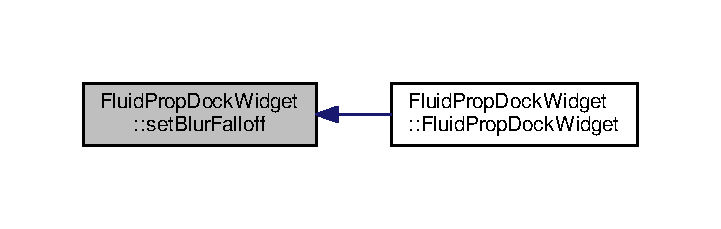
\includegraphics[width=346pt]{class_fluid_prop_dock_widget_ae7b93e96ca395cbd0301ec297480ee04_icgraph}
\end{center}
\end{figure}


\hypertarget{class_fluid_prop_dock_widget_a2ae578e791a6768c99dc8e2e297ea4bb}{\index{Fluid\-Prop\-Dock\-Widget@{Fluid\-Prop\-Dock\-Widget}!set\-Blur\-Radius@{set\-Blur\-Radius}}
\index{set\-Blur\-Radius@{set\-Blur\-Radius}!FluidPropDockWidget@{Fluid\-Prop\-Dock\-Widget}}
\subsubsection[{set\-Blur\-Radius}]{\setlength{\rightskip}{0pt plus 5cm}void Fluid\-Prop\-Dock\-Widget\-::set\-Blur\-Radius (
\begin{DoxyParamCaption}
\item[{double}]{\-\_\-radius}
\end{DoxyParamCaption}
)\hspace{0.3cm}{\ttfamily [inline]}, {\ttfamily [slot]}}}\label{class_fluid_prop_dock_widget_a2ae578e791a6768c99dc8e2e297ea4bb}


slot to set our bilateral filter blur radius 


\begin{DoxyParams}{Parameters}
{\em \-\_\-radius} & -\/ desired blur radius \\
\hline
\end{DoxyParams}


Here is the call graph for this function\-:\nopagebreak
\begin{figure}[H]
\begin{center}
\leavevmode
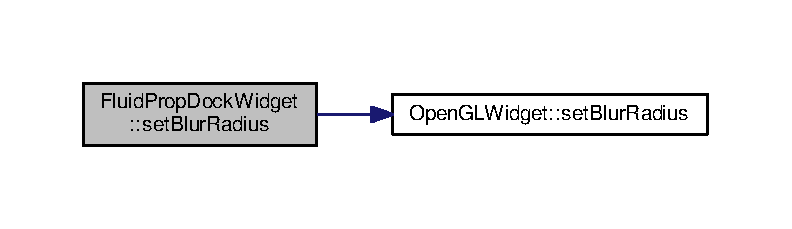
\includegraphics[width=350pt]{class_fluid_prop_dock_widget_a2ae578e791a6768c99dc8e2e297ea4bb_cgraph}
\end{center}
\end{figure}




Here is the caller graph for this function\-:\nopagebreak
\begin{figure}[H]
\begin{center}
\leavevmode
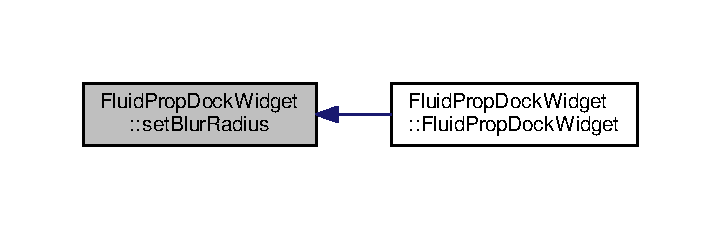
\includegraphics[width=346pt]{class_fluid_prop_dock_widget_a2ae578e791a6768c99dc8e2e297ea4bb_icgraph}
\end{center}
\end{figure}


\hypertarget{class_fluid_prop_dock_widget_af8a936150aa411f15498bce8c8bd409f}{\index{Fluid\-Prop\-Dock\-Widget@{Fluid\-Prop\-Dock\-Widget}!set\-Density@{set\-Density}}
\index{set\-Density@{set\-Density}!FluidPropDockWidget@{Fluid\-Prop\-Dock\-Widget}}
\subsubsection[{set\-Density}]{\setlength{\rightskip}{0pt plus 5cm}void Fluid\-Prop\-Dock\-Widget\-::set\-Density (
\begin{DoxyParamCaption}
\item[{double}]{\-\_\-density}
\end{DoxyParamCaption}
)\hspace{0.3cm}{\ttfamily [inline]}, {\ttfamily [slot]}}}\label{class_fluid_prop_dock_widget_af8a936150aa411f15498bce8c8bd409f}


slot to set the rest density of our fluid 


\begin{DoxyParams}{Parameters}
{\em \-\_\-density} & -\/ desired rest density of of fluid \\
\hline
\end{DoxyParams}


Here is the call graph for this function\-:\nopagebreak
\begin{figure}[H]
\begin{center}
\leavevmode
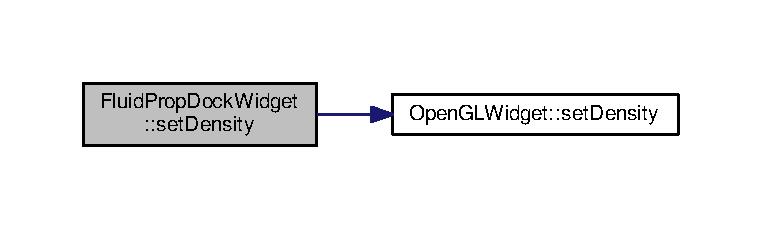
\includegraphics[width=350pt]{class_fluid_prop_dock_widget_af8a936150aa411f15498bce8c8bd409f_cgraph}
\end{center}
\end{figure}




Here is the caller graph for this function\-:\nopagebreak
\begin{figure}[H]
\begin{center}
\leavevmode
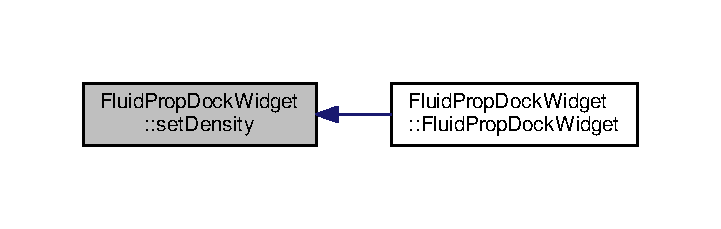
\includegraphics[width=346pt]{class_fluid_prop_dock_widget_af8a936150aa411f15498bce8c8bd409f_icgraph}
\end{center}
\end{figure}


\hypertarget{class_fluid_prop_dock_widget_a6e6423b9cdf21dd02577b72339d5babd}{\index{Fluid\-Prop\-Dock\-Widget@{Fluid\-Prop\-Dock\-Widget}!set\-Display\-Hud@{set\-Display\-Hud}}
\index{set\-Display\-Hud@{set\-Display\-Hud}!FluidPropDockWidget@{Fluid\-Prop\-Dock\-Widget}}
\subsubsection[{set\-Display\-Hud}]{\setlength{\rightskip}{0pt plus 5cm}void Fluid\-Prop\-Dock\-Widget\-::set\-Display\-Hud (
\begin{DoxyParamCaption}
\item[{bool}]{\-\_\-display}
\end{DoxyParamCaption}
)\hspace{0.3cm}{\ttfamily [inline]}, {\ttfamily [slot]}}}\label{class_fluid_prop_dock_widget_a6e6423b9cdf21dd02577b72339d5babd}


slot to toggle the hud of our simulation 


\begin{DoxyParams}{Parameters}
{\em \-\_\-display} & -\/ bool to indicate if we want to display our hud \\
\hline
\end{DoxyParams}


Here is the call graph for this function\-:\nopagebreak
\begin{figure}[H]
\begin{center}
\leavevmode
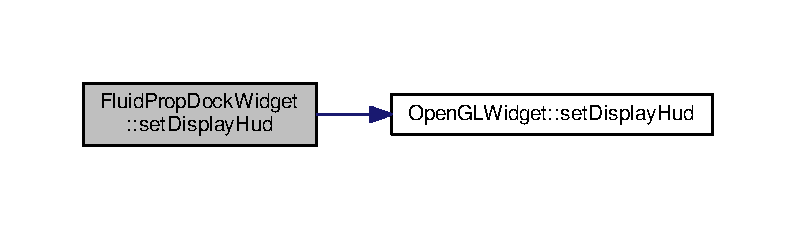
\includegraphics[width=350pt]{class_fluid_prop_dock_widget_a6e6423b9cdf21dd02577b72339d5babd_cgraph}
\end{center}
\end{figure}




Here is the caller graph for this function\-:\nopagebreak
\begin{figure}[H]
\begin{center}
\leavevmode
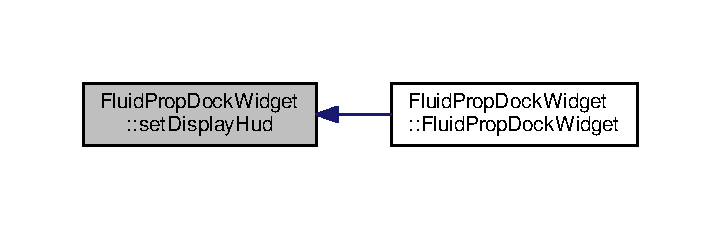
\includegraphics[width=346pt]{class_fluid_prop_dock_widget_a6e6423b9cdf21dd02577b72339d5babd_icgraph}
\end{center}
\end{figure}


\hypertarget{class_fluid_prop_dock_widget_aa17ebb5265733ed6d0bb6d7f5305c687}{\index{Fluid\-Prop\-Dock\-Widget@{Fluid\-Prop\-Dock\-Widget}!set\-Fluid\-Color@{set\-Fluid\-Color}}
\index{set\-Fluid\-Color@{set\-Fluid\-Color}!FluidPropDockWidget@{Fluid\-Prop\-Dock\-Widget}}
\subsubsection[{set\-Fluid\-Color}]{\setlength{\rightskip}{0pt plus 5cm}void Fluid\-Prop\-Dock\-Widget\-::set\-Fluid\-Color (
\begin{DoxyParamCaption}
\item[{Q\-Color}]{\-\_\-col}
\end{DoxyParamCaption}
)\hspace{0.3cm}{\ttfamily [inline]}, {\ttfamily [slot]}}}\label{class_fluid_prop_dock_widget_aa17ebb5265733ed6d0bb6d7f5305c687}


slot to set the color of our fluid 


\begin{DoxyParams}{Parameters}
{\em \-\_\-col} & -\/ desired color of fluid \\
\hline
\end{DoxyParams}


Here is the call graph for this function\-:\nopagebreak
\begin{figure}[H]
\begin{center}
\leavevmode
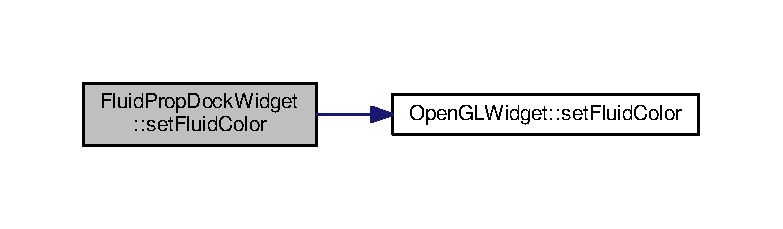
\includegraphics[width=350pt]{class_fluid_prop_dock_widget_aa17ebb5265733ed6d0bb6d7f5305c687_cgraph}
\end{center}
\end{figure}




Here is the caller graph for this function\-:\nopagebreak
\begin{figure}[H]
\begin{center}
\leavevmode
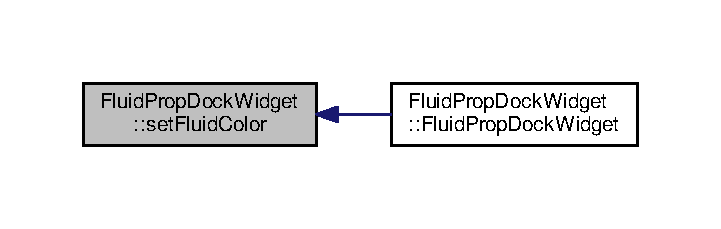
\includegraphics[width=346pt]{class_fluid_prop_dock_widget_aa17ebb5265733ed6d0bb6d7f5305c687_icgraph}
\end{center}
\end{figure}


\hypertarget{class_fluid_prop_dock_widget_a7993dd47f7e625c8b1a3f12def0d1d72}{\index{Fluid\-Prop\-Dock\-Widget@{Fluid\-Prop\-Dock\-Widget}!set\-Fresnal\-Power@{set\-Fresnal\-Power}}
\index{set\-Fresnal\-Power@{set\-Fresnal\-Power}!FluidPropDockWidget@{Fluid\-Prop\-Dock\-Widget}}
\subsubsection[{set\-Fresnal\-Power}]{\setlength{\rightskip}{0pt plus 5cm}void Fluid\-Prop\-Dock\-Widget\-::set\-Fresnal\-Power (
\begin{DoxyParamCaption}
\item[{double}]{\-\_\-power}
\end{DoxyParamCaption}
)\hspace{0.3cm}{\ttfamily [inline]}, {\ttfamily [slot]}}}\label{class_fluid_prop_dock_widget_a7993dd47f7e625c8b1a3f12def0d1d72}


slot to set the fresnal power of our fluid 


\begin{DoxyParams}{Parameters}
{\em \-\_\-power} & -\/ desired fresnal power \\
\hline
\end{DoxyParams}


Here is the call graph for this function\-:\nopagebreak
\begin{figure}[H]
\begin{center}
\leavevmode
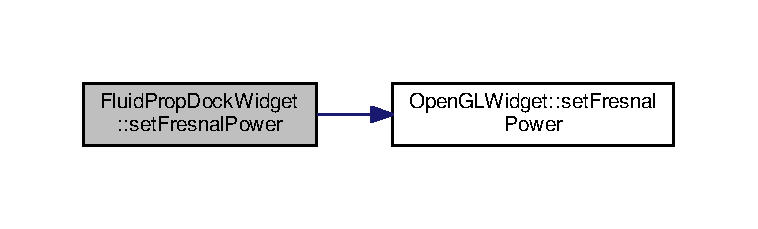
\includegraphics[width=350pt]{class_fluid_prop_dock_widget_a7993dd47f7e625c8b1a3f12def0d1d72_cgraph}
\end{center}
\end{figure}




Here is the caller graph for this function\-:\nopagebreak
\begin{figure}[H]
\begin{center}
\leavevmode
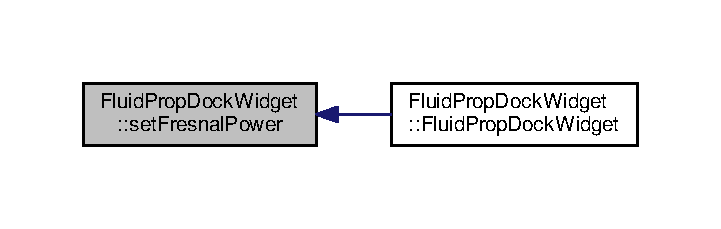
\includegraphics[width=346pt]{class_fluid_prop_dock_widget_a7993dd47f7e625c8b1a3f12def0d1d72_icgraph}
\end{center}
\end{figure}


\hypertarget{class_fluid_prop_dock_widget_aa9cb10cd748f9bce2f751e535bc5a286}{\index{Fluid\-Prop\-Dock\-Widget@{Fluid\-Prop\-Dock\-Widget}!set\-Gas\-Const@{set\-Gas\-Const}}
\index{set\-Gas\-Const@{set\-Gas\-Const}!FluidPropDockWidget@{Fluid\-Prop\-Dock\-Widget}}
\subsubsection[{set\-Gas\-Const}]{\setlength{\rightskip}{0pt plus 5cm}void Fluid\-Prop\-Dock\-Widget\-::set\-Gas\-Const (
\begin{DoxyParamCaption}
\item[{double}]{\-\_\-gconst}
\end{DoxyParamCaption}
)\hspace{0.3cm}{\ttfamily [inline]}, {\ttfamily [slot]}}}\label{class_fluid_prop_dock_widget_aa9cb10cd748f9bce2f751e535bc5a286}


slot to set the gas constant of our fluid 


\begin{DoxyParams}{Parameters}
{\em \-\_\-gconst} & -\/ desired gas constant of fluid \\
\hline
\end{DoxyParams}


Here is the call graph for this function\-:\nopagebreak
\begin{figure}[H]
\begin{center}
\leavevmode
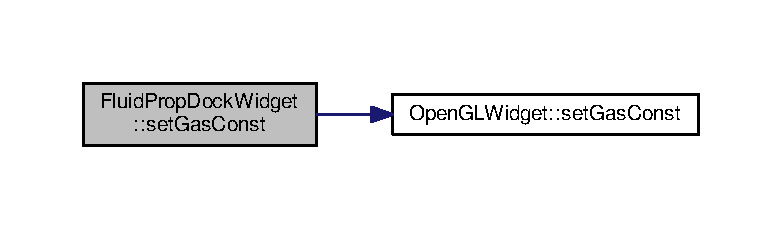
\includegraphics[width=350pt]{class_fluid_prop_dock_widget_aa9cb10cd748f9bce2f751e535bc5a286_cgraph}
\end{center}
\end{figure}




Here is the caller graph for this function\-:\nopagebreak
\begin{figure}[H]
\begin{center}
\leavevmode
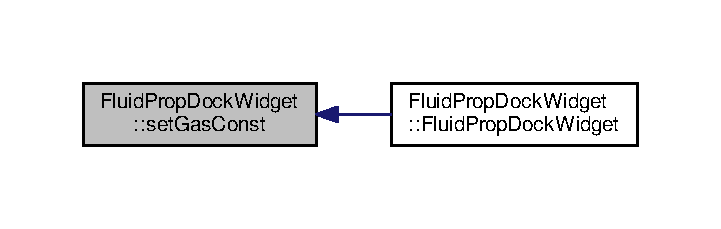
\includegraphics[width=346pt]{class_fluid_prop_dock_widget_aa9cb10cd748f9bce2f751e535bc5a286_icgraph}
\end{center}
\end{figure}


\hypertarget{class_fluid_prop_dock_widget_ae4ee0f4372a699416af91c0b111e95fe}{\index{Fluid\-Prop\-Dock\-Widget@{Fluid\-Prop\-Dock\-Widget}!set\-Mass@{set\-Mass}}
\index{set\-Mass@{set\-Mass}!FluidPropDockWidget@{Fluid\-Prop\-Dock\-Widget}}
\subsubsection[{set\-Mass}]{\setlength{\rightskip}{0pt plus 5cm}void Fluid\-Prop\-Dock\-Widget\-::set\-Mass (
\begin{DoxyParamCaption}
\item[{double}]{\-\_\-mass}
\end{DoxyParamCaption}
)\hspace{0.3cm}{\ttfamily [inline]}, {\ttfamily [slot]}}}\label{class_fluid_prop_dock_widget_ae4ee0f4372a699416af91c0b111e95fe}


slot to set the mass of our fluid 


\begin{DoxyParams}{Parameters}
{\em \-\_\-mass} & -\/ desired mass of fluid \\
\hline
\end{DoxyParams}


Here is the call graph for this function\-:\nopagebreak
\begin{figure}[H]
\begin{center}
\leavevmode
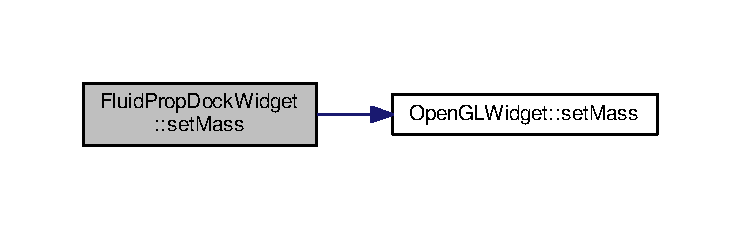
\includegraphics[width=350pt]{class_fluid_prop_dock_widget_ae4ee0f4372a699416af91c0b111e95fe_cgraph}
\end{center}
\end{figure}




Here is the caller graph for this function\-:\nopagebreak
\begin{figure}[H]
\begin{center}
\leavevmode
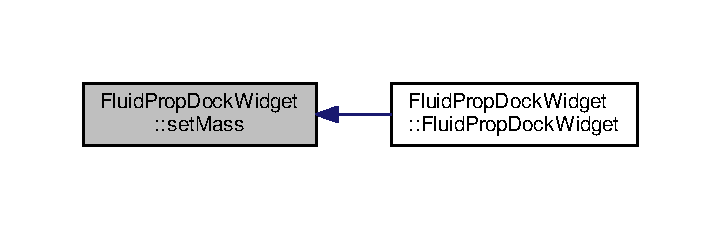
\includegraphics[width=346pt]{class_fluid_prop_dock_widget_ae4ee0f4372a699416af91c0b111e95fe_icgraph}
\end{center}
\end{figure}


\hypertarget{class_fluid_prop_dock_widget_a6264d4d89eeeb8adf5bec124598fbcf1}{\index{Fluid\-Prop\-Dock\-Widget@{Fluid\-Prop\-Dock\-Widget}!set\-Playback\-Speed@{set\-Playback\-Speed}}
\index{set\-Playback\-Speed@{set\-Playback\-Speed}!FluidPropDockWidget@{Fluid\-Prop\-Dock\-Widget}}
\subsubsection[{set\-Playback\-Speed}]{\setlength{\rightskip}{0pt plus 5cm}void Fluid\-Prop\-Dock\-Widget\-::set\-Playback\-Speed (
\begin{DoxyParamCaption}
\item[{int}]{\-\_\-speed}
\end{DoxyParamCaption}
)\hspace{0.3cm}{\ttfamily [inline]}, {\ttfamily [slot]}}}\label{class_fluid_prop_dock_widget_a6264d4d89eeeb8adf5bec124598fbcf1}


slot to set the play back speed of our simulation 


\begin{DoxyParams}{Parameters}
{\em \-\_\-speed} & -\/ desired speed of simulation as a absolute percentage \\
\hline
\end{DoxyParams}


Here is the call graph for this function\-:\nopagebreak
\begin{figure}[H]
\begin{center}
\leavevmode
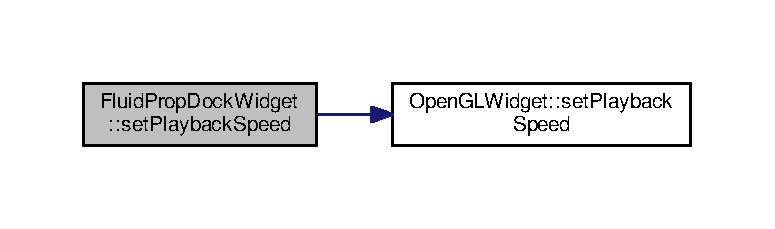
\includegraphics[width=350pt]{class_fluid_prop_dock_widget_a6264d4d89eeeb8adf5bec124598fbcf1_cgraph}
\end{center}
\end{figure}




Here is the caller graph for this function\-:\nopagebreak
\begin{figure}[H]
\begin{center}
\leavevmode
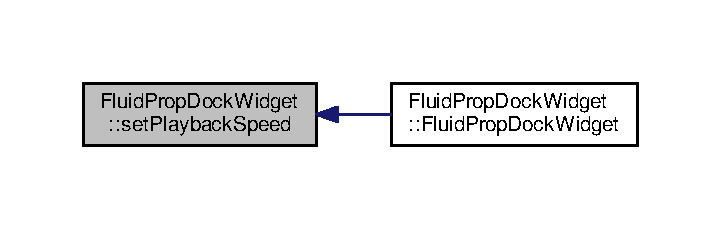
\includegraphics[width=346pt]{class_fluid_prop_dock_widget_a6264d4d89eeeb8adf5bec124598fbcf1_icgraph}
\end{center}
\end{figure}


\hypertarget{class_fluid_prop_dock_widget_afeb4fe68de9245e8fc3696870ed239b1}{\index{Fluid\-Prop\-Dock\-Widget@{Fluid\-Prop\-Dock\-Widget}!set\-Point\-Size@{set\-Point\-Size}}
\index{set\-Point\-Size@{set\-Point\-Size}!FluidPropDockWidget@{Fluid\-Prop\-Dock\-Widget}}
\subsubsection[{set\-Point\-Size}]{\setlength{\rightskip}{0pt plus 5cm}void Fluid\-Prop\-Dock\-Widget\-::set\-Point\-Size (
\begin{DoxyParamCaption}
\item[{double}]{\-\_\-size}
\end{DoxyParamCaption}
)\hspace{0.3cm}{\ttfamily [inline]}, {\ttfamily [slot]}}}\label{class_fluid_prop_dock_widget_afeb4fe68de9245e8fc3696870ed239b1}


slot to set the point size of our simulation 


\begin{DoxyParams}{Parameters}
{\em \-\_\-size} & -\/ desired size of particles \\
\hline
\end{DoxyParams}


Here is the call graph for this function\-:\nopagebreak
\begin{figure}[H]
\begin{center}
\leavevmode
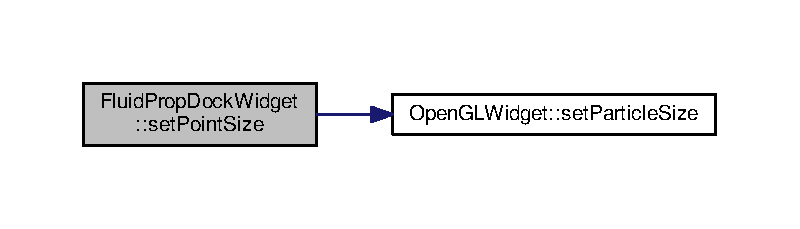
\includegraphics[width=350pt]{class_fluid_prop_dock_widget_afeb4fe68de9245e8fc3696870ed239b1_cgraph}
\end{center}
\end{figure}




Here is the caller graph for this function\-:\nopagebreak
\begin{figure}[H]
\begin{center}
\leavevmode
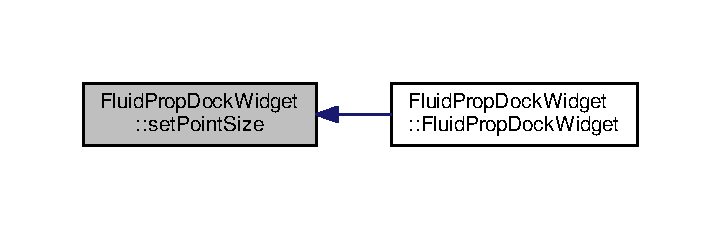
\includegraphics[width=346pt]{class_fluid_prop_dock_widget_afeb4fe68de9245e8fc3696870ed239b1_icgraph}
\end{center}
\end{figure}


\hypertarget{class_fluid_prop_dock_widget_a2f07e4371b46ccbd7c649264e94646de}{\index{Fluid\-Prop\-Dock\-Widget@{Fluid\-Prop\-Dock\-Widget}!set\-Refraction\-Ratio@{set\-Refraction\-Ratio}}
\index{set\-Refraction\-Ratio@{set\-Refraction\-Ratio}!FluidPropDockWidget@{Fluid\-Prop\-Dock\-Widget}}
\subsubsection[{set\-Refraction\-Ratio}]{\setlength{\rightskip}{0pt plus 5cm}void Fluid\-Prop\-Dock\-Widget\-::set\-Refraction\-Ratio (
\begin{DoxyParamCaption}
\item[{double}]{\-\_\-eta}
\end{DoxyParamCaption}
)\hspace{0.3cm}{\ttfamily [inline]}, {\ttfamily [slot]}}}\label{class_fluid_prop_dock_widget_a2f07e4371b46ccbd7c649264e94646de}


slot to set the refraction ratio of our fluid 


\begin{DoxyParams}{Parameters}
{\em \-\_\-eta} & -\/ desired refraction ratio \\
\hline
\end{DoxyParams}


Here is the call graph for this function\-:\nopagebreak
\begin{figure}[H]
\begin{center}
\leavevmode
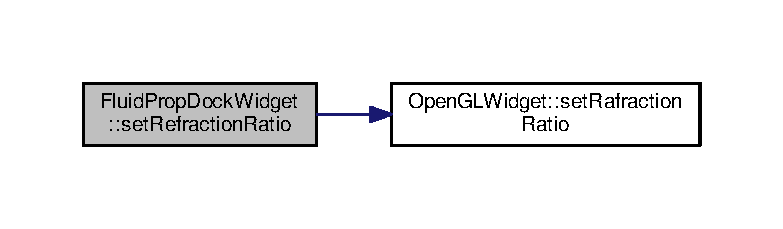
\includegraphics[width=350pt]{class_fluid_prop_dock_widget_a2f07e4371b46ccbd7c649264e94646de_cgraph}
\end{center}
\end{figure}




Here is the caller graph for this function\-:\nopagebreak
\begin{figure}[H]
\begin{center}
\leavevmode
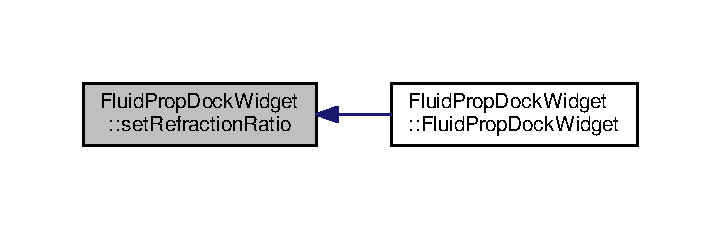
\includegraphics[width=346pt]{class_fluid_prop_dock_widget_a2f07e4371b46ccbd7c649264e94646de_icgraph}
\end{center}
\end{figure}


\hypertarget{class_fluid_prop_dock_widget_a04366783099838b9a2b364ecd3d53da3}{\index{Fluid\-Prop\-Dock\-Widget@{Fluid\-Prop\-Dock\-Widget}!set\-Smoothing\-Length@{set\-Smoothing\-Length}}
\index{set\-Smoothing\-Length@{set\-Smoothing\-Length}!FluidPropDockWidget@{Fluid\-Prop\-Dock\-Widget}}
\subsubsection[{set\-Smoothing\-Length}]{\setlength{\rightskip}{0pt plus 5cm}void Fluid\-Prop\-Dock\-Widget\-::set\-Smoothing\-Length (
\begin{DoxyParamCaption}
\item[{double}]{\-\_\-len}
\end{DoxyParamCaption}
)\hspace{0.3cm}{\ttfamily [inline]}, {\ttfamily [slot]}}}\label{class_fluid_prop_dock_widget_a04366783099838b9a2b364ecd3d53da3}


slot to set the smoothing length of our fluid simulation 


\begin{DoxyParams}{Parameters}
{\em \-\_\-len} & -\/ desired smoothing length of fluid simulation \\
\hline
\end{DoxyParams}


Here is the call graph for this function\-:\nopagebreak
\begin{figure}[H]
\begin{center}
\leavevmode
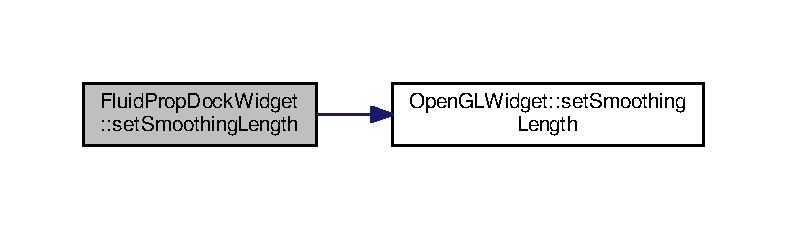
\includegraphics[width=350pt]{class_fluid_prop_dock_widget_a04366783099838b9a2b364ecd3d53da3_cgraph}
\end{center}
\end{figure}




Here is the caller graph for this function\-:\nopagebreak
\begin{figure}[H]
\begin{center}
\leavevmode
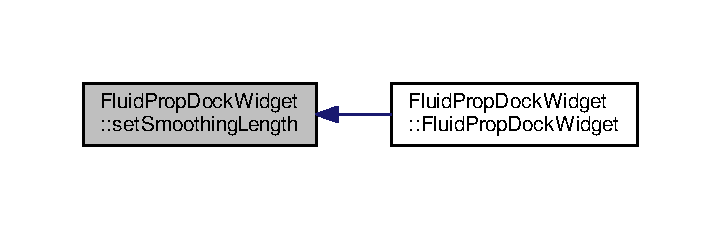
\includegraphics[width=346pt]{class_fluid_prop_dock_widget_a04366783099838b9a2b364ecd3d53da3_icgraph}
\end{center}
\end{figure}


\hypertarget{class_fluid_prop_dock_widget_ae59c72dfb12faf77940e805e94b78cbf}{\index{Fluid\-Prop\-Dock\-Widget@{Fluid\-Prop\-Dock\-Widget}!set\-Spawn\-Box\-Size@{set\-Spawn\-Box\-Size}}
\index{set\-Spawn\-Box\-Size@{set\-Spawn\-Box\-Size}!FluidPropDockWidget@{Fluid\-Prop\-Dock\-Widget}}
\subsubsection[{set\-Spawn\-Box\-Size}]{\setlength{\rightskip}{0pt plus 5cm}void Fluid\-Prop\-Dock\-Widget\-::set\-Spawn\-Box\-Size (
\begin{DoxyParamCaption}
\item[{double}]{\-\_\-size}
\end{DoxyParamCaption}
)\hspace{0.3cm}{\ttfamily [inline]}, {\ttfamily [slot]}}}\label{class_fluid_prop_dock_widget_ae59c72dfb12faf77940e805e94b78cbf}


slot to set the spawn box size 


\begin{DoxyParams}{Parameters}
{\em \-\_\-size} & -\/ desired size of spawn box \\
\hline
\end{DoxyParams}


Here is the call graph for this function\-:\nopagebreak
\begin{figure}[H]
\begin{center}
\leavevmode
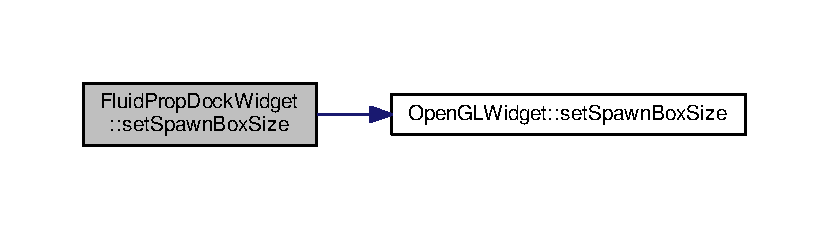
\includegraphics[width=350pt]{class_fluid_prop_dock_widget_ae59c72dfb12faf77940e805e94b78cbf_cgraph}
\end{center}
\end{figure}




Here is the caller graph for this function\-:\nopagebreak
\begin{figure}[H]
\begin{center}
\leavevmode
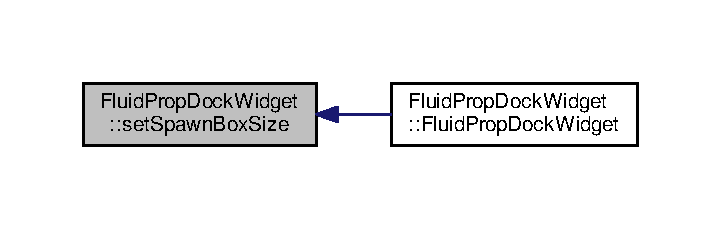
\includegraphics[width=346pt]{class_fluid_prop_dock_widget_ae59c72dfb12faf77940e805e94b78cbf_icgraph}
\end{center}
\end{figure}


\hypertarget{class_fluid_prop_dock_widget_a350d3512b0f415f51ea121e6f1136028}{\index{Fluid\-Prop\-Dock\-Widget@{Fluid\-Prop\-Dock\-Widget}!set\-Thickness@{set\-Thickness}}
\index{set\-Thickness@{set\-Thickness}!FluidPropDockWidget@{Fluid\-Prop\-Dock\-Widget}}
\subsubsection[{set\-Thickness}]{\setlength{\rightskip}{0pt plus 5cm}void Fluid\-Prop\-Dock\-Widget\-::set\-Thickness (
\begin{DoxyParamCaption}
\item[{double}]{\-\_\-thickness}
\end{DoxyParamCaption}
)\hspace{0.3cm}{\ttfamily [inline]}, {\ttfamily [slot]}}}\label{class_fluid_prop_dock_widget_a350d3512b0f415f51ea121e6f1136028}


slot to set the thickness or the particles in our simulation 


\begin{DoxyParams}{Parameters}
{\em \-\_\-thickness} & -\/ desired thickness \\
\hline
\end{DoxyParams}


Here is the call graph for this function\-:\nopagebreak
\begin{figure}[H]
\begin{center}
\leavevmode
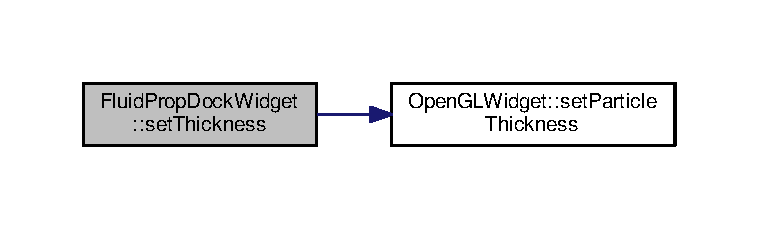
\includegraphics[width=350pt]{class_fluid_prop_dock_widget_a350d3512b0f415f51ea121e6f1136028_cgraph}
\end{center}
\end{figure}




Here is the caller graph for this function\-:\nopagebreak
\begin{figure}[H]
\begin{center}
\leavevmode
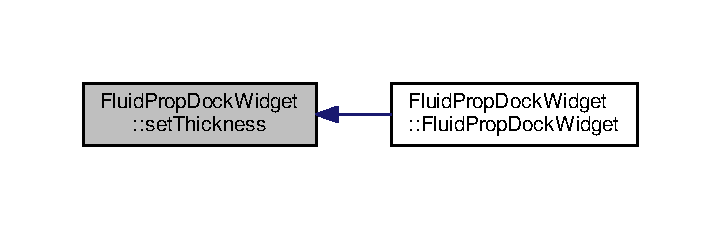
\includegraphics[width=346pt]{class_fluid_prop_dock_widget_a350d3512b0f415f51ea121e6f1136028_icgraph}
\end{center}
\end{figure}


\hypertarget{class_fluid_prop_dock_widget_a03628de74620c25af71461a255163a84}{\index{Fluid\-Prop\-Dock\-Widget@{Fluid\-Prop\-Dock\-Widget}!set\-Time\-Step@{set\-Time\-Step}}
\index{set\-Time\-Step@{set\-Time\-Step}!FluidPropDockWidget@{Fluid\-Prop\-Dock\-Widget}}
\subsubsection[{set\-Time\-Step}]{\setlength{\rightskip}{0pt plus 5cm}void Fluid\-Prop\-Dock\-Widget\-::set\-Time\-Step (
\begin{DoxyParamCaption}
\item[{double}]{\-\_\-step}
\end{DoxyParamCaption}
)\hspace{0.3cm}{\ttfamily [inline]}, {\ttfamily [slot]}}}\label{class_fluid_prop_dock_widget_a03628de74620c25af71461a255163a84}


slot to set the time step our simulation 


\begin{DoxyParams}{Parameters}
{\em \-\_\-step} & -\/ desired time step of simulation \\
\hline
\end{DoxyParams}


Here is the call graph for this function\-:\nopagebreak
\begin{figure}[H]
\begin{center}
\leavevmode
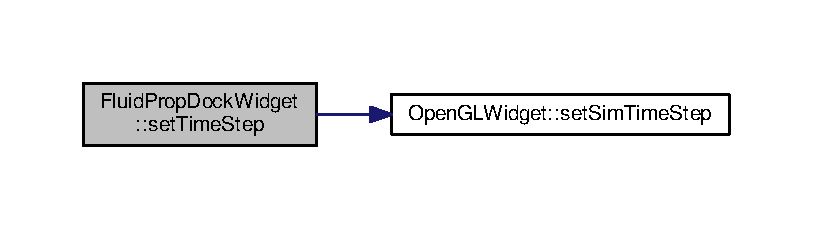
\includegraphics[width=350pt]{class_fluid_prop_dock_widget_a03628de74620c25af71461a255163a84_cgraph}
\end{center}
\end{figure}




Here is the caller graph for this function\-:\nopagebreak
\begin{figure}[H]
\begin{center}
\leavevmode
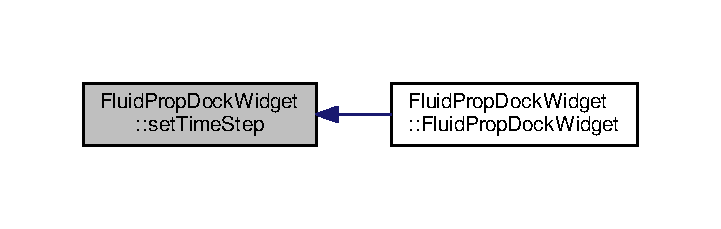
\includegraphics[width=346pt]{class_fluid_prop_dock_widget_a03628de74620c25af71461a255163a84_icgraph}
\end{center}
\end{figure}


\hypertarget{class_fluid_prop_dock_widget_a7c06460036dcca6716dea7b7fc70ad66}{\index{Fluid\-Prop\-Dock\-Widget@{Fluid\-Prop\-Dock\-Widget}!set\-Vel\-Correction@{set\-Vel\-Correction}}
\index{set\-Vel\-Correction@{set\-Vel\-Correction}!FluidPropDockWidget@{Fluid\-Prop\-Dock\-Widget}}
\subsubsection[{set\-Vel\-Correction}]{\setlength{\rightskip}{0pt plus 5cm}void Fluid\-Prop\-Dock\-Widget\-::set\-Vel\-Correction (
\begin{DoxyParamCaption}
\item[{double}]{\-\_\-val}
\end{DoxyParamCaption}
)\hspace{0.3cm}{\ttfamily [inline]}, {\ttfamily [slot]}}}\label{class_fluid_prop_dock_widget_a7c06460036dcca6716dea7b7fc70ad66}


slot to set the velocity correction of our simulatin 

\-\_\-val -\/ value of velocity correciion 

Here is the call graph for this function\-:\nopagebreak
\begin{figure}[H]
\begin{center}
\leavevmode
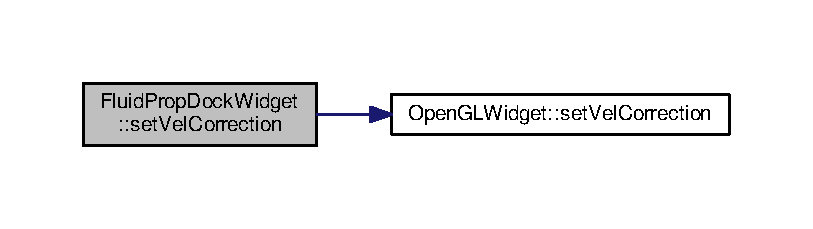
\includegraphics[width=350pt]{class_fluid_prop_dock_widget_a7c06460036dcca6716dea7b7fc70ad66_cgraph}
\end{center}
\end{figure}




Here is the caller graph for this function\-:\nopagebreak
\begin{figure}[H]
\begin{center}
\leavevmode
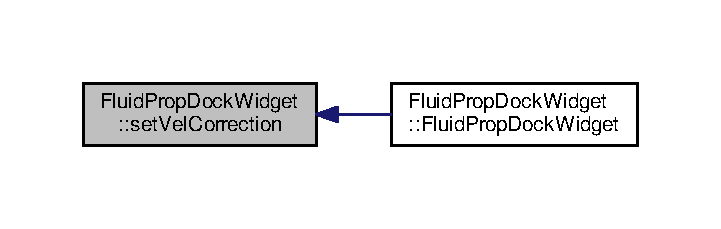
\includegraphics[width=346pt]{class_fluid_prop_dock_widget_a7c06460036dcca6716dea7b7fc70ad66_icgraph}
\end{center}
\end{figure}


\hypertarget{class_fluid_prop_dock_widget_a473ce1156c2ab118e6af5d99ec700764}{\index{Fluid\-Prop\-Dock\-Widget@{Fluid\-Prop\-Dock\-Widget}!set\-Viscosity@{set\-Viscosity}}
\index{set\-Viscosity@{set\-Viscosity}!FluidPropDockWidget@{Fluid\-Prop\-Dock\-Widget}}
\subsubsection[{set\-Viscosity}]{\setlength{\rightskip}{0pt plus 5cm}void Fluid\-Prop\-Dock\-Widget\-::set\-Viscosity (
\begin{DoxyParamCaption}
\item[{double}]{\-\_\-visc}
\end{DoxyParamCaption}
)\hspace{0.3cm}{\ttfamily [inline]}, {\ttfamily [slot]}}}\label{class_fluid_prop_dock_widget_a473ce1156c2ab118e6af5d99ec700764}


slot to set the viscosity coeficient of our fluid 


\begin{DoxyParams}{Parameters}
{\em \-\_\-visc} & -\/ desired viscosity of fluid \\
\hline
\end{DoxyParams}


Here is the call graph for this function\-:\nopagebreak
\begin{figure}[H]
\begin{center}
\leavevmode
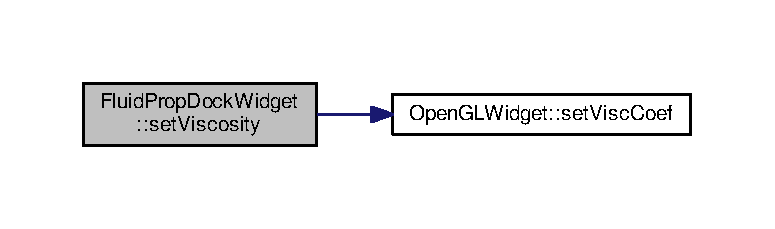
\includegraphics[width=350pt]{class_fluid_prop_dock_widget_a473ce1156c2ab118e6af5d99ec700764_cgraph}
\end{center}
\end{figure}




Here is the caller graph for this function\-:\nopagebreak
\begin{figure}[H]
\begin{center}
\leavevmode
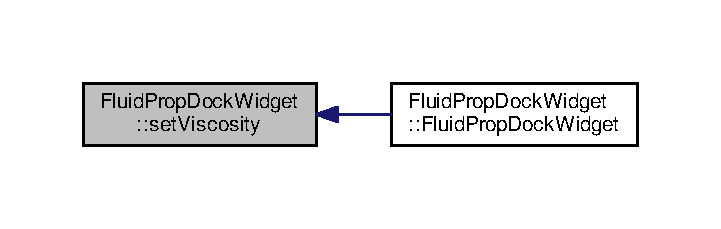
\includegraphics[width=346pt]{class_fluid_prop_dock_widget_a473ce1156c2ab118e6af5d99ec700764_icgraph}
\end{center}
\end{figure}




The documentation for this class was generated from the following files\-:\begin{DoxyCompactItemize}
\item 
/home/dexternation/\-A\-G\-S\-D\-T\-Fluid\-Sim/include/Fluid\-Prop\-Dock\-Widget.\-h\item 
/home/dexternation/\-A\-G\-S\-D\-T\-Fluid\-Sim/src/Fluid\-Prop\-Dock\-Widget.\-cpp\end{DoxyCompactItemize}

\hypertarget{class_fluid_shader}{\section{Fluid\-Shader Class Reference}
\label{class_fluid_shader}\index{Fluid\-Shader@{Fluid\-Shader}}
}


Fluid shader. Method can be found at \href{http://developer.download.nvidia.com/presentations/2010/gdc/Direct3D_Effects.pdf}{\tt http\-://developer.\-download.\-nvidia.\-com/presentations/2010/gdc/\-Direct3\-D\-\_\-\-Effects.\-pdf}.  




{\ttfamily \#include $<$Fluid\-Shader.\-h$>$}



Collaboration diagram for Fluid\-Shader\-:\nopagebreak
\begin{figure}[H]
\begin{center}
\leavevmode
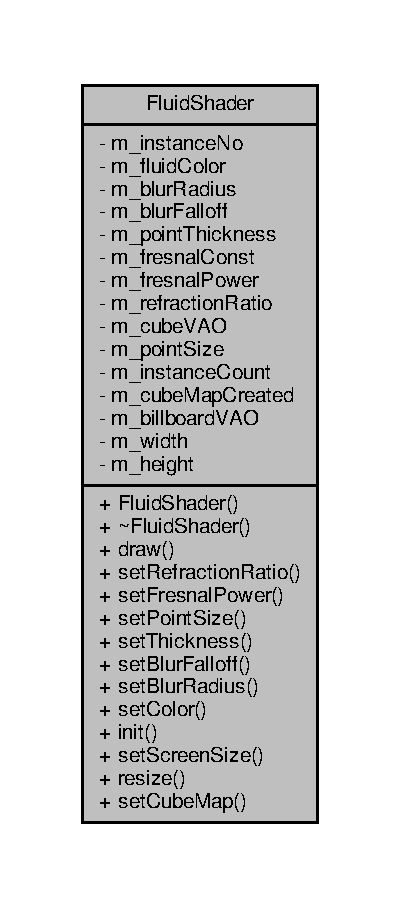
\includegraphics[width=192pt]{class_fluid_shader__coll__graph}
\end{center}
\end{figure}
\subsection*{Public Member Functions}
\begin{DoxyCompactItemize}
\item 
\hyperlink{class_fluid_shader_ad3f76a7573c376b87189c0074d323e19}{Fluid\-Shader} (int \-\_\-width, int \-\_\-height)
\begin{DoxyCompactList}\small\item\em our default constructor that sets up our shader \end{DoxyCompactList}\item 
\hypertarget{class_fluid_shader_a00151325231de231c26c85bde9a7587d}{\hyperlink{class_fluid_shader_a00151325231de231c26c85bde9a7587d}{$\sim$\-Fluid\-Shader} ()}\label{class_fluid_shader_a00151325231de231c26c85bde9a7587d}

\begin{DoxyCompactList}\small\item\em our default destructor \end{DoxyCompactList}\item 
void \hyperlink{class_fluid_shader_ae4a324bbc4f7926bab3d45fb58ba59f6}{draw} (G\-Luint \-\_\-position\-V\-A\-O, int \-\_\-num\-Points, ngl\-::\-Mat4 \-\_\-\-M, ngl\-::\-Mat4 \-\_\-\-V, ngl\-::\-Mat4 \-\_\-\-P, ngl\-::\-Mat4 \-\_\-rot\-M, ngl\-::\-Vec4 \-\_\-eye\-Pos)
\begin{DoxyCompactList}\small\item\em draws input points buffer with our fluid shader \end{DoxyCompactList}\item 
\hypertarget{class_fluid_shader_ae91addca716706b77c3d78df77bf9860}{void \hyperlink{class_fluid_shader_ae91addca716706b77c3d78df77bf9860}{set\-Refraction\-Ratio} (float \-\_\-eta)}\label{class_fluid_shader_ae91addca716706b77c3d78df77bf9860}

\begin{DoxyCompactList}\small\item\em sets our refraction ratio \end{DoxyCompactList}\item 
\hypertarget{class_fluid_shader_ae02755692742b4c8e5fb5ed139709a42}{void \hyperlink{class_fluid_shader_ae02755692742b4c8e5fb5ed139709a42}{set\-Fresnal\-Power} (float \-\_\-power)}\label{class_fluid_shader_ae02755692742b4c8e5fb5ed139709a42}

\begin{DoxyCompactList}\small\item\em mutator for the fresnal power. this effects the reflection of our fluid \end{DoxyCompactList}\item 
void \hyperlink{class_fluid_shader_aa48f21bea9b0fbb456753442f874d10d}{set\-Point\-Size} (float \-\_\-size)
\begin{DoxyCompactList}\small\item\em set how big we want to draw our fluid particles \end{DoxyCompactList}\item 
void \hyperlink{class_fluid_shader_a076afe8aa143ad01ac4fc2a3b9078305}{set\-Thickness} (float \-\_\-thickness)
\begin{DoxyCompactList}\small\item\em set how thick we want to render each particle \end{DoxyCompactList}\item 
void \hyperlink{class_fluid_shader_a5180f954e326d1f70b83efe5fcaea748}{set\-Blur\-Falloff} (float \-\_\-falloff)
\begin{DoxyCompactList}\small\item\em set the blur fall off of our bilateral filter shader \end{DoxyCompactList}\item 
void \hyperlink{class_fluid_shader_ac9b7d6ee1135c3089894e5db3292bd0e}{set\-Blur\-Radius} (float \-\_\-radius)
\begin{DoxyCompactList}\small\item\em set the blur ratius of our bilateral filter shader \end{DoxyCompactList}\item 
void \hyperlink{class_fluid_shader_a21f895c071bf27ba60f780138211c710}{set\-Color} (float \-\_\-col\-R, float \-\_\-col\-G, float \-\_\-col\-B)
\begin{DoxyCompactList}\small\item\em set the desired color of our fluid. Color values from 0-\/1. \end{DoxyCompactList}\item 
\hypertarget{class_fluid_shader_ae719bbf1e465c9cc116682c3e5ac6604}{void \hyperlink{class_fluid_shader_ae719bbf1e465c9cc116682c3e5ac6604}{init} ()}\label{class_fluid_shader_ae719bbf1e465c9cc116682c3e5ac6604}

\begin{DoxyCompactList}\small\item\em creates our shader \end{DoxyCompactList}\end{DoxyCompactItemize}
\subsection*{Static Public Member Functions}
\begin{DoxyCompactItemize}
\item 
static void \hyperlink{class_fluid_shader_a59302f1395ebd10872da9eb9d733d749}{set\-Screen\-Size} (int \-\_\-w, int \-\_\-h)
\begin{DoxyCompactList}\small\item\em informas the shader of the screen size \end{DoxyCompactList}\item 
static void \hyperlink{class_fluid_shader_a46a269869d9c2efa74a8e89d7a8e4960}{resize} (int \-\_\-w, int \-\_\-h)
\begin{DoxyCompactList}\small\item\em resizes our shader output \end{DoxyCompactList}\item 
static void \hyperlink{class_fluid_shader_a1e3a4859b77f0420d2ae201c3f09b5f4}{set\-Cube\-Map} (int \-\_\-width, int \-\_\-height, const G\-Lvoid $\ast$\-\_\-front, const G\-Lvoid $\ast$\-\_\-back, const G\-Lvoid $\ast$\-\_\-top, const G\-Lvoid $\ast$\-\_\-bottom, const G\-Lvoid $\ast$\-\_\-left, const G\-Lvoid $\ast$\-\_\-right)
\begin{DoxyCompactList}\small\item\em sets the shading cube map \end{DoxyCompactList}\end{DoxyCompactItemize}
\subsection*{Private Attributes}
\begin{DoxyCompactItemize}
\item 
\hypertarget{class_fluid_shader_ac5d0650a0b155d50a85c71a97fa92494}{int \hyperlink{class_fluid_shader_ac5d0650a0b155d50a85c71a97fa92494}{m\-\_\-instance\-No}}\label{class_fluid_shader_ac5d0650a0b155d50a85c71a97fa92494}

\begin{DoxyCompactList}\small\item\em the id number of our shader instance \end{DoxyCompactList}\item 
\hypertarget{class_fluid_shader_a33b99afb36290dd90bc54c48b0a88ba4}{ngl\-::\-Vec3 \hyperlink{class_fluid_shader_a33b99afb36290dd90bc54c48b0a88ba4}{m\-\_\-fluid\-Color}}\label{class_fluid_shader_a33b99afb36290dd90bc54c48b0a88ba4}

\begin{DoxyCompactList}\small\item\em our fluid color \end{DoxyCompactList}\item 
\hypertarget{class_fluid_shader_a67b0f8349a22d7ed52f6f2081a4871d1}{float \hyperlink{class_fluid_shader_a67b0f8349a22d7ed52f6f2081a4871d1}{m\-\_\-blur\-Radius}}\label{class_fluid_shader_a67b0f8349a22d7ed52f6f2081a4871d1}

\begin{DoxyCompactList}\small\item\em Bilateral filter blur radius. \end{DoxyCompactList}\item 
\hypertarget{class_fluid_shader_afb00e888a3e963d94d06dd49132e3e42}{float \hyperlink{class_fluid_shader_afb00e888a3e963d94d06dd49132e3e42}{m\-\_\-blur\-Falloff}}\label{class_fluid_shader_afb00e888a3e963d94d06dd49132e3e42}

\begin{DoxyCompactList}\small\item\em Bilateral filter blur falloff. \end{DoxyCompactList}\item 
\hypertarget{class_fluid_shader_ac286b2c5dcc2c68ae69e87f74a4c1efa}{float \hyperlink{class_fluid_shader_ac286b2c5dcc2c68ae69e87f74a4c1efa}{m\-\_\-point\-Thickness}}\label{class_fluid_shader_ac286b2c5dcc2c68ae69e87f74a4c1efa}

\begin{DoxyCompactList}\small\item\em the thickness of our points \end{DoxyCompactList}\item 
\hypertarget{class_fluid_shader_aef86b483692d6e7c8fa5349ef6c53f19}{float \hyperlink{class_fluid_shader_aef86b483692d6e7c8fa5349ef6c53f19}{m\-\_\-fresnal\-Const}}\label{class_fluid_shader_aef86b483692d6e7c8fa5349ef6c53f19}

\begin{DoxyCompactList}\small\item\em fresnal constant \end{DoxyCompactList}\item 
\hypertarget{class_fluid_shader_a7959268c3e8f2371debe83375cc3113c}{float \hyperlink{class_fluid_shader_a7959268c3e8f2371debe83375cc3113c}{m\-\_\-fresnal\-Power}}\label{class_fluid_shader_a7959268c3e8f2371debe83375cc3113c}

\begin{DoxyCompactList}\small\item\em our Fresnal power, this effects our reflection \end{DoxyCompactList}\item 
\hypertarget{class_fluid_shader_a59895f7e705bf3c0c874d61a03e24324}{float \hyperlink{class_fluid_shader_a59895f7e705bf3c0c874d61a03e24324}{m\-\_\-refraction\-Ratio}}\label{class_fluid_shader_a59895f7e705bf3c0c874d61a03e24324}

\begin{DoxyCompactList}\small\item\em our refraction ratio \end{DoxyCompactList}\item 
\hypertarget{class_fluid_shader_a00339308061f3acdd4ae9d2ee019e0c4}{G\-Luint \hyperlink{class_fluid_shader_a00339308061f3acdd4ae9d2ee019e0c4}{m\-\_\-cube\-V\-A\-O}}\label{class_fluid_shader_a00339308061f3acdd4ae9d2ee019e0c4}

\begin{DoxyCompactList}\small\item\em cube V\-A\-O for rendering cube maps \end{DoxyCompactList}\item 
\hypertarget{class_fluid_shader_a93f87bf852746ded66803552309534e6}{float \hyperlink{class_fluid_shader_a93f87bf852746ded66803552309534e6}{m\-\_\-point\-Size}}\label{class_fluid_shader_a93f87bf852746ded66803552309534e6}

\begin{DoxyCompactList}\small\item\em the size to draw our water particles \end{DoxyCompactList}\end{DoxyCompactItemize}
\subsection*{Static Private Attributes}
\begin{DoxyCompactItemize}
\item 
\hypertarget{class_fluid_shader_a7222716799d6097618fce425d1da13fc}{static int \hyperlink{class_fluid_shader_a7222716799d6097618fce425d1da13fc}{m\-\_\-instance\-Count}}\label{class_fluid_shader_a7222716799d6097618fce425d1da13fc}

\begin{DoxyCompactList}\small\item\em static member so we know how many instances of the shader there are \end{DoxyCompactList}\item 
\hypertarget{class_fluid_shader_adeec5576690fb6c4bff765932037e286}{static bool \hyperlink{class_fluid_shader_adeec5576690fb6c4bff765932037e286}{m\-\_\-cube\-Map\-Created}}\label{class_fluid_shader_adeec5576690fb6c4bff765932037e286}

\begin{DoxyCompactList}\small\item\em bool to indicate if our cube map has been loaded in \end{DoxyCompactList}\item 
\hypertarget{class_fluid_shader_ade4ee84f9ee1068e17ba3a0e980aa11b}{static G\-Luint \hyperlink{class_fluid_shader_ade4ee84f9ee1068e17ba3a0e980aa11b}{m\-\_\-billboard\-V\-A\-O}}\label{class_fluid_shader_ade4ee84f9ee1068e17ba3a0e980aa11b}

\begin{DoxyCompactList}\small\item\em billboard V\-A\-O for rendering textures to screen \end{DoxyCompactList}\item 
\hypertarget{class_fluid_shader_aab541db2bd8b6063bb98d4d1d94d8d13}{static int \hyperlink{class_fluid_shader_aab541db2bd8b6063bb98d4d1d94d8d13}{m\-\_\-width}}\label{class_fluid_shader_aab541db2bd8b6063bb98d4d1d94d8d13}

\begin{DoxyCompactList}\small\item\em the width of the screen to shade in \end{DoxyCompactList}\item 
\hypertarget{class_fluid_shader_a85d49ca361e2b85558466c9db1215c24}{static int \hyperlink{class_fluid_shader_a85d49ca361e2b85558466c9db1215c24}{m\-\_\-height}}\label{class_fluid_shader_a85d49ca361e2b85558466c9db1215c24}

\begin{DoxyCompactList}\small\item\em the height of the screen to shade in \end{DoxyCompactList}\end{DoxyCompactItemize}


\subsection{Detailed Description}
Fluid shader. Method can be found at \href{http://developer.download.nvidia.com/presentations/2010/gdc/Direct3D_Effects.pdf}{\tt http\-://developer.\-download.\-nvidia.\-com/presentations/2010/gdc/\-Direct3\-D\-\_\-\-Effects.\-pdf}. 

\begin{DoxyAuthor}{Author}
Declan Russell 
\end{DoxyAuthor}
\begin{DoxyDate}{Date}
28/04/2015 
\end{DoxyDate}
\begin{DoxyVersion}{Version}
1.\-0 
\end{DoxyVersion}


\subsection{Constructor \& Destructor Documentation}
\hypertarget{class_fluid_shader_ad3f76a7573c376b87189c0074d323e19}{\index{Fluid\-Shader@{Fluid\-Shader}!Fluid\-Shader@{Fluid\-Shader}}
\index{Fluid\-Shader@{Fluid\-Shader}!FluidShader@{Fluid\-Shader}}
\subsubsection[{Fluid\-Shader}]{\setlength{\rightskip}{0pt plus 5cm}Fluid\-Shader\-::\-Fluid\-Shader (
\begin{DoxyParamCaption}
\item[{int}]{\-\_\-width, }
\item[{int}]{\-\_\-height}
\end{DoxyParamCaption}
)}}\label{class_fluid_shader_ad3f76a7573c376b87189c0074d323e19}


our default constructor that sets up our shader 


\begin{DoxyParams}{Parameters}
{\em \-\_\-width} & -\/ the width of the window  \-\_\-height -\/ the height of the window \\
\hline
\end{DoxyParams}


Here is the call graph for this function\-:\nopagebreak
\begin{figure}[H]
\begin{center}
\leavevmode
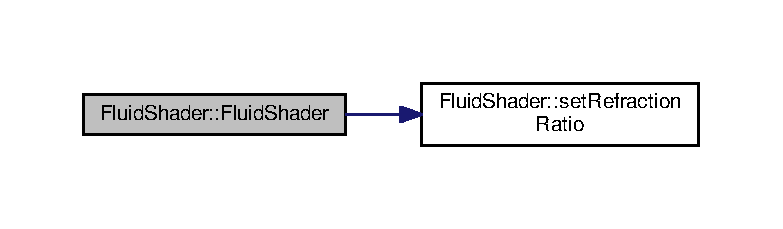
\includegraphics[width=350pt]{class_fluid_shader_ad3f76a7573c376b87189c0074d323e19_cgraph}
\end{center}
\end{figure}




\subsection{Member Function Documentation}
\hypertarget{class_fluid_shader_ae4a324bbc4f7926bab3d45fb58ba59f6}{\index{Fluid\-Shader@{Fluid\-Shader}!draw@{draw}}
\index{draw@{draw}!FluidShader@{Fluid\-Shader}}
\subsubsection[{draw}]{\setlength{\rightskip}{0pt plus 5cm}void Fluid\-Shader\-::draw (
\begin{DoxyParamCaption}
\item[{G\-Luint}]{\-\_\-position\-V\-A\-O, }
\item[{int}]{\-\_\-num\-Points, }
\item[{ngl\-::\-Mat4}]{\-\_\-\-M, }
\item[{ngl\-::\-Mat4}]{\-\_\-\-V, }
\item[{ngl\-::\-Mat4}]{\-\_\-\-P, }
\item[{ngl\-::\-Mat4}]{\-\_\-rot\-M, }
\item[{ngl\-::\-Vec4}]{\-\_\-eye\-Pos}
\end{DoxyParamCaption}
)}}\label{class_fluid_shader_ae4a324bbc4f7926bab3d45fb58ba59f6}


draws input points buffer with our fluid shader 


\begin{DoxyParams}{Parameters}
{\em \-\_\-position\-V\-A\-O} & -\/ V\-A\-O that hold the position data of our particles \\
\hline
{\em \-\_\-num\-Points} & -\/ the number of points to draw \\
\hline
{\em \-\_\-\-M} & -\/ model matrix of our scene \\
\hline
{\em \-\_\-\-V} & -\/ view matrix of our scene \\
\hline
{\em \-\_\-\-P} & -\/ projection matrix of our scene \\
\hline
{\em \-\_\-rot\-M} & -\/ the rotation matrix of our scene to rotate our cube map \\
\hline
{\em \-\_\-eye\-Pos} & -\/ position of the camera in the scene \\
\hline
\end{DoxyParams}


Here is the call graph for this function\-:\nopagebreak
\begin{figure}[H]
\begin{center}
\leavevmode
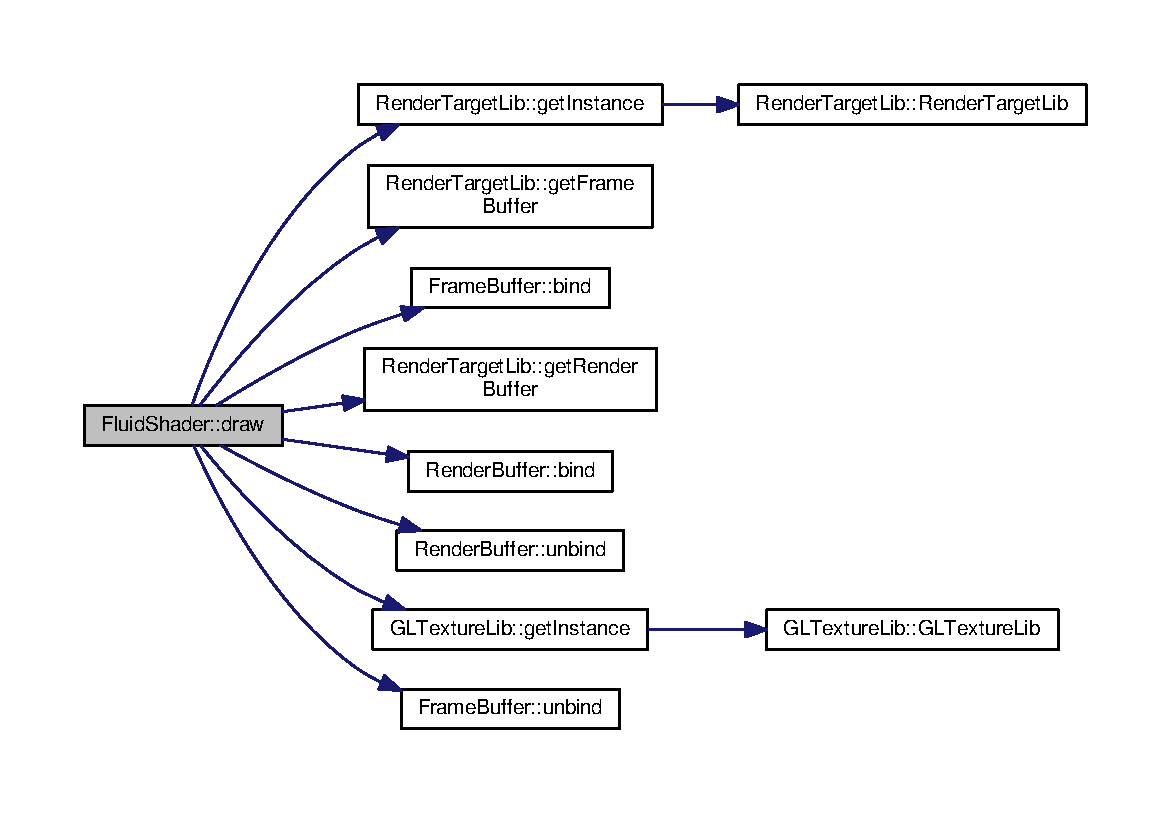
\includegraphics[width=350pt]{class_fluid_shader_ae4a324bbc4f7926bab3d45fb58ba59f6_cgraph}
\end{center}
\end{figure}


\hypertarget{class_fluid_shader_a46a269869d9c2efa74a8e89d7a8e4960}{\index{Fluid\-Shader@{Fluid\-Shader}!resize@{resize}}
\index{resize@{resize}!FluidShader@{Fluid\-Shader}}
\subsubsection[{resize}]{\setlength{\rightskip}{0pt plus 5cm}void Fluid\-Shader\-::resize (
\begin{DoxyParamCaption}
\item[{int}]{\-\_\-w, }
\item[{int}]{\-\_\-h}
\end{DoxyParamCaption}
)\hspace{0.3cm}{\ttfamily [static]}}}\label{class_fluid_shader_a46a269869d9c2efa74a8e89d7a8e4960}


resizes our shader output 

if the screen resizes we need to notify this shader as it uses render targets 
\begin{DoxyParams}{Parameters}
{\em \-\_\-w} & -\/ width to resize \\
\hline
{\em \-\_\-h} & -\/ height to risize \\
\hline
\end{DoxyParams}


Here is the call graph for this function\-:\nopagebreak
\begin{figure}[H]
\begin{center}
\leavevmode
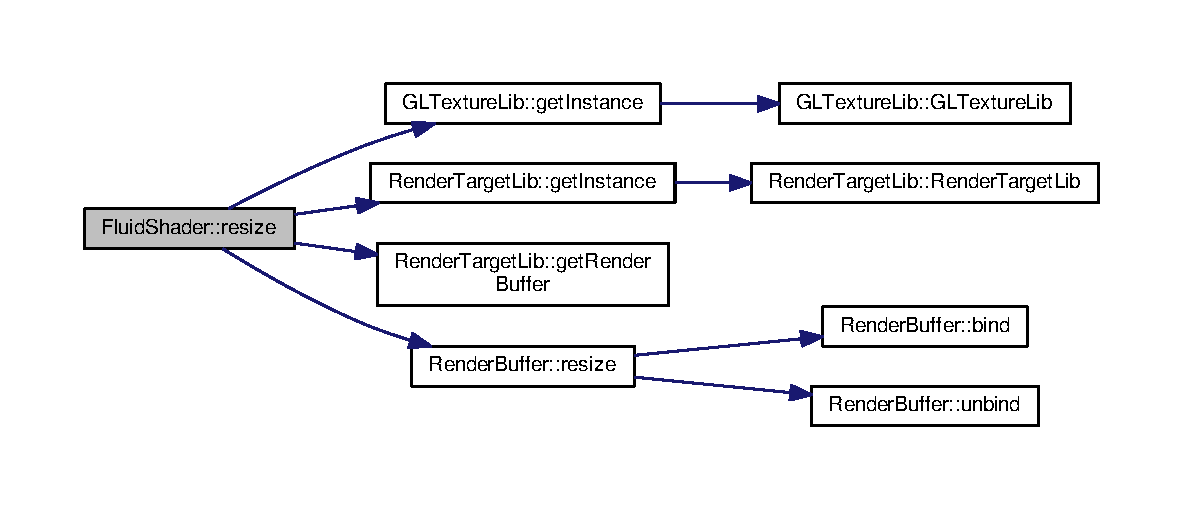
\includegraphics[width=350pt]{class_fluid_shader_a46a269869d9c2efa74a8e89d7a8e4960_cgraph}
\end{center}
\end{figure}


\hypertarget{class_fluid_shader_a5180f954e326d1f70b83efe5fcaea748}{\index{Fluid\-Shader@{Fluid\-Shader}!set\-Blur\-Falloff@{set\-Blur\-Falloff}}
\index{set\-Blur\-Falloff@{set\-Blur\-Falloff}!FluidShader@{Fluid\-Shader}}
\subsubsection[{set\-Blur\-Falloff}]{\setlength{\rightskip}{0pt plus 5cm}void Fluid\-Shader\-::set\-Blur\-Falloff (
\begin{DoxyParamCaption}
\item[{float}]{\-\_\-falloff}
\end{DoxyParamCaption}
)\hspace{0.3cm}{\ttfamily [inline]}}}\label{class_fluid_shader_a5180f954e326d1f70b83efe5fcaea748}


set the blur fall off of our bilateral filter shader 


\begin{DoxyParams}{Parameters}
{\em \-\_\-falloff} & -\/ desired fall off value \\
\hline
\end{DoxyParams}
\hypertarget{class_fluid_shader_ac9b7d6ee1135c3089894e5db3292bd0e}{\index{Fluid\-Shader@{Fluid\-Shader}!set\-Blur\-Radius@{set\-Blur\-Radius}}
\index{set\-Blur\-Radius@{set\-Blur\-Radius}!FluidShader@{Fluid\-Shader}}
\subsubsection[{set\-Blur\-Radius}]{\setlength{\rightskip}{0pt plus 5cm}void Fluid\-Shader\-::set\-Blur\-Radius (
\begin{DoxyParamCaption}
\item[{float}]{\-\_\-radius}
\end{DoxyParamCaption}
)\hspace{0.3cm}{\ttfamily [inline]}}}\label{class_fluid_shader_ac9b7d6ee1135c3089894e5db3292bd0e}


set the blur ratius of our bilateral filter shader 


\begin{DoxyParams}{Parameters}
{\em \-\_\-\-\_\-radius} & -\/ desired blue radius value \\
\hline
\end{DoxyParams}
\hypertarget{class_fluid_shader_a21f895c071bf27ba60f780138211c710}{\index{Fluid\-Shader@{Fluid\-Shader}!set\-Color@{set\-Color}}
\index{set\-Color@{set\-Color}!FluidShader@{Fluid\-Shader}}
\subsubsection[{set\-Color}]{\setlength{\rightskip}{0pt plus 5cm}void Fluid\-Shader\-::set\-Color (
\begin{DoxyParamCaption}
\item[{float}]{\-\_\-col\-R, }
\item[{float}]{\-\_\-col\-G, }
\item[{float}]{\-\_\-col\-B}
\end{DoxyParamCaption}
)\hspace{0.3cm}{\ttfamily [inline]}}}\label{class_fluid_shader_a21f895c071bf27ba60f780138211c710}


set the desired color of our fluid. Color values from 0-\/1. 


\begin{DoxyParams}{Parameters}
{\em \-\_\-col\-R} & -\/ red value \\
\hline
{\em \-\_\-col\-G} & -\/ green value \\
\hline
{\em \-\_\-col\-B} & -\/ blue value \\
\hline
\end{DoxyParams}
\hypertarget{class_fluid_shader_a1e3a4859b77f0420d2ae201c3f09b5f4}{\index{Fluid\-Shader@{Fluid\-Shader}!set\-Cube\-Map@{set\-Cube\-Map}}
\index{set\-Cube\-Map@{set\-Cube\-Map}!FluidShader@{Fluid\-Shader}}
\subsubsection[{set\-Cube\-Map}]{\setlength{\rightskip}{0pt plus 5cm}void Fluid\-Shader\-::set\-Cube\-Map (
\begin{DoxyParamCaption}
\item[{int}]{\-\_\-width, }
\item[{int}]{\-\_\-height, }
\item[{const G\-Lvoid $\ast$}]{\-\_\-front, }
\item[{const G\-Lvoid $\ast$}]{\-\_\-back, }
\item[{const G\-Lvoid $\ast$}]{\-\_\-top, }
\item[{const G\-Lvoid $\ast$}]{\-\_\-bottom, }
\item[{const G\-Lvoid $\ast$}]{\-\_\-left, }
\item[{const G\-Lvoid $\ast$}]{\-\_\-right}
\end{DoxyParamCaption}
)\hspace{0.3cm}{\ttfamily [static]}}}\label{class_fluid_shader_a1e3a4859b77f0420d2ae201c3f09b5f4}


sets the shading cube map 

\-\_\-width -\/ width of our cube map textures \-\_\-height -\/ height of our cube map textures \-\_\-front -\/ front cube map texture \-\_\-back -\/ back cube map texture \-\_\-top -\/ top cube map texture \-\_\-bottom -\/ bottom cube map texture \-\_\-left -\/ left cube map texture \-\_\-right -\/ right cube map texture 

Here is the call graph for this function\-:\nopagebreak
\begin{figure}[H]
\begin{center}
\leavevmode
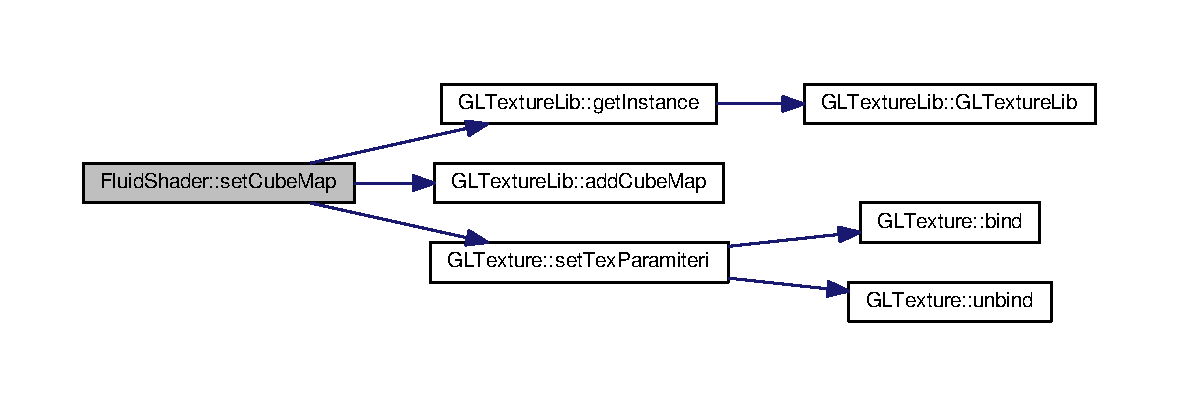
\includegraphics[width=350pt]{class_fluid_shader_a1e3a4859b77f0420d2ae201c3f09b5f4_cgraph}
\end{center}
\end{figure}


\hypertarget{class_fluid_shader_aa48f21bea9b0fbb456753442f874d10d}{\index{Fluid\-Shader@{Fluid\-Shader}!set\-Point\-Size@{set\-Point\-Size}}
\index{set\-Point\-Size@{set\-Point\-Size}!FluidShader@{Fluid\-Shader}}
\subsubsection[{set\-Point\-Size}]{\setlength{\rightskip}{0pt plus 5cm}void Fluid\-Shader\-::set\-Point\-Size (
\begin{DoxyParamCaption}
\item[{float}]{\-\_\-size}
\end{DoxyParamCaption}
)\hspace{0.3cm}{\ttfamily [inline]}}}\label{class_fluid_shader_aa48f21bea9b0fbb456753442f874d10d}


set how big we want to draw our fluid particles 


\begin{DoxyParams}{Parameters}
{\em \-\_\-size} & -\/ desired size \\
\hline
\end{DoxyParams}
\hypertarget{class_fluid_shader_a59302f1395ebd10872da9eb9d733d749}{\index{Fluid\-Shader@{Fluid\-Shader}!set\-Screen\-Size@{set\-Screen\-Size}}
\index{set\-Screen\-Size@{set\-Screen\-Size}!FluidShader@{Fluid\-Shader}}
\subsubsection[{set\-Screen\-Size}]{\setlength{\rightskip}{0pt plus 5cm}static void Fluid\-Shader\-::set\-Screen\-Size (
\begin{DoxyParamCaption}
\item[{int}]{\-\_\-w, }
\item[{int}]{\-\_\-h}
\end{DoxyParamCaption}
)\hspace{0.3cm}{\ttfamily [inline]}, {\ttfamily [static]}}}\label{class_fluid_shader_a59302f1395ebd10872da9eb9d733d749}


informas the shader of the screen size 

\begin{DoxyWarning}{Warning}
This need to be done before you initialise shader 
\end{DoxyWarning}
\hypertarget{class_fluid_shader_a076afe8aa143ad01ac4fc2a3b9078305}{\index{Fluid\-Shader@{Fluid\-Shader}!set\-Thickness@{set\-Thickness}}
\index{set\-Thickness@{set\-Thickness}!FluidShader@{Fluid\-Shader}}
\subsubsection[{set\-Thickness}]{\setlength{\rightskip}{0pt plus 5cm}void Fluid\-Shader\-::set\-Thickness (
\begin{DoxyParamCaption}
\item[{float}]{\-\_\-thickness}
\end{DoxyParamCaption}
)\hspace{0.3cm}{\ttfamily [inline]}}}\label{class_fluid_shader_a076afe8aa143ad01ac4fc2a3b9078305}


set how thick we want to render each particle 


\begin{DoxyParams}{Parameters}
{\em \-\_\-thickness} & -\/ desired thickness \\
\hline
\end{DoxyParams}


The documentation for this class was generated from the following files\-:\begin{DoxyCompactItemize}
\item 
/home/dexternation/\-A\-G\-S\-D\-T\-Fluid\-Sim/include/\hyperlink{_fluid_shader_8h}{Fluid\-Shader.\-h}\item 
/home/dexternation/\-A\-G\-S\-D\-T\-Fluid\-Sim/src/Fluid\-Shader.\-cpp\end{DoxyCompactItemize}

\hypertarget{classfluid_shader_frag}{\section{fluid\-Shader\-Frag Class Reference}
\label{classfluid_shader_frag}\index{fluid\-Shader\-Frag@{fluid\-Shader\-Frag}}
}


Fragment shader to apply the final shading of our fluid. This calculates the fragment normals.  




Collaboration diagram for fluid\-Shader\-Frag\-:\nopagebreak
\begin{figure}[H]
\begin{center}
\leavevmode
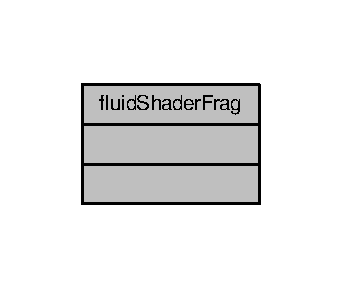
\includegraphics[width=164pt]{classfluid_shader_frag__coll__graph}
\end{center}
\end{figure}


\subsection{Detailed Description}
Fragment shader to apply the final shading of our fluid. This calculates the fragment normals. 

based on a depth pass texture. It also adds reflection and refraction based on a cube map. 

The documentation for this class was generated from the following file\-:\begin{DoxyCompactItemize}
\item 
/home/dexternation/\-A\-G\-S\-D\-T\-Fluid\-Sim/shaders/\hyperlink{fluid_shader_frag_8glsl}{fluid\-Shader\-Frag.\-glsl}\end{DoxyCompactItemize}

\hypertarget{classfluid_shader_vert}{\section{fluid\-Shader\-Vert Class Reference}
\label{classfluid_shader_vert}\index{fluid\-Shader\-Vert@{fluid\-Shader\-Vert}}
}


Vertex shader for our fluid shader. Just passes through positions and tex coords.  




Collaboration diagram for fluid\-Shader\-Vert\-:\nopagebreak
\begin{figure}[H]
\begin{center}
\leavevmode
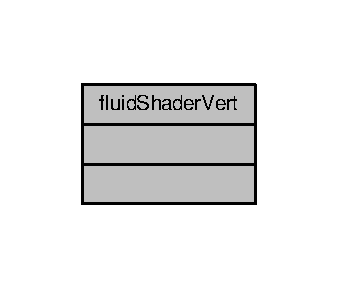
\includegraphics[width=162pt]{classfluid_shader_vert__coll__graph}
\end{center}
\end{figure}


\subsection{Detailed Description}
Vertex shader for our fluid shader. Just passes through positions and tex coords. 

The documentation for this class was generated from the following file\-:\begin{DoxyCompactItemize}
\item 
/home/dexternation/\-A\-G\-S\-D\-T\-Fluid\-Sim/shaders/\hyperlink{fluid_shader_vert_8glsl}{fluid\-Shader\-Vert.\-glsl}\end{DoxyCompactItemize}

\hypertarget{struct_open_g_l_widget_1_1fluid_sim_props}{\section{Open\-G\-L\-Widget\-:\-:fluid\-Sim\-Props Struct Reference}
\label{struct_open_g_l_widget_1_1fluid_sim_props}\index{Open\-G\-L\-Widget\-::fluid\-Sim\-Props@{Open\-G\-L\-Widget\-::fluid\-Sim\-Props}}
}


structure to hold some update information about our fluid simulations  




Collaboration diagram for Open\-G\-L\-Widget\-:\-:fluid\-Sim\-Props\-:\nopagebreak
\begin{figure}[H]
\begin{center}
\leavevmode
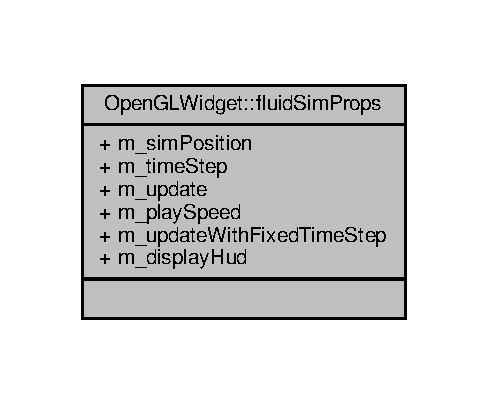
\includegraphics[width=234pt]{struct_open_g_l_widget_1_1fluid_sim_props__coll__graph}
\end{center}
\end{figure}
\subsection*{Public Attributes}
\begin{DoxyCompactItemize}
\item 
\hypertarget{struct_open_g_l_widget_1_1fluid_sim_props_a082f58c5f4d8da41730696d9c8d9f805}{ngl\-::\-Vec3 \hyperlink{struct_open_g_l_widget_1_1fluid_sim_props_a082f58c5f4d8da41730696d9c8d9f805}{m\-\_\-sim\-Position}}\label{struct_open_g_l_widget_1_1fluid_sim_props_a082f58c5f4d8da41730696d9c8d9f805}

\begin{DoxyCompactList}\small\item\em vector of our simulation positions \end{DoxyCompactList}\item 
\hypertarget{struct_open_g_l_widget_1_1fluid_sim_props_a393e95277858fe2f1a15ed8dced0cfa8}{float \hyperlink{struct_open_g_l_widget_1_1fluid_sim_props_a393e95277858fe2f1a15ed8dced0cfa8}{m\-\_\-time\-Step}}\label{struct_open_g_l_widget_1_1fluid_sim_props_a393e95277858fe2f1a15ed8dced0cfa8}

\begin{DoxyCompactList}\small\item\em the timestep to increment ouf simulation \end{DoxyCompactList}\item 
\hypertarget{struct_open_g_l_widget_1_1fluid_sim_props_a61d7eb937176e81210ea734d259a76d1}{bool \hyperlink{struct_open_g_l_widget_1_1fluid_sim_props_a61d7eb937176e81210ea734d259a76d1}{m\-\_\-update}}\label{struct_open_g_l_widget_1_1fluid_sim_props_a61d7eb937176e81210ea734d259a76d1}

\begin{DoxyCompactList}\small\item\em a bool to tell us if we need to update our simulation \end{DoxyCompactList}\item 
\hypertarget{struct_open_g_l_widget_1_1fluid_sim_props_aed3387c3ad2d0e2870b8c0dccbb997c9}{float \hyperlink{struct_open_g_l_widget_1_1fluid_sim_props_aed3387c3ad2d0e2870b8c0dccbb997c9}{m\-\_\-play\-Speed}}\label{struct_open_g_l_widget_1_1fluid_sim_props_aed3387c3ad2d0e2870b8c0dccbb997c9}

\begin{DoxyCompactList}\small\item\em play speed \end{DoxyCompactList}\item 
\hypertarget{struct_open_g_l_widget_1_1fluid_sim_props_ac0da57cf2f1dbf63397abe674fa7c558}{bool \hyperlink{struct_open_g_l_widget_1_1fluid_sim_props_ac0da57cf2f1dbf63397abe674fa7c558}{m\-\_\-update\-With\-Fixed\-Time\-Step}}\label{struct_open_g_l_widget_1_1fluid_sim_props_ac0da57cf2f1dbf63397abe674fa7c558}

\begin{DoxyCompactList}\small\item\em bool to indicate if we want to update with a set time step or with actual time \end{DoxyCompactList}\item 
\hypertarget{struct_open_g_l_widget_1_1fluid_sim_props_a466fa489adaefe2e54cc8ea3b1f64af8}{bool \hyperlink{struct_open_g_l_widget_1_1fluid_sim_props_a466fa489adaefe2e54cc8ea3b1f64af8}{m\-\_\-display\-Hud}}\label{struct_open_g_l_widget_1_1fluid_sim_props_a466fa489adaefe2e54cc8ea3b1f64af8}

\begin{DoxyCompactList}\small\item\em bool to indicate if we want to display the H\-U\-D \end{DoxyCompactList}\end{DoxyCompactItemize}


\subsection{Detailed Description}
structure to hold some update information about our fluid simulations 

The documentation for this struct was generated from the following file\-:\begin{DoxyCompactItemize}
\item 
/home/dexternation/\-A\-G\-S\-D\-T\-Fluid\-Sim/include/\hyperlink{_open_g_l_widget_8h}{Open\-G\-L\-Widget.\-h}\end{DoxyCompactItemize}

\hypertarget{class_frame_buffer}{\section{Frame\-Buffer Class Reference}
\label{class_frame_buffer}\index{Frame\-Buffer@{Frame\-Buffer}}
}


Class for creating frame buffers.  




{\ttfamily \#include $<$Frame\-Buffer.\-h$>$}



Inheritance diagram for Frame\-Buffer\-:


Collaboration diagram for Frame\-Buffer\-:
\subsection*{Public Member Functions}
\begin{DoxyCompactItemize}
\item 
\hypertarget{class_frame_buffer_a6f3763f4551f221b86ca033e2b315c42}{\hyperlink{class_frame_buffer_a6f3763f4551f221b86ca033e2b315c42}{Frame\-Buffer} ()}\label{class_frame_buffer_a6f3763f4551f221b86ca033e2b315c42}

\begin{DoxyCompactList}\small\item\em default constructor to create our frame buffer \end{DoxyCompactList}\item 
\hypertarget{class_frame_buffer_aef8be9884e8cc0fc3f3692e6c6968fa1}{\hyperlink{class_frame_buffer_aef8be9884e8cc0fc3f3692e6c6968fa1}{$\sim$\-Frame\-Buffer} ()}\label{class_frame_buffer_aef8be9884e8cc0fc3f3692e6c6968fa1}

\begin{DoxyCompactList}\small\item\em default destructor removes frambuffers \end{DoxyCompactList}\item 
\hypertarget{class_frame_buffer_a16fa30984714c6070f4c5bde5b5b87f7}{void \hyperlink{class_frame_buffer_a16fa30984714c6070f4c5bde5b5b87f7}{bind} ()}\label{class_frame_buffer_a16fa30984714c6070f4c5bde5b5b87f7}

\begin{DoxyCompactList}\small\item\em bind our frame buffer \end{DoxyCompactList}\item 
\hypertarget{class_frame_buffer_a3b82af89f1c0c0f4c0140e41863256c0}{void \hyperlink{class_frame_buffer_a3b82af89f1c0c0f4c0140e41863256c0}{unbind} ()}\label{class_frame_buffer_a3b82af89f1c0c0f4c0140e41863256c0}

\begin{DoxyCompactList}\small\item\em unbind our frame buffer \end{DoxyCompactList}\item 
\hypertarget{class_frame_buffer_a3acf3a4afec2ebecd93fae3bfba00808}{void \hyperlink{class_frame_buffer_a3acf3a4afec2ebecd93fae3bfba00808}{set\-Frame\-Buffer\-Texture} (G\-Lenum \-\_\-attachment, G\-Luint \-\_\-texture, G\-Lint \-\_\-level)}\label{class_frame_buffer_a3acf3a4afec2ebecd93fae3bfba00808}

\begin{DoxyCompactList}\small\item\em set our frame buffer texture \end{DoxyCompactList}\item 
\hypertarget{class_frame_buffer_a399edc3b7d856ead72e5e04d73223643}{void \hyperlink{class_frame_buffer_a399edc3b7d856ead72e5e04d73223643}{set\-Drawbuffers} (G\-Lsizei \-\_\-n, const G\-Lenum $\ast$\-\_\-bufs)}\label{class_frame_buffer_a399edc3b7d856ead72e5e04d73223643}

\begin{DoxyCompactList}\small\item\em set the draw buffers of our frame buffer \end{DoxyCompactList}\end{DoxyCompactItemize}
\subsection*{Additional Inherited Members}


\subsection{Detailed Description}
Class for creating frame buffers. 

\begin{DoxyAuthor}{Author}
Declan Russell 
\end{DoxyAuthor}
\begin{DoxyDate}{Date}
28/04/2015 
\end{DoxyDate}
\begin{DoxyVersion}{Version}
1.\-0 
\end{DoxyVersion}


The documentation for this class was generated from the following files\-:\begin{DoxyCompactItemize}
\item 
include/\hyperlink{_frame_buffer_8h}{Frame\-Buffer.\-h}\item 
src/Frame\-Buffer.\-cpp\end{DoxyCompactItemize}

\hypertarget{class_g_l_texture}{\section{G\-L\-Texture Class Reference}
\label{class_g_l_texture}\index{G\-L\-Texture@{G\-L\-Texture}}
}


Inheritance diagram for G\-L\-Texture\-:\nopagebreak
\begin{figure}[H]
\begin{center}
\leavevmode
\includegraphics[width=216pt]{class_g_l_texture__inherit__graph}
\end{center}
\end{figure}


Collaboration diagram for G\-L\-Texture\-:\nopagebreak
\begin{figure}[H]
\begin{center}
\leavevmode
\includegraphics[width=216pt]{class_g_l_texture__coll__graph}
\end{center}
\end{figure}
\subsection*{Public Member Functions}
\begin{DoxyCompactItemize}
\item 
\hyperlink{class_g_l_texture_a1f0c33b32b1e37985976b6f10c2263c3}{G\-L\-Texture} (G\-Lenum \-\_\-target, G\-Lint \-\_\-level, G\-Lint \-\_\-internal\-Format, G\-Lsizei \-\_\-width, G\-Lsizei \-\_\-height, G\-Lint \-\_\-border, G\-Lenum \-\_\-format, G\-Lenum \-\_\-type, const G\-Lvoid $\ast$\-\_\-data)
\begin{DoxyCompactList}\small\item\em Constructor that creates our texture on our G\-P\-U. \end{DoxyCompactList}\item 
\hyperlink{class_g_l_texture_a0ec835c5a25261ce08b43b7a1601fc8f}{G\-L\-Texture} (G\-Lenum \-\_\-target, G\-Lint \-\_\-level, G\-Lint \-\_\-internal\-Format, G\-Lsizei \-\_\-width, G\-Lsizei \-\_\-height, G\-Lint \-\_\-border, G\-Lenum \-\_\-format, G\-Lenum \-\_\-type, const G\-Lvoid $\ast$\-\_\-front, const G\-Lvoid $\ast$\-\_\-back, const G\-Lvoid $\ast$\-\_\-top, const G\-Lvoid $\ast$\-\_\-bottom, const G\-Lvoid $\ast$\-\_\-left, const G\-Lvoid $\ast$\-\_\-right)
\begin{DoxyCompactList}\small\item\em Constructor that creates a cube map texture on our G\-P\-U. \end{DoxyCompactList}\item 
\hypertarget{class_g_l_texture_a7a0f04b3bd68c77588c0aea9b30b08c4}{\hyperlink{class_g_l_texture_a7a0f04b3bd68c77588c0aea9b30b08c4}{$\sim$\-G\-L\-Texture} ()}\label{class_g_l_texture_a7a0f04b3bd68c77588c0aea9b30b08c4}

\begin{DoxyCompactList}\small\item\em our destrutor that removes our texture \end{DoxyCompactList}\item 
\hypertarget{class_g_l_texture_add43b53521541bad76faec1cc5292048}{void \hyperlink{class_g_l_texture_add43b53521541bad76faec1cc5292048}{set\-Tex\-Paramiteri} (G\-Lenum \-\_\-pname, G\-Lint \-\_\-param)}\label{class_g_l_texture_add43b53521541bad76faec1cc5292048}

\begin{DoxyCompactList}\small\item\em set our texture integer paramiters same as gl\-Tex\-Paramiteri see Open\-G\-L documentation for more info \end{DoxyCompactList}\item 
\hypertarget{class_g_l_texture_a2a2d0c69601ba7843dd33def3f0d28a2}{void \hyperlink{class_g_l_texture_a2a2d0c69601ba7843dd33def3f0d28a2}{set\-Tex\-Paramiterf} (G\-Lenum \-\_\-pname, G\-Lfloat \-\_\-param)}\label{class_g_l_texture_a2a2d0c69601ba7843dd33def3f0d28a2}

\begin{DoxyCompactList}\small\item\em set our texture float paramiters same as gl\-Tex\-Paramiterf see Open\-G\-L documentation for more info \end{DoxyCompactList}\item 
void \hyperlink{class_g_l_texture_a5b70c5df1d184c9be005b0ed05f1e808}{resize} (G\-Lsizei \-\_\-width, G\-Lsizei \-\_\-height=0)
\begin{DoxyCompactList}\small\item\em resizes our texture \end{DoxyCompactList}\item 
void \hyperlink{class_g_l_texture_a9214dfefb40db4fbb7450bcc0ba70b61}{set\-Data} (const G\-Lvoid $\ast$\-\_\-data, G\-Lsizei \-\_\-width=-\/1, G\-Lsizei \-\_\-height=-\/1)
\begin{DoxyCompactList}\small\item\em set the data of our textue \end{DoxyCompactList}\item 
\hypertarget{class_g_l_texture_af20871f52b9705409078558a33a2c73d}{void \hyperlink{class_g_l_texture_af20871f52b9705409078558a33a2c73d}{set\-Data} (const G\-Lvoid $\ast$\-\_\-front, const G\-Lvoid $\ast$\-\_\-back, const G\-Lvoid $\ast$\-\_\-top, const G\-Lvoid $\ast$\-\_\-bottom, const G\-Lvoid $\ast$\-\_\-left, const G\-Lvoid $\ast$\-\_\-right, G\-Lsizei \-\_\-width=-\/1, G\-Lsizei \-\_\-height=-\/1)}\label{class_g_l_texture_af20871f52b9705409078558a33a2c73d}

\begin{DoxyCompactList}\small\item\em set the data for a cube map texture \end{DoxyCompactList}\item 
void \hyperlink{class_g_l_texture_a8fcf4e5253bccd04ffe6e65af228dabc}{bind} (unsigned int \-\_\-loc)
\begin{DoxyCompactList}\small\item\em binds our texture and set active texture \end{DoxyCompactList}\item 
\hypertarget{class_g_l_texture_a3d26fc3a017fd2079ab67e422f9bac10}{void \hyperlink{class_g_l_texture_a3d26fc3a017fd2079ab67e422f9bac10}{bind} ()}\label{class_g_l_texture_a3d26fc3a017fd2079ab67e422f9bac10}

\begin{DoxyCompactList}\small\item\em binds our texture \end{DoxyCompactList}\item 
\hypertarget{class_g_l_texture_a96090b31b8d550a50eb1d4bed1055774}{void \hyperlink{class_g_l_texture_a96090b31b8d550a50eb1d4bed1055774}{unbind} ()}\label{class_g_l_texture_a96090b31b8d550a50eb1d4bed1055774}

\begin{DoxyCompactList}\small\item\em unbinds our texture \end{DoxyCompactList}\item 
\hypertarget{class_g_l_texture_a0232aa38a299d2570a06367cd8ebd688}{G\-Luint \hyperlink{class_g_l_texture_a0232aa38a299d2570a06367cd8ebd688}{get\-Handle} ()}\label{class_g_l_texture_a0232aa38a299d2570a06367cd8ebd688}

\begin{DoxyCompactList}\small\item\em accessor to the handle of our texture \end{DoxyCompactList}\end{DoxyCompactItemize}
\subsection*{Private Member Functions}
\begin{DoxyCompactItemize}
\item 
\hypertarget{class_g_l_texture_abb3da94e96ea6893e33e51c5422a42f9}{\hyperlink{class_g_l_texture_abb3da94e96ea6893e33e51c5422a42f9}{G\-L\-Texture} ()}\label{class_g_l_texture_abb3da94e96ea6893e33e51c5422a42f9}

\begin{DoxyCompactList}\small\item\em default construtor never to be used. \end{DoxyCompactList}\end{DoxyCompactItemize}
\subsection*{Private Attributes}
\begin{DoxyCompactItemize}
\item 
\hypertarget{class_g_l_texture_afd2e590d7242b2ab54d0ac1473ada6cb}{bool \hyperlink{class_g_l_texture_afd2e590d7242b2ab54d0ac1473ada6cb}{m\-\_\-is\-Cube\-Map}}\label{class_g_l_texture_afd2e590d7242b2ab54d0ac1473ada6cb}

\begin{DoxyCompactList}\small\item\em bool to define if our texture is a cube map \end{DoxyCompactList}\item 
\hypertarget{class_g_l_texture_a7add2254b205660a18801f3e9df6d2b9}{G\-Lint \hyperlink{class_g_l_texture_a7add2254b205660a18801f3e9df6d2b9}{m\-\_\-level}}\label{class_g_l_texture_a7add2254b205660a18801f3e9df6d2b9}

\begin{DoxyCompactList}\small\item\em L\-O\-D detail number. \end{DoxyCompactList}\item 
\hypertarget{class_g_l_texture_a1298a4da5241c3f08188a91efdc820a3}{G\-Lint \hyperlink{class_g_l_texture_a1298a4da5241c3f08188a91efdc820a3}{m\-\_\-internal\-Format}}\label{class_g_l_texture_a1298a4da5241c3f08188a91efdc820a3}

\begin{DoxyCompactList}\small\item\em internal format \end{DoxyCompactList}\item 
\hypertarget{class_g_l_texture_ae2f00682c8694bd9ba1d348363f115f4}{G\-Lsizei \hyperlink{class_g_l_texture_ae2f00682c8694bd9ba1d348363f115f4}{m\-\_\-width}}\label{class_g_l_texture_ae2f00682c8694bd9ba1d348363f115f4}

\begin{DoxyCompactList}\small\item\em width of our texture \end{DoxyCompactList}\item 
\hypertarget{class_g_l_texture_a5148727b47ef344338fad34d8ae9c06c}{G\-Lsizei \hyperlink{class_g_l_texture_a5148727b47ef344338fad34d8ae9c06c}{m\-\_\-height}}\label{class_g_l_texture_a5148727b47ef344338fad34d8ae9c06c}

\begin{DoxyCompactList}\small\item\em height of our texture \end{DoxyCompactList}\item 
\hypertarget{class_g_l_texture_a3a568e28bbc01e1adb7cf33f6889bce5}{G\-Lint \hyperlink{class_g_l_texture_a3a568e28bbc01e1adb7cf33f6889bce5}{m\-\_\-border}}\label{class_g_l_texture_a3a568e28bbc01e1adb7cf33f6889bce5}

\begin{DoxyCompactList}\small\item\em border size of our texture \end{DoxyCompactList}\item 
\hypertarget{class_g_l_texture_af2812d7eebea9c63a59e2994a745e8d0}{G\-Lenum \hyperlink{class_g_l_texture_af2812d7eebea9c63a59e2994a745e8d0}{m\-\_\-format}}\label{class_g_l_texture_af2812d7eebea9c63a59e2994a745e8d0}

\begin{DoxyCompactList}\small\item\em format of our texture \end{DoxyCompactList}\item 
\hypertarget{class_g_l_texture_a1f9a5c5d3ed73c2b2ad6be52967fd883}{G\-Lenum \hyperlink{class_g_l_texture_a1f9a5c5d3ed73c2b2ad6be52967fd883}{m\-\_\-type}}\label{class_g_l_texture_a1f9a5c5d3ed73c2b2ad6be52967fd883}

\begin{DoxyCompactList}\small\item\em type of pixel data \end{DoxyCompactList}\end{DoxyCompactItemize}
\subsection*{Additional Inherited Members}


\subsection{Constructor \& Destructor Documentation}
\hypertarget{class_g_l_texture_a1f0c33b32b1e37985976b6f10c2263c3}{\index{G\-L\-Texture@{G\-L\-Texture}!G\-L\-Texture@{G\-L\-Texture}}
\index{G\-L\-Texture@{G\-L\-Texture}!GLTexture@{G\-L\-Texture}}
\subsubsection[{G\-L\-Texture}]{\setlength{\rightskip}{0pt plus 5cm}G\-L\-Texture\-::\-G\-L\-Texture (
\begin{DoxyParamCaption}
\item[{G\-Lenum}]{\-\_\-target, }
\item[{G\-Lint}]{\-\_\-level, }
\item[{G\-Lint}]{\-\_\-internal\-Format, }
\item[{G\-Lsizei}]{\-\_\-width, }
\item[{G\-Lsizei}]{\-\_\-height, }
\item[{G\-Lint}]{\-\_\-border, }
\item[{G\-Lenum}]{\-\_\-format, }
\item[{G\-Lenum}]{\-\_\-type, }
\item[{const G\-Lvoid $\ast$}]{\-\_\-data}
\end{DoxyParamCaption}
)}}\label{class_g_l_texture_a1f0c33b32b1e37985976b6f10c2263c3}


Constructor that creates our texture on our G\-P\-U. 

See Open\-G\-L documentation for detail about texture paramiters 

Here is the call graph for this function\-:\nopagebreak
\begin{figure}[H]
\begin{center}
\leavevmode
\includegraphics[width=328pt]{class_g_l_texture_a1f0c33b32b1e37985976b6f10c2263c3_cgraph}
\end{center}
\end{figure}


\hypertarget{class_g_l_texture_a0ec835c5a25261ce08b43b7a1601fc8f}{\index{G\-L\-Texture@{G\-L\-Texture}!G\-L\-Texture@{G\-L\-Texture}}
\index{G\-L\-Texture@{G\-L\-Texture}!GLTexture@{G\-L\-Texture}}
\subsubsection[{G\-L\-Texture}]{\setlength{\rightskip}{0pt plus 5cm}G\-L\-Texture\-::\-G\-L\-Texture (
\begin{DoxyParamCaption}
\item[{G\-Lenum}]{\-\_\-target, }
\item[{G\-Lint}]{\-\_\-level, }
\item[{G\-Lint}]{\-\_\-internal\-Format, }
\item[{G\-Lsizei}]{\-\_\-width, }
\item[{G\-Lsizei}]{\-\_\-height, }
\item[{G\-Lint}]{\-\_\-border, }
\item[{G\-Lenum}]{\-\_\-format, }
\item[{G\-Lenum}]{\-\_\-type, }
\item[{const G\-Lvoid $\ast$}]{\-\_\-front, }
\item[{const G\-Lvoid $\ast$}]{\-\_\-back, }
\item[{const G\-Lvoid $\ast$}]{\-\_\-top, }
\item[{const G\-Lvoid $\ast$}]{\-\_\-bottom, }
\item[{const G\-Lvoid $\ast$}]{\-\_\-left, }
\item[{const G\-Lvoid $\ast$}]{\-\_\-right}
\end{DoxyParamCaption}
)}}\label{class_g_l_texture_a0ec835c5a25261ce08b43b7a1601fc8f}


Constructor that creates a cube map texture on our G\-P\-U. 

See Open\-G\-L documentation for detail about texture paramiters 

Here is the call graph for this function\-:\nopagebreak
\begin{figure}[H]
\begin{center}
\leavevmode
\includegraphics[width=328pt]{class_g_l_texture_a0ec835c5a25261ce08b43b7a1601fc8f_cgraph}
\end{center}
\end{figure}




\subsection{Member Function Documentation}
\hypertarget{class_g_l_texture_a8fcf4e5253bccd04ffe6e65af228dabc}{\index{G\-L\-Texture@{G\-L\-Texture}!bind@{bind}}
\index{bind@{bind}!GLTexture@{G\-L\-Texture}}
\subsubsection[{bind}]{\setlength{\rightskip}{0pt plus 5cm}void G\-L\-Texture\-::bind (
\begin{DoxyParamCaption}
\item[{unsigned int}]{\-\_\-loc}
\end{DoxyParamCaption}
)}}\label{class_g_l_texture_a8fcf4e5253bccd04ffe6e65af228dabc}


binds our texture and set active texture 


\begin{DoxyParams}{Parameters}
{\em \-\_\-loc} & -\/ active texture location to bind to \\
\hline
\end{DoxyParams}
\hypertarget{class_g_l_texture_a5b70c5df1d184c9be005b0ed05f1e808}{\index{G\-L\-Texture@{G\-L\-Texture}!resize@{resize}}
\index{resize@{resize}!GLTexture@{G\-L\-Texture}}
\subsubsection[{resize}]{\setlength{\rightskip}{0pt plus 5cm}void G\-L\-Texture\-::resize (
\begin{DoxyParamCaption}
\item[{G\-Lsizei}]{\-\_\-width, }
\item[{G\-Lsizei}]{\-\_\-height = {\ttfamily 0}}
\end{DoxyParamCaption}
)}}\label{class_g_l_texture_a5b70c5df1d184c9be005b0ed05f1e808}


resizes our texture 


\begin{DoxyParams}{Parameters}
{\em \-\_\-width} & -\/ width to resize texture \\
\hline
{\em \-\_\-height} & -\/ height to resize texture \\
\hline
\end{DoxyParams}


Here is the call graph for this function\-:\nopagebreak
\begin{figure}[H]
\begin{center}
\leavevmode
\includegraphics[width=310pt]{class_g_l_texture_a5b70c5df1d184c9be005b0ed05f1e808_cgraph}
\end{center}
\end{figure}


\hypertarget{class_g_l_texture_a9214dfefb40db4fbb7450bcc0ba70b61}{\index{G\-L\-Texture@{G\-L\-Texture}!set\-Data@{set\-Data}}
\index{set\-Data@{set\-Data}!GLTexture@{G\-L\-Texture}}
\subsubsection[{set\-Data}]{\setlength{\rightskip}{0pt plus 5cm}void G\-L\-Texture\-::set\-Data (
\begin{DoxyParamCaption}
\item[{const G\-Lvoid $\ast$}]{\-\_\-data, }
\item[{G\-Lsizei}]{\-\_\-width = {\ttfamily -\/1}, }
\item[{G\-Lsizei}]{\-\_\-height = {\ttfamily -\/1}}
\end{DoxyParamCaption}
)}}\label{class_g_l_texture_a9214dfefb40db4fbb7450bcc0ba70b61}


set the data of our textue 


\begin{DoxyParams}{Parameters}
{\em \-\_\-data} & -\/ data to set to texture \\
\hline
\end{DoxyParams}


Here is the call graph for this function\-:\nopagebreak
\begin{figure}[H]
\begin{center}
\leavevmode
\includegraphics[width=318pt]{class_g_l_texture_a9214dfefb40db4fbb7450bcc0ba70b61_cgraph}
\end{center}
\end{figure}




The documentation for this class was generated from the following files\-:\begin{DoxyCompactItemize}
\item 
/home/dexternation/\-A\-G\-S\-D\-T\-Fluid\-Sim/include/\hyperlink{_g_l_texture_8h}{G\-L\-Texture.\-h}\item 
/home/dexternation/\-A\-G\-S\-D\-T\-Fluid\-Sim/src/G\-L\-Texture.\-cpp\end{DoxyCompactItemize}

\hypertarget{class_g_l_texture_lib}{\section{G\-L\-Texture\-Lib Class Reference}
\label{class_g_l_texture_lib}\index{G\-L\-Texture\-Lib@{G\-L\-Texture\-Lib}}
}


Simple class for loading in and managing Open\-G\-L textures.  




{\ttfamily \#include $<$G\-L\-Texture.\-h$>$}



Collaboration diagram for G\-L\-Texture\-Lib\-:
\subsection*{Public Member Functions}
\begin{DoxyCompactItemize}
\item 
\hyperlink{class_g_l_texture}{G\-L\-Texture} $\ast$ \hyperlink{class_g_l_texture_lib_a778cde3734906f46649defdda30d7d7e}{add\-Texture} (std\-::string \-\_\-name, G\-Lenum \-\_\-target, G\-Lint \-\_\-level, G\-Lint \-\_\-internal\-Format, G\-Lsizei \-\_\-width, G\-Lsizei \-\_\-height, G\-Lint \-\_\-border, G\-Lenum \-\_\-format, G\-Lenum \-\_\-type, const G\-Lvoid $\ast$\-\_\-data)
\begin{DoxyCompactList}\small\item\em add a texture to our texture library \end{DoxyCompactList}\item 
\hyperlink{class_g_l_texture}{G\-L\-Texture} $\ast$ \hyperlink{class_g_l_texture_lib_aece253fdd6aad02adca2d743c463a9f2}{add\-Cube\-Map} (std\-::string \-\_\-name, G\-Lenum \-\_\-target, G\-Lint \-\_\-level, G\-Lint \-\_\-internal\-Format, G\-Lsizei \-\_\-width, G\-Lsizei \-\_\-height, G\-Lint \-\_\-border, G\-Lenum \-\_\-format, G\-Lenum \-\_\-type, const G\-Lvoid $\ast$\-\_\-front, const G\-Lvoid $\ast$\-\_\-back, const G\-Lvoid $\ast$\-\_\-top, const G\-Lvoid $\ast$\-\_\-bottom, const G\-Lvoid $\ast$\-\_\-left, const G\-Lvoid $\ast$\-\_\-right)
\begin{DoxyCompactList}\small\item\em add a cube map to our texture library \end{DoxyCompactList}\item 
\hypertarget{class_g_l_texture_lib_aa18a039ee29d50ccd34a7e1f7d24ce5b}{\hyperlink{class_g_l_texture}{G\-L\-Texture} $\ast$ \hyperlink{class_g_l_texture_lib_aa18a039ee29d50ccd34a7e1f7d24ce5b}{operator\mbox{[}$\,$\mbox{]}} (const std\-::string \&\-\_\-name)}\label{class_g_l_texture_lib_aa18a039ee29d50ccd34a7e1f7d24ce5b}

\begin{DoxyCompactList}\small\item\em overloaded operators to access a texture in our library \end{DoxyCompactList}\item 
\hypertarget{class_g_l_texture_lib_ab4ab9d6def1eb2acecfbe062686ab98e}{\hyperlink{class_g_l_texture}{G\-L\-Texture} $\ast$ \hyperlink{class_g_l_texture_lib_ab4ab9d6def1eb2acecfbe062686ab98e}{operator\mbox{[}$\,$\mbox{]}} (const char $\ast$\-\_\-name)}\label{class_g_l_texture_lib_ab4ab9d6def1eb2acecfbe062686ab98e}

\begin{DoxyCompactList}\small\item\em overloaded operators to access a texture in our library \end{DoxyCompactList}\item 
\hypertarget{class_g_l_texture_lib_aca4b2bd67c1af5b5c1ea304fe2622eac}{\hyperlink{class_g_l_texture_lib_aca4b2bd67c1af5b5c1ea304fe2622eac}{$\sim$\-G\-L\-Texture\-Lib} ()}\label{class_g_l_texture_lib_aca4b2bd67c1af5b5c1ea304fe2622eac}

\begin{DoxyCompactList}\small\item\em our destructor. Removes all textures from library \end{DoxyCompactList}\item 
\hypertarget{class_g_l_texture_lib_a49ba9410297b15f1f2988369853c108f}{void \hyperlink{class_g_l_texture_lib_a49ba9410297b15f1f2988369853c108f}{destroy} ()}\label{class_g_l_texture_lib_a49ba9410297b15f1f2988369853c108f}

\begin{DoxyCompactList}\small\item\em Deletes our library. \end{DoxyCompactList}\end{DoxyCompactItemize}
\subsection*{Static Public Member Functions}
\begin{DoxyCompactItemize}
\item 
\hypertarget{class_g_l_texture_lib_aedb1360fe37f369eb290f773dbada309}{static \hyperlink{class_g_l_texture_lib}{G\-L\-Texture\-Lib} $\ast$ \hyperlink{class_g_l_texture_lib_aedb1360fe37f369eb290f773dbada309}{get\-Instance} ()}\label{class_g_l_texture_lib_aedb1360fe37f369eb290f773dbada309}

\begin{DoxyCompactList}\small\item\em returns an instance of our texture library \end{DoxyCompactList}\end{DoxyCompactItemize}
\subsection*{Private Member Functions}
\begin{DoxyCompactItemize}
\item 
\hypertarget{class_g_l_texture_lib_a7ac1f52801de2e75472f3bd495c40185}{\hyperlink{class_g_l_texture_lib_a7ac1f52801de2e75472f3bd495c40185}{G\-L\-Texture\-Lib} ()}\label{class_g_l_texture_lib_a7ac1f52801de2e75472f3bd495c40185}

\begin{DoxyCompactList}\small\item\em our default constructor. Don't want this to be accessable as this is a singleton class \end{DoxyCompactList}\end{DoxyCompactItemize}
\subsection*{Private Attributes}
\begin{DoxyCompactItemize}
\item 
\hypertarget{class_g_l_texture_lib_a148bbba73a37d5478e1f037699f51d94}{\hyperlink{class_g_l_texture}{G\-L\-Texture} $\ast$ \hyperlink{class_g_l_texture_lib_a148bbba73a37d5478e1f037699f51d94}{m\-\_\-current\-Texture}}\label{class_g_l_texture_lib_a148bbba73a37d5478e1f037699f51d94}

\begin{DoxyCompactList}\small\item\em the current texture in use \end{DoxyCompactList}\item 
\hypertarget{class_g_l_texture_lib_a931a6e49b5a86564de11359436dfb745}{std\-::string \hyperlink{class_g_l_texture_lib_a931a6e49b5a86564de11359436dfb745}{m\-\_\-current\-Texture\-Name}}\label{class_g_l_texture_lib_a931a6e49b5a86564de11359436dfb745}

\begin{DoxyCompactList}\small\item\em the current texture in use name \end{DoxyCompactList}\item 
\hypertarget{class_g_l_texture_lib_adbacf6d620b239b381e955ef4277a6a6}{std\-::map$<$ std\-::string, \\*
\hyperlink{class_g_l_texture}{G\-L\-Texture} $\ast$ $>$ \hyperlink{class_g_l_texture_lib_adbacf6d620b239b381e955ef4277a6a6}{m\-\_\-textures}}\label{class_g_l_texture_lib_adbacf6d620b239b381e955ef4277a6a6}

\begin{DoxyCompactList}\small\item\em mip map for storing our textures \end{DoxyCompactList}\end{DoxyCompactItemize}
\subsection*{Static Private Attributes}
\begin{DoxyCompactItemize}
\item 
\hypertarget{class_g_l_texture_lib_a54710e7dffef1a0d7e383802298c5c3a}{static \hyperlink{class_g_l_texture_lib}{G\-L\-Texture\-Lib} $\ast$ \hyperlink{class_g_l_texture_lib_a54710e7dffef1a0d7e383802298c5c3a}{m\-\_\-instance}}\label{class_g_l_texture_lib_a54710e7dffef1a0d7e383802298c5c3a}

\begin{DoxyCompactList}\small\item\em our static instance of our texture library \end{DoxyCompactList}\end{DoxyCompactItemize}


\subsection{Detailed Description}
Simple class for loading in and managing Open\-G\-L textures. 

Singleton class for creating and storing textures in a library.

\begin{DoxyAuthor}{Author}
Declan Russell 
\end{DoxyAuthor}
\begin{DoxyDate}{Date}
28/04/2015 
\end{DoxyDate}
\begin{DoxyVersion}{Version}
1.\-0 
\end{DoxyVersion}


\subsection{Member Function Documentation}
\hypertarget{class_g_l_texture_lib_aece253fdd6aad02adca2d743c463a9f2}{\index{G\-L\-Texture\-Lib@{G\-L\-Texture\-Lib}!add\-Cube\-Map@{add\-Cube\-Map}}
\index{add\-Cube\-Map@{add\-Cube\-Map}!GLTextureLib@{G\-L\-Texture\-Lib}}
\subsubsection[{add\-Cube\-Map}]{\setlength{\rightskip}{0pt plus 5cm}{\bf G\-L\-Texture} $\ast$ G\-L\-Texture\-Lib\-::add\-Cube\-Map (
\begin{DoxyParamCaption}
\item[{std\-::string}]{\-\_\-name, }
\item[{G\-Lenum}]{\-\_\-target, }
\item[{G\-Lint}]{\-\_\-level, }
\item[{G\-Lint}]{\-\_\-internal\-Format, }
\item[{G\-Lsizei}]{\-\_\-width, }
\item[{G\-Lsizei}]{\-\_\-height, }
\item[{G\-Lint}]{\-\_\-border, }
\item[{G\-Lenum}]{\-\_\-format, }
\item[{G\-Lenum}]{\-\_\-type, }
\item[{const G\-Lvoid $\ast$}]{\-\_\-front, }
\item[{const G\-Lvoid $\ast$}]{\-\_\-back, }
\item[{const G\-Lvoid $\ast$}]{\-\_\-top, }
\item[{const G\-Lvoid $\ast$}]{\-\_\-bottom, }
\item[{const G\-Lvoid $\ast$}]{\-\_\-left, }
\item[{const G\-Lvoid $\ast$}]{\-\_\-right}
\end{DoxyParamCaption}
)}}\label{class_g_l_texture_lib_aece253fdd6aad02adca2d743c463a9f2}


add a cube map to our texture library 


\begin{DoxyParams}{Parameters}
{\em \-\_\-name} & -\/ the name of our texture \\
\hline
\end{DoxyParams}
\hypertarget{class_g_l_texture_lib_a778cde3734906f46649defdda30d7d7e}{\index{G\-L\-Texture\-Lib@{G\-L\-Texture\-Lib}!add\-Texture@{add\-Texture}}
\index{add\-Texture@{add\-Texture}!GLTextureLib@{G\-L\-Texture\-Lib}}
\subsubsection[{add\-Texture}]{\setlength{\rightskip}{0pt plus 5cm}{\bf G\-L\-Texture} $\ast$ G\-L\-Texture\-Lib\-::add\-Texture (
\begin{DoxyParamCaption}
\item[{std\-::string}]{\-\_\-name, }
\item[{G\-Lenum}]{\-\_\-target, }
\item[{G\-Lint}]{\-\_\-level, }
\item[{G\-Lint}]{\-\_\-internal\-Format, }
\item[{G\-Lsizei}]{\-\_\-width, }
\item[{G\-Lsizei}]{\-\_\-height, }
\item[{G\-Lint}]{\-\_\-border, }
\item[{G\-Lenum}]{\-\_\-format, }
\item[{G\-Lenum}]{\-\_\-type, }
\item[{const G\-Lvoid $\ast$}]{\-\_\-data}
\end{DoxyParamCaption}
)}}\label{class_g_l_texture_lib_a778cde3734906f46649defdda30d7d7e}


add a texture to our texture library 


\begin{DoxyParams}{Parameters}
{\em \-\_\-name} & -\/ the name of our texture \\
\hline
\end{DoxyParams}


The documentation for this class was generated from the following files\-:\begin{DoxyCompactItemize}
\item 
include/\hyperlink{_g_l_texture_lib_8h}{G\-L\-Texture\-Lib.\-h}\item 
src/G\-L\-Texture\-Lib.\-cpp\end{DoxyCompactItemize}

\hypertarget{structlight_info}{\section{light\-Info Struct Reference}
\label{structlight_info}\index{light\-Info@{light\-Info}}
}


a structure to hold our light information  




Collaboration diagram for light\-Info\-:\nopagebreak
\begin{figure}[H]
\begin{center}
\leavevmode
\includegraphics[width=140pt]{structlight_info__coll__graph}
\end{center}
\end{figure}
\subsection*{Public Attributes}
\begin{DoxyCompactItemize}
\item 
\hypertarget{structlight_info_a91464db499bb017224ed4137db3ad357}{vec4 {\bfseries position}}\label{structlight_info_a91464db499bb017224ed4137db3ad357}

\item 
\hypertarget{structlight_info_a0a3a282dd8998aed665222fd1902611f}{vec3 {\bfseries intensity}}\label{structlight_info_a0a3a282dd8998aed665222fd1902611f}

\end{DoxyCompactItemize}


\subsection{Detailed Description}
a structure to hold our light information 

The documentation for this struct was generated from the following file\-:\begin{DoxyCompactItemize}
\item 
/home/dexternation/\-A\-G\-S\-D\-T\-Fluid\-Sim/shaders/\hyperlink{fluid_shader_frag_8glsl}{fluid\-Shader\-Frag.\-glsl}\end{DoxyCompactItemize}

\hypertarget{class_ui_1_1_main_window}{\section{Ui\-:\-:Main\-Window Class Reference}
\label{class_ui_1_1_main_window}\index{Ui\-::\-Main\-Window@{Ui\-::\-Main\-Window}}
}


Inheritance diagram for Ui\-:\-:Main\-Window\-:\nopagebreak
\begin{figure}[H]
\begin{center}
\leavevmode
\includegraphics[width=176pt]{class_ui_1_1_main_window__inherit__graph}
\end{center}
\end{figure}


Collaboration diagram for Ui\-:\-:Main\-Window\-:\nopagebreak
\begin{figure}[H]
\begin{center}
\leavevmode
\includegraphics[width=176pt]{class_ui_1_1_main_window__coll__graph}
\end{center}
\end{figure}
\subsection*{Additional Inherited Members}


The documentation for this class was generated from the following file\-:\begin{DoxyCompactItemize}
\item 
/home/dexternation/\-A\-G\-S\-D\-T\-Fluid\-Sim/include/ui\-\_\-mainwindow.\-h\end{DoxyCompactItemize}

\hypertarget{class_main_window}{\section{Main\-Window Class Reference}
\label{class_main_window}\index{Main\-Window@{Main\-Window}}
}


Inheritance diagram for Main\-Window\-:


Collaboration diagram for Main\-Window\-:
\subsection*{Public Slots}
\begin{DoxyCompactItemize}
\item 
\hypertarget{class_main_window_a452fc3db76653e3355cd9eb81bc4f0cf}{void \hyperlink{class_main_window_a452fc3db76653e3355cd9eb81bc4f0cf}{open\-Doc} ()}\label{class_main_window_a452fc3db76653e3355cd9eb81bc4f0cf}

\begin{DoxyCompactList}\small\item\em open documentation slot \end{DoxyCompactList}\end{DoxyCompactItemize}
\subsection*{Public Member Functions}
\begin{DoxyCompactItemize}
\item 
\hypertarget{class_main_window_a8b244be8b7b7db1b08de2a2acb9409db}{{\bfseries Main\-Window} (Q\-Widget $\ast$parent=0)}\label{class_main_window_a8b244be8b7b7db1b08de2a2acb9409db}

\end{DoxyCompactItemize}
\subsection*{Private Attributes}
\begin{DoxyCompactItemize}
\item 
\hypertarget{class_main_window_a35466a70ed47252a0191168126a352a5}{\hyperlink{class_ui_1_1_main_window}{Ui\-::\-Main\-Window} $\ast$ {\bfseries ui}}\label{class_main_window_a35466a70ed47252a0191168126a352a5}

\item 
\hypertarget{class_main_window_af310504f60344259d8a43e495e90e54d}{\hyperlink{class_open_g_l_widget}{Open\-G\-L\-Widget} $\ast$ {\bfseries m\-\_\-open\-G\-L\-Widget}}\label{class_main_window_af310504f60344259d8a43e495e90e54d}

\end{DoxyCompactItemize}


The documentation for this class was generated from the following files\-:\begin{DoxyCompactItemize}
\item 
include/mainwindow.\-h\item 
src/mainwindow.\-cpp\end{DoxyCompactItemize}

\hypertarget{class_open_g_l_widget}{\section{Open\-G\-L\-Widget Class Reference}
\label{class_open_g_l_widget}\index{Open\-G\-L\-Widget@{Open\-G\-L\-Widget}}
}


Basic Qt widget that holds a Open\-G\-L context.  




{\ttfamily \#include $<$Open\-G\-L\-Widget.\-h$>$}



Inheritance diagram for Open\-G\-L\-Widget\-:\nopagebreak
\begin{figure}[H]
\begin{center}
\leavevmode
\includegraphics[height=550pt]{class_open_g_l_widget__inherit__graph}
\end{center}
\end{figure}


Collaboration diagram for Open\-G\-L\-Widget\-:\nopagebreak
\begin{figure}[H]
\begin{center}
\leavevmode
\includegraphics[height=550pt]{class_open_g_l_widget__coll__graph}
\end{center}
\end{figure}
\subsection*{Classes}
\begin{DoxyCompactItemize}
\item 
struct \hyperlink{struct_open_g_l_widget_1_1fluid_sim_props}{fluid\-Sim\-Props}
\begin{DoxyCompactList}\small\item\em structure to hold some update information about our fluid simulations \end{DoxyCompactList}\end{DoxyCompactItemize}
\subsection*{Public Slots}
\begin{DoxyCompactItemize}
\item 
void \hyperlink{class_open_g_l_widget_a6bc6106c82580697f386fdfd2fdb3a12}{set\-Sim\-Position} (float \-\_\-x, float \-\_\-y, float \-\_\-z, int \-\_\-sim\-No=0)
\begin{DoxyCompactList}\small\item\em slot to set sim position \end{DoxyCompactList}\item 
\hypertarget{class_open_g_l_widget_a9ccb72da15f23a16fb74b270a9e19489}{void \hyperlink{class_open_g_l_widget_a9ccb72da15f23a16fb74b270a9e19489}{add\-Fluid\-Sim} ()}\label{class_open_g_l_widget_a9ccb72da15f23a16fb74b270a9e19489}

\begin{DoxyCompactList}\small\item\em slot to add a fluid simulation to our scene \end{DoxyCompactList}\item 
void \hyperlink{class_open_g_l_widget_a39018f8fc74ce591bfac884c277621e6}{load\-Cube\-Map} (Q\-String \-\_\-loc)
\begin{DoxyCompactList}\small\item\em slot to load cube maps to for our enironment map \end{DoxyCompactList}\item 
void \hyperlink{class_open_g_l_widget_a3cdaf60ea4f98ee4782dec21b4810a41}{set\-Particle\-Size} (float \-\_\-size, int \-\_\-sim\-No=0)
\begin{DoxyCompactList}\small\item\em a slot to change our particle size \end{DoxyCompactList}\item 
void \hyperlink{class_open_g_l_widget_aec967838bdff11519892bc05a5d930b0}{set\-Particle\-Thickness} (float \-\_\-thickness, int \-\_\-sim\-No=0)
\begin{DoxyCompactList}\small\item\em a slot to change our particle thickess \end{DoxyCompactList}\item 
void \hyperlink{class_open_g_l_widget_a8e96b44ed40ec8a5fe726f427f01e6fe}{set\-Blur\-Falloff} (float \-\_\-falloff, int \-\_\-sim\-No=0)
\begin{DoxyCompactList}\small\item\em a slot to change our bilateral filter blur falloff \end{DoxyCompactList}\item 
void \hyperlink{class_open_g_l_widget_add467ba5217218564d08ffb638b2f190}{set\-Blur\-Radius} (float \-\_\-radius, int \-\_\-sim\-No=0)
\begin{DoxyCompactList}\small\item\em a slot to change our bilateral filter blur radius \end{DoxyCompactList}\item 
void \hyperlink{class_open_g_l_widget_a9ad49f35e3a76ec5ea58cedbe73afa34}{set\-Rafraction\-Ratio} (float \-\_\-eta, int \-\_\-sim\-No=0)
\begin{DoxyCompactList}\small\item\em a slot to set the refraction ratio of our fluid \end{DoxyCompactList}\item 
void \hyperlink{class_open_g_l_widget_adc34d0b2bed5d7a7f2d5b92fa1b82889}{set\-Fresnal\-Power} (float \-\_\-power, int \-\_\-sim\-No=0)
\begin{DoxyCompactList}\small\item\em a slot to set the fresnal power of our fluid \end{DoxyCompactList}\item 
void \hyperlink{class_open_g_l_widget_a2d1d9bb18d20f1479cb86e832ab17fd2}{play\-Toggle} (int \-\_\-sim\-No=0)
\begin{DoxyCompactList}\small\item\em play/pause toggle slot \end{DoxyCompactList}\item 
void \hyperlink{class_open_g_l_widget_a84585fd40a1fad03bbd118436f5fc477}{set\-Mass} (float \-\_\-mass, int \-\_\-sim\-No=0)
\begin{DoxyCompactList}\small\item\em set volume of our fluid slot \end{DoxyCompactList}\item 
void \hyperlink{class_open_g_l_widget_a785cd8493ea4c1a24a19a16835de4577}{set\-Density} (float \-\_\-den, int \-\_\-sim\-No=0)
\begin{DoxyCompactList}\small\item\em set density of our fluid slot \end{DoxyCompactList}\item 
void \hyperlink{class_open_g_l_widget_aad4c9ceaedc57507d3e9504d15dd8f4a}{set\-Visc\-Coef} (float \-\_\-visc, int \-\_\-sim\-No=0)
\begin{DoxyCompactList}\small\item\em set viscoty coeficient of our fluid slot \end{DoxyCompactList}\item 
void \hyperlink{class_open_g_l_widget_a806e81697e0c6bf0992696ab948bc1c5}{set\-Gas\-Const} (double \-\_\-gas\-Const, int \-\_\-sim\-No=0)
\begin{DoxyCompactList}\small\item\em set gas constant of our fluid slot \end{DoxyCompactList}\item 
void \hyperlink{class_open_g_l_widget_af0f0474b4ff16318e6cf2e7479b369c7}{set\-Smoothing\-Length} (float \-\_\-len, int \-\_\-sim\-No=0)
\begin{DoxyCompactList}\small\item\em set smoothing length of our fluid slot \end{DoxyCompactList}\item 
void \hyperlink{class_open_g_l_widget_a559ba717c412258c234ce5865c0b6976}{set\-Fluid\-Color} (Q\-Color \-\_\-col, int \-\_\-sim\-No=0)
\begin{DoxyCompactList}\small\item\em set the color of our fluid slot \end{DoxyCompactList}\item 
void \hyperlink{class_open_g_l_widget_a3c415ea6ecc1ccf6df49b08df74bbd1a}{set\-Playback\-Speed} (float \-\_\-speed, int \-\_\-sim\-No=0)
\begin{DoxyCompactList}\small\item\em a slot to set the playback speed of our simulation \end{DoxyCompactList}\item 
void \hyperlink{class_open_g_l_widget_ac8a71d325740372032c0061d3bf1daa0}{set\-Sim\-Time\-Step} (float \-\_\-time\-Step, int \-\_\-sim\-No=0)
\begin{DoxyCompactList}\small\item\em a slot to set the time step of our simulation \end{DoxyCompactList}\item 
void \hyperlink{class_open_g_l_widget_acc54210918549bd628db0080d576b483}{reset\-Sim} (int \-\_\-sim\-No)
\begin{DoxyCompactList}\small\item\em a slot to reset our simulation and remove all particles \end{DoxyCompactList}\item 
void \hyperlink{class_open_g_l_widget_ac4d67ea702f268f7d072e94a569cb5f0}{set\-Spawn\-Box\-Position} (float \-\_\-x, float \-\_\-y, float \-\_\-z, int \-\_\-sim\-No=0)
\begin{DoxyCompactList}\small\item\em a slot to set the spawn box position in our simulation \end{DoxyCompactList}\item 
void \hyperlink{class_open_g_l_widget_a60e5e6f2845384c3faeaa11c0fb800b4}{set\-Spawn\-Box\-Size} (float \-\_\-size, int \-\_\-sim\-No=0)
\begin{DoxyCompactList}\small\item\em a slot to set the spawn box size in our simulation \end{DoxyCompactList}\item 
void \hyperlink{class_open_g_l_widget_adce23eb4fa8b5a1d1ac0403c911abb37}{add\-Particles\-To\-Sim} (int \-\_\-num\-Particles, int \-\_\-sim\-No=0)
\begin{DoxyCompactList}\small\item\em slot to add particles to our simulation \end{DoxyCompactList}\item 
void \hyperlink{class_open_g_l_widget_a9ca3397753dcfbc56ada94d1e91000ed}{set\-Vel\-Correction} (float \-\_\-val, int \-\_\-sim\-No=0)
\begin{DoxyCompactList}\small\item\em slot to set the velocity correction of our simulation \end{DoxyCompactList}\item 
void \hyperlink{class_open_g_l_widget_ac4dea29c4b53c1c4906dacd4aa35d975}{set\-Display\-Hud} (bool \-\_\-display, int \-\_\-sim\-No=0)
\begin{DoxyCompactList}\small\item\em slot to toggle display of the hud of our simulatio \end{DoxyCompactList}\end{DoxyCompactItemize}
\subsection*{Public Member Functions}
\begin{DoxyCompactItemize}
\item 
\hyperlink{class_open_g_l_widget_a60b9008fd7762190918d5e2528a57248}{Open\-G\-L\-Widget} (const Q\-G\-L\-Format \-\_\-format, Q\-Widget $\ast$\-\_\-parent=0)
\begin{DoxyCompactList}\small\item\em ctor for our N\-G\-L drawing class \end{DoxyCompactList}\item 
\hypertarget{class_open_g_l_widget_a293847f6a7e6c40344a1acfca3e9eb51}{\hyperlink{class_open_g_l_widget_a293847f6a7e6c40344a1acfca3e9eb51}{$\sim$\-Open\-G\-L\-Widget} ()}\label{class_open_g_l_widget_a293847f6a7e6c40344a1acfca3e9eb51}

\begin{DoxyCompactList}\small\item\em dtor must close down and release Open\-G\-L resources \end{DoxyCompactList}\item 
\hypertarget{class_open_g_l_widget_a570df546f7206455c57addb624906576}{void \hyperlink{class_open_g_l_widget_a570df546f7206455c57addb624906576}{initialize\-G\-L} ()}\label{class_open_g_l_widget_a570df546f7206455c57addb624906576}

\begin{DoxyCompactList}\small\item\em the virtual initialize class is called once when the window is created and we have a valid G\-L context use this to setup any default G\-L stuff \end{DoxyCompactList}\item 
\hypertarget{class_open_g_l_widget_a260a543726f601659cbd1809b90f9e4b}{void \hyperlink{class_open_g_l_widget_a260a543726f601659cbd1809b90f9e4b}{paint\-G\-L} ()}\label{class_open_g_l_widget_a260a543726f601659cbd1809b90f9e4b}

\begin{DoxyCompactList}\small\item\em this is called everytime we want to draw the scene \end{DoxyCompactList}\item 
\hypertarget{class_open_g_l_widget_a55cf4659a7f10207fb6ab3fcf9273abc}{void \hyperlink{class_open_g_l_widget_a55cf4659a7f10207fb6ab3fcf9273abc}{resize\-G\-L} (const int \-\_\-w, const int \-\_\-h)}\label{class_open_g_l_widget_a55cf4659a7f10207fb6ab3fcf9273abc}

\begin{DoxyCompactList}\small\item\em called to resize the window \end{DoxyCompactList}\item 
\hypertarget{class_open_g_l_widget_a2e7ec0372fb6b2a0eb85a9524cfdd7fd}{void \hyperlink{class_open_g_l_widget_a2e7ec0372fb6b2a0eb85a9524cfdd7fd}{key\-Press\-Event} (Q\-Key\-Event $\ast$\-\_\-event)}\label{class_open_g_l_widget_a2e7ec0372fb6b2a0eb85a9524cfdd7fd}

\begin{DoxyCompactList}\small\item\em keyboard press event \end{DoxyCompactList}\item 
\hypertarget{class_open_g_l_widget_aa6d543f552c813df3b3a78dc5c4899fd}{void \hyperlink{class_open_g_l_widget_aa6d543f552c813df3b3a78dc5c4899fd}{mouse\-Move\-Event} (Q\-Mouse\-Event $\ast$\-\_\-event)}\label{class_open_g_l_widget_aa6d543f552c813df3b3a78dc5c4899fd}

\begin{DoxyCompactList}\small\item\em mouse move \end{DoxyCompactList}\item 
\hypertarget{class_open_g_l_widget_aa3f5541e5da2d5c52ca16b99f40dfd75}{void \hyperlink{class_open_g_l_widget_aa3f5541e5da2d5c52ca16b99f40dfd75}{mouse\-Release\-Event} (Q\-Mouse\-Event $\ast$\-\_\-event)}\label{class_open_g_l_widget_aa3f5541e5da2d5c52ca16b99f40dfd75}

\begin{DoxyCompactList}\small\item\em mouse button release \end{DoxyCompactList}\item 
\hypertarget{class_open_g_l_widget_adaab83f0bed689b0765d42b6ae760220}{void \hyperlink{class_open_g_l_widget_adaab83f0bed689b0765d42b6ae760220}{mouse\-Press\-Event} (Q\-Mouse\-Event $\ast$\-\_\-event)}\label{class_open_g_l_widget_adaab83f0bed689b0765d42b6ae760220}

\begin{DoxyCompactList}\small\item\em mouse button press \end{DoxyCompactList}\item 
void \hyperlink{class_open_g_l_widget_a0682546d360b7ce9ae1dce31a090cfca}{wheel\-Event} (Q\-Wheel\-Event $\ast$\-\_\-event)
\begin{DoxyCompactList}\small\item\em this method is called everytime the mouse wheel is moved inherited from Q\-Object and overridden here. \end{DoxyCompactList}\item 
\hypertarget{class_open_g_l_widget_a11473cec64e843211458fd83f9d6ad72}{void \hyperlink{class_open_g_l_widget_a11473cec64e843211458fd83f9d6ad72}{timer\-Event} (Q\-Timer\-Event $\ast$)}\label{class_open_g_l_widget_a11473cec64e843211458fd83f9d6ad72}

\begin{DoxyCompactList}\small\item\em a timer event function from the Q\-\_\-object \end{DoxyCompactList}\end{DoxyCompactItemize}
\subsection*{Private Attributes}
\begin{DoxyCompactItemize}
\item 
\hypertarget{class_open_g_l_widget_a7253ce90a159ebe62b0cdb6de6535d56}{G\-Luint \hyperlink{class_open_g_l_widget_a7253ce90a159ebe62b0cdb6de6535d56}{m\-\_\-cube\-V\-A\-O}}\label{class_open_g_l_widget_a7253ce90a159ebe62b0cdb6de6535d56}

\begin{DoxyCompactList}\small\item\em dummy V\-A\-O to for drawing our V\-A\-O \end{DoxyCompactList}\item 
\hypertarget{class_open_g_l_widget_ae4f415dd70447ddb86bec0630ba86ec6}{std\-::vector$<$ \hyperlink{struct_open_g_l_widget_1_1fluid_sim_props}{fluid\-Sim\-Props} $>$ \hyperlink{class_open_g_l_widget_ae4f415dd70447ddb86bec0630ba86ec6}{m\-\_\-fluid\-Sim\-Props}}\label{class_open_g_l_widget_ae4f415dd70447ddb86bec0630ba86ec6}

\begin{DoxyCompactList}\small\item\em update information abour our simulations \end{DoxyCompactList}\item 
\hypertarget{class_open_g_l_widget_aad4e2f8ee42aca4c11195a1e05d0cab7}{std\-::vector$<$ \hyperlink{class_s_p_h_engine}{S\-P\-H\-Engine} $\ast$ $>$ \hyperlink{class_open_g_l_widget_aad4e2f8ee42aca4c11195a1e05d0cab7}{m\-\_\-\-S\-P\-H\-Engines}}\label{class_open_g_l_widget_aad4e2f8ee42aca4c11195a1e05d0cab7}

\begin{DoxyCompactList}\small\item\em Our \hyperlink{class_s_p_h_engine}{S\-P\-H\-Engine} that manages our particles. \end{DoxyCompactList}\item 
\hypertarget{class_open_g_l_widget_a191b16c3f6cd8f26565c6737f2b2c39e}{std\-::vector$<$ \hyperlink{class_fluid_shader}{Fluid\-Shader} $\ast$ $>$ \hyperlink{class_open_g_l_widget_a191b16c3f6cd8f26565c6737f2b2c39e}{m\-\_\-fluid\-Shaders}}\label{class_open_g_l_widget_a191b16c3f6cd8f26565c6737f2b2c39e}

\begin{DoxyCompactList}\small\item\em Our fluid shader. \end{DoxyCompactList}\item 
\hypertarget{class_open_g_l_widget_aff53bbd399436798c17c49251ece8557}{Q\-Time \hyperlink{class_open_g_l_widget_aff53bbd399436798c17c49251ece8557}{m\-\_\-current\-Time}}\label{class_open_g_l_widget_aff53bbd399436798c17c49251ece8557}

\begin{DoxyCompactList}\small\item\em used for calculating framerate \end{DoxyCompactList}\item 
\hypertarget{class_open_g_l_widget_ae5e4e7580d122b7757d284c2ae67d09d}{ngl\-::\-Text $\ast$ \hyperlink{class_open_g_l_widget_ae5e4e7580d122b7757d284c2ae67d09d}{m\-\_\-text}}\label{class_open_g_l_widget_ae5e4e7580d122b7757d284c2ae67d09d}

\begin{DoxyCompactList}\small\item\em used for drawing text in open\-G\-L \end{DoxyCompactList}\item 
\hypertarget{class_open_g_l_widget_aa670b95180f9b4d5237c174e7e2b161c}{ngl\-::\-Camera $\ast$ \hyperlink{class_open_g_l_widget_aa670b95180f9b4d5237c174e7e2b161c}{m\-\_\-cam}}\label{class_open_g_l_widget_aa670b95180f9b4d5237c174e7e2b161c}

\begin{DoxyCompactList}\small\item\em Our Camera. \end{DoxyCompactList}\item 
\hypertarget{class_open_g_l_widget_a0d6feb98a089cc1628d66d997eaf477a}{ngl\-::\-Mat4 \hyperlink{class_open_g_l_widget_a0d6feb98a089cc1628d66d997eaf477a}{m\-\_\-model\-Matrix}}\label{class_open_g_l_widget_a0d6feb98a089cc1628d66d997eaf477a}

\begin{DoxyCompactList}\small\item\em Model matrix. \end{DoxyCompactList}\item 
\hypertarget{class_open_g_l_widget_a46a59a33a709aaf13492f8ee812629b0}{ngl\-::\-Mat4 \hyperlink{class_open_g_l_widget_a46a59a33a709aaf13492f8ee812629b0}{m\-\_\-normal\-Matrix}}\label{class_open_g_l_widget_a46a59a33a709aaf13492f8ee812629b0}

\begin{DoxyCompactList}\small\item\em Normal Matrix. \end{DoxyCompactList}\item 
\hypertarget{class_open_g_l_widget_a929f2764e5e4233c8800de7ab519e41e}{ngl\-::\-Mat4 \hyperlink{class_open_g_l_widget_a929f2764e5e4233c8800de7ab519e41e}{m\-\_\-mouse\-Global\-T\-X}}\label{class_open_g_l_widget_a929f2764e5e4233c8800de7ab519e41e}

\begin{DoxyCompactList}\small\item\em Mouse transforms. \end{DoxyCompactList}\item 
\hypertarget{class_open_g_l_widget_a77560566d6a881ac42209f9ce827471d}{ngl\-::\-Vec3 \hyperlink{class_open_g_l_widget_a77560566d6a881ac42209f9ce827471d}{m\-\_\-model\-Pos}}\label{class_open_g_l_widget_a77560566d6a881ac42209f9ce827471d}

\begin{DoxyCompactList}\small\item\em model pos \end{DoxyCompactList}\item 
\hypertarget{class_open_g_l_widget_a1848ad10325dab2718baaf198f5fcb26}{float \hyperlink{class_open_g_l_widget_a1848ad10325dab2718baaf198f5fcb26}{m\-\_\-spin\-X\-Face}}\label{class_open_g_l_widget_a1848ad10325dab2718baaf198f5fcb26}

\begin{DoxyCompactList}\small\item\em Spin face x. \end{DoxyCompactList}\item 
\hypertarget{class_open_g_l_widget_aa55e5bc132904a919fc5016d5b6631ea}{float \hyperlink{class_open_g_l_widget_aa55e5bc132904a919fc5016d5b6631ea}{m\-\_\-spin\-Y\-Face}}\label{class_open_g_l_widget_aa55e5bc132904a919fc5016d5b6631ea}

\begin{DoxyCompactList}\small\item\em Sping face y. \end{DoxyCompactList}\item 
\hypertarget{class_open_g_l_widget_a14f64d86c5469d067dd8244bdcc7e00c}{bool \hyperlink{class_open_g_l_widget_a14f64d86c5469d067dd8244bdcc7e00c}{m\-\_\-rotate}}\label{class_open_g_l_widget_a14f64d86c5469d067dd8244bdcc7e00c}

\begin{DoxyCompactList}\small\item\em rotate bool \end{DoxyCompactList}\item 
\hypertarget{class_open_g_l_widget_abe86ea637ceacca131e6e0de42d5800f}{bool \hyperlink{class_open_g_l_widget_abe86ea637ceacca131e6e0de42d5800f}{m\-\_\-translate}}\label{class_open_g_l_widget_abe86ea637ceacca131e6e0de42d5800f}

\begin{DoxyCompactList}\small\item\em translate bool \end{DoxyCompactList}\item 
\hypertarget{class_open_g_l_widget_a214ce7f703333d6dc676cac7e0d49776}{int {\bfseries m\-\_\-orig\-X}}\label{class_open_g_l_widget_a214ce7f703333d6dc676cac7e0d49776}

\item 
\hypertarget{class_open_g_l_widget_a8703a19c51f242c7557ba6b37e893988}{int {\bfseries m\-\_\-orig\-Y}}\label{class_open_g_l_widget_a8703a19c51f242c7557ba6b37e893988}

\item 
\hypertarget{class_open_g_l_widget_a1b06aed484e4dba30493c77410f4a34e}{int {\bfseries m\-\_\-orig\-X\-Pos}}\label{class_open_g_l_widget_a1b06aed484e4dba30493c77410f4a34e}

\item 
\hypertarget{class_open_g_l_widget_a7e4b345141610c5aac3b293217c17d9d}{int {\bfseries m\-\_\-orig\-Y\-Pos}}\label{class_open_g_l_widget_a7e4b345141610c5aac3b293217c17d9d}

\item 
\hypertarget{class_open_g_l_widget_abadceadac28d7b1ac66fb41e652845f8}{bool \hyperlink{class_open_g_l_widget_abadceadac28d7b1ac66fb41e652845f8}{m\-\_\-pan}}\label{class_open_g_l_widget_abadceadac28d7b1ac66fb41e652845f8}

\begin{DoxyCompactList}\small\item\em bool to indicate if we want to pan our camera \end{DoxyCompactList}\end{DoxyCompactItemize}


\subsection{Detailed Description}
Basic Qt widget that holds a Open\-G\-L context. 

\begin{DoxyAuthor}{Author}
Declan Russell 
\end{DoxyAuthor}
\begin{DoxyVersion}{Version}
1.\-0 
\end{DoxyVersion}
\begin{DoxyDate}{Date}
2/3/15 Initial version 
\end{DoxyDate}


\subsection{Constructor \& Destructor Documentation}
\hypertarget{class_open_g_l_widget_a60b9008fd7762190918d5e2528a57248}{\index{Open\-G\-L\-Widget@{Open\-G\-L\-Widget}!Open\-G\-L\-Widget@{Open\-G\-L\-Widget}}
\index{Open\-G\-L\-Widget@{Open\-G\-L\-Widget}!OpenGLWidget@{Open\-G\-L\-Widget}}
\subsubsection[{Open\-G\-L\-Widget}]{\setlength{\rightskip}{0pt plus 5cm}Open\-G\-L\-Widget\-::\-Open\-G\-L\-Widget (
\begin{DoxyParamCaption}
\item[{const Q\-G\-L\-Format}]{\-\_\-format, }
\item[{Q\-Widget $\ast$}]{\-\_\-parent = {\ttfamily 0}}
\end{DoxyParamCaption}
)\hspace{0.3cm}{\ttfamily [explicit]}}}\label{class_open_g_l_widget_a60b9008fd7762190918d5e2528a57248}


ctor for our N\-G\-L drawing class 


\begin{DoxyParams}[1]{Parameters}
\mbox{\tt in}  & {\em parent} & the parent window to the class \\
\hline
\end{DoxyParams}


\subsection{Member Function Documentation}
\hypertarget{class_open_g_l_widget_adce23eb4fa8b5a1d1ac0403c911abb37}{\index{Open\-G\-L\-Widget@{Open\-G\-L\-Widget}!add\-Particles\-To\-Sim@{add\-Particles\-To\-Sim}}
\index{add\-Particles\-To\-Sim@{add\-Particles\-To\-Sim}!OpenGLWidget@{Open\-G\-L\-Widget}}
\subsubsection[{add\-Particles\-To\-Sim}]{\setlength{\rightskip}{0pt plus 5cm}void Open\-G\-L\-Widget\-::add\-Particles\-To\-Sim (
\begin{DoxyParamCaption}
\item[{int}]{\-\_\-num\-Particles, }
\item[{int}]{\-\_\-sim\-No = {\ttfamily 0}}
\end{DoxyParamCaption}
)\hspace{0.3cm}{\ttfamily [inline]}, {\ttfamily [slot]}}}\label{class_open_g_l_widget_adce23eb4fa8b5a1d1ac0403c911abb37}


slot to add particles to our simulation 


\begin{DoxyParams}{Parameters}
{\em \-\_\-num\-Particles} & -\/ number of particles to add to simulation \\
\hline
{\em \-\_\-sim\-No} & -\/ simulation to add particles to \\
\hline
\end{DoxyParams}


Here is the caller graph for this function\-:\nopagebreak
\begin{figure}[H]
\begin{center}
\leavevmode
\includegraphics[width=350pt]{class_open_g_l_widget_adce23eb4fa8b5a1d1ac0403c911abb37_icgraph}
\end{center}
\end{figure}


\hypertarget{class_open_g_l_widget_a39018f8fc74ce591bfac884c277621e6}{\index{Open\-G\-L\-Widget@{Open\-G\-L\-Widget}!load\-Cube\-Map@{load\-Cube\-Map}}
\index{load\-Cube\-Map@{load\-Cube\-Map}!OpenGLWidget@{Open\-G\-L\-Widget}}
\subsubsection[{load\-Cube\-Map}]{\setlength{\rightskip}{0pt plus 5cm}void Open\-G\-L\-Widget\-::load\-Cube\-Map (
\begin{DoxyParamCaption}
\item[{Q\-String}]{\-\_\-loc}
\end{DoxyParamCaption}
)\hspace{0.3cm}{\ttfamily [slot]}}}\label{class_open_g_l_widget_a39018f8fc74ce591bfac884c277621e6}


slot to load cube maps to for our enironment map 

this function pressumes that all our cube map textures are in one texture 
\begin{DoxyParams}{Parameters}
{\em \-\_\-loc} & -\/ the location of our cube map texture \\
\hline
\end{DoxyParams}


Here is the caller graph for this function\-:\nopagebreak
\begin{figure}[H]
\begin{center}
\leavevmode
\includegraphics[width=350pt]{class_open_g_l_widget_a39018f8fc74ce591bfac884c277621e6_icgraph}
\end{center}
\end{figure}


\hypertarget{class_open_g_l_widget_a2d1d9bb18d20f1479cb86e832ab17fd2}{\index{Open\-G\-L\-Widget@{Open\-G\-L\-Widget}!play\-Toggle@{play\-Toggle}}
\index{play\-Toggle@{play\-Toggle}!OpenGLWidget@{Open\-G\-L\-Widget}}
\subsubsection[{play\-Toggle}]{\setlength{\rightskip}{0pt plus 5cm}void Open\-G\-L\-Widget\-::play\-Toggle (
\begin{DoxyParamCaption}
\item[{int}]{\-\_\-sim\-No = {\ttfamily 0}}
\end{DoxyParamCaption}
)\hspace{0.3cm}{\ttfamily [inline]}, {\ttfamily [slot]}}}\label{class_open_g_l_widget_a2d1d9bb18d20f1479cb86e832ab17fd2}


play/pause toggle slot 


\begin{DoxyParams}{Parameters}
{\em \-\_\-sim\-No} & -\/ which simulation we want to toggle play \\
\hline
\end{DoxyParams}


Here is the caller graph for this function\-:\nopagebreak
\begin{figure}[H]
\begin{center}
\leavevmode
\includegraphics[width=350pt]{class_open_g_l_widget_a2d1d9bb18d20f1479cb86e832ab17fd2_icgraph}
\end{center}
\end{figure}


\hypertarget{class_open_g_l_widget_acc54210918549bd628db0080d576b483}{\index{Open\-G\-L\-Widget@{Open\-G\-L\-Widget}!reset\-Sim@{reset\-Sim}}
\index{reset\-Sim@{reset\-Sim}!OpenGLWidget@{Open\-G\-L\-Widget}}
\subsubsection[{reset\-Sim}]{\setlength{\rightskip}{0pt plus 5cm}void Open\-G\-L\-Widget\-::reset\-Sim (
\begin{DoxyParamCaption}
\item[{int}]{\-\_\-sim\-No}
\end{DoxyParamCaption}
)\hspace{0.3cm}{\ttfamily [inline]}, {\ttfamily [slot]}}}\label{class_open_g_l_widget_acc54210918549bd628db0080d576b483}


a slot to reset our simulation and remove all particles 

\-\_\-sim\-No -\/ simulation number to reset 

Here is the caller graph for this function\-:\nopagebreak
\begin{figure}[H]
\begin{center}
\leavevmode
\includegraphics[width=350pt]{class_open_g_l_widget_acc54210918549bd628db0080d576b483_icgraph}
\end{center}
\end{figure}


\hypertarget{class_open_g_l_widget_a8e96b44ed40ec8a5fe726f427f01e6fe}{\index{Open\-G\-L\-Widget@{Open\-G\-L\-Widget}!set\-Blur\-Falloff@{set\-Blur\-Falloff}}
\index{set\-Blur\-Falloff@{set\-Blur\-Falloff}!OpenGLWidget@{Open\-G\-L\-Widget}}
\subsubsection[{set\-Blur\-Falloff}]{\setlength{\rightskip}{0pt plus 5cm}void Open\-G\-L\-Widget\-::set\-Blur\-Falloff (
\begin{DoxyParamCaption}
\item[{float}]{\-\_\-falloff, }
\item[{int}]{\-\_\-sim\-No = {\ttfamily 0}}
\end{DoxyParamCaption}
)\hspace{0.3cm}{\ttfamily [inline]}, {\ttfamily [slot]}}}\label{class_open_g_l_widget_a8e96b44ed40ec8a5fe726f427f01e6fe}


a slot to change our bilateral filter blur falloff 


\begin{DoxyParams}{Parameters}
{\em \-\_\-falloff} & -\/ bilateral blur falloff \\
\hline
{\em \-\_\-sim\-No} & -\/ which simulation we want to change the blur fall off in \\
\hline
\end{DoxyParams}


Here is the caller graph for this function\-:\nopagebreak
\begin{figure}[H]
\begin{center}
\leavevmode
\includegraphics[width=350pt]{class_open_g_l_widget_a8e96b44ed40ec8a5fe726f427f01e6fe_icgraph}
\end{center}
\end{figure}


\hypertarget{class_open_g_l_widget_add467ba5217218564d08ffb638b2f190}{\index{Open\-G\-L\-Widget@{Open\-G\-L\-Widget}!set\-Blur\-Radius@{set\-Blur\-Radius}}
\index{set\-Blur\-Radius@{set\-Blur\-Radius}!OpenGLWidget@{Open\-G\-L\-Widget}}
\subsubsection[{set\-Blur\-Radius}]{\setlength{\rightskip}{0pt plus 5cm}void Open\-G\-L\-Widget\-::set\-Blur\-Radius (
\begin{DoxyParamCaption}
\item[{float}]{\-\_\-radius, }
\item[{int}]{\-\_\-sim\-No = {\ttfamily 0}}
\end{DoxyParamCaption}
)\hspace{0.3cm}{\ttfamily [inline]}, {\ttfamily [slot]}}}\label{class_open_g_l_widget_add467ba5217218564d08ffb638b2f190}


a slot to change our bilateral filter blur radius 


\begin{DoxyParams}{Parameters}
{\em \-\_\-radius} & -\/ bilateral blur radius \\
\hline
{\em \-\_\-sim\-No} & -\/ which simulation we want to change the blur radius in \\
\hline
\end{DoxyParams}


Here is the caller graph for this function\-:\nopagebreak
\begin{figure}[H]
\begin{center}
\leavevmode
\includegraphics[width=350pt]{class_open_g_l_widget_add467ba5217218564d08ffb638b2f190_icgraph}
\end{center}
\end{figure}


\hypertarget{class_open_g_l_widget_a785cd8493ea4c1a24a19a16835de4577}{\index{Open\-G\-L\-Widget@{Open\-G\-L\-Widget}!set\-Density@{set\-Density}}
\index{set\-Density@{set\-Density}!OpenGLWidget@{Open\-G\-L\-Widget}}
\subsubsection[{set\-Density}]{\setlength{\rightskip}{0pt plus 5cm}void Open\-G\-L\-Widget\-::set\-Density (
\begin{DoxyParamCaption}
\item[{float}]{\-\_\-den, }
\item[{int}]{\-\_\-sim\-No = {\ttfamily 0}}
\end{DoxyParamCaption}
)\hspace{0.3cm}{\ttfamily [inline]}, {\ttfamily [slot]}}}\label{class_open_g_l_widget_a785cd8493ea4c1a24a19a16835de4577}


set density of our fluid slot 


\begin{DoxyParams}{Parameters}
{\em \-\_\-den} & -\/ desired rest density \\
\hline
{\em \-\_\-sim\-No} & -\/ which simulation we want to change \\
\hline
\end{DoxyParams}


Here is the caller graph for this function\-:\nopagebreak
\begin{figure}[H]
\begin{center}
\leavevmode
\includegraphics[width=350pt]{class_open_g_l_widget_a785cd8493ea4c1a24a19a16835de4577_icgraph}
\end{center}
\end{figure}


\hypertarget{class_open_g_l_widget_ac4dea29c4b53c1c4906dacd4aa35d975}{\index{Open\-G\-L\-Widget@{Open\-G\-L\-Widget}!set\-Display\-Hud@{set\-Display\-Hud}}
\index{set\-Display\-Hud@{set\-Display\-Hud}!OpenGLWidget@{Open\-G\-L\-Widget}}
\subsubsection[{set\-Display\-Hud}]{\setlength{\rightskip}{0pt plus 5cm}void Open\-G\-L\-Widget\-::set\-Display\-Hud (
\begin{DoxyParamCaption}
\item[{bool}]{\-\_\-display, }
\item[{int}]{\-\_\-sim\-No = {\ttfamily 0}}
\end{DoxyParamCaption}
)\hspace{0.3cm}{\ttfamily [inline]}, {\ttfamily [slot]}}}\label{class_open_g_l_widget_ac4dea29c4b53c1c4906dacd4aa35d975}


slot to toggle display of the hud of our simulatio 


\begin{DoxyParams}{Parameters}
{\em \-\_\-display} & -\/ bool to indicate if we want to display it or not \\
\hline
{\em \-\_\-sim\-No} & -\/ simulation we wish to display Hud \\
\hline
\end{DoxyParams}


Here is the caller graph for this function\-:\nopagebreak
\begin{figure}[H]
\begin{center}
\leavevmode
\includegraphics[width=350pt]{class_open_g_l_widget_ac4dea29c4b53c1c4906dacd4aa35d975_icgraph}
\end{center}
\end{figure}


\hypertarget{class_open_g_l_widget_a559ba717c412258c234ce5865c0b6976}{\index{Open\-G\-L\-Widget@{Open\-G\-L\-Widget}!set\-Fluid\-Color@{set\-Fluid\-Color}}
\index{set\-Fluid\-Color@{set\-Fluid\-Color}!OpenGLWidget@{Open\-G\-L\-Widget}}
\subsubsection[{set\-Fluid\-Color}]{\setlength{\rightskip}{0pt plus 5cm}void Open\-G\-L\-Widget\-::set\-Fluid\-Color (
\begin{DoxyParamCaption}
\item[{Q\-Color}]{\-\_\-col, }
\item[{int}]{\-\_\-sim\-No = {\ttfamily 0}}
\end{DoxyParamCaption}
)\hspace{0.3cm}{\ttfamily [inline]}, {\ttfamily [slot]}}}\label{class_open_g_l_widget_a559ba717c412258c234ce5865c0b6976}


set the color of our fluid slot 


\begin{DoxyParams}{Parameters}
{\em \-\_\-col} & -\/ desired color to set the fluid to \\
\hline
{\em \-\_\-sim\-No} & -\/ which simulation we want to change the color in \\
\hline
\end{DoxyParams}


Here is the caller graph for this function\-:\nopagebreak
\begin{figure}[H]
\begin{center}
\leavevmode
\includegraphics[width=350pt]{class_open_g_l_widget_a559ba717c412258c234ce5865c0b6976_icgraph}
\end{center}
\end{figure}


\hypertarget{class_open_g_l_widget_adc34d0b2bed5d7a7f2d5b92fa1b82889}{\index{Open\-G\-L\-Widget@{Open\-G\-L\-Widget}!set\-Fresnal\-Power@{set\-Fresnal\-Power}}
\index{set\-Fresnal\-Power@{set\-Fresnal\-Power}!OpenGLWidget@{Open\-G\-L\-Widget}}
\subsubsection[{set\-Fresnal\-Power}]{\setlength{\rightskip}{0pt plus 5cm}void Open\-G\-L\-Widget\-::set\-Fresnal\-Power (
\begin{DoxyParamCaption}
\item[{float}]{\-\_\-power, }
\item[{int}]{\-\_\-sim\-No = {\ttfamily 0}}
\end{DoxyParamCaption}
)\hspace{0.3cm}{\ttfamily [inline]}, {\ttfamily [slot]}}}\label{class_open_g_l_widget_adc34d0b2bed5d7a7f2d5b92fa1b82889}


a slot to set the fresnal power of our fluid 


\begin{DoxyParams}{Parameters}
{\em \-\_\-power} & -\/ desired fresnal power of our fluid \\
\hline
{\em \-\_\-sim\-No} & -\/ which simulation we want to change the fresnal power in \\
\hline
\end{DoxyParams}


Here is the caller graph for this function\-:\nopagebreak
\begin{figure}[H]
\begin{center}
\leavevmode
\includegraphics[width=350pt]{class_open_g_l_widget_adc34d0b2bed5d7a7f2d5b92fa1b82889_icgraph}
\end{center}
\end{figure}


\hypertarget{class_open_g_l_widget_a806e81697e0c6bf0992696ab948bc1c5}{\index{Open\-G\-L\-Widget@{Open\-G\-L\-Widget}!set\-Gas\-Const@{set\-Gas\-Const}}
\index{set\-Gas\-Const@{set\-Gas\-Const}!OpenGLWidget@{Open\-G\-L\-Widget}}
\subsubsection[{set\-Gas\-Const}]{\setlength{\rightskip}{0pt plus 5cm}void Open\-G\-L\-Widget\-::set\-Gas\-Const (
\begin{DoxyParamCaption}
\item[{double}]{\-\_\-gas\-Const, }
\item[{int}]{\-\_\-sim\-No = {\ttfamily 0}}
\end{DoxyParamCaption}
)\hspace{0.3cm}{\ttfamily [inline]}, {\ttfamily [slot]}}}\label{class_open_g_l_widget_a806e81697e0c6bf0992696ab948bc1c5}


set gas constant of our fluid slot 


\begin{DoxyParams}{Parameters}
{\em \-\_\-gas\-Const} & -\/ gas constant \\
\hline
{\em \-\_\-sim\-No} & -\/ which simulation we want to change \\
\hline
\end{DoxyParams}


Here is the caller graph for this function\-:\nopagebreak
\begin{figure}[H]
\begin{center}
\leavevmode
\includegraphics[width=350pt]{class_open_g_l_widget_a806e81697e0c6bf0992696ab948bc1c5_icgraph}
\end{center}
\end{figure}


\hypertarget{class_open_g_l_widget_a84585fd40a1fad03bbd118436f5fc477}{\index{Open\-G\-L\-Widget@{Open\-G\-L\-Widget}!set\-Mass@{set\-Mass}}
\index{set\-Mass@{set\-Mass}!OpenGLWidget@{Open\-G\-L\-Widget}}
\subsubsection[{set\-Mass}]{\setlength{\rightskip}{0pt plus 5cm}void Open\-G\-L\-Widget\-::set\-Mass (
\begin{DoxyParamCaption}
\item[{float}]{\-\_\-mass, }
\item[{int}]{\-\_\-sim\-No = {\ttfamily 0}}
\end{DoxyParamCaption}
)\hspace{0.3cm}{\ttfamily [inline]}, {\ttfamily [slot]}}}\label{class_open_g_l_widget_a84585fd40a1fad03bbd118436f5fc477}


set volume of our fluid slot 


\begin{DoxyParams}{Parameters}
{\em \-\_\-mass} & -\/ desired mass of particles \\
\hline
{\em \-\_\-sim\-No} & -\/ which simulation we want to change \\
\hline
\end{DoxyParams}


Here is the caller graph for this function\-:\nopagebreak
\begin{figure}[H]
\begin{center}
\leavevmode
\includegraphics[width=350pt]{class_open_g_l_widget_a84585fd40a1fad03bbd118436f5fc477_icgraph}
\end{center}
\end{figure}


\hypertarget{class_open_g_l_widget_a3cdaf60ea4f98ee4782dec21b4810a41}{\index{Open\-G\-L\-Widget@{Open\-G\-L\-Widget}!set\-Particle\-Size@{set\-Particle\-Size}}
\index{set\-Particle\-Size@{set\-Particle\-Size}!OpenGLWidget@{Open\-G\-L\-Widget}}
\subsubsection[{set\-Particle\-Size}]{\setlength{\rightskip}{0pt plus 5cm}void Open\-G\-L\-Widget\-::set\-Particle\-Size (
\begin{DoxyParamCaption}
\item[{float}]{\-\_\-size, }
\item[{int}]{\-\_\-sim\-No = {\ttfamily 0}}
\end{DoxyParamCaption}
)\hspace{0.3cm}{\ttfamily [inline]}, {\ttfamily [slot]}}}\label{class_open_g_l_widget_a3cdaf60ea4f98ee4782dec21b4810a41}


a slot to change our particle size 


\begin{DoxyParams}{Parameters}
{\em \-\_\-size} & -\/ particle size \\
\hline
{\em \-\_\-sim\-No} & -\/ which simulation we want to change the particle size in \\
\hline
\end{DoxyParams}


Here is the caller graph for this function\-:\nopagebreak
\begin{figure}[H]
\begin{center}
\leavevmode
\includegraphics[width=350pt]{class_open_g_l_widget_a3cdaf60ea4f98ee4782dec21b4810a41_icgraph}
\end{center}
\end{figure}


\hypertarget{class_open_g_l_widget_aec967838bdff11519892bc05a5d930b0}{\index{Open\-G\-L\-Widget@{Open\-G\-L\-Widget}!set\-Particle\-Thickness@{set\-Particle\-Thickness}}
\index{set\-Particle\-Thickness@{set\-Particle\-Thickness}!OpenGLWidget@{Open\-G\-L\-Widget}}
\subsubsection[{set\-Particle\-Thickness}]{\setlength{\rightskip}{0pt plus 5cm}void Open\-G\-L\-Widget\-::set\-Particle\-Thickness (
\begin{DoxyParamCaption}
\item[{float}]{\-\_\-thickness, }
\item[{int}]{\-\_\-sim\-No = {\ttfamily 0}}
\end{DoxyParamCaption}
)\hspace{0.3cm}{\ttfamily [inline]}, {\ttfamily [slot]}}}\label{class_open_g_l_widget_aec967838bdff11519892bc05a5d930b0}


a slot to change our particle thickess 


\begin{DoxyParams}{Parameters}
{\em \-\_\-thickness} & -\/ particle thickness \\
\hline
{\em \-\_\-sim\-No} & -\/ which simulation we want to change the thickness in \\
\hline
\end{DoxyParams}


Here is the caller graph for this function\-:\nopagebreak
\begin{figure}[H]
\begin{center}
\leavevmode
\includegraphics[width=350pt]{class_open_g_l_widget_aec967838bdff11519892bc05a5d930b0_icgraph}
\end{center}
\end{figure}


\hypertarget{class_open_g_l_widget_a3c415ea6ecc1ccf6df49b08df74bbd1a}{\index{Open\-G\-L\-Widget@{Open\-G\-L\-Widget}!set\-Playback\-Speed@{set\-Playback\-Speed}}
\index{set\-Playback\-Speed@{set\-Playback\-Speed}!OpenGLWidget@{Open\-G\-L\-Widget}}
\subsubsection[{set\-Playback\-Speed}]{\setlength{\rightskip}{0pt plus 5cm}void Open\-G\-L\-Widget\-::set\-Playback\-Speed (
\begin{DoxyParamCaption}
\item[{float}]{\-\_\-speed, }
\item[{int}]{\-\_\-sim\-No = {\ttfamily 0}}
\end{DoxyParamCaption}
)\hspace{0.3cm}{\ttfamily [inline]}, {\ttfamily [slot]}}}\label{class_open_g_l_widget_a3c415ea6ecc1ccf6df49b08df74bbd1a}


a slot to set the playback speed of our simulation 


\begin{DoxyParams}{Parameters}
{\em \-\_\-speed} & -\/ the speed of play back as a percentage 100.\-f is real time \\
\hline
{\em \-\_\-sim\-No} & -\/ which simulation we want to change the play back speed in \\
\hline
\end{DoxyParams}


Here is the caller graph for this function\-:\nopagebreak
\begin{figure}[H]
\begin{center}
\leavevmode
\includegraphics[width=350pt]{class_open_g_l_widget_a3c415ea6ecc1ccf6df49b08df74bbd1a_icgraph}
\end{center}
\end{figure}


\hypertarget{class_open_g_l_widget_a9ad49f35e3a76ec5ea58cedbe73afa34}{\index{Open\-G\-L\-Widget@{Open\-G\-L\-Widget}!set\-Rafraction\-Ratio@{set\-Rafraction\-Ratio}}
\index{set\-Rafraction\-Ratio@{set\-Rafraction\-Ratio}!OpenGLWidget@{Open\-G\-L\-Widget}}
\subsubsection[{set\-Rafraction\-Ratio}]{\setlength{\rightskip}{0pt plus 5cm}void Open\-G\-L\-Widget\-::set\-Rafraction\-Ratio (
\begin{DoxyParamCaption}
\item[{float}]{\-\_\-eta, }
\item[{int}]{\-\_\-sim\-No = {\ttfamily 0}}
\end{DoxyParamCaption}
)\hspace{0.3cm}{\ttfamily [inline]}, {\ttfamily [slot]}}}\label{class_open_g_l_widget_a9ad49f35e3a76ec5ea58cedbe73afa34}


a slot to set the refraction ratio of our fluid 


\begin{DoxyParams}{Parameters}
{\em \-\_\-eta} & -\/ desired refraction ratio \\
\hline
{\em \-\_\-sim\-No} & -\/ which simulation we want to change the rafraction ratio in \\
\hline
\end{DoxyParams}


Here is the caller graph for this function\-:\nopagebreak
\begin{figure}[H]
\begin{center}
\leavevmode
\includegraphics[width=350pt]{class_open_g_l_widget_a9ad49f35e3a76ec5ea58cedbe73afa34_icgraph}
\end{center}
\end{figure}


\hypertarget{class_open_g_l_widget_a6bc6106c82580697f386fdfd2fdb3a12}{\index{Open\-G\-L\-Widget@{Open\-G\-L\-Widget}!set\-Sim\-Position@{set\-Sim\-Position}}
\index{set\-Sim\-Position@{set\-Sim\-Position}!OpenGLWidget@{Open\-G\-L\-Widget}}
\subsubsection[{set\-Sim\-Position}]{\setlength{\rightskip}{0pt plus 5cm}void Open\-G\-L\-Widget\-::set\-Sim\-Position (
\begin{DoxyParamCaption}
\item[{float}]{\-\_\-x, }
\item[{float}]{\-\_\-y, }
\item[{float}]{\-\_\-z, }
\item[{int}]{\-\_\-sim\-No = {\ttfamily 0}}
\end{DoxyParamCaption}
)\hspace{0.3cm}{\ttfamily [inline]}, {\ttfamily [slot]}}}\label{class_open_g_l_widget_a6bc6106c82580697f386fdfd2fdb3a12}


slot to set sim position 


\begin{DoxyParams}{Parameters}
{\em \-\_\-x} & -\/ x position of our simulation \\
\hline
{\em \-\_\-y} & -\/ y position of our simulation \\
\hline
{\em \-\_\-z} & -\/ z position of our simualtion \\
\hline
{\em \-\_\-sim\-No} & -\/ simulation to set the position of \\
\hline
\end{DoxyParams}


Here is the caller graph for this function\-:\nopagebreak
\begin{figure}[H]
\begin{center}
\leavevmode
\includegraphics[width=350pt]{class_open_g_l_widget_a6bc6106c82580697f386fdfd2fdb3a12_icgraph}
\end{center}
\end{figure}


\hypertarget{class_open_g_l_widget_ac8a71d325740372032c0061d3bf1daa0}{\index{Open\-G\-L\-Widget@{Open\-G\-L\-Widget}!set\-Sim\-Time\-Step@{set\-Sim\-Time\-Step}}
\index{set\-Sim\-Time\-Step@{set\-Sim\-Time\-Step}!OpenGLWidget@{Open\-G\-L\-Widget}}
\subsubsection[{set\-Sim\-Time\-Step}]{\setlength{\rightskip}{0pt plus 5cm}void Open\-G\-L\-Widget\-::set\-Sim\-Time\-Step (
\begin{DoxyParamCaption}
\item[{float}]{\-\_\-time\-Step, }
\item[{int}]{\-\_\-sim\-No = {\ttfamily 0}}
\end{DoxyParamCaption}
)\hspace{0.3cm}{\ttfamily [inline]}, {\ttfamily [slot]}}}\label{class_open_g_l_widget_ac8a71d325740372032c0061d3bf1daa0}


a slot to set the time step of our simulation 


\begin{DoxyParams}{Parameters}
{\em \-\_\-time\-Step} & -\/ the time\-Step of our simulation \\
\hline
{\em \-\_\-sim\-No} & -\/ which simulation we want to change the play back speed in \\
\hline
\end{DoxyParams}


Here is the caller graph for this function\-:\nopagebreak
\begin{figure}[H]
\begin{center}
\leavevmode
\includegraphics[width=350pt]{class_open_g_l_widget_ac8a71d325740372032c0061d3bf1daa0_icgraph}
\end{center}
\end{figure}


\hypertarget{class_open_g_l_widget_af0f0474b4ff16318e6cf2e7479b369c7}{\index{Open\-G\-L\-Widget@{Open\-G\-L\-Widget}!set\-Smoothing\-Length@{set\-Smoothing\-Length}}
\index{set\-Smoothing\-Length@{set\-Smoothing\-Length}!OpenGLWidget@{Open\-G\-L\-Widget}}
\subsubsection[{set\-Smoothing\-Length}]{\setlength{\rightskip}{0pt plus 5cm}void Open\-G\-L\-Widget\-::set\-Smoothing\-Length (
\begin{DoxyParamCaption}
\item[{float}]{\-\_\-len, }
\item[{int}]{\-\_\-sim\-No = {\ttfamily 0}}
\end{DoxyParamCaption}
)\hspace{0.3cm}{\ttfamily [inline]}, {\ttfamily [slot]}}}\label{class_open_g_l_widget_af0f0474b4ff16318e6cf2e7479b369c7}


set smoothing length of our fluid slot 


\begin{DoxyParams}{Parameters}
{\em \-\_\-len} & -\/ smoothing length \\
\hline
{\em \-\_\-sim\-No} & -\/ which simulation we want to change our smoothing length in \\
\hline
\end{DoxyParams}


Here is the caller graph for this function\-:\nopagebreak
\begin{figure}[H]
\begin{center}
\leavevmode
\includegraphics[width=350pt]{class_open_g_l_widget_af0f0474b4ff16318e6cf2e7479b369c7_icgraph}
\end{center}
\end{figure}


\hypertarget{class_open_g_l_widget_ac4d67ea702f268f7d072e94a569cb5f0}{\index{Open\-G\-L\-Widget@{Open\-G\-L\-Widget}!set\-Spawn\-Box\-Position@{set\-Spawn\-Box\-Position}}
\index{set\-Spawn\-Box\-Position@{set\-Spawn\-Box\-Position}!OpenGLWidget@{Open\-G\-L\-Widget}}
\subsubsection[{set\-Spawn\-Box\-Position}]{\setlength{\rightskip}{0pt plus 5cm}void Open\-G\-L\-Widget\-::set\-Spawn\-Box\-Position (
\begin{DoxyParamCaption}
\item[{float}]{\-\_\-x, }
\item[{float}]{\-\_\-y, }
\item[{float}]{\-\_\-z, }
\item[{int}]{\-\_\-sim\-No = {\ttfamily 0}}
\end{DoxyParamCaption}
)\hspace{0.3cm}{\ttfamily [inline]}, {\ttfamily [slot]}}}\label{class_open_g_l_widget_ac4d67ea702f268f7d072e94a569cb5f0}


a slot to set the spawn box position in our simulation 


\begin{DoxyParams}{Parameters}
{\em \-\_\-x} & -\/ x position of spawn box location \\
\hline
{\em \-\_\-y} & -\/ y position of spawn box location \\
\hline
{\em \-\_\-z} & -\/ z position of spawn box location \\
\hline
{\em \-\_\-sim\-No} & -\/ simulation number to set the spawn box location \\
\hline
\end{DoxyParams}


Here is the caller graph for this function\-:\nopagebreak
\begin{figure}[H]
\begin{center}
\leavevmode
\includegraphics[width=350pt]{class_open_g_l_widget_ac4d67ea702f268f7d072e94a569cb5f0_icgraph}
\end{center}
\end{figure}


\hypertarget{class_open_g_l_widget_a60e5e6f2845384c3faeaa11c0fb800b4}{\index{Open\-G\-L\-Widget@{Open\-G\-L\-Widget}!set\-Spawn\-Box\-Size@{set\-Spawn\-Box\-Size}}
\index{set\-Spawn\-Box\-Size@{set\-Spawn\-Box\-Size}!OpenGLWidget@{Open\-G\-L\-Widget}}
\subsubsection[{set\-Spawn\-Box\-Size}]{\setlength{\rightskip}{0pt plus 5cm}void Open\-G\-L\-Widget\-::set\-Spawn\-Box\-Size (
\begin{DoxyParamCaption}
\item[{float}]{\-\_\-size, }
\item[{int}]{\-\_\-sim\-No = {\ttfamily 0}}
\end{DoxyParamCaption}
)\hspace{0.3cm}{\ttfamily [inline]}, {\ttfamily [slot]}}}\label{class_open_g_l_widget_a60e5e6f2845384c3faeaa11c0fb800b4}


a slot to set the spawn box size in our simulation 


\begin{DoxyParams}{Parameters}
{\em \-\_\-size} & -\/ desired spawn box size \\
\hline
{\em \-\_\-sim\-No} & -\/ simulation number to set the spawn box size \\
\hline
\end{DoxyParams}


Here is the caller graph for this function\-:\nopagebreak
\begin{figure}[H]
\begin{center}
\leavevmode
\includegraphics[width=350pt]{class_open_g_l_widget_a60e5e6f2845384c3faeaa11c0fb800b4_icgraph}
\end{center}
\end{figure}


\hypertarget{class_open_g_l_widget_a9ca3397753dcfbc56ada94d1e91000ed}{\index{Open\-G\-L\-Widget@{Open\-G\-L\-Widget}!set\-Vel\-Correction@{set\-Vel\-Correction}}
\index{set\-Vel\-Correction@{set\-Vel\-Correction}!OpenGLWidget@{Open\-G\-L\-Widget}}
\subsubsection[{set\-Vel\-Correction}]{\setlength{\rightskip}{0pt plus 5cm}void Open\-G\-L\-Widget\-::set\-Vel\-Correction (
\begin{DoxyParamCaption}
\item[{float}]{\-\_\-val, }
\item[{int}]{\-\_\-sim\-No = {\ttfamily 0}}
\end{DoxyParamCaption}
)\hspace{0.3cm}{\ttfamily [inline]}, {\ttfamily [slot]}}}\label{class_open_g_l_widget_a9ca3397753dcfbc56ada94d1e91000ed}


slot to set the velocity correction of our simulation 


\begin{DoxyParams}{Parameters}
{\em \-\_\-val} & -\/ value of velocity correction \\
\hline
{\em \-\_\-sim\-No} & -\/ simulation to set velocity correction in \\
\hline
\end{DoxyParams}


Here is the caller graph for this function\-:\nopagebreak
\begin{figure}[H]
\begin{center}
\leavevmode
\includegraphics[width=350pt]{class_open_g_l_widget_a9ca3397753dcfbc56ada94d1e91000ed_icgraph}
\end{center}
\end{figure}


\hypertarget{class_open_g_l_widget_aad4c9ceaedc57507d3e9504d15dd8f4a}{\index{Open\-G\-L\-Widget@{Open\-G\-L\-Widget}!set\-Visc\-Coef@{set\-Visc\-Coef}}
\index{set\-Visc\-Coef@{set\-Visc\-Coef}!OpenGLWidget@{Open\-G\-L\-Widget}}
\subsubsection[{set\-Visc\-Coef}]{\setlength{\rightskip}{0pt plus 5cm}void Open\-G\-L\-Widget\-::set\-Visc\-Coef (
\begin{DoxyParamCaption}
\item[{float}]{\-\_\-visc, }
\item[{int}]{\-\_\-sim\-No = {\ttfamily 0}}
\end{DoxyParamCaption}
)\hspace{0.3cm}{\ttfamily [inline]}, {\ttfamily [slot]}}}\label{class_open_g_l_widget_aad4c9ceaedc57507d3e9504d15dd8f4a}


set viscoty coeficient of our fluid slot 


\begin{DoxyParams}{Parameters}
{\em \-\_\-visc} & -\/ viscosity coeficient \\
\hline
{\em \-\_\-sim\-No} & -\/ which simulation we want to change \\
\hline
\end{DoxyParams}


Here is the caller graph for this function\-:\nopagebreak
\begin{figure}[H]
\begin{center}
\leavevmode
\includegraphics[width=350pt]{class_open_g_l_widget_aad4c9ceaedc57507d3e9504d15dd8f4a_icgraph}
\end{center}
\end{figure}


\hypertarget{class_open_g_l_widget_a0682546d360b7ce9ae1dce31a090cfca}{\index{Open\-G\-L\-Widget@{Open\-G\-L\-Widget}!wheel\-Event@{wheel\-Event}}
\index{wheel\-Event@{wheel\-Event}!OpenGLWidget@{Open\-G\-L\-Widget}}
\subsubsection[{wheel\-Event}]{\setlength{\rightskip}{0pt plus 5cm}void Open\-G\-L\-Widget\-::wheel\-Event (
\begin{DoxyParamCaption}
\item[{Q\-Wheel\-Event $\ast$}]{\-\_\-event}
\end{DoxyParamCaption}
)}}\label{class_open_g_l_widget_a0682546d360b7ce9ae1dce31a090cfca}


this method is called everytime the mouse wheel is moved inherited from Q\-Object and overridden here. 


\begin{DoxyParams}{Parameters}
{\em \-\_\-event} & the Qt Event structure \\
\hline
\end{DoxyParams}


The documentation for this class was generated from the following files\-:\begin{DoxyCompactItemize}
\item 
/home/dexternation/\-A\-G\-S\-D\-T\-Fluid\-Sim/include/\hyperlink{_open_g_l_widget_8h}{Open\-G\-L\-Widget.\-h}\item 
/home/dexternation/\-A\-G\-S\-D\-T\-Fluid\-Sim/src/Open\-G\-L\-Widget.\-cpp\end{DoxyCompactItemize}

\hypertarget{structparticle_cell_prop}{\section{particle\-Cell\-Prop Struct Reference}
\label{structparticle_cell_prop}\index{particle\-Cell\-Prop@{particle\-Cell\-Prop}}
}


a structure to hold the properties of our particle cell  




{\ttfamily \#include $<$Cuda\-S\-P\-H\-Kernals.\-h$>$}



Collaboration diagram for particle\-Cell\-Prop\-:\nopagebreak
\begin{figure}[H]
\begin{center}
\leavevmode
\includegraphics[width=166pt]{structparticle_cell_prop__coll__graph}
\end{center}
\end{figure}
\subsection*{Public Attributes}
\begin{DoxyCompactItemize}
\item 
\hypertarget{structparticle_cell_prop_a016a16c8e3e05c845ff225c15737cf2e}{float3 {\bfseries pos}}\label{structparticle_cell_prop_a016a16c8e3e05c845ff225c15737cf2e}

\item 
\hypertarget{structparticle_cell_prop_a2a2e5a1e900a4ef5635a7967c0049df3}{float3 {\bfseries vel}}\label{structparticle_cell_prop_a2a2e5a1e900a4ef5635a7967c0049df3}

\item 
\hypertarget{structparticle_cell_prop_a27ad7b6527abe273b0e4eb1d91e9b71c}{float {\bfseries density}}\label{structparticle_cell_prop_a27ad7b6527abe273b0e4eb1d91e9b71c}

\item 
\hypertarget{structparticle_cell_prop_ac32e55524eadd3499ccb99c0d04ef557}{int {\bfseries idx}}\label{structparticle_cell_prop_ac32e55524eadd3499ccb99c0d04ef557}

\end{DoxyCompactItemize}


\subsection{Detailed Description}
a structure to hold the properties of our particle cell 

The documentation for this struct was generated from the following file\-:\begin{DoxyCompactItemize}
\item 
/home/dexternation/\-A\-G\-S\-D\-T\-Fluid\-Sim/include/\hyperlink{_cuda_s_p_h_kernals_8h}{Cuda\-S\-P\-H\-Kernals.\-h}\end{DoxyCompactItemize}

\hypertarget{classparticle_depth_frag}{\section{particle\-Depth\-Frag Class Reference}
\label{classparticle_depth_frag}\index{particle\-Depth\-Frag@{particle\-Depth\-Frag}}
}


Fragment shader for drawing point sprites as spheres. The output fragment will be the depth.  




Collaboration diagram for particle\-Depth\-Frag\-:\nopagebreak
\begin{figure}[H]
\begin{center}
\leavevmode
\includegraphics[width=174pt]{classparticle_depth_frag__coll__graph}
\end{center}
\end{figure}


\subsection{Detailed Description}
Fragment shader for drawing point sprites as spheres. The output fragment will be the depth. 

The documentation for this class was generated from the following file\-:\begin{DoxyCompactItemize}
\item 
/home/dexternation/\-A\-G\-S\-D\-T\-Fluid\-Sim/shaders/\hyperlink{particle_depth_frag_8glsl}{particle\-Depth\-Frag.\-glsl}\end{DoxyCompactItemize}

\hypertarget{classparticle_depth_vert}{\section{particle\-Depth\-Vert Class Reference}
\label{classparticle_depth_vert}\index{particle\-Depth\-Vert@{particle\-Depth\-Vert}}
}


Vertex shader for our particle depth shader. Takes in points of particles and scales the point sprite with.  




Collaboration diagram for particle\-Depth\-Vert\-:\nopagebreak
\begin{figure}[H]
\begin{center}
\leavevmode
\includegraphics[width=172pt]{classparticle_depth_vert__coll__graph}
\end{center}
\end{figure}


\subsection{Detailed Description}
Vertex shader for our particle depth shader. Takes in points of particles and scales the point sprite with. 

the current scene projection matrix. 

The documentation for this class was generated from the following file\-:\begin{DoxyCompactItemize}
\item 
/home/dexternation/\-A\-G\-S\-D\-T\-Fluid\-Sim/shaders/\hyperlink{particle_depth_vert_8glsl}{particle\-Depth\-Vert.\-glsl}\end{DoxyCompactItemize}

\hypertarget{structqt__meta__stringdata___fluid_prop_dock_widget__t}{\section{qt\-\_\-meta\-\_\-stringdata\-\_\-\-Fluid\-Prop\-Dock\-Widget\-\_\-t Struct Reference}
\label{structqt__meta__stringdata___fluid_prop_dock_widget__t}\index{qt\-\_\-meta\-\_\-stringdata\-\_\-\-Fluid\-Prop\-Dock\-Widget\-\_\-t@{qt\-\_\-meta\-\_\-stringdata\-\_\-\-Fluid\-Prop\-Dock\-Widget\-\_\-t}}
}


Collaboration diagram for qt\-\_\-meta\-\_\-stringdata\-\_\-\-Fluid\-Prop\-Dock\-Widget\-\_\-t\-:\nopagebreak
\begin{figure}[H]
\begin{center}
\leavevmode
\includegraphics[width=204pt]{structqt__meta__stringdata___fluid_prop_dock_widget__t__coll__graph}
\end{center}
\end{figure}
\subsection*{Public Attributes}
\begin{DoxyCompactItemize}
\item 
\hypertarget{structqt__meta__stringdata___fluid_prop_dock_widget__t_a4ec27da0a498540f17a8b4012ba7010a}{Q\-Byte\-Array\-Data {\bfseries data} \mbox{[}41\mbox{]}}\label{structqt__meta__stringdata___fluid_prop_dock_widget__t_a4ec27da0a498540f17a8b4012ba7010a}

\item 
\hypertarget{structqt__meta__stringdata___fluid_prop_dock_widget__t_a853bb9fbb11a9682d7c74ce25980bf6c}{char {\bfseries stringdata} \mbox{[}453\mbox{]}}\label{structqt__meta__stringdata___fluid_prop_dock_widget__t_a853bb9fbb11a9682d7c74ce25980bf6c}

\end{DoxyCompactItemize}


The documentation for this struct was generated from the following file\-:\begin{DoxyCompactItemize}
\item 
/home/dexternation/\-A\-G\-S\-D\-T\-Fluid\-Sim/moc/moc\-\_\-\-Fluid\-Prop\-Dock\-Widget.\-cpp\end{DoxyCompactItemize}

\hypertarget{structqt__meta__stringdata___main_window__t}{\section{qt\-\_\-meta\-\_\-stringdata\-\_\-\-Main\-Window\-\_\-t Struct Reference}
\label{structqt__meta__stringdata___main_window__t}\index{qt\-\_\-meta\-\_\-stringdata\-\_\-\-Main\-Window\-\_\-t@{qt\-\_\-meta\-\_\-stringdata\-\_\-\-Main\-Window\-\_\-t}}
}


Collaboration diagram for qt\-\_\-meta\-\_\-stringdata\-\_\-\-Main\-Window\-\_\-t\-:
\subsection*{Public Attributes}
\begin{DoxyCompactItemize}
\item 
\hypertarget{structqt__meta__stringdata___main_window__t_a0a55531510dd06148b7b0f445e2b6c59}{Q\-Byte\-Array\-Data {\bfseries data} \mbox{[}3\mbox{]}}\label{structqt__meta__stringdata___main_window__t_a0a55531510dd06148b7b0f445e2b6c59}

\item 
\hypertarget{structqt__meta__stringdata___main_window__t_a22301b390de7f6e6864deb255884e5f9}{char {\bfseries stringdata} \mbox{[}21\mbox{]}}\label{structqt__meta__stringdata___main_window__t_a22301b390de7f6e6864deb255884e5f9}

\end{DoxyCompactItemize}


The documentation for this struct was generated from the following file\-:\begin{DoxyCompactItemize}
\item 
moc/moc\-\_\-mainwindow.\-cpp\end{DoxyCompactItemize}

\hypertarget{structqt__meta__stringdata___open_g_l_widget__t}{\section{qt\-\_\-meta\-\_\-stringdata\-\_\-\-Open\-G\-L\-Widget\-\_\-t Struct Reference}
\label{structqt__meta__stringdata___open_g_l_widget__t}\index{qt\-\_\-meta\-\_\-stringdata\-\_\-\-Open\-G\-L\-Widget\-\_\-t@{qt\-\_\-meta\-\_\-stringdata\-\_\-\-Open\-G\-L\-Widget\-\_\-t}}
}


Collaboration diagram for qt\-\_\-meta\-\_\-stringdata\-\_\-\-Open\-G\-L\-Widget\-\_\-t\-:\nopagebreak
\begin{figure}[H]
\begin{center}
\leavevmode
\includegraphics[width=180pt]{structqt__meta__stringdata___open_g_l_widget__t__coll__graph}
\end{center}
\end{figure}
\subsection*{Public Attributes}
\begin{DoxyCompactItemize}
\item 
\hypertarget{structqt__meta__stringdata___open_g_l_widget__t_ad12a546ae59866732c758206e9e72938}{Q\-Byte\-Array\-Data {\bfseries data} \mbox{[}48\mbox{]}}\label{structqt__meta__stringdata___open_g_l_widget__t_ad12a546ae59866732c758206e9e72938}

\item 
\hypertarget{structqt__meta__stringdata___open_g_l_widget__t_a356daa95022344d6aa7de96775220623}{char {\bfseries stringdata} \mbox{[}517\mbox{]}}\label{structqt__meta__stringdata___open_g_l_widget__t_a356daa95022344d6aa7de96775220623}

\end{DoxyCompactItemize}


The documentation for this struct was generated from the following file\-:\begin{DoxyCompactItemize}
\item 
/home/dexternation/\-A\-G\-S\-D\-T\-Fluid\-Sim/moc/moc\-\_\-\-Open\-G\-L\-Widget.\-cpp\end{DoxyCompactItemize}

\hypertarget{class_render_buffer}{\section{Render\-Buffer Class Reference}
\label{class_render_buffer}\index{Render\-Buffer@{Render\-Buffer}}
}


Class for creating render buffers.  




{\ttfamily \#include $<$Render\-Buffer.\-h$>$}



Inheritance diagram for Render\-Buffer\-:


Collaboration diagram for Render\-Buffer\-:
\subsection*{Public Member Functions}
\begin{DoxyCompactItemize}
\item 
\hypertarget{class_render_buffer_ac3494e7208c1b9fee4e0ff61b24d38ee}{\hyperlink{class_render_buffer_ac3494e7208c1b9fee4e0ff61b24d38ee}{Render\-Buffer} (G\-Lenum \-\_\-internalformat, G\-Lenum \-\_\-attachment, G\-Lsizei \-\_\-width, G\-Lsizei \-\_\-height)}\label{class_render_buffer_ac3494e7208c1b9fee4e0ff61b24d38ee}

\begin{DoxyCompactList}\small\item\em default constructor creates our render buffer \end{DoxyCompactList}\item 
\hypertarget{class_render_buffer_a19e7ab6e01523fffea6d5415510889d6}{\hyperlink{class_render_buffer_a19e7ab6e01523fffea6d5415510889d6}{$\sim$\-Render\-Buffer} ()}\label{class_render_buffer_a19e7ab6e01523fffea6d5415510889d6}

\begin{DoxyCompactList}\small\item\em default destructor deletes render buffer \end{DoxyCompactList}\item 
\hypertarget{class_render_buffer_ae0ae7cf1d85a6a4bee741a0132b2b8ab}{void \hyperlink{class_render_buffer_ae0ae7cf1d85a6a4bee741a0132b2b8ab}{bind} ()}\label{class_render_buffer_ae0ae7cf1d85a6a4bee741a0132b2b8ab}

\begin{DoxyCompactList}\small\item\em binds our render buffer \end{DoxyCompactList}\item 
\hypertarget{class_render_buffer_aacb6894f0d626da9e35c383674be7f86}{void \hyperlink{class_render_buffer_aacb6894f0d626da9e35c383674be7f86}{unbind} ()}\label{class_render_buffer_aacb6894f0d626da9e35c383674be7f86}

\begin{DoxyCompactList}\small\item\em unbinds our render buffer \end{DoxyCompactList}\item 
void \hyperlink{class_render_buffer_a7dfe2482e11ec51c8ebd687d9ff0a045}{resize} (G\-Lsizei \-\_\-width, G\-Lsizei \-\_\-height)
\begin{DoxyCompactList}\small\item\em reizes our render buffer \end{DoxyCompactList}\end{DoxyCompactItemize}
\subsection*{Private Attributes}
\begin{DoxyCompactItemize}
\item 
\hypertarget{class_render_buffer_a897cca2ee9529f82447fee545354135f}{G\-Lsizei \hyperlink{class_render_buffer_a897cca2ee9529f82447fee545354135f}{m\-\_\-width}}\label{class_render_buffer_a897cca2ee9529f82447fee545354135f}

\begin{DoxyCompactList}\small\item\em width of our render buffer \end{DoxyCompactList}\item 
\hypertarget{class_render_buffer_a747f5fc28706771541141a6a581031dc}{G\-Lsizei \hyperlink{class_render_buffer_a747f5fc28706771541141a6a581031dc}{m\-\_\-height}}\label{class_render_buffer_a747f5fc28706771541141a6a581031dc}

\begin{DoxyCompactList}\small\item\em height of our render buffer \end{DoxyCompactList}\item 
\hypertarget{class_render_buffer_a07f819fc22c10d7aea614d9aef443c72}{G\-Lenum \hyperlink{class_render_buffer_a07f819fc22c10d7aea614d9aef443c72}{m\-\_\-internal\-Format}}\label{class_render_buffer_a07f819fc22c10d7aea614d9aef443c72}

\begin{DoxyCompactList}\small\item\em internal format of our render target \end{DoxyCompactList}\end{DoxyCompactItemize}
\subsection*{Additional Inherited Members}


\subsection{Detailed Description}
Class for creating render buffers. 

\begin{DoxyAuthor}{Author}
Declan Russell 
\end{DoxyAuthor}
\begin{DoxyDate}{Date}
28/04/2015 
\end{DoxyDate}
\begin{DoxyVersion}{Version}
1.\-0 
\end{DoxyVersion}


\subsection{Member Function Documentation}
\hypertarget{class_render_buffer_a7dfe2482e11ec51c8ebd687d9ff0a045}{\index{Render\-Buffer@{Render\-Buffer}!resize@{resize}}
\index{resize@{resize}!RenderBuffer@{Render\-Buffer}}
\subsubsection[{resize}]{\setlength{\rightskip}{0pt plus 5cm}void Render\-Buffer\-::resize (
\begin{DoxyParamCaption}
\item[{G\-Lsizei}]{\-\_\-width, }
\item[{G\-Lsizei}]{\-\_\-height}
\end{DoxyParamCaption}
)}}\label{class_render_buffer_a7dfe2482e11ec51c8ebd687d9ff0a045}


reizes our render buffer 


\begin{DoxyParams}{Parameters}
{\em \-\_\-width} & -\/ deisred width of render buffer \\
\hline
{\em \-\_\-height} & -\/ desired height of render buffer \\
\hline
\end{DoxyParams}


Here is the call graph for this function\-:




The documentation for this class was generated from the following files\-:\begin{DoxyCompactItemize}
\item 
include/\hyperlink{_render_buffer_8h}{Render\-Buffer.\-h}\item 
src/Render\-Buffer.\-cpp\end{DoxyCompactItemize}

\hypertarget{class_render_target_lib}{\section{Render\-Target\-Lib Class Reference}
\label{class_render_target_lib}\index{Render\-Target\-Lib@{Render\-Target\-Lib}}
}


Singleton class for creating and storing render targets in a library.  




{\ttfamily \#include $<$Render\-Target\-Lib.\-h$>$}



Collaboration diagram for Render\-Target\-Lib\-:
\subsection*{Public Member Functions}
\begin{DoxyCompactItemize}
\item 
\hyperlink{class_render_buffer}{Render\-Buffer} $\ast$ \hyperlink{class_render_target_lib_a0ff27ec9ae3c085a2bce4e05c180e0e3}{add\-Render\-Buffer} (std\-::string \-\_\-name, G\-Lenum \-\_\-internalformat, G\-Lenum \-\_\-attachment, G\-Lsizei \-\_\-width, G\-Lsizei \-\_\-height)
\begin{DoxyCompactList}\small\item\em add a render buffer to our library \end{DoxyCompactList}\item 
\hypertarget{class_render_target_lib_ac5971bca0f97cedf1e7c16d8d1233fdc}{\hyperlink{class_frame_buffer}{Frame\-Buffer} $\ast$ \hyperlink{class_render_target_lib_ac5971bca0f97cedf1e7c16d8d1233fdc}{add\-Frame\-Buffer} (std\-::string \-\_\-name)}\label{class_render_target_lib_ac5971bca0f97cedf1e7c16d8d1233fdc}

\begin{DoxyCompactList}\small\item\em add a frame buffer to our library \end{DoxyCompactList}\item 
\hypertarget{class_render_target_lib_a30afc5063831926612da80726dea0f04}{\hyperlink{class_frame_buffer}{Frame\-Buffer} $\ast$ \hyperlink{class_render_target_lib_a30afc5063831926612da80726dea0f04}{get\-Frame\-Buffer} (const std\-::string \&\-\_\-name)}\label{class_render_target_lib_a30afc5063831926612da80726dea0f04}

\begin{DoxyCompactList}\small\item\em gets a frame buffer from our library \end{DoxyCompactList}\item 
\hypertarget{class_render_target_lib_a9695e1a845c84e76c10bec26460b0e8b}{\hyperlink{class_frame_buffer}{Frame\-Buffer} $\ast$ \hyperlink{class_render_target_lib_a9695e1a845c84e76c10bec26460b0e8b}{get\-Frame\-Buffer} (const char $\ast$\-\_\-name)}\label{class_render_target_lib_a9695e1a845c84e76c10bec26460b0e8b}

\begin{DoxyCompactList}\small\item\em gets a frame buffer from our library \end{DoxyCompactList}\item 
\hypertarget{class_render_target_lib_acf1fa30e68dc74deca512b0c77786d0a}{\hyperlink{class_render_buffer}{Render\-Buffer} $\ast$ \hyperlink{class_render_target_lib_acf1fa30e68dc74deca512b0c77786d0a}{get\-Render\-Buffer} (const std\-::string \&\-\_\-name)}\label{class_render_target_lib_acf1fa30e68dc74deca512b0c77786d0a}

\begin{DoxyCompactList}\small\item\em gets a render buffer from our library \end{DoxyCompactList}\item 
\hypertarget{class_render_target_lib_aeda9a8138eef8e87558431809933074b}{\hyperlink{class_render_buffer}{Render\-Buffer} $\ast$ \hyperlink{class_render_target_lib_aeda9a8138eef8e87558431809933074b}{get\-Render\-Buffer} (const char $\ast$\-\_\-name)}\label{class_render_target_lib_aeda9a8138eef8e87558431809933074b}

\begin{DoxyCompactList}\small\item\em gets a render buffer from our library \end{DoxyCompactList}\item 
\hypertarget{class_render_target_lib_a71b6707d4e877c56cf167bee8995ff6a}{void \hyperlink{class_render_target_lib_a71b6707d4e877c56cf167bee8995ff6a}{destroy} ()}\label{class_render_target_lib_a71b6707d4e877c56cf167bee8995ff6a}

\begin{DoxyCompactList}\small\item\em Deletes our library. \end{DoxyCompactList}\end{DoxyCompactItemize}
\subsection*{Static Public Member Functions}
\begin{DoxyCompactItemize}
\item 
\hypertarget{class_render_target_lib_a99e969c4379b3c037b3152ae4603e436}{static \hyperlink{class_render_target_lib}{Render\-Target\-Lib} $\ast$ \hyperlink{class_render_target_lib_a99e969c4379b3c037b3152ae4603e436}{get\-Instance} ()}\label{class_render_target_lib_a99e969c4379b3c037b3152ae4603e436}

\begin{DoxyCompactList}\small\item\em returns an instance of our render target library \end{DoxyCompactList}\end{DoxyCompactItemize}
\subsection*{Private Member Functions}
\begin{DoxyCompactItemize}
\item 
\hypertarget{class_render_target_lib_a0ae1e327dc608b42223cf41de7363110}{\hyperlink{class_render_target_lib_a0ae1e327dc608b42223cf41de7363110}{$\sim$\-Render\-Target\-Lib} ()}\label{class_render_target_lib_a0ae1e327dc608b42223cf41de7363110}

\begin{DoxyCompactList}\small\item\em our destructor. Removes all render targets from library \end{DoxyCompactList}\item 
\hypertarget{class_render_target_lib_aca1daab0d875c1e27e95d290851b1870}{\hyperlink{class_render_target_lib_aca1daab0d875c1e27e95d290851b1870}{Render\-Target\-Lib} ()}\label{class_render_target_lib_aca1daab0d875c1e27e95d290851b1870}

\begin{DoxyCompactList}\small\item\em our default constructor. Don't want this to be accessable as this is a singleton class \end{DoxyCompactList}\end{DoxyCompactItemize}
\subsection*{Private Attributes}
\begin{DoxyCompactItemize}
\item 
\hypertarget{class_render_target_lib_a10a29d0f5456445891d686049699ec14}{\hyperlink{class_frame_buffer}{Frame\-Buffer} $\ast$ \hyperlink{class_render_target_lib_a10a29d0f5456445891d686049699ec14}{m\-\_\-current\-Framebuffer}}\label{class_render_target_lib_a10a29d0f5456445891d686049699ec14}

\begin{DoxyCompactList}\small\item\em the current frame buffer in use \end{DoxyCompactList}\item 
\hypertarget{class_render_target_lib_ab83afcc7cb835abfe5eaef18c135c6e5}{std\-::string \hyperlink{class_render_target_lib_ab83afcc7cb835abfe5eaef18c135c6e5}{m\-\_\-current\-Framebuffer\-Name}}\label{class_render_target_lib_ab83afcc7cb835abfe5eaef18c135c6e5}

\begin{DoxyCompactList}\small\item\em the current frame buffer in use name \end{DoxyCompactList}\item 
\hypertarget{class_render_target_lib_a10c9a7121f740588615e8b56da595268}{\hyperlink{class_render_buffer}{Render\-Buffer} $\ast$ \hyperlink{class_render_target_lib_a10c9a7121f740588615e8b56da595268}{m\-\_\-current\-Renderbuffer}}\label{class_render_target_lib_a10c9a7121f740588615e8b56da595268}

\begin{DoxyCompactList}\small\item\em the current render buffer in use \end{DoxyCompactList}\item 
\hypertarget{class_render_target_lib_af87a49cf916ae0bcf5b5581fa630c976}{std\-::string \hyperlink{class_render_target_lib_af87a49cf916ae0bcf5b5581fa630c976}{m\-\_\-current\-Renderbuffer\-Name}}\label{class_render_target_lib_af87a49cf916ae0bcf5b5581fa630c976}

\begin{DoxyCompactList}\small\item\em the current render buffer in use name \end{DoxyCompactList}\item 
\hypertarget{class_render_target_lib_ae448ca67b07b4063d7c599eb9d8648e8}{std\-::map$<$ std\-::string, \\*
\hyperlink{class_render_buffer}{Render\-Buffer} $\ast$ $>$ \hyperlink{class_render_target_lib_ae448ca67b07b4063d7c599eb9d8648e8}{m\-\_\-render\-Buffers}}\label{class_render_target_lib_ae448ca67b07b4063d7c599eb9d8648e8}

\begin{DoxyCompactList}\small\item\em mip map for storing our render buffers \end{DoxyCompactList}\item 
\hypertarget{class_render_target_lib_af046f7ba4ccb1a5750594ae3f3d4ce3a}{std\-::map$<$ std\-::string, \\*
\hyperlink{class_frame_buffer}{Frame\-Buffer} $\ast$ $>$ \hyperlink{class_render_target_lib_af046f7ba4ccb1a5750594ae3f3d4ce3a}{m\-\_\-frame\-Buffers}}\label{class_render_target_lib_af046f7ba4ccb1a5750594ae3f3d4ce3a}

\begin{DoxyCompactList}\small\item\em mip map for storing our frame buffers \end{DoxyCompactList}\end{DoxyCompactItemize}
\subsection*{Static Private Attributes}
\begin{DoxyCompactItemize}
\item 
\hypertarget{class_render_target_lib_a010764661d409ec73902e644e9825a1f}{static \hyperlink{class_render_target_lib}{Render\-Target\-Lib} $\ast$ \hyperlink{class_render_target_lib_a010764661d409ec73902e644e9825a1f}{m\-\_\-instance}}\label{class_render_target_lib_a010764661d409ec73902e644e9825a1f}

\begin{DoxyCompactList}\small\item\em our static instance of our render target library \end{DoxyCompactList}\end{DoxyCompactItemize}


\subsection{Detailed Description}
Singleton class for creating and storing render targets in a library. 

\begin{DoxyAuthor}{Author}
Declan Russell 
\end{DoxyAuthor}
\begin{DoxyDate}{Date}
28/04/2015 
\end{DoxyDate}
\begin{DoxyVersion}{Version}
1.\-0 
\end{DoxyVersion}


\subsection{Member Function Documentation}
\hypertarget{class_render_target_lib_a0ff27ec9ae3c085a2bce4e05c180e0e3}{\index{Render\-Target\-Lib@{Render\-Target\-Lib}!add\-Render\-Buffer@{add\-Render\-Buffer}}
\index{add\-Render\-Buffer@{add\-Render\-Buffer}!RenderTargetLib@{Render\-Target\-Lib}}
\subsubsection[{add\-Render\-Buffer}]{\setlength{\rightskip}{0pt plus 5cm}{\bf Render\-Buffer} $\ast$ Render\-Target\-Lib\-::add\-Render\-Buffer (
\begin{DoxyParamCaption}
\item[{std\-::string}]{\-\_\-name, }
\item[{G\-Lenum}]{\-\_\-internalformat, }
\item[{G\-Lenum}]{\-\_\-attachment, }
\item[{G\-Lsizei}]{\-\_\-width, }
\item[{G\-Lsizei}]{\-\_\-height}
\end{DoxyParamCaption}
)}}\label{class_render_target_lib_a0ff27ec9ae3c085a2bce4e05c180e0e3}


add a render buffer to our library 


\begin{DoxyParams}{Parameters}
{\em \-\_\-name} & -\/ the name of our render buffer \\
\hline
\end{DoxyParams}


The documentation for this class was generated from the following files\-:\begin{DoxyCompactItemize}
\item 
include/\hyperlink{_render_target_lib_8h}{Render\-Target\-Lib.\-h}\item 
src/Render\-Target\-Lib.\-cpp\end{DoxyCompactItemize}

\hypertarget{struct_simple_cuboid_collision_object}{\section{Simple\-Cuboid\-Collision\-Object Struct Reference}
\label{struct_simple_cuboid_collision_object}\index{Simple\-Cuboid\-Collision\-Object@{Simple\-Cuboid\-Collision\-Object}}
}


a cuboid collion object properties  




{\ttfamily \#include $<$Cuda\-S\-P\-H\-Kernals.\-h$>$}



Collaboration diagram for Simple\-Cuboid\-Collision\-Object\-:\nopagebreak
\begin{figure}[H]
\begin{center}
\leavevmode
\includegraphics[width=222pt]{struct_simple_cuboid_collision_object__coll__graph}
\end{center}
\end{figure}
\subsection*{Public Member Functions}
\begin{DoxyCompactItemize}
\item 
\-\_\-\-\_\-device\-\_\-\-\_\- void \hyperlink{struct_simple_cuboid_collision_object_a82b63456b55c9f85d9437b996311a61f}{collide} (float3 \&\-\_\-pos, float3 \&\-\_\-vel)
\begin{DoxyCompactList}\small\item\em implimentation of our container collide function. Very simple A\-A\-B\-B but it works! \end{DoxyCompactList}\end{DoxyCompactItemize}
\subsection*{Public Attributes}
\begin{DoxyCompactItemize}
\item 
\hypertarget{struct_simple_cuboid_collision_object_acf541f736ac8574e3b969bbe89156a8b}{float4 {\bfseries p1}}\label{struct_simple_cuboid_collision_object_acf541f736ac8574e3b969bbe89156a8b}

\item 
\hypertarget{struct_simple_cuboid_collision_object_acf465694c70442acca7c6ad1377dd8b5}{float4 {\bfseries p2}}\label{struct_simple_cuboid_collision_object_acf465694c70442acca7c6ad1377dd8b5}

\item 
\hypertarget{struct_simple_cuboid_collision_object_ab6982f50b626992d0fb56ae9c43e053a}{float3 {\bfseries restitution}}\label{struct_simple_cuboid_collision_object_ab6982f50b626992d0fb56ae9c43e053a}

\end{DoxyCompactItemize}


\subsection{Detailed Description}
a cuboid collion object properties 

\subsection{Member Function Documentation}
\hypertarget{struct_simple_cuboid_collision_object_a82b63456b55c9f85d9437b996311a61f}{\index{Simple\-Cuboid\-Collision\-Object@{Simple\-Cuboid\-Collision\-Object}!collide@{collide}}
\index{collide@{collide}!SimpleCuboidCollisionObject@{Simple\-Cuboid\-Collision\-Object}}
\subsubsection[{collide}]{\setlength{\rightskip}{0pt plus 5cm}\-\_\-\-\_\-device\-\_\-\-\_\- void Simple\-Cuboid\-Collision\-Object\-::collide (
\begin{DoxyParamCaption}
\item[{float3 \&}]{\-\_\-pos, }
\item[{float3 \&}]{\-\_\-vel}
\end{DoxyParamCaption}
)}}\label{struct_simple_cuboid_collision_object_a82b63456b55c9f85d9437b996311a61f}


implimentation of our container collide function. Very simple A\-A\-B\-B but it works! 


\begin{DoxyParams}{Parameters}
{\em \-\_\-pos} & -\/ particle position to collide with \\
\hline
{\em \-\_\-vel} & -\/ velocity of the particle \\
\hline
\end{DoxyParams}


The documentation for this struct was generated from the following files\-:\begin{DoxyCompactItemize}
\item 
/home/dexternation/\-A\-G\-S\-D\-T\-Fluid\-Sim/include/\hyperlink{_cuda_s_p_h_kernals_8h}{Cuda\-S\-P\-H\-Kernals.\-h}\item 
/home/dexternation/\-A\-G\-S\-D\-T\-Fluid\-Sim/cuda\-Src/\hyperlink{_cuda_s_p_h_kernals_8cu}{Cuda\-S\-P\-H\-Kernals.\-cu}\end{DoxyCompactItemize}

\hypertarget{classsky_box_frag}{\section{sky\-Box\-Frag Class Reference}
\label{classsky_box_frag}\index{sky\-Box\-Frag@{sky\-Box\-Frag}}
}


Fragment shader for our shy box shader.  




Collaboration diagram for sky\-Box\-Frag\-:\nopagebreak
\begin{figure}[H]
\begin{center}
\leavevmode
\includegraphics[width=148pt]{classsky_box_frag__coll__graph}
\end{center}
\end{figure}


\subsection{Detailed Description}
Fragment shader for our shy box shader. 

The documentation for this class was generated from the following file\-:\begin{DoxyCompactItemize}
\item 
/home/dexternation/\-A\-G\-S\-D\-T\-Fluid\-Sim/shaders/\hyperlink{sky_box_frag_8glsl}{sky\-Box\-Frag.\-glsl}\end{DoxyCompactItemize}

\hypertarget{classsky_box_vert}{\section{sky\-Box\-Vert Class Reference}
\label{classsky_box_vert}\index{sky\-Box\-Vert@{sky\-Box\-Vert}}
}


Vertex shader for our sky box shader. Just passes through positions and tex coords and positions.  




Collaboration diagram for sky\-Box\-Vert\-:\nopagebreak
\begin{figure}[H]
\begin{center}
\leavevmode
\includegraphics[width=148pt]{classsky_box_vert__coll__graph}
\end{center}
\end{figure}


\subsection{Detailed Description}
Vertex shader for our sky box shader. Just passes through positions and tex coords and positions. 

The documentation for this class was generated from the following file\-:\begin{DoxyCompactItemize}
\item 
/home/dexternation/\-A\-G\-S\-D\-T\-Fluid\-Sim/shaders/\hyperlink{sky_box_vert_8glsl}{sky\-Box\-Vert.\-glsl}\end{DoxyCompactItemize}

\hypertarget{class_s_p_h_engine}{\section{S\-P\-H\-Engine Class Reference}
\label{class_s_p_h_engine}\index{S\-P\-H\-Engine@{S\-P\-H\-Engine}}
}


our cuda libraries  




{\ttfamily \#include $<$S\-P\-H\-Engine.\-h$>$}



Collaboration diagram for S\-P\-H\-Engine\-:\nopagebreak
\begin{figure}[H]
\begin{center}
\leavevmode
\includegraphics[width=269pt]{class_s_p_h_engine__coll__graph}
\end{center}
\end{figure}
\subsection*{Public Member Functions}
\begin{DoxyCompactItemize}
\item 
\hyperlink{class_s_p_h_engine_a8be3b3f99242c3548ade6ff9314fc46c}{S\-P\-H\-Engine} (unsigned int \-\_\-num\-Particles=0, float \-\_\-mass=10.f, float \-\_\-density=998.\-2f, float \-\_\-contaner\-Size=10)
\begin{DoxyCompactList}\small\item\em defualt constructor \end{DoxyCompactList}\item 
\hypertarget{class_s_p_h_engine_a0969407c141667c1147d409a0397257d}{\hyperlink{class_s_p_h_engine_a0969407c141667c1147d409a0397257d}{$\sim$\-S\-P\-H\-Engine} ()}\label{class_s_p_h_engine_a0969407c141667c1147d409a0397257d}

\begin{DoxyCompactList}\small\item\em default destructor \end{DoxyCompactList}\item 
\hypertarget{class_s_p_h_engine_a0df6d1b33d50afb152e2992de5af5700}{void \hyperlink{class_s_p_h_engine_a0df6d1b33d50afb152e2992de5af5700}{init} ()}\label{class_s_p_h_engine_a0df6d1b33d50afb152e2992de5af5700}

\begin{DoxyCompactList}\small\item\em Initialises our class. This allocates all memory needed for the simulation. \end{DoxyCompactList}\item 
void \hyperlink{class_s_p_h_engine_a1a17b5c04756850b68cf95b917019241}{update} (float \-\_\-time\-Step)
\begin{DoxyCompactList}\small\item\em updates our particles positions with navier-\/stokes equations based on timestep of the update. \end{DoxyCompactList}\item 
\hypertarget{class_s_p_h_engine_a91f224d67175615716059dba23c38a98}{void \hyperlink{class_s_p_h_engine_a91f224d67175615716059dba23c38a98}{draw\-Arrays} ()}\label{class_s_p_h_engine_a91f224d67175615716059dba23c38a98}

\begin{DoxyCompactList}\small\item\em Draws our V\-A\-O. This contatins a buffer of positions mapped to vertex\-Attri\-B\-Array 0. \end{DoxyCompactList}\item 
\hypertarget{class_s_p_h_engine_ab5811f68d71d923ac3a8e24d2d220d7b}{float \hyperlink{class_s_p_h_engine_ab5811f68d71d923ac3a8e24d2d220d7b}{get\-Grid\-Size} ()}\label{class_s_p_h_engine_ab5811f68d71d923ac3a8e24d2d220d7b}

\begin{DoxyCompactList}\small\item\em accessor to the grid size of our simulation \end{DoxyCompactList}\item 
\hypertarget{class_s_p_h_engine_aee51f7802e02c838732d9acab37da89a}{G\-Luint \hyperlink{class_s_p_h_engine_aee51f7802e02c838732d9acab37da89a}{get\-Position\-Buffer} ()}\label{class_s_p_h_engine_aee51f7802e02c838732d9acab37da89a}

\begin{DoxyCompactList}\small\item\em returns the output postion open\-G\-L buffer of our particles \end{DoxyCompactList}\item 
\hypertarget{class_s_p_h_engine_acbc638f7ab8fa2ab356dadf677df10c6}{void \hyperlink{class_s_p_h_engine_acbc638f7ab8fa2ab356dadf677df10c6}{set\-Desity} (float \-\_\-density)}\label{class_s_p_h_engine_acbc638f7ab8fa2ab356dadf677df10c6}

\begin{DoxyCompactList}\small\item\em Mutator for the desity of our fluid. \end{DoxyCompactList}\item 
\hypertarget{class_s_p_h_engine_a8ee29d26f9451d81a07abde5b1aa53c6}{float \hyperlink{class_s_p_h_engine_a8ee29d26f9451d81a07abde5b1aa53c6}{get\-Density} ()}\label{class_s_p_h_engine_a8ee29d26f9451d81a07abde5b1aa53c6}

\begin{DoxyCompactList}\small\item\em accessor to query the density of our fluid \end{DoxyCompactList}\item 
\hypertarget{class_s_p_h_engine_a0f937d1c09511f302455f102fae167c3}{void \hyperlink{class_s_p_h_engine_a0f937d1c09511f302455f102fae167c3}{set\-Particle\-Mass} (float \-\_\-mass)}\label{class_s_p_h_engine_a0f937d1c09511f302455f102fae167c3}

\begin{DoxyCompactList}\small\item\em mutator to set the mass of our fluid particles \end{DoxyCompactList}\item 
\hypertarget{class_s_p_h_engine_a196e04ba23d9d9c73924f3af8a8240ed}{void \hyperlink{class_s_p_h_engine_a196e04ba23d9d9c73924f3af8a8240ed}{set\-Smoothing\-Length} (float \-\_\-length)}\label{class_s_p_h_engine_a196e04ba23d9d9c73924f3af8a8240ed}

\begin{DoxyCompactList}\small\item\em Mutator for the smoothing length of our simulation. Can also be thought of as hash cell size. \end{DoxyCompactList}\item 
\hypertarget{class_s_p_h_engine_a5eebbb4eaf3c773e263396d49a76fc3e}{float \hyperlink{class_s_p_h_engine_a5eebbb4eaf3c773e263396d49a76fc3e}{get\-Smoothing\-Length} ()}\label{class_s_p_h_engine_a5eebbb4eaf3c773e263396d49a76fc3e}

\begin{DoxyCompactList}\small\item\em accessor to query the smoothing length of our fluid \end{DoxyCompactList}\item 
\hypertarget{class_s_p_h_engine_a293fc06859e21473b03626a55c5c3a69}{void \hyperlink{class_s_p_h_engine_a293fc06859e21473b03626a55c5c3a69}{set\-Gas\-Constant} (float \-\_\-gas\-Const)}\label{class_s_p_h_engine_a293fc06859e21473b03626a55c5c3a69}

\begin{DoxyCompactList}\small\item\em Mutator for the gas constant of our fluid. \end{DoxyCompactList}\item 
\hypertarget{class_s_p_h_engine_a683d29b540672f364c306b304bd50ea7}{float \hyperlink{class_s_p_h_engine_a683d29b540672f364c306b304bd50ea7}{get\-Gas\-Const} ()}\label{class_s_p_h_engine_a683d29b540672f364c306b304bd50ea7}

\begin{DoxyCompactList}\small\item\em accessor to query the gas constant of our fluid \end{DoxyCompactList}\item 
\hypertarget{class_s_p_h_engine_a296c06a01cb0a93dfa150c3acea64493}{void \hyperlink{class_s_p_h_engine_a296c06a01cb0a93dfa150c3acea64493}{set\-Visc\-Coef} (float \-\_\-visc\-Coef)}\label{class_s_p_h_engine_a296c06a01cb0a93dfa150c3acea64493}

\begin{DoxyCompactList}\small\item\em Mutator for our viscosity coeficient of our fluid. \end{DoxyCompactList}\item 
\hypertarget{class_s_p_h_engine_a6d3709693af1379db5b60b02171d8c8b}{float \hyperlink{class_s_p_h_engine_a6d3709693af1379db5b60b02171d8c8b}{get\-Visc\-Coef} ()}\label{class_s_p_h_engine_a6d3709693af1379db5b60b02171d8c8b}

\begin{DoxyCompactList}\small\item\em accessor to query the viscosity coeficient of our fluid \end{DoxyCompactList}\item 
void \hyperlink{class_s_p_h_engine_a25796b907bd55473b09ac5683918c0c5}{set\-Velocity\-Correction} (float \-\_\-val)
\begin{DoxyCompactList}\small\item\em mutator for our velocity correction \end{DoxyCompactList}\item 
\hypertarget{class_s_p_h_engine_a6b418198ceab591b1abfa5f645dbc9d7}{void \hyperlink{class_s_p_h_engine_a6b418198ceab591b1abfa5f645dbc9d7}{set\-Vel\-Cor\-Coef} (float \-\_\-vel\-Cor\-Coef)}\label{class_s_p_h_engine_a6b418198ceab591b1abfa5f645dbc9d7}

\begin{DoxyCompactList}\small\item\em mutator to our velocity correction \end{DoxyCompactList}\item 
void \hyperlink{class_s_p_h_engine_aad9d9bc9a1a7e5f64a5e045c339f8b3e}{set\-Max\-Num\-Samples} (int \-\_\-num\-Samples)
\begin{DoxyCompactList}\small\item\em mutator for our maximum number of samples per particle in our fluid solver \end{DoxyCompactList}\item 
void \hyperlink{class_s_p_h_engine_ae4653fd1afca1bbd4ae0c9a96f3535aa}{add\-Collision\-Object} (float3 \-\_\-min, float3 \-\_\-max, float3 \-\_\-rest\-Coef)
\begin{DoxyCompactList}\small\item\em adds a colllision object for our fluid. So far supports containers and collision cuboids \end{DoxyCompactList}\item 
\hypertarget{class_s_p_h_engine_a387ab48532ca20b2eb31319e862e243b}{int \hyperlink{class_s_p_h_engine_a387ab48532ca20b2eb31319e862e243b}{get\-Num\-Particles} ()}\label{class_s_p_h_engine_a387ab48532ca20b2eb31319e862e243b}

\begin{DoxyCompactList}\small\item\em accessor to number of particles in simulation \end{DoxyCompactList}\item 
\hypertarget{class_s_p_h_engine_a692ed8ae0cdb67f4a774fa2a94ad635f}{void \hyperlink{class_s_p_h_engine_a692ed8ae0cdb67f4a774fa2a94ad635f}{signal\-Reset} ()}\label{class_s_p_h_engine_a692ed8ae0cdb67f4a774fa2a94ad635f}

\begin{DoxyCompactList}\small\item\em signals our engine to reset the simulation \end{DoxyCompactList}\item 
void \hyperlink{class_s_p_h_engine_a4e61b1f56e20ab4eee7edd111c59912f}{signal\-Add\-Particles} (int \-\_\-num\-Particles)
\begin{DoxyCompactList}\small\item\em signals the engine to add particles to our simulation \end{DoxyCompactList}\item 
void \hyperlink{class_s_p_h_engine_a130606677b2c3edbc9b95006672c1578}{set\-Spawn\-Box\-Pos} (float \-\_\-x, float \-\_\-y, float \-\_\-z)
\begin{DoxyCompactList}\small\item\em sets the spawn box position \end{DoxyCompactList}\item 
float3 \hyperlink{class_s_p_h_engine_a452295b33bfa893db3c9484da9ce9fb5}{get\-Spawn\-Box\-Pos} ()
\begin{DoxyCompactList}\small\item\em accessor to our spawn box position \end{DoxyCompactList}\item 
void \hyperlink{class_s_p_h_engine_a2bf5d2bc9fc8bcc39d42108150123663}{set\-Spawn\-Box\-Size} (float \-\_\-size)
\begin{DoxyCompactList}\small\item\em set the size of our spawn box \end{DoxyCompactList}\item 
float \hyperlink{class_s_p_h_engine_a234554f5b25de8cc34541e1fd0a4b52b}{get\-Spawn\-Box\-Size} ()
\begin{DoxyCompactList}\small\item\em accessor to our spawn box size \end{DoxyCompactList}\end{DoxyCompactItemize}
\subsection*{Private Member Functions}
\begin{DoxyCompactItemize}
\item 
\hypertarget{class_s_p_h_engine_aee1d2a0c0bbc334c35924bc0a8ad8052}{void \hyperlink{class_s_p_h_engine_aee1d2a0c0bbc334c35924bc0a8ad8052}{signal\-Resize\-Hash\-Table} ()}\label{class_s_p_h_engine_aee1d2a0c0bbc334c35924bc0a8ad8052}

\begin{DoxyCompactList}\small\item\em signal to resize our hash table after the next update has finished \end{DoxyCompactList}\item 
\hypertarget{class_s_p_h_engine_a3626e4be502cdce3eb88bcdbf5adb2f6}{void \hyperlink{class_s_p_h_engine_a3626e4be502cdce3eb88bcdbf5adb2f6}{resize\-Hash\-Table} ()}\label{class_s_p_h_engine_a3626e4be502cdce3eb88bcdbf5adb2f6}

\begin{DoxyCompactList}\small\item\em resized our hash table and related buffers \end{DoxyCompactList}\item 
\hypertarget{class_s_p_h_engine_a8d1f44ed34bc68b564f7e5c730288d44}{void \hyperlink{class_s_p_h_engine_a8d1f44ed34bc68b564f7e5c730288d44}{add\-Particles} ()}\label{class_s_p_h_engine_a8d1f44ed34bc68b564f7e5c730288d44}

\begin{DoxyCompactList}\small\item\em function to add particles to our simulation \end{DoxyCompactList}\item 
\hypertarget{class_s_p_h_engine_a5e5a0bc3c47805756cd697a16076800d}{void \hyperlink{class_s_p_h_engine_a5e5a0bc3c47805756cd697a16076800d}{reset\-Simulation} ()}\label{class_s_p_h_engine_a5e5a0bc3c47805756cd697a16076800d}

\begin{DoxyCompactList}\small\item\em resets our simulation and deletes all related buffers \end{DoxyCompactList}\item 
void \hyperlink{class_s_p_h_engine_adaa52f452f1f804bb6a60dea821f2543}{calc\-Kernal\-Consts} ()
\begin{DoxyCompactList}\small\item\em calculate our kernal constance which depends on our hash cell size \end{DoxyCompactList}\end{DoxyCompactItemize}
\subsection*{Private Attributes}
\begin{DoxyCompactItemize}
\item 
\hypertarget{class_s_p_h_engine_a168c6bb74f1fcf56f9f48380746965c9}{bool \hyperlink{class_s_p_h_engine_a168c6bb74f1fcf56f9f48380746965c9}{m\-\_\-resize\-Hash\-Pending}}\label{class_s_p_h_engine_a168c6bb74f1fcf56f9f48380746965c9}

\begin{DoxyCompactList}\small\item\em bool to indicate if we need to resize hash table after next update \end{DoxyCompactList}\item 
\hypertarget{class_s_p_h_engine_a2fec14da52b66230e474b56ffcae354f}{bool \hyperlink{class_s_p_h_engine_a2fec14da52b66230e474b56ffcae354f}{m\-\_\-add\-Particles\-Pending}}\label{class_s_p_h_engine_a2fec14da52b66230e474b56ffcae354f}

\begin{DoxyCompactList}\small\item\em a bool to indicate that we need to add particles to our simulation after the current update is done \end{DoxyCompactList}\item 
\hypertarget{class_s_p_h_engine_a99cd34414259ac06e2c30e8e25507587}{unsigned int \hyperlink{class_s_p_h_engine_a99cd34414259ac06e2c30e8e25507587}{m\-\_\-num\-Particles\-To\-Add}}\label{class_s_p_h_engine_a99cd34414259ac06e2c30e8e25507587}

\begin{DoxyCompactList}\small\item\em the number of particles to add to our simulation \end{DoxyCompactList}\item 
\hypertarget{class_s_p_h_engine_a05089c0e43a8e7de62d6c9778d07a877}{float3 \hyperlink{class_s_p_h_engine_a05089c0e43a8e7de62d6c9778d07a877}{m\-\_\-spawn\-Particles\-Pos}}\label{class_s_p_h_engine_a05089c0e43a8e7de62d6c9778d07a877}

\begin{DoxyCompactList}\small\item\em the position of our spawn particles box \end{DoxyCompactList}\item 
\hypertarget{class_s_p_h_engine_a51899afcaa052f5d7c000a4c6f3bc6ac}{float \hyperlink{class_s_p_h_engine_a51899afcaa052f5d7c000a4c6f3bc6ac}{m\-\_\-spawn\-Box\-Size}}\label{class_s_p_h_engine_a51899afcaa052f5d7c000a4c6f3bc6ac}

\begin{DoxyCompactList}\small\item\em the size of the box we wish to spawn particles in \end{DoxyCompactList}\item 
\hypertarget{class_s_p_h_engine_a9a0447cf722b2762d0deef8ba2207c4f}{bool \hyperlink{class_s_p_h_engine_a9a0447cf722b2762d0deef8ba2207c4f}{m\-\_\-reset\-Pending}}\label{class_s_p_h_engine_a9a0447cf722b2762d0deef8ba2207c4f}

\begin{DoxyCompactList}\small\item\em flag to tell our program that a reset is pendeing. Important that we dont delete buffers while they're being used \end{DoxyCompactList}\item 
\hypertarget{class_s_p_h_engine_a410dece6ca52e90ffa4e133ae870bc19}{bool \hyperlink{class_s_p_h_engine_a410dece6ca52e90ffa4e133ae870bc19}{m\-\_\-updating}}\label{class_s_p_h_engine_a410dece6ca52e90ffa4e133ae870bc19}

\begin{DoxyCompactList}\small\item\em bool to indicate if our engine is updating particles \end{DoxyCompactList}\item 
\hypertarget{class_s_p_h_engine_a68865be6752f47c93a2b193be86be37f}{float \hyperlink{class_s_p_h_engine_a68865be6752f47c93a2b193be86be37f}{m\-\_\-max\-Grid\-Dim}}\label{class_s_p_h_engine_a68865be6752f47c93a2b193be86be37f}

\begin{DoxyCompactList}\small\item\em the max dimention of our hash grid. E.\-g. 1 is a cube of dimention 1$\ast$1$\ast$1. \end{DoxyCompactList}\item 
\hypertarget{class_s_p_h_engine_a8791d887a1c8119b62582a93cdfb98a1}{int \hyperlink{class_s_p_h_engine_a8791d887a1c8119b62582a93cdfb98a1}{m\-\_\-max\-Num\-Samples}}\label{class_s_p_h_engine_a8791d887a1c8119b62582a93cdfb98a1}

\begin{DoxyCompactList}\small\item\em the max number of samples of neighbouring particles in our fluid solving \end{DoxyCompactList}\item 
\hypertarget{class_s_p_h_engine_a71f3956e5e1b50dbb14e979677923864}{unsigned int \hyperlink{class_s_p_h_engine_a71f3956e5e1b50dbb14e979677923864}{m\-\_\-num\-Collision\-Objects}}\label{class_s_p_h_engine_a71f3956e5e1b50dbb14e979677923864}

\begin{DoxyCompactList}\small\item\em the number of collision objects we have in our buffer \end{DoxyCompactList}\item 
\hypertarget{class_s_p_h_engine_a51ddd3b4b93bd236fa8825c38b5a7885}{cuda\-Stream\-\_\-t \hyperlink{class_s_p_h_engine_a51ddd3b4b93bd236fa8825c38b5a7885}{m\-\_\-stream}}\label{class_s_p_h_engine_a51ddd3b4b93bd236fa8825c38b5a7885}

\begin{DoxyCompactList}\small\item\em our cuda stream to run our kernals on \end{DoxyCompactList}\item 
\hypertarget{class_s_p_h_engine_abbd48bc05ddd06c38ad6c3c4804d85c4}{\hyperlink{struct_simple_cuboid_collision_object}{Simple\-Cuboid\-Collision\-Object} $\ast$ \hyperlink{class_s_p_h_engine_abbd48bc05ddd06c38ad6c3c4804d85c4}{m\-\_\-d\-Collision\-Object\-Buffer}}\label{class_s_p_h_engine_abbd48bc05ddd06c38ad6c3c4804d85c4}

\begin{DoxyCompactList}\small\item\em pointer to our plane buffer on our device \end{DoxyCompactList}\item 
\hypertarget{class_s_p_h_engine_a8c3989dffaa0a6a8e00ecc399ae841a4}{float \hyperlink{class_s_p_h_engine_a8c3989dffaa0a6a8e00ecc399ae841a4}{m\-\_\-velocity\-Correction\-Coef}}\label{class_s_p_h_engine_a8c3989dffaa0a6a8e00ecc399ae841a4}

\begin{DoxyCompactList}\small\item\em velocity correction used for X\-S\-P\-H in our fluid sovler \end{DoxyCompactList}\item 
\hypertarget{class_s_p_h_engine_adcb21acd9bb63b005ea99f389deb57ed}{float \hyperlink{class_s_p_h_engine_adcb21acd9bb63b005ea99f389deb57ed}{m\-\_\-dens\-Weight\-Const}}\label{class_s_p_h_engine_adcb21acd9bb63b005ea99f389deb57ed}

\begin{DoxyCompactList}\small\item\em constant to calculate our density kernal. Cheaper to calculate once on C\-P\-U. \end{DoxyCompactList}\item 
\hypertarget{class_s_p_h_engine_a76e3d96571be7875343f02b29c4fa1c3}{float \hyperlink{class_s_p_h_engine_a76e3d96571be7875343f02b29c4fa1c3}{m\-\_\-press\-Weight\-Const}}\label{class_s_p_h_engine_a76e3d96571be7875343f02b29c4fa1c3}

\begin{DoxyCompactList}\small\item\em constant to calculate our pressure kernal. Cheaper to calculate once on C\-P\-U. \end{DoxyCompactList}\item 
\hypertarget{class_s_p_h_engine_ab9cc2ab7a2caed7c9a7a29b56285af05}{float \hyperlink{class_s_p_h_engine_ab9cc2ab7a2caed7c9a7a29b56285af05}{m\-\_\-visc\-Weight\-Const}}\label{class_s_p_h_engine_ab9cc2ab7a2caed7c9a7a29b56285af05}

\begin{DoxyCompactList}\small\item\em constant to calculate our viscosity kernal. Cheaper to calculate once on C\-P\-U. \end{DoxyCompactList}\item 
\hypertarget{class_s_p_h_engine_aec655d6cf4f291f096a3a00118944fae}{float \hyperlink{class_s_p_h_engine_aec655d6cf4f291f096a3a00118944fae}{m\-\_\-cell\-Size}}\label{class_s_p_h_engine_aec655d6cf4f291f096a3a00118944fae}

\begin{DoxyCompactList}\small\item\em the cell size of our hash function \end{DoxyCompactList}\item 
\hypertarget{class_s_p_h_engine_a751b81e76082f5e8aa030a6d7e4f339e}{unsigned int \hyperlink{class_s_p_h_engine_a751b81e76082f5e8aa030a6d7e4f339e}{m\-\_\-num\-Particle\-Per\-Cell}}\label{class_s_p_h_engine_a751b81e76082f5e8aa030a6d7e4f339e}

\begin{DoxyCompactList}\small\item\em the maximum number of particles per cell \end{DoxyCompactList}\item 
\hypertarget{class_s_p_h_engine_a1b1e56bc8e188a5c85bbadb9d3ff0d6b}{unsigned int \hyperlink{class_s_p_h_engine_a1b1e56bc8e188a5c85bbadb9d3ff0d6b}{m\-\_\-num\-Particles}}\label{class_s_p_h_engine_a1b1e56bc8e188a5c85bbadb9d3ff0d6b}

\begin{DoxyCompactList}\small\item\em the number of particles in our simulation \end{DoxyCompactList}\item 
\hypertarget{class_s_p_h_engine_a6537ae88a9250d75192b1a9fdab1645d}{float \hyperlink{class_s_p_h_engine_a6537ae88a9250d75192b1a9fdab1645d}{m\-\_\-mass}}\label{class_s_p_h_engine_a6537ae88a9250d75192b1a9fdab1645d}

\begin{DoxyCompactList}\small\item\em The mass of our fluid.  Defaults to 1. User can modify density and volume to change this. \end{DoxyCompactList}\item 
\hypertarget{class_s_p_h_engine_a81f5be51a8eeb86e0e5a42e4a2f40ef7}{float \hyperlink{class_s_p_h_engine_a81f5be51a8eeb86e0e5a42e4a2f40ef7}{m\-\_\-smoothing\-Length}}\label{class_s_p_h_engine_a81f5be51a8eeb86e0e5a42e4a2f40ef7}

\begin{DoxyCompactList}\small\item\em the smoothing length of our simulation. \end{DoxyCompactList}\item 
\hypertarget{class_s_p_h_engine_abd4a680dc909727e3026e7c3387bc3a8}{float \hyperlink{class_s_p_h_engine_abd4a680dc909727e3026e7c3387bc3a8}{m\-\_\-density}}\label{class_s_p_h_engine_abd4a680dc909727e3026e7c3387bc3a8}

\begin{DoxyCompactList}\small\item\em the density of our fluid.  Defaults to 1. User may modify this. \end{DoxyCompactList}\item 
\hypertarget{class_s_p_h_engine_ae85b89c5347bb6c5c1097e3f0d16d2b5}{float \hyperlink{class_s_p_h_engine_ae85b89c5347bb6c5c1097e3f0d16d2b5}{m\-\_\-gas\-Constant}}\label{class_s_p_h_engine_ae85b89c5347bb6c5c1097e3f0d16d2b5}

\begin{DoxyCompactList}\small\item\em our gas constant for our fluid solving \end{DoxyCompactList}\item 
\hypertarget{class_s_p_h_engine_a277d7add22691d816b05198c53bb94ab}{float \hyperlink{class_s_p_h_engine_a277d7add22691d816b05198c53bb94ab}{m\-\_\-visc\-Coef}}\label{class_s_p_h_engine_a277d7add22691d816b05198c53bb94ab}

\begin{DoxyCompactList}\small\item\em our viscosity coeficient for our fluid solving \end{DoxyCompactList}\item 
\hypertarget{class_s_p_h_engine_af7bb756facfeba1f59c195c680794fc1}{G\-Luint \hyperlink{class_s_p_h_engine_af7bb756facfeba1f59c195c680794fc1}{m\-\_\-\-V\-A\-O}}\label{class_s_p_h_engine_af7bb756facfeba1f59c195c680794fc1}

\begin{DoxyCompactList}\small\item\em our open\-G\-L V\-A\-O \end{DoxyCompactList}\item 
\hypertarget{class_s_p_h_engine_a7bd9da54d4924eb97c8dda6cab2bd249}{G\-Luint \hyperlink{class_s_p_h_engine_a7bd9da54d4924eb97c8dda6cab2bd249}{m\-\_\-\-V\-B\-O}}\label{class_s_p_h_engine_a7bd9da54d4924eb97c8dda6cab2bd249}

\begin{DoxyCompactList}\small\item\em open\-G\-L buffer that hold the positions of our particles on the G\-P\-U \end{DoxyCompactList}\item 
\hypertarget{class_s_p_h_engine_a9f83c73c2df1b2472f1733c14cf3ea30}{cuda\-Graphics\-Resource\-\_\-t \hyperlink{class_s_p_h_engine_a9f83c73c2df1b2472f1733c14cf3ea30}{m\-\_\-cuda\-Buffer\-Ptr}}\label{class_s_p_h_engine_a9f83c73c2df1b2472f1733c14cf3ea30}

\begin{DoxyCompactList}\small\item\em Cuda resource used to access our Open\-G\-L position buffer by Cuda. \end{DoxyCompactList}\item 
\hypertarget{class_s_p_h_engine_a3cce64f08ed66cf93de0f6f0b4b5f2f6}{float3 $\ast$ \hyperlink{class_s_p_h_engine_a3cce64f08ed66cf93de0f6f0b4b5f2f6}{m\-\_\-d\-Vel\-Buffer}}\label{class_s_p_h_engine_a3cce64f08ed66cf93de0f6f0b4b5f2f6}

\begin{DoxyCompactList}\small\item\em pointer to our particle velocity buffer on our device \end{DoxyCompactList}\item 
\hypertarget{class_s_p_h_engine_ad68cedae42d547750a6d603faf005bf7}{unsigned int $\ast$ \hyperlink{class_s_p_h_engine_ad68cedae42d547750a6d603faf005bf7}{m\-\_\-dhash\-Keys}}\label{class_s_p_h_engine_ad68cedae42d547750a6d603faf005bf7}

\begin{DoxyCompactList}\small\item\em pointer to our hash keys buffer on our device \end{DoxyCompactList}\item 
\hypertarget{class_s_p_h_engine_acc7f76fa822e1f14cf8d5bd69f2eefb6}{unsigned int \hyperlink{class_s_p_h_engine_acc7f76fa822e1f14cf8d5bd69f2eefb6}{m\-\_\-hash\-Table\-Size}}\label{class_s_p_h_engine_acc7f76fa822e1f14cf8d5bd69f2eefb6}

\begin{DoxyCompactList}\small\item\em the size of our hash table \end{DoxyCompactList}\item 
\hypertarget{class_s_p_h_engine_a14d0c9cc89000c1f1159f29e451bd769}{unsigned int $\ast$ \hyperlink{class_s_p_h_engine_a14d0c9cc89000c1f1159f29e451bd769}{m\-\_\-d\-Cell\-Occ\-Buffer}}\label{class_s_p_h_engine_a14d0c9cc89000c1f1159f29e451bd769}

\begin{DoxyCompactList}\small\item\em pointer to our cell occupancy buffer on our device \end{DoxyCompactList}\item 
\hypertarget{class_s_p_h_engine_a7331c8fe13df74d92acc3800b7b5b00c}{unsigned int $\ast$ \hyperlink{class_s_p_h_engine_a7331c8fe13df74d92acc3800b7b5b00c}{m\-\_\-d\-Cell\-Index\-Buffer}}\label{class_s_p_h_engine_a7331c8fe13df74d92acc3800b7b5b00c}

\begin{DoxyCompactList}\small\item\em a buffer that holds the index's of where the points in our hash cell begin. \end{DoxyCompactList}\item 
\hypertarget{class_s_p_h_engine_a06cf7d9593592386dcf87f83e9689dc6}{int \hyperlink{class_s_p_h_engine_a06cf7d9593592386dcf87f83e9689dc6}{m\-\_\-num\-Threads\-Per\-Block}}\label{class_s_p_h_engine_a06cf7d9593592386dcf87f83e9689dc6}

\begin{DoxyCompactList}\small\item\em the number of threads that our device will haveper block \end{DoxyCompactList}\item 
\hypertarget{class_s_p_h_engine_a691da6a3ddfee175915f4360ad53c080}{int \hyperlink{class_s_p_h_engine_a691da6a3ddfee175915f4360ad53c080}{m\-\_\-max\-Num\-Blocks}}\label{class_s_p_h_engine_a691da6a3ddfee175915f4360ad53c080}

\begin{DoxyCompactList}\small\item\em the max number of blocks that we can have \end{DoxyCompactList}\end{DoxyCompactItemize}


\subsection{Detailed Description}
our cuda libraries 

This class uses cuda and parralel algorithms to manage particles in a fluid simulation.

our S\-P\-H kernals

\begin{DoxyAuthor}{Author}
Declan Russell 
\end{DoxyAuthor}
\begin{DoxyDate}{Date}
09/03/2015 
\end{DoxyDate}
\begin{DoxyVersion}{Version}
1.\-0 Our fluid simulation uses smoothed particle hydrodynamics and true navier stokes equations to compute our particle positions in our simulation. This class also manages its own open\-G\-L buffer storing postions of particles in vertex attrip pointer 0. In case you wish to draw these particles. 
\end{DoxyVersion}


\subsection{Constructor \& Destructor Documentation}
\hypertarget{class_s_p_h_engine_a8be3b3f99242c3548ade6ff9314fc46c}{\index{S\-P\-H\-Engine@{S\-P\-H\-Engine}!S\-P\-H\-Engine@{S\-P\-H\-Engine}}
\index{S\-P\-H\-Engine@{S\-P\-H\-Engine}!SPHEngine@{S\-P\-H\-Engine}}
\subsubsection[{S\-P\-H\-Engine}]{\setlength{\rightskip}{0pt plus 5cm}S\-P\-H\-Engine\-::\-S\-P\-H\-Engine (
\begin{DoxyParamCaption}
\item[{unsigned int}]{\-\_\-num\-Particles = {\ttfamily 0}, }
\item[{float}]{\-\_\-mass = {\ttfamily 10.f}, }
\item[{float}]{\-\_\-density = {\ttfamily 998.2f}, }
\item[{float}]{\-\_\-contaner\-Size = {\ttfamily 10}}
\end{DoxyParamCaption}
)}}\label{class_s_p_h_engine_a8be3b3f99242c3548ade6ff9314fc46c}


defualt constructor 


\begin{DoxyParams}{Parameters}
{\em \-\_\-num\-Particles} & how many particles we want to have on simulation initialisation. \\
\hline
{\em \-\_\-mass} & -\/ mass per partilce of our fluid \\
\hline
{\em \-\_\-density} & -\/ the density of our fluid \\
\hline
{\em \-\_\-contaner\-Size} & -\/ the contaner size of for our fluid. e.\-g. 1 is a cube of 1$\ast$1$\ast$1. \\
\hline
\end{DoxyParams}


Here is the call graph for this function\-:\nopagebreak
\begin{figure}[H]
\begin{center}
\leavevmode
\includegraphics[width=350pt]{class_s_p_h_engine_a8be3b3f99242c3548ade6ff9314fc46c_cgraph}
\end{center}
\end{figure}




\subsection{Member Function Documentation}
\hypertarget{class_s_p_h_engine_ae4653fd1afca1bbd4ae0c9a96f3535aa}{\index{S\-P\-H\-Engine@{S\-P\-H\-Engine}!add\-Collision\-Object@{add\-Collision\-Object}}
\index{add\-Collision\-Object@{add\-Collision\-Object}!SPHEngine@{S\-P\-H\-Engine}}
\subsubsection[{add\-Collision\-Object}]{\setlength{\rightskip}{0pt plus 5cm}void S\-P\-H\-Engine\-::add\-Collision\-Object (
\begin{DoxyParamCaption}
\item[{float3}]{\-\_\-min, }
\item[{float3}]{\-\_\-max, }
\item[{float3}]{\-\_\-rest\-Coef}
\end{DoxyParamCaption}
)}}\label{class_s_p_h_engine_ae4653fd1afca1bbd4ae0c9a96f3535aa}


adds a colllision object for our fluid. So far supports containers and collision cuboids 

\begin{DoxyWarning}{Warning}
Very simple A\-A\-B\-B collision. Probably rubish and unoptimized 
\end{DoxyWarning}

\begin{DoxyParams}{Parameters}
{\em \-\_\-min} & -\/ container minimum \\
\hline
{\em \-\_\-max} & -\/ container maximum \\
\hline
{\em \-\_\-rest\-Coef} & -\/ coeficient of restitution of our container in our 3 axis \\
\hline
{\em \-\_\-is\-Container} & -\/ indicate whether or not we are adding a container of a box \\
\hline
\end{DoxyParams}


Here is the caller graph for this function\-:\nopagebreak
\begin{figure}[H]
\begin{center}
\leavevmode
\includegraphics[width=350pt]{class_s_p_h_engine_ae4653fd1afca1bbd4ae0c9a96f3535aa_icgraph}
\end{center}
\end{figure}


\hypertarget{class_s_p_h_engine_adaa52f452f1f804bb6a60dea821f2543}{\index{S\-P\-H\-Engine@{S\-P\-H\-Engine}!calc\-Kernal\-Consts@{calc\-Kernal\-Consts}}
\index{calc\-Kernal\-Consts@{calc\-Kernal\-Consts}!SPHEngine@{S\-P\-H\-Engine}}
\subsubsection[{calc\-Kernal\-Consts}]{\setlength{\rightskip}{0pt plus 5cm}void S\-P\-H\-Engine\-::calc\-Kernal\-Consts (
\begin{DoxyParamCaption}
{}
\end{DoxyParamCaption}
)\hspace{0.3cm}{\ttfamily [private]}}}\label{class_s_p_h_engine_adaa52f452f1f804bb6a60dea821f2543}


calculate our kernal constance which depends on our hash cell size 

smoothing kernals taken from M¨uller, M., Charypar, D. and Gross, M. (2003). Particle-\/based fluid simulation for interactive applications, S\-C\-A ’03\-: Proceedings of the 2003 A\-C\-M S\-I\-G\-G\-R\-A\-P\-H 

Here is the caller graph for this function\-:\nopagebreak
\begin{figure}[H]
\begin{center}
\leavevmode
\includegraphics[width=350pt]{class_s_p_h_engine_adaa52f452f1f804bb6a60dea821f2543_icgraph}
\end{center}
\end{figure}


\hypertarget{class_s_p_h_engine_a452295b33bfa893db3c9484da9ce9fb5}{\index{S\-P\-H\-Engine@{S\-P\-H\-Engine}!get\-Spawn\-Box\-Pos@{get\-Spawn\-Box\-Pos}}
\index{get\-Spawn\-Box\-Pos@{get\-Spawn\-Box\-Pos}!SPHEngine@{S\-P\-H\-Engine}}
\subsubsection[{get\-Spawn\-Box\-Pos}]{\setlength{\rightskip}{0pt plus 5cm}float3 S\-P\-H\-Engine\-::get\-Spawn\-Box\-Pos (
\begin{DoxyParamCaption}
{}
\end{DoxyParamCaption}
)\hspace{0.3cm}{\ttfamily [inline]}}}\label{class_s_p_h_engine_a452295b33bfa893db3c9484da9ce9fb5}


accessor to our spawn box position 

\begin{DoxyReturn}{Returns}
float3 spawn box position 
\end{DoxyReturn}
\hypertarget{class_s_p_h_engine_a234554f5b25de8cc34541e1fd0a4b52b}{\index{S\-P\-H\-Engine@{S\-P\-H\-Engine}!get\-Spawn\-Box\-Size@{get\-Spawn\-Box\-Size}}
\index{get\-Spawn\-Box\-Size@{get\-Spawn\-Box\-Size}!SPHEngine@{S\-P\-H\-Engine}}
\subsubsection[{get\-Spawn\-Box\-Size}]{\setlength{\rightskip}{0pt plus 5cm}float S\-P\-H\-Engine\-::get\-Spawn\-Box\-Size (
\begin{DoxyParamCaption}
{}
\end{DoxyParamCaption}
)\hspace{0.3cm}{\ttfamily [inline]}}}\label{class_s_p_h_engine_a234554f5b25de8cc34541e1fd0a4b52b}


accessor to our spawn box size 

\begin{DoxyReturn}{Returns}
float spawn box size 
\end{DoxyReturn}
\hypertarget{class_s_p_h_engine_aad9d9bc9a1a7e5f64a5e045c339f8b3e}{\index{S\-P\-H\-Engine@{S\-P\-H\-Engine}!set\-Max\-Num\-Samples@{set\-Max\-Num\-Samples}}
\index{set\-Max\-Num\-Samples@{set\-Max\-Num\-Samples}!SPHEngine@{S\-P\-H\-Engine}}
\subsubsection[{set\-Max\-Num\-Samples}]{\setlength{\rightskip}{0pt plus 5cm}void S\-P\-H\-Engine\-::set\-Max\-Num\-Samples (
\begin{DoxyParamCaption}
\item[{int}]{\-\_\-num\-Samples}
\end{DoxyParamCaption}
)\hspace{0.3cm}{\ttfamily [inline]}}}\label{class_s_p_h_engine_aad9d9bc9a1a7e5f64a5e045c339f8b3e}


mutator for our maximum number of samples per particle in our fluid solver 


\begin{DoxyParams}{Parameters}
{\em \-\_\-num\-Samples} & -\/ desired maximum number of samples per particle in fluid solver \\
\hline
\end{DoxyParams}
\hypertarget{class_s_p_h_engine_a130606677b2c3edbc9b95006672c1578}{\index{S\-P\-H\-Engine@{S\-P\-H\-Engine}!set\-Spawn\-Box\-Pos@{set\-Spawn\-Box\-Pos}}
\index{set\-Spawn\-Box\-Pos@{set\-Spawn\-Box\-Pos}!SPHEngine@{S\-P\-H\-Engine}}
\subsubsection[{set\-Spawn\-Box\-Pos}]{\setlength{\rightskip}{0pt plus 5cm}void S\-P\-H\-Engine\-::set\-Spawn\-Box\-Pos (
\begin{DoxyParamCaption}
\item[{float}]{\-\_\-x, }
\item[{float}]{\-\_\-y, }
\item[{float}]{\-\_\-z}
\end{DoxyParamCaption}
)\hspace{0.3cm}{\ttfamily [inline]}}}\label{class_s_p_h_engine_a130606677b2c3edbc9b95006672c1578}


sets the spawn box position 


\begin{DoxyParams}{Parameters}
{\em \-\_\-x} & -\/ x position of spawn box \\
\hline
{\em \-\_\-y} & -\/ y position of spawn box \\
\hline
{\em \-\_\-z} & -\/ z position of spawn box \\
\hline
\end{DoxyParams}
\hypertarget{class_s_p_h_engine_a2bf5d2bc9fc8bcc39d42108150123663}{\index{S\-P\-H\-Engine@{S\-P\-H\-Engine}!set\-Spawn\-Box\-Size@{set\-Spawn\-Box\-Size}}
\index{set\-Spawn\-Box\-Size@{set\-Spawn\-Box\-Size}!SPHEngine@{S\-P\-H\-Engine}}
\subsubsection[{set\-Spawn\-Box\-Size}]{\setlength{\rightskip}{0pt plus 5cm}void S\-P\-H\-Engine\-::set\-Spawn\-Box\-Size (
\begin{DoxyParamCaption}
\item[{float}]{\-\_\-size}
\end{DoxyParamCaption}
)\hspace{0.3cm}{\ttfamily [inline]}}}\label{class_s_p_h_engine_a2bf5d2bc9fc8bcc39d42108150123663}


set the size of our spawn box 


\begin{DoxyParams}{Parameters}
{\em \-\_\-size} & -\/ the size of our spawn box \\
\hline
\end{DoxyParams}
\hypertarget{class_s_p_h_engine_a25796b907bd55473b09ac5683918c0c5}{\index{S\-P\-H\-Engine@{S\-P\-H\-Engine}!set\-Velocity\-Correction@{set\-Velocity\-Correction}}
\index{set\-Velocity\-Correction@{set\-Velocity\-Correction}!SPHEngine@{S\-P\-H\-Engine}}
\subsubsection[{set\-Velocity\-Correction}]{\setlength{\rightskip}{0pt plus 5cm}void S\-P\-H\-Engine\-::set\-Velocity\-Correction (
\begin{DoxyParamCaption}
\item[{float}]{\-\_\-val}
\end{DoxyParamCaption}
)\hspace{0.3cm}{\ttfamily [inline]}}}\label{class_s_p_h_engine_a25796b907bd55473b09ac5683918c0c5}


mutator for our velocity correction 


\begin{DoxyParams}{Parameters}
{\em \-\_\-desired} & velocity correction \\
\hline
\end{DoxyParams}
\hypertarget{class_s_p_h_engine_a4e61b1f56e20ab4eee7edd111c59912f}{\index{S\-P\-H\-Engine@{S\-P\-H\-Engine}!signal\-Add\-Particles@{signal\-Add\-Particles}}
\index{signal\-Add\-Particles@{signal\-Add\-Particles}!SPHEngine@{S\-P\-H\-Engine}}
\subsubsection[{signal\-Add\-Particles}]{\setlength{\rightskip}{0pt plus 5cm}void S\-P\-H\-Engine\-::signal\-Add\-Particles (
\begin{DoxyParamCaption}
\item[{int}]{\-\_\-num\-Particles}
\end{DoxyParamCaption}
)}}\label{class_s_p_h_engine_a4e61b1f56e20ab4eee7edd111c59912f}


signals the engine to add particles to our simulation 


\begin{DoxyParams}{Parameters}
{\em \-\_\-num\-Particles} & -\/ the number of particles to add to our simulation \\
\hline
\end{DoxyParams}


Here is the call graph for this function\-:\nopagebreak
\begin{figure}[H]
\begin{center}
\leavevmode
\includegraphics[width=350pt]{class_s_p_h_engine_a4e61b1f56e20ab4eee7edd111c59912f_cgraph}
\end{center}
\end{figure}




Here is the caller graph for this function\-:\nopagebreak
\begin{figure}[H]
\begin{center}
\leavevmode
\includegraphics[width=350pt]{class_s_p_h_engine_a4e61b1f56e20ab4eee7edd111c59912f_icgraph}
\end{center}
\end{figure}


\hypertarget{class_s_p_h_engine_a1a17b5c04756850b68cf95b917019241}{\index{S\-P\-H\-Engine@{S\-P\-H\-Engine}!update@{update}}
\index{update@{update}!SPHEngine@{S\-P\-H\-Engine}}
\subsubsection[{update}]{\setlength{\rightskip}{0pt plus 5cm}void S\-P\-H\-Engine\-::update (
\begin{DoxyParamCaption}
\item[{float}]{\-\_\-time\-Step}
\end{DoxyParamCaption}
)}}\label{class_s_p_h_engine_a1a17b5c04756850b68cf95b917019241}


updates our particles positions with navier-\/stokes equations based on timestep of the update. 


\begin{DoxyParams}{Parameters}
{\em \-\_\-time\-Step} & -\/ the timestep we wish to update our particles with. \\
\hline
\end{DoxyParams}


Here is the call graph for this function\-:\nopagebreak
\begin{figure}[H]
\begin{center}
\leavevmode
\includegraphics[width=350pt]{class_s_p_h_engine_a1a17b5c04756850b68cf95b917019241_cgraph}
\end{center}
\end{figure}




The documentation for this class was generated from the following files\-:\begin{DoxyCompactItemize}
\item 
/home/dexternation/\-A\-G\-S\-D\-T\-Fluid\-Sim/include/\hyperlink{_s_p_h_engine_8h}{S\-P\-H\-Engine.\-h}\item 
/home/dexternation/\-A\-G\-S\-D\-T\-Fluid\-Sim/src/S\-P\-H\-Engine.\-cpp\end{DoxyCompactItemize}

\hypertarget{classthickness_frag}{\section{thickness\-Frag Class Reference}
\label{classthickness_frag}\index{thickness\-Frag@{thickness\-Frag}}
}


Fragment shader to output the thickness of our fluid. It is important for you to run this with.  




Collaboration diagram for thickness\-Frag\-:\nopagebreak
\begin{figure}[H]
\begin{center}
\leavevmode
\includegraphics[width=158pt]{classthickness_frag__coll__graph}
\end{center}
\end{figure}


\subsection{Detailed Description}
Fragment shader to output the thickness of our fluid. It is important for you to run this with. 

additive blending and no depth test for it to work. The more items that are drawn on top of each other then the thicker the fluid. 

The documentation for this class was generated from the following file\-:\begin{DoxyCompactItemize}
\item 
/home/dexternation/\-A\-G\-S\-D\-T\-Fluid\-Sim/shaders/\hyperlink{thickness_frag_8glsl}{thickness\-Frag.\-glsl}\end{DoxyCompactItemize}

\hypertarget{classthickness_vert}{\section{thickness\-Vert Class Reference}
\label{classthickness_vert}\index{thickness\-Vert@{thickness\-Vert}}
}


Vertex shader for our thickness shader. Takes in points of particles and scales the point sprite with.  




Collaboration diagram for thickness\-Vert\-:\nopagebreak
\begin{figure}[H]
\begin{center}
\leavevmode
\includegraphics[width=156pt]{classthickness_vert__coll__graph}
\end{center}
\end{figure}


\subsection{Detailed Description}
Vertex shader for our thickness shader. Takes in points of particles and scales the point sprite with. 

the current scene projection matrix. 

The documentation for this class was generated from the following file\-:\begin{DoxyCompactItemize}
\item 
/home/dexternation/\-A\-G\-S\-D\-T\-Fluid\-Sim/shaders/\hyperlink{thickness_vert_8glsl}{thickness\-Vert.\-glsl}\end{DoxyCompactItemize}

\hypertarget{class_ui___main_window}{\section{Ui\-\_\-\-Main\-Window Class Reference}
\label{class_ui___main_window}\index{Ui\-\_\-\-Main\-Window@{Ui\-\_\-\-Main\-Window}}
}


Inheritance diagram for Ui\-\_\-\-Main\-Window\-:


Collaboration diagram for Ui\-\_\-\-Main\-Window\-:
\subsection*{Public Member Functions}
\begin{DoxyCompactItemize}
\item 
\hypertarget{class_ui___main_window_acf4a0872c4c77d8f43a2ec66ed849b58}{void {\bfseries setup\-Ui} (Q\-Main\-Window $\ast$\hyperlink{class_main_window}{Main\-Window})}\label{class_ui___main_window_acf4a0872c4c77d8f43a2ec66ed849b58}

\item 
\hypertarget{class_ui___main_window_a097dd160c3534a204904cb374412c618}{void {\bfseries retranslate\-Ui} (Q\-Main\-Window $\ast$\hyperlink{class_main_window}{Main\-Window})}\label{class_ui___main_window_a097dd160c3534a204904cb374412c618}

\end{DoxyCompactItemize}
\subsection*{Public Attributes}
\begin{DoxyCompactItemize}
\item 
\hypertarget{class_ui___main_window_a356f1cf3ebda15f1fac59467ee081b74}{Q\-Widget $\ast$ {\bfseries centralwidget}}\label{class_ui___main_window_a356f1cf3ebda15f1fac59467ee081b74}

\item 
\hypertarget{class_ui___main_window_a525ed3c5fe0784ac502ee222fba4e205}{Q\-Grid\-Layout $\ast$ {\bfseries grid\-Layout}}\label{class_ui___main_window_a525ed3c5fe0784ac502ee222fba4e205}

\item 
\hypertarget{class_ui___main_window_a7871ea8c4b6c595d7ccd53960b344719}{Q\-Spacer\-Item $\ast$ {\bfseries horizontal\-Spacer}}\label{class_ui___main_window_a7871ea8c4b6c595d7ccd53960b344719}

\item 
\hypertarget{class_ui___main_window_adf43d9a67adaec750aaa956b5e082f09}{Q\-Menu\-Bar $\ast$ {\bfseries menubar}}\label{class_ui___main_window_adf43d9a67adaec750aaa956b5e082f09}

\item 
\hypertarget{class_ui___main_window_a1687cceb1e2787aa1f83e50433943a91}{Q\-Status\-Bar $\ast$ {\bfseries statusbar}}\label{class_ui___main_window_a1687cceb1e2787aa1f83e50433943a91}

\end{DoxyCompactItemize}


The documentation for this class was generated from the following file\-:\begin{DoxyCompactItemize}
\item 
ui\-\_\-mainwindow.\-h\end{DoxyCompactItemize}

\chapter{File Documentation}
\hypertarget{_cuda_s_p_h_kernals_8cu}{\section{/home/dexternation/\-A\-G\-S\-D\-T\-Fluid\-Sim/cuda\-Src/\-Cuda\-S\-P\-H\-Kernals.cu File Reference}
\label{_cuda_s_p_h_kernals_8cu}\index{/home/dexternation/\-A\-G\-S\-D\-T\-Fluid\-Sim/cuda\-Src/\-Cuda\-S\-P\-H\-Kernals.\-cu@{/home/dexternation/\-A\-G\-S\-D\-T\-Fluid\-Sim/cuda\-Src/\-Cuda\-S\-P\-H\-Kernals.\-cu}}
}
{\ttfamily \#include $<$thrust/sort.\-h$>$}\\*
{\ttfamily \#include $<$thrust/fill.\-h$>$}\\*
{\ttfamily \#include $<$thrust/device\-\_\-ptr.\-h$>$}\\*
{\ttfamily \#include $<$thrust/scan.\-h$>$}\\*
{\ttfamily \#include \char`\"{}Cuda\-S\-P\-H\-Kernals.\-h\char`\"{}}\\*
{\ttfamily \#include \char`\"{}helper\-\_\-math.\-h\char`\"{}}\\*
Include dependency graph for Cuda\-S\-P\-H\-Kernals.\-cu\-:\nopagebreak
\begin{figure}[H]
\begin{center}
\leavevmode
\includegraphics[width=350pt]{_cuda_s_p_h_kernals_8cu__incl}
\end{center}
\end{figure}
\subsection*{Macros}
\begin{DoxyCompactItemize}
\item 
\hypertarget{_cuda_s_p_h_kernals_8cu_a1daf785e3f68d293c7caa1c756d5cb74}{\#define {\bfseries pi}~3.\-14159265359f}\label{_cuda_s_p_h_kernals_8cu_a1daf785e3f68d293c7caa1c756d5cb74}

\end{DoxyCompactItemize}
\subsection*{Functions}
\begin{DoxyCompactItemize}
\item 
\-\_\-\-\_\-global\-\_\-\-\_\- void \hyperlink{_cuda_s_p_h_kernals_8cu_afdcbd8ca539116cc7b8d030b1e418e77}{point\-Hash} (unsigned int $\ast$d\-\_\-hash\-Array, float3 $\ast$d\-\_\-pos\-Array, unsigned int num\-Particles, float resolution, float \-\_\-grid\-Scaler)
\begin{DoxyCompactList}\small\item\em Kernal designed to produce a has key based on the location of a particle. \end{DoxyCompactList}\item 
\-\_\-\-\_\-global\-\_\-\-\_\- void \hyperlink{_cuda_s_p_h_kernals_8cu_ad805b6eb0d36394de57c25b3d06718ca}{count\-Cell\-Occ\-Kernal} (unsigned int $\ast$d\-\_\-hash\-Array, unsigned int $\ast$d\-\_\-cell\-Occ\-Array, int \-\_\-hash\-Table\-Size, unsigned int \-\_\-num\-Points)
\begin{DoxyCompactList}\small\item\em This kernal is designed to count the cell occpancy of a hash table. \end{DoxyCompactList}\item 
\-\_\-\-\_\-device\-\_\-\-\_\- float \hyperlink{_cuda_s_p_h_kernals_8cu_aaaee82afeb737d25fb86efb6949aa1b5}{density\-Weighting} (float \-\_\-dst, float \-\_\-smoothing\-Length, float \-\_\-dens\-Kern\-Const)
\begin{DoxyCompactList}\small\item\em This is our desity weighting kernal used in our navier stokes equations. \end{DoxyCompactList}\item 
\-\_\-\-\_\-device\-\_\-\-\_\- float3 \hyperlink{_cuda_s_p_h_kernals_8cu_ad44155cc5df4e6c30367f437d6fcb489}{pressure\-Weighting} (float3 \-\_\-r, float \-\_\-dst, float \-\_\-smoothing\-Length, float \-\_\-press\-Kern\-Const)
\begin{DoxyCompactList}\small\item\em This is our desity weighting kernal used in our navier stokes equations. \end{DoxyCompactList}\item 
\-\_\-\-\_\-device\-\_\-\-\_\- float3 \hyperlink{_cuda_s_p_h_kernals_8cu_ad682f881cf72f537f3cad1ba7993b5b5}{viscosity\-Weighting} (float3 \-\_\-r, float \-\_\-dst, float \-\_\-smoothing\-Length, float \-\_\-visc\-Kern\-Const)
\begin{DoxyCompactList}\small\item\em This is our viscosty weighting kernal used in our navier stokes equations. \end{DoxyCompactList}\item 
\hypertarget{_cuda_s_p_h_kernals_8cu_a8e6781d18982655b4efd3db1e6548a41}{\-\_\-\-\_\-global\-\_\-\-\_\- void {\bfseries fluid\-Solver\-Per\-Cell\-Kernal} (int \-\_\-max\-Samples, float3 $\ast$d\-\_\-pos\-Array, float3 $\ast$d\-\_\-vel\-Array, unsigned int $\ast$d\-\_\-cell\-Occ\-Array, unsigned int $\ast$d\-\_\-cell\-Indx\-Array, int \-\_\-hash\-Resolution, int \-\_\-hash\-Table\-Size, float \-\_\-smoothing\-Length, float \-\_\-timestep, float \-\_\-particle\-Mass, float \-\_\-rest\-Density, float \-\_\-gas\-Constant, float \-\_\-vis\-Coef, float \-\_\-vel\-Correction, float dens\-Kern\-Const, float press\-Kern\-Const, float visc\-Kern\-Const)}\label{_cuda_s_p_h_kernals_8cu_a8e6781d18982655b4efd3db1e6548a41}

\item 
\hypertarget{_cuda_s_p_h_kernals_8cu_a560b747b87c9a6159b06cc73e719e144}{\-\_\-\-\_\-global\-\_\-\-\_\- void {\bfseries collision\-Det\-Kernal} (\hyperlink{struct_simple_cuboid_collision_object}{Simple\-Cuboid\-Collision\-Object} $\ast$d\-\_\-\-Collision\-Object\-Array, unsigned int \-\_\-num\-Objects, float3 $\ast$d\-\_\-pos\-Array, float3 $\ast$d\-\_\-vel\-Array, unsigned int \-\_\-num\-Particles, float \-\_\-time\-Step)}\label{_cuda_s_p_h_kernals_8cu_a560b747b87c9a6159b06cc73e719e144}

\item 
void \hyperlink{_cuda_s_p_h_kernals_8cu_afdcf7b761d59cb7dc7242693f8098380}{create\-Hash\-Table} (cuda\-Stream\-\_\-t \-\_\-stream, unsigned int $\ast$d\-\_\-hash\-Array, float3 $\ast$d\-\_\-pos\-Array, unsigned int \-\_\-num\-Particles, float \-\_\-smoothing\-Length, float \-\_\-grid\-Size, int \-\_\-max\-Num\-Threads)
\begin{DoxyCompactList}\small\item\em Creates a spatial hash key based on our particle postion. \end{DoxyCompactList}\item 
void \hyperlink{_cuda_s_p_h_kernals_8cu_a1541f8b1ee73799a0cecc7030773a6a9}{sort\-By\-Key} (unsigned int $\ast$d\-\_\-hash\-Array, float3 $\ast$d\-\_\-pos\-Array, float3 $\ast$d\-\_\-vel\-Array, unsigned int \-\_\-num\-Particles)
\begin{DoxyCompactList}\small\item\em Sorts our hash key buffer and postion buffer such that points of the same key occupy contiguous memory. \end{DoxyCompactList}\item 
void \hyperlink{_cuda_s_p_h_kernals_8cu_a5f674fd3497767724a4425bbb91a2248}{count\-Cell\-Occupancy} (cuda\-Stream\-\_\-t \-\_\-stream, unsigned int $\ast$d\-\_\-hash\-Array, unsigned int $\ast$d\-\_\-cell\-Occ\-Array, unsigned int \-\_\-hash\-Table\-Size, unsigned int \-\_\-num\-Points, unsigned int \-\_\-max\-Num\-Threads)
\begin{DoxyCompactList}\small\item\em Computes the particle occupancy of our hash cell. \end{DoxyCompactList}\item 
void \hyperlink{_cuda_s_p_h_kernals_8cu_a32490018a3312806721e0576ff6f8c7b}{fill\-Uint} (unsigned int $\ast$\-\_\-pointer, unsigned int \-\_\-array\-Size, unsigned int \-\_\-fill)
\begin{DoxyCompactList}\small\item\em simple function so that we can fill a buffer with unsigned ints. \end{DoxyCompactList}\item 
void \hyperlink{_cuda_s_p_h_kernals_8cu_a5ef63636297ac3ddbc0866064a75e12d}{create\-Cell\-Idx} (unsigned int $\ast$d\-\_\-cell\-Occ\-Array, unsigned int \-\_\-size, unsigned int $\ast$d\-\_\-cell\-Idx\-Array)
\begin{DoxyCompactList}\small\item\em Creates an index array for our cells using thrusts exclusive scan. \end{DoxyCompactList}\item 
void \hyperlink{_cuda_s_p_h_kernals_8cu_a59c1e6aa2f1fb9792cde8f2ab4eba1d5}{fluid\-Solver} (cuda\-Stream\-\_\-t \-\_\-stream, float3 $\ast$d\-\_\-pos\-Array, float3 $\ast$d\-\_\-vel\-Array, unsigned int $\ast$d\-\_\-cell\-Occ\-Array, unsigned int $\ast$d\-\_\-cell\-Indx\-Array, unsigned int \-\_\-hash\-Table\-Size, int \-\_\-hash\-Resolution, unsigned int \-\_\-max\-Num\-Threads, float \-\_\-smoothing\-Length, float \-\_\-timestep, float \-\_\-particle\-Mass, float \-\_\-rest\-Density, float \-\_\-gas\-Constant, float \-\_\-vis\-Coef, float \-\_\-vel\-Correction, float \-\_\-dens\-Kern\-Const, float \-\_\-press\-Kern\-Const, float \-\_\-visc\-Kern\-Const)
\begin{DoxyCompactList}\small\item\em Solver function that will call our solver kernal to calculate the new positions of the particles in. \end{DoxyCompactList}\item 
void \hyperlink{_cuda_s_p_h_kernals_8cu_a7a0632beb23e4ab002f75b630f13cdb8}{collision\-Detection\-Solver} (cuda\-Stream\-\_\-t \-\_\-stream, \hyperlink{struct_simple_cuboid_collision_object}{Simple\-Cuboid\-Collision\-Object} $\ast$d\-\_\-coll\-Obj\-Array, unsigned int \-\_\-num\-Objects, float3 $\ast$d\-\_\-pos\-Array, float3 $\ast$d\-\_\-vel\-Array, float \-\_\-time\-Step, unsigned int \-\_\-num\-Particles, unsigned int \-\_\-max\-Num\-Threads)
\begin{DoxyCompactList}\small\item\em Collision detection between particles and planes. \end{DoxyCompactList}\end{DoxyCompactItemize}


\subsection{Detailed Description}
\begin{DoxyAuthor}{Author}
Declan Russell 
\end{DoxyAuthor}
\begin{DoxyDate}{Date}
08/03/2015 
\end{DoxyDate}
\begin{DoxyVersion}{Version}
1.\-0 
\end{DoxyVersion}


\subsection{Function Documentation}
\hypertarget{_cuda_s_p_h_kernals_8cu_a7a0632beb23e4ab002f75b630f13cdb8}{\index{Cuda\-S\-P\-H\-Kernals.\-cu@{Cuda\-S\-P\-H\-Kernals.\-cu}!collision\-Detection\-Solver@{collision\-Detection\-Solver}}
\index{collision\-Detection\-Solver@{collision\-Detection\-Solver}!CudaSPHKernals.cu@{Cuda\-S\-P\-H\-Kernals.\-cu}}
\subsubsection[{collision\-Detection\-Solver}]{\setlength{\rightskip}{0pt plus 5cm}void collision\-Detection\-Solver (
\begin{DoxyParamCaption}
\item[{cuda\-Stream\-\_\-t}]{\-\_\-stream, }
\item[{{\bf Simple\-Cuboid\-Collision\-Object} $\ast$}]{d\-\_\-coll\-Obj\-Array, }
\item[{unsigned int}]{\-\_\-num\-Objects, }
\item[{float3 $\ast$}]{d\-\_\-pos\-Array, }
\item[{float3 $\ast$}]{d\-\_\-vel\-Array, }
\item[{float}]{\-\_\-time\-Step, }
\item[{unsigned int}]{\-\_\-num\-Particles, }
\item[{unsigned int}]{\-\_\-max\-Num\-Threads}
\end{DoxyParamCaption}
)}}\label{_cuda_s_p_h_kernals_8cu_a7a0632beb23e4ab002f75b630f13cdb8}


Collision detection between particles and planes. 


\begin{DoxyParams}{Parameters}
{\em \-\_\-stream} & -\/ the cuda stream we wish this kernal to run on \\
\hline
{\em d\-\_\-coll\-Obj\-Array} & -\/ pointer to device buffer of our collision object array \\
\hline
{\em \-\_\-num\-Objects} & -\/ number of collision objects in our array \\
\hline
{\em d\-\_\-pos\-Array} & -\/ pointer to device buffer of our particle positions \\
\hline
{\em d\-\_\-vel\-Array} & -\/ pointer to device buffer of our particle velocities \\
\hline
{\em \-\_\-time\-Step} & -\/ time step of our update \\
\hline
{\em \-\_\-num\-Particles} & -\/ the number of particles in our scene \\
\hline
{\em \-\_\-max\-Num\-Threads} & -\/ the maximum nuber of threads we need to launch per block \\
\hline
\end{DoxyParams}


Here is the caller graph for this function\-:\nopagebreak
\begin{figure}[H]
\begin{center}
\leavevmode
\includegraphics[width=342pt]{_cuda_s_p_h_kernals_8cu_a7a0632beb23e4ab002f75b630f13cdb8_icgraph}
\end{center}
\end{figure}


\hypertarget{_cuda_s_p_h_kernals_8cu_ad805b6eb0d36394de57c25b3d06718ca}{\index{Cuda\-S\-P\-H\-Kernals.\-cu@{Cuda\-S\-P\-H\-Kernals.\-cu}!count\-Cell\-Occ\-Kernal@{count\-Cell\-Occ\-Kernal}}
\index{count\-Cell\-Occ\-Kernal@{count\-Cell\-Occ\-Kernal}!CudaSPHKernals.cu@{Cuda\-S\-P\-H\-Kernals.\-cu}}
\subsubsection[{count\-Cell\-Occ\-Kernal}]{\setlength{\rightskip}{0pt plus 5cm}\-\_\-\-\_\-global\-\_\-\-\_\- void count\-Cell\-Occ\-Kernal (
\begin{DoxyParamCaption}
\item[{unsigned int $\ast$}]{d\-\_\-hash\-Array, }
\item[{unsigned int $\ast$}]{d\-\_\-cell\-Occ\-Array, }
\item[{int}]{\-\_\-hash\-Table\-Size, }
\item[{unsigned int}]{\-\_\-num\-Points}
\end{DoxyParamCaption}
)}}\label{_cuda_s_p_h_kernals_8cu_ad805b6eb0d36394de57c25b3d06718ca}


This kernal is designed to count the cell occpancy of a hash table. 


\begin{DoxyParams}{Parameters}
{\em d\-\_\-hash\-Array} & -\/ pointer to hash table buffer \\
\hline
{\em d\-\_\-cell\-Occ\-Array} & -\/ output array of cell occupancy count \\
\hline
{\em \-\_\-hash\-Table\-Size} & -\/ the size of our hash table \\
\hline
{\em \-\_\-num\-Points} & -\/ the number of particles in our hashed array \\
\hline
\end{DoxyParams}
\hypertarget{_cuda_s_p_h_kernals_8cu_a5f674fd3497767724a4425bbb91a2248}{\index{Cuda\-S\-P\-H\-Kernals.\-cu@{Cuda\-S\-P\-H\-Kernals.\-cu}!count\-Cell\-Occupancy@{count\-Cell\-Occupancy}}
\index{count\-Cell\-Occupancy@{count\-Cell\-Occupancy}!CudaSPHKernals.cu@{Cuda\-S\-P\-H\-Kernals.\-cu}}
\subsubsection[{count\-Cell\-Occupancy}]{\setlength{\rightskip}{0pt plus 5cm}void count\-Cell\-Occupancy (
\begin{DoxyParamCaption}
\item[{cuda\-Stream\-\_\-t}]{\-\_\-stream, }
\item[{unsigned int $\ast$}]{d\-\_\-hash\-Array, }
\item[{unsigned int $\ast$}]{d\-\_\-cell\-Occ\-Array, }
\item[{unsigned int}]{\-\_\-hash\-Table\-Size, }
\item[{unsigned int}]{\-\_\-num\-Points, }
\item[{unsigned int}]{\-\_\-max\-Num\-Threads}
\end{DoxyParamCaption}
)}}\label{_cuda_s_p_h_kernals_8cu_a5f674fd3497767724a4425bbb91a2248}


Computes the particle occupancy of our hash cell. 


\begin{DoxyParams}{Parameters}
{\em \-\_\-stream} & -\/ the cuda stream we wish this kernal to run on \\
\hline
{\em d\-\_\-hash\-Array} & -\/ pointer to our hash key buffer \\
\hline
{\em d\-\_\-cell\-Occ\-Array} & -\/ pointer to our cell occupancy array \\
\hline
{\em \-\_\-hash\-Table\-Size} & -\/ size of our hash table \\
\hline
{\em \-\_\-num\-Points} & -\/ number of points in our hash table \\
\hline
{\em \-\_\-max\-Num\-Threads} & -\/ the maximum number of threads that we have per block on our device \\
\hline
\end{DoxyParams}


Here is the caller graph for this function\-:\nopagebreak
\begin{figure}[H]
\begin{center}
\leavevmode
\includegraphics[width=328pt]{_cuda_s_p_h_kernals_8cu_a5f674fd3497767724a4425bbb91a2248_icgraph}
\end{center}
\end{figure}


\hypertarget{_cuda_s_p_h_kernals_8cu_a5ef63636297ac3ddbc0866064a75e12d}{\index{Cuda\-S\-P\-H\-Kernals.\-cu@{Cuda\-S\-P\-H\-Kernals.\-cu}!create\-Cell\-Idx@{create\-Cell\-Idx}}
\index{create\-Cell\-Idx@{create\-Cell\-Idx}!CudaSPHKernals.cu@{Cuda\-S\-P\-H\-Kernals.\-cu}}
\subsubsection[{create\-Cell\-Idx}]{\setlength{\rightskip}{0pt plus 5cm}void create\-Cell\-Idx (
\begin{DoxyParamCaption}
\item[{unsigned int $\ast$}]{d\-\_\-cell\-Occ\-Array, }
\item[{unsigned int}]{\-\_\-size, }
\item[{unsigned int $\ast$}]{d\-\_\-cell\-Idx\-Array}
\end{DoxyParamCaption}
)}}\label{_cuda_s_p_h_kernals_8cu_a5ef63636297ac3ddbc0866064a75e12d}


Creates an index array for our cells using thrusts exclusive scan. 


\begin{DoxyParams}{Parameters}
{\em d\-\_\-cell\-Occ\-Array} & -\/ pointer to our hash table cell occupancy buffer on our device \\
\hline
{\em \-\_\-size} & -\/ the size of our buffer on our divice \\
\hline
{\em d\-\_\-cell\-Idx\-Array} & -\/ our output buffer on our device to store our index's \\
\hline
\end{DoxyParams}


Here is the caller graph for this function\-:\nopagebreak
\begin{figure}[H]
\begin{center}
\leavevmode
\includegraphics[width=294pt]{_cuda_s_p_h_kernals_8cu_a5ef63636297ac3ddbc0866064a75e12d_icgraph}
\end{center}
\end{figure}


\hypertarget{_cuda_s_p_h_kernals_8cu_afdcf7b761d59cb7dc7242693f8098380}{\index{Cuda\-S\-P\-H\-Kernals.\-cu@{Cuda\-S\-P\-H\-Kernals.\-cu}!create\-Hash\-Table@{create\-Hash\-Table}}
\index{create\-Hash\-Table@{create\-Hash\-Table}!CudaSPHKernals.cu@{Cuda\-S\-P\-H\-Kernals.\-cu}}
\subsubsection[{create\-Hash\-Table}]{\setlength{\rightskip}{0pt plus 5cm}void create\-Hash\-Table (
\begin{DoxyParamCaption}
\item[{cuda\-Stream\-\_\-t}]{\-\_\-stream, }
\item[{unsigned int $\ast$}]{d\-\_\-hash\-Array, }
\item[{float3 $\ast$}]{d\-\_\-pos\-Array, }
\item[{unsigned int}]{\-\_\-num\-Particles, }
\item[{float}]{\-\_\-smoothing\-Length, }
\item[{float}]{\-\_\-grid\-Size, }
\item[{int}]{\-\_\-max\-Num\-Threads}
\end{DoxyParamCaption}
)}}\label{_cuda_s_p_h_kernals_8cu_afdcf7b761d59cb7dc7242693f8098380}


Creates a spatial hash key based on our particle postion. 


\begin{DoxyParams}{Parameters}
{\em \-\_\-stream} & -\/ the cuda stream we wish this kernal to run on \\
\hline
{\em d\-\_\-hash\-Array} & -\/ a pointer to the cuda buffer that we wish to store our hash keys \\
\hline
{\em d\-\_\-pos\-Array} & -\/ pointer to the cuda buffer that holds the particle postions we wish to hash \\
\hline
{\em \-\_\-num\-Particles} & -\/ the number of particles. Used to calculate how many kernals to launch \\
\hline
{\em \-\_\-smoothing\-Length} & -\/ Smoothing length of our hash. How big each cell of our hash is. \\
\hline
{\em \-\_\-grid\-Size} & -\/ the size of our grid. .g. 1 is a grid of size 1$\ast$1$\ast$1. \\
\hline
{\em \-\_\-max\-Num\-Threads} & -\/ the maximum number off threads we have in a block on our device. Can be found out with device query \\
\hline
\end{DoxyParams}


Here is the caller graph for this function\-:\nopagebreak
\begin{figure}[H]
\begin{center}
\leavevmode
\includegraphics[width=312pt]{_cuda_s_p_h_kernals_8cu_afdcf7b761d59cb7dc7242693f8098380_icgraph}
\end{center}
\end{figure}


\hypertarget{_cuda_s_p_h_kernals_8cu_aaaee82afeb737d25fb86efb6949aa1b5}{\index{Cuda\-S\-P\-H\-Kernals.\-cu@{Cuda\-S\-P\-H\-Kernals.\-cu}!density\-Weighting@{density\-Weighting}}
\index{density\-Weighting@{density\-Weighting}!CudaSPHKernals.cu@{Cuda\-S\-P\-H\-Kernals.\-cu}}
\subsubsection[{density\-Weighting}]{\setlength{\rightskip}{0pt plus 5cm}\-\_\-\-\_\-device\-\_\-\-\_\- float density\-Weighting (
\begin{DoxyParamCaption}
\item[{float}]{\-\_\-dst, }
\item[{float}]{\-\_\-smoothing\-Length, }
\item[{float}]{\-\_\-dens\-Kern\-Const}
\end{DoxyParamCaption}
)}}\label{_cuda_s_p_h_kernals_8cu_aaaee82afeb737d25fb86efb6949aa1b5}


This is our desity weighting kernal used in our navier stokes equations. 


\begin{DoxyParams}{Parameters}
{\em \-\_\-dst} & -\/ the distance away of the neighbouring \\
\hline
{\em \-\_\-smoothing\-Length} & -\/ the smoothing length of our simulation. Can be thought of a hash cell size. \\
\hline
{\em \-\_\-dens\-Kern\-Cosnt} & -\/ constant part of our kernal. Easier to calculate once on C\-P\-U and have loaded into device kernal. \\
\hline
\end{DoxyParams}
\begin{DoxyReturn}{Returns}
return the weighting that our neighbouring particle has on our current particle 
\end{DoxyReturn}
\hypertarget{_cuda_s_p_h_kernals_8cu_a32490018a3312806721e0576ff6f8c7b}{\index{Cuda\-S\-P\-H\-Kernals.\-cu@{Cuda\-S\-P\-H\-Kernals.\-cu}!fill\-Uint@{fill\-Uint}}
\index{fill\-Uint@{fill\-Uint}!CudaSPHKernals.cu@{Cuda\-S\-P\-H\-Kernals.\-cu}}
\subsubsection[{fill\-Uint}]{\setlength{\rightskip}{0pt plus 5cm}void fill\-Uint (
\begin{DoxyParamCaption}
\item[{unsigned int $\ast$}]{\-\_\-pointer, }
\item[{unsigned int}]{\-\_\-array\-Size, }
\item[{unsigned int}]{\-\_\-fill}
\end{DoxyParamCaption}
)}}\label{_cuda_s_p_h_kernals_8cu_a32490018a3312806721e0576ff6f8c7b}


simple function so that we can fill a buffer with unsigned ints. 


\begin{DoxyParams}{Parameters}
{\em \-\_\-pointer} & -\/ pointer to the buffer you wish to fill \\
\hline
{\em \-\_\-array\-Size} & -\/ size of the buffer you wish to fill \\
\hline
{\em \-\_\-fill} & -\/ what you wish to fill it with \\
\hline
\end{DoxyParams}


Here is the caller graph for this function\-:\nopagebreak
\begin{figure}[H]
\begin{center}
\leavevmode
\includegraphics[width=350pt]{_cuda_s_p_h_kernals_8cu_a32490018a3312806721e0576ff6f8c7b_icgraph}
\end{center}
\end{figure}


\hypertarget{_cuda_s_p_h_kernals_8cu_a59c1e6aa2f1fb9792cde8f2ab4eba1d5}{\index{Cuda\-S\-P\-H\-Kernals.\-cu@{Cuda\-S\-P\-H\-Kernals.\-cu}!fluid\-Solver@{fluid\-Solver}}
\index{fluid\-Solver@{fluid\-Solver}!CudaSPHKernals.cu@{Cuda\-S\-P\-H\-Kernals.\-cu}}
\subsubsection[{fluid\-Solver}]{\setlength{\rightskip}{0pt plus 5cm}void fluid\-Solver (
\begin{DoxyParamCaption}
\item[{cuda\-Stream\-\_\-t}]{\-\_\-stream, }
\item[{float3 $\ast$}]{d\-\_\-pos\-Array, }
\item[{float3 $\ast$}]{d\-\_\-vel\-Array, }
\item[{unsigned int $\ast$}]{d\-\_\-cell\-Occ\-Array, }
\item[{unsigned int $\ast$}]{d\-\_\-cell\-Indx\-Array, }
\item[{unsigned int}]{\-\_\-hash\-Table\-Size, }
\item[{int}]{\-\_\-hash\-Resolution, }
\item[{unsigned int}]{\-\_\-max\-Num\-Threads, }
\item[{float}]{\-\_\-smoothing\-Length, }
\item[{float}]{\-\_\-timestep, }
\item[{float}]{\-\_\-particle\-Mass = {\ttfamily 1}, }
\item[{float}]{\-\_\-rest\-Density = {\ttfamily 1}, }
\item[{float}]{\-\_\-gas\-Constant = {\ttfamily 1}, }
\item[{float}]{\-\_\-vis\-Coef = {\ttfamily 1}, }
\item[{float}]{\-\_\-vel\-Correction = {\ttfamily 0.3}, }
\item[{float}]{\-\_\-dens\-Kern\-Const = {\ttfamily 1}, }
\item[{float}]{\-\_\-press\-Kern\-Const = {\ttfamily 1}, }
\item[{float}]{\-\_\-visc\-Kern\-Const = {\ttfamily 1}}
\end{DoxyParamCaption}
)}}\label{_cuda_s_p_h_kernals_8cu_a59c1e6aa2f1fb9792cde8f2ab4eba1d5}


Solver function that will call our solver kernal to calculate the new positions of the particles in. 

our fluid simulation. 
\begin{DoxyParams}{Parameters}
{\em \-\_\-stream} & -\/ the cuda stream we wish this kernal to run on \\
\hline
{\em d\-\_\-pos\-Array} & -\/ pointer to our gpu buffer that holds the postions of our particles \\
\hline
{\em d\-\_\-vel\-Array} & -\/ pointer to our gpu buffer that holds the velocities of our particles \\
\hline
{\em d\-\_\-cell\-Occ\-Array} & -\/ pointer to our gpu buffer that holds the cell occupancy count of our hash table \\
\hline
{\em d\-\_\-cell\-Indx\-Array} & -\/ pointer to our gpu buffer that holds the cell index's of our particles \\
\hline
{\em \-\_\-hash\-Table\-Size} & -\/ the size of our hash table. This is used to calculate how many blocks we need to launch our kernal with \\
\hline
{\em \-\_\-hash\-Resolution} & -\/ resolution of our hash table \\
\hline
{\em \-\_\-max\-Num\-Threads} & -\/ the maximum nuber of threads we need to launch per block \\
\hline
{\em \-\_\-smoothing\-Length} & -\/ smoothing length of our simulation. Can also be thought of as cell size. \\
\hline
{\em \-\_\-time\-Step} & -\/ the timestep that we want to increment our particles positions in our solver \\
\hline
{\em \-\_\-particle\-Mass} & -\/ the mass of each particle. Defaults to 1. \\
\hline
{\em \-\_\-rest\-Density} & -\/ the density of each particle at rest. Defaults to 1. \\
\hline
{\em \-\_\-gas\-Constant} & -\/ the gas constant of our fluid. Used for calculating pressure. Defaults to 1. \\
\hline
{\em \-\_\-vis\-Coef} & -\/ the coeficient of viscosity in our fluid simulation. Defaults to 1. \\
\hline
{\em \-\_\-vel\-Correction} & -\/ velocity correction using our X\-S\-P\-H method. Helps with compression, defaults to 0.\-3. \\
\hline
{\em \-\_\-dens\-Kern\-Const} & -\/ constant part of the density kernal. Faster to compute once on C\-P\-U and load in. \\
\hline
{\em \-\_\-press\-Kern\-Const} & -\/ constant part of the pressure kernal. Faster to compute once on C\-P\-U and load in. \\
\hline
{\em \-\_\-visc\-Kern\-Const} & -\/ constant part of the viscosity kernal. Faster to compute once on C\-P\-U and load in. \\
\hline
\end{DoxyParams}


Here is the caller graph for this function\-:\nopagebreak
\begin{figure}[H]
\begin{center}
\leavevmode
\includegraphics[width=282pt]{_cuda_s_p_h_kernals_8cu_a59c1e6aa2f1fb9792cde8f2ab4eba1d5_icgraph}
\end{center}
\end{figure}


\hypertarget{_cuda_s_p_h_kernals_8cu_afdcbd8ca539116cc7b8d030b1e418e77}{\index{Cuda\-S\-P\-H\-Kernals.\-cu@{Cuda\-S\-P\-H\-Kernals.\-cu}!point\-Hash@{point\-Hash}}
\index{point\-Hash@{point\-Hash}!CudaSPHKernals.cu@{Cuda\-S\-P\-H\-Kernals.\-cu}}
\subsubsection[{point\-Hash}]{\setlength{\rightskip}{0pt plus 5cm}\-\_\-\-\_\-global\-\_\-\-\_\- void point\-Hash (
\begin{DoxyParamCaption}
\item[{unsigned int $\ast$}]{d\-\_\-hash\-Array, }
\item[{float3 $\ast$}]{d\-\_\-pos\-Array, }
\item[{unsigned int}]{num\-Particles, }
\item[{float}]{resolution, }
\item[{float}]{\-\_\-grid\-Scaler}
\end{DoxyParamCaption}
)}}\label{_cuda_s_p_h_kernals_8cu_afdcbd8ca539116cc7b8d030b1e418e77}


Kernal designed to produce a has key based on the location of a particle. 

Hash function taken from Teschner, M., Heidelberger, B., Mueller, M., Pomeranets, D. and Gross, M. (2003). Optimized spatial hashing for collision detection of deformable objects 
\begin{DoxyParams}{Parameters}
{\em d\-\_\-hash\-Array} & -\/ pointer to a buffer to output our hash keys \\
\hline
{\em d\-\_\-pos\-Array} & -\/ pointer to the buffer that holds our particle positions \\
\hline
{\em num\-Particles} & -\/ the number of particles in our buffer \\
\hline
{\em resolution} & -\/ the resolution of our hash table \\
\hline
{\em \-\_\-grid\-Scaler} & -\/ Scales our points to between 0-\/1. \\
\hline
\end{DoxyParams}
\hypertarget{_cuda_s_p_h_kernals_8cu_ad44155cc5df4e6c30367f437d6fcb489}{\index{Cuda\-S\-P\-H\-Kernals.\-cu@{Cuda\-S\-P\-H\-Kernals.\-cu}!pressure\-Weighting@{pressure\-Weighting}}
\index{pressure\-Weighting@{pressure\-Weighting}!CudaSPHKernals.cu@{Cuda\-S\-P\-H\-Kernals.\-cu}}
\subsubsection[{pressure\-Weighting}]{\setlength{\rightskip}{0pt plus 5cm}\-\_\-\-\_\-device\-\_\-\-\_\- float3 pressure\-Weighting (
\begin{DoxyParamCaption}
\item[{float3}]{\-\_\-r, }
\item[{float}]{\-\_\-dst, }
\item[{float}]{\-\_\-smoothing\-Length, }
\item[{float}]{\-\_\-press\-Kern\-Const}
\end{DoxyParamCaption}
)}}\label{_cuda_s_p_h_kernals_8cu_ad44155cc5df4e6c30367f437d6fcb489}


This is our desity weighting kernal used in our navier stokes equations. 


\begin{DoxyParams}{Parameters}
{\em \-\_\-r} & -\/ vector from our neighbour particle to our current particle between 0$<$x$<$=smoothing\-Length \\
\hline
{\em \-\_\-dst} & -\/ the distance between our particles \\
\hline
{\em \-\_\-smoothing\-Length} & -\/ the smoothing length of our simulation. Can be thought of a hash cell size. \\
\hline
{\em \-\_\-press\-Kern\-Cosnt} & -\/ constant part of our kernal. Easier to calculate once on C\-P\-U and have loaded into device kernal. \\
\hline
\end{DoxyParams}
\begin{DoxyReturn}{Returns}
return the weighting that our neighbouring particle has on our current particle 
\end{DoxyReturn}
\hypertarget{_cuda_s_p_h_kernals_8cu_a1541f8b1ee73799a0cecc7030773a6a9}{\index{Cuda\-S\-P\-H\-Kernals.\-cu@{Cuda\-S\-P\-H\-Kernals.\-cu}!sort\-By\-Key@{sort\-By\-Key}}
\index{sort\-By\-Key@{sort\-By\-Key}!CudaSPHKernals.cu@{Cuda\-S\-P\-H\-Kernals.\-cu}}
\subsubsection[{sort\-By\-Key}]{\setlength{\rightskip}{0pt plus 5cm}void sort\-By\-Key (
\begin{DoxyParamCaption}
\item[{unsigned int $\ast$}]{d\-\_\-hash\-Array, }
\item[{float3 $\ast$}]{d\-\_\-pos\-Array, }
\item[{float3 $\ast$}]{d\-\_\-vel\-Array, }
\item[{unsigned int}]{\-\_\-num\-Particles}
\end{DoxyParamCaption}
)}}\label{_cuda_s_p_h_kernals_8cu_a1541f8b1ee73799a0cecc7030773a6a9}


Sorts our hash key buffer and postion buffer such that points of the same key occupy contiguous memory. 


\begin{DoxyParams}{Parameters}
{\em d\-\_\-hash\-Array} & -\/ pointer to our hash key buffer \\
\hline
{\em d\-\_\-pos\-Array} & -\/ pointer to our particle position buffer \\
\hline
{\em d\-\_\-vel\-Array} & -\/ pointer to our particle velocity buffer \\
\hline
{\em \-\_\-num\-Particles} & -\/ the number of particels in our buffer \\
\hline
\end{DoxyParams}


Here is the caller graph for this function\-:\nopagebreak
\begin{figure}[H]
\begin{center}
\leavevmode
\includegraphics[width=282pt]{_cuda_s_p_h_kernals_8cu_a1541f8b1ee73799a0cecc7030773a6a9_icgraph}
\end{center}
\end{figure}


\hypertarget{_cuda_s_p_h_kernals_8cu_ad682f881cf72f537f3cad1ba7993b5b5}{\index{Cuda\-S\-P\-H\-Kernals.\-cu@{Cuda\-S\-P\-H\-Kernals.\-cu}!viscosity\-Weighting@{viscosity\-Weighting}}
\index{viscosity\-Weighting@{viscosity\-Weighting}!CudaSPHKernals.cu@{Cuda\-S\-P\-H\-Kernals.\-cu}}
\subsubsection[{viscosity\-Weighting}]{\setlength{\rightskip}{0pt plus 5cm}\-\_\-\-\_\-device\-\_\-\-\_\- float3 viscosity\-Weighting (
\begin{DoxyParamCaption}
\item[{float3}]{\-\_\-r, }
\item[{float}]{\-\_\-dst, }
\item[{float}]{\-\_\-smoothing\-Length, }
\item[{float}]{\-\_\-visc\-Kern\-Const}
\end{DoxyParamCaption}
)}}\label{_cuda_s_p_h_kernals_8cu_ad682f881cf72f537f3cad1ba7993b5b5}


This is our viscosty weighting kernal used in our navier stokes equations. 


\begin{DoxyParams}{Parameters}
{\em \-\_\-r} & -\/ vector from our neighbour particle to our current particle \\
\hline
{\em \-\_\-dst} & -\/ the distance between our particles \\
\hline
{\em \-\_\-smoothing\-Length} & -\/ the smoothing length of our simulation. Can be thought of a hash cell size. \\
\hline
{\em \-\_\-visc\-Kern\-Cosnt} & -\/ constant part of our kernal. Easier to calculate once on C\-P\-U and have loaded into device kernal. \\
\hline
\end{DoxyParams}
\begin{DoxyReturn}{Returns}
return the weighting that our neighbouring particle has on our current particle 
\end{DoxyReturn}

\hypertarget{_cuda_s_p_h_kernals_8h}{\section{/home/dexternation/\-A\-G\-S\-D\-T\-Fluid\-Sim/include/\-Cuda\-S\-P\-H\-Kernals.h File Reference}
\label{_cuda_s_p_h_kernals_8h}\index{/home/dexternation/\-A\-G\-S\-D\-T\-Fluid\-Sim/include/\-Cuda\-S\-P\-H\-Kernals.\-h@{/home/dexternation/\-A\-G\-S\-D\-T\-Fluid\-Sim/include/\-Cuda\-S\-P\-H\-Kernals.\-h}}
}


Used for prototyping our our functions used for our S\-P\-H simulation calculations.  


{\ttfamily \#include $<$stdio.\-h$>$}\\*
Include dependency graph for Cuda\-S\-P\-H\-Kernals.\-h\-:\nopagebreak
\begin{figure}[H]
\begin{center}
\leavevmode
\includegraphics[width=206pt]{_cuda_s_p_h_kernals_8h__incl}
\end{center}
\end{figure}
This graph shows which files directly or indirectly include this file\-:\nopagebreak
\begin{figure}[H]
\begin{center}
\leavevmode
\includegraphics[width=350pt]{_cuda_s_p_h_kernals_8h__dep__incl}
\end{center}
\end{figure}
\subsection*{Classes}
\begin{DoxyCompactItemize}
\item 
struct \hyperlink{structparticle_cell_prop}{particle\-Cell\-Prop}
\begin{DoxyCompactList}\small\item\em a structure to hold the properties of our particle cell \end{DoxyCompactList}\item 
struct \hyperlink{struct_simple_cuboid_collision_object}{Simple\-Cuboid\-Collision\-Object}
\begin{DoxyCompactList}\small\item\em a cuboid collion object properties \end{DoxyCompactList}\end{DoxyCompactItemize}
\subsection*{Functions}
\begin{DoxyCompactItemize}
\item 
void \hyperlink{_cuda_s_p_h_kernals_8h_a5ef63636297ac3ddbc0866064a75e12d}{create\-Cell\-Idx} (unsigned int $\ast$d\-\_\-cell\-Occ\-Array, unsigned int \-\_\-size, unsigned int $\ast$d\-\_\-cell\-Idx\-Array)
\begin{DoxyCompactList}\small\item\em Creates an index array for our cells using thrusts exclusive scan. \end{DoxyCompactList}\item 
void \hyperlink{_cuda_s_p_h_kernals_8h_afdcf7b761d59cb7dc7242693f8098380}{create\-Hash\-Table} (cuda\-Stream\-\_\-t \-\_\-stream, unsigned int $\ast$d\-\_\-hash\-Array, float3 $\ast$d\-\_\-pos\-Array, unsigned int \-\_\-num\-Particles, float \-\_\-smoothing\-Length, float \-\_\-grid\-Size, int \-\_\-max\-Num\-Threads)
\begin{DoxyCompactList}\small\item\em Creates a spatial hash key based on our particle postion. \end{DoxyCompactList}\item 
void \hyperlink{_cuda_s_p_h_kernals_8h_a1541f8b1ee73799a0cecc7030773a6a9}{sort\-By\-Key} (unsigned int $\ast$d\-\_\-hash\-Array, float3 $\ast$d\-\_\-pos\-Array, float3 $\ast$d\-\_\-vel\-Array, unsigned int \-\_\-num\-Particles)
\begin{DoxyCompactList}\small\item\em Sorts our hash key buffer and postion buffer such that points of the same key occupy contiguous memory. \end{DoxyCompactList}\item 
void \hyperlink{_cuda_s_p_h_kernals_8h_a5f674fd3497767724a4425bbb91a2248}{count\-Cell\-Occupancy} (cuda\-Stream\-\_\-t \-\_\-stream, unsigned int $\ast$d\-\_\-hash\-Array, unsigned int $\ast$d\-\_\-cell\-Occ\-Array, unsigned int \-\_\-hash\-Table\-Size, unsigned int \-\_\-num\-Points, unsigned int \-\_\-max\-Num\-Threads)
\begin{DoxyCompactList}\small\item\em Computes the particle occupancy of our hash cell. \end{DoxyCompactList}\item 
void \hyperlink{_cuda_s_p_h_kernals_8h_a32490018a3312806721e0576ff6f8c7b}{fill\-Uint} (unsigned int $\ast$\-\_\-pointer, unsigned int \-\_\-array\-Size, unsigned int \-\_\-fill)
\begin{DoxyCompactList}\small\item\em simple function so that we can fill a buffer with unsigned ints. \end{DoxyCompactList}\item 
void \hyperlink{_cuda_s_p_h_kernals_8h_adb6bcaa76e0b8b0bffe9b300e9579ade}{fluid\-Solver} (cuda\-Stream\-\_\-t \-\_\-stream, float3 $\ast$d\-\_\-pos\-Array, float3 $\ast$d\-\_\-vel\-Array, unsigned int $\ast$d\-\_\-cell\-Occ\-Array, unsigned int $\ast$d\-\_\-cell\-Indx\-Array, unsigned int \-\_\-hash\-Table\-Size, int \-\_\-hash\-Resolution, unsigned int \-\_\-max\-Num\-Threads, float \-\_\-smoothing\-Length, float \-\_\-timestep, float \-\_\-particle\-Mass=1, float \-\_\-rest\-Density=1, float \-\_\-gas\-Constant=1, float \-\_\-vis\-Coef=1, float \-\_\-vel\-Correction=0.\-3, float \-\_\-dens\-Kern\-Const=1, float \-\_\-press\-Kern\-Const=1, float \-\_\-visc\-Kern\-Const=1)
\begin{DoxyCompactList}\small\item\em Solver function that will call our solver kernal to calculate the new positions of the particles in. \end{DoxyCompactList}\item 
void \hyperlink{_cuda_s_p_h_kernals_8h_a7a0632beb23e4ab002f75b630f13cdb8}{collision\-Detection\-Solver} (cuda\-Stream\-\_\-t \-\_\-stream, \hyperlink{struct_simple_cuboid_collision_object}{Simple\-Cuboid\-Collision\-Object} $\ast$d\-\_\-coll\-Obj\-Array, unsigned int \-\_\-num\-Objects, float3 $\ast$d\-\_\-pos\-Array, float3 $\ast$d\-\_\-vel\-Array, float \-\_\-time\-Step, unsigned int \-\_\-num\-Particles, unsigned int \-\_\-max\-Num\-Threads)
\begin{DoxyCompactList}\small\item\em Collision detection between particles and planes. \end{DoxyCompactList}\end{DoxyCompactItemize}


\subsection{Detailed Description}
Used for prototyping our our functions used for our S\-P\-H simulation calculations. \begin{DoxyAuthor}{Author}
Declan Russell 
\end{DoxyAuthor}
\begin{DoxyDate}{Date}
08/03/2015 
\end{DoxyDate}
\begin{DoxyVersion}{Version}
1.\-0 This file is linked with \hyperlink{_cuda_s_p_h_kernals_8cu}{Cuda\-S\-P\-H\-Kernals.\-cu} by gcc after \hyperlink{_cuda_s_p_h_kernals_8cu}{Cuda\-S\-P\-H\-Kernals.\-cu} has been compiled by nvcc. 
\end{DoxyVersion}


\subsection{Function Documentation}
\hypertarget{_cuda_s_p_h_kernals_8h_a7a0632beb23e4ab002f75b630f13cdb8}{\index{Cuda\-S\-P\-H\-Kernals.\-h@{Cuda\-S\-P\-H\-Kernals.\-h}!collision\-Detection\-Solver@{collision\-Detection\-Solver}}
\index{collision\-Detection\-Solver@{collision\-Detection\-Solver}!CudaSPHKernals.h@{Cuda\-S\-P\-H\-Kernals.\-h}}
\subsubsection[{collision\-Detection\-Solver}]{\setlength{\rightskip}{0pt plus 5cm}void collision\-Detection\-Solver (
\begin{DoxyParamCaption}
\item[{cuda\-Stream\-\_\-t}]{\-\_\-stream, }
\item[{{\bf Simple\-Cuboid\-Collision\-Object} $\ast$}]{d\-\_\-coll\-Obj\-Array, }
\item[{unsigned int}]{\-\_\-num\-Objects, }
\item[{float3 $\ast$}]{d\-\_\-pos\-Array, }
\item[{float3 $\ast$}]{d\-\_\-vel\-Array, }
\item[{float}]{\-\_\-time\-Step, }
\item[{unsigned int}]{\-\_\-num\-Particles, }
\item[{unsigned int}]{\-\_\-max\-Num\-Threads}
\end{DoxyParamCaption}
)}}\label{_cuda_s_p_h_kernals_8h_a7a0632beb23e4ab002f75b630f13cdb8}


Collision detection between particles and planes. 


\begin{DoxyParams}{Parameters}
{\em \-\_\-stream} & -\/ the cuda stream we wish this kernal to run on \\
\hline
{\em d\-\_\-coll\-Obj\-Array} & -\/ pointer to device buffer of our collision object array \\
\hline
{\em \-\_\-num\-Objects} & -\/ number of collision objects in our array \\
\hline
{\em d\-\_\-pos\-Array} & -\/ pointer to device buffer of our particle positions \\
\hline
{\em d\-\_\-vel\-Array} & -\/ pointer to device buffer of our particle velocities \\
\hline
{\em \-\_\-time\-Step} & -\/ time step of our update \\
\hline
{\em \-\_\-num\-Particles} & -\/ the number of particles in our scene \\
\hline
{\em \-\_\-max\-Num\-Threads} & -\/ the maximum nuber of threads we need to launch per block \\
\hline
\end{DoxyParams}


Here is the caller graph for this function\-:\nopagebreak
\begin{figure}[H]
\begin{center}
\leavevmode
\includegraphics[width=342pt]{_cuda_s_p_h_kernals_8h_a7a0632beb23e4ab002f75b630f13cdb8_icgraph}
\end{center}
\end{figure}


\hypertarget{_cuda_s_p_h_kernals_8h_a5f674fd3497767724a4425bbb91a2248}{\index{Cuda\-S\-P\-H\-Kernals.\-h@{Cuda\-S\-P\-H\-Kernals.\-h}!count\-Cell\-Occupancy@{count\-Cell\-Occupancy}}
\index{count\-Cell\-Occupancy@{count\-Cell\-Occupancy}!CudaSPHKernals.h@{Cuda\-S\-P\-H\-Kernals.\-h}}
\subsubsection[{count\-Cell\-Occupancy}]{\setlength{\rightskip}{0pt plus 5cm}void count\-Cell\-Occupancy (
\begin{DoxyParamCaption}
\item[{cuda\-Stream\-\_\-t}]{\-\_\-stream, }
\item[{unsigned int $\ast$}]{d\-\_\-hash\-Array, }
\item[{unsigned int $\ast$}]{d\-\_\-cell\-Occ\-Array, }
\item[{unsigned int}]{\-\_\-hash\-Table\-Size, }
\item[{unsigned int}]{\-\_\-num\-Points, }
\item[{unsigned int}]{\-\_\-max\-Num\-Threads}
\end{DoxyParamCaption}
)}}\label{_cuda_s_p_h_kernals_8h_a5f674fd3497767724a4425bbb91a2248}


Computes the particle occupancy of our hash cell. 


\begin{DoxyParams}{Parameters}
{\em \-\_\-stream} & -\/ the cuda stream we wish this kernal to run on \\
\hline
{\em d\-\_\-hash\-Array} & -\/ pointer to our hash key buffer \\
\hline
{\em d\-\_\-cell\-Occ\-Array} & -\/ pointer to our cell occupancy array \\
\hline
{\em \-\_\-hash\-Table\-Size} & -\/ size of our hash table \\
\hline
{\em \-\_\-num\-Points} & -\/ number of points in our hash table \\
\hline
{\em \-\_\-max\-Num\-Threads} & -\/ the maximum number of threads that we have per block on our device \\
\hline
\end{DoxyParams}


Here is the caller graph for this function\-:\nopagebreak
\begin{figure}[H]
\begin{center}
\leavevmode
\includegraphics[width=328pt]{_cuda_s_p_h_kernals_8h_a5f674fd3497767724a4425bbb91a2248_icgraph}
\end{center}
\end{figure}


\hypertarget{_cuda_s_p_h_kernals_8h_a5ef63636297ac3ddbc0866064a75e12d}{\index{Cuda\-S\-P\-H\-Kernals.\-h@{Cuda\-S\-P\-H\-Kernals.\-h}!create\-Cell\-Idx@{create\-Cell\-Idx}}
\index{create\-Cell\-Idx@{create\-Cell\-Idx}!CudaSPHKernals.h@{Cuda\-S\-P\-H\-Kernals.\-h}}
\subsubsection[{create\-Cell\-Idx}]{\setlength{\rightskip}{0pt plus 5cm}void create\-Cell\-Idx (
\begin{DoxyParamCaption}
\item[{unsigned int $\ast$}]{d\-\_\-cell\-Occ\-Array, }
\item[{unsigned int}]{\-\_\-size, }
\item[{unsigned int $\ast$}]{d\-\_\-cell\-Idx\-Array}
\end{DoxyParamCaption}
)}}\label{_cuda_s_p_h_kernals_8h_a5ef63636297ac3ddbc0866064a75e12d}


Creates an index array for our cells using thrusts exclusive scan. 


\begin{DoxyParams}{Parameters}
{\em d\-\_\-cell\-Occ\-Array} & -\/ pointer to our hash table cell occupancy buffer on our device \\
\hline
{\em \-\_\-size} & -\/ the size of our buffer on our divice \\
\hline
{\em d\-\_\-cell\-Idx\-Array} & -\/ our output buffer on our device to store our index's \\
\hline
\end{DoxyParams}


Here is the caller graph for this function\-:\nopagebreak
\begin{figure}[H]
\begin{center}
\leavevmode
\includegraphics[width=294pt]{_cuda_s_p_h_kernals_8h_a5ef63636297ac3ddbc0866064a75e12d_icgraph}
\end{center}
\end{figure}


\hypertarget{_cuda_s_p_h_kernals_8h_afdcf7b761d59cb7dc7242693f8098380}{\index{Cuda\-S\-P\-H\-Kernals.\-h@{Cuda\-S\-P\-H\-Kernals.\-h}!create\-Hash\-Table@{create\-Hash\-Table}}
\index{create\-Hash\-Table@{create\-Hash\-Table}!CudaSPHKernals.h@{Cuda\-S\-P\-H\-Kernals.\-h}}
\subsubsection[{create\-Hash\-Table}]{\setlength{\rightskip}{0pt plus 5cm}void create\-Hash\-Table (
\begin{DoxyParamCaption}
\item[{cuda\-Stream\-\_\-t}]{\-\_\-stream, }
\item[{unsigned int $\ast$}]{d\-\_\-hash\-Array, }
\item[{float3 $\ast$}]{d\-\_\-pos\-Array, }
\item[{unsigned int}]{\-\_\-num\-Particles, }
\item[{float}]{\-\_\-smoothing\-Length, }
\item[{float}]{\-\_\-grid\-Size, }
\item[{int}]{\-\_\-max\-Num\-Threads}
\end{DoxyParamCaption}
)}}\label{_cuda_s_p_h_kernals_8h_afdcf7b761d59cb7dc7242693f8098380}


Creates a spatial hash key based on our particle postion. 


\begin{DoxyParams}{Parameters}
{\em \-\_\-stream} & -\/ the cuda stream we wish this kernal to run on \\
\hline
{\em d\-\_\-hash\-Array} & -\/ a pointer to the cuda buffer that we wish to store our hash keys \\
\hline
{\em d\-\_\-pos\-Array} & -\/ pointer to the cuda buffer that holds the particle postions we wish to hash \\
\hline
{\em \-\_\-num\-Particles} & -\/ the number of particles. Used to calculate how many kernals to launch \\
\hline
{\em \-\_\-smoothing\-Length} & -\/ Smoothing length of our hash. How big each cell of our hash is. \\
\hline
{\em \-\_\-grid\-Size} & -\/ the size of our grid. .g. 1 is a grid of size 1$\ast$1$\ast$1. \\
\hline
{\em \-\_\-max\-Num\-Threads} & -\/ the maximum number off threads we have in a block on our device. Can be found out with device query \\
\hline
\end{DoxyParams}


Here is the caller graph for this function\-:\nopagebreak
\begin{figure}[H]
\begin{center}
\leavevmode
\includegraphics[width=312pt]{_cuda_s_p_h_kernals_8h_afdcf7b761d59cb7dc7242693f8098380_icgraph}
\end{center}
\end{figure}


\hypertarget{_cuda_s_p_h_kernals_8h_a32490018a3312806721e0576ff6f8c7b}{\index{Cuda\-S\-P\-H\-Kernals.\-h@{Cuda\-S\-P\-H\-Kernals.\-h}!fill\-Uint@{fill\-Uint}}
\index{fill\-Uint@{fill\-Uint}!CudaSPHKernals.h@{Cuda\-S\-P\-H\-Kernals.\-h}}
\subsubsection[{fill\-Uint}]{\setlength{\rightskip}{0pt plus 5cm}void fill\-Uint (
\begin{DoxyParamCaption}
\item[{unsigned int $\ast$}]{\-\_\-pointer, }
\item[{unsigned int}]{\-\_\-array\-Size, }
\item[{unsigned int}]{\-\_\-fill}
\end{DoxyParamCaption}
)}}\label{_cuda_s_p_h_kernals_8h_a32490018a3312806721e0576ff6f8c7b}


simple function so that we can fill a buffer with unsigned ints. 


\begin{DoxyParams}{Parameters}
{\em \-\_\-pointer} & -\/ pointer to the buffer you wish to fill \\
\hline
{\em \-\_\-array\-Size} & -\/ size of the buffer you wish to fill \\
\hline
{\em \-\_\-fill} & -\/ what you wish to fill it with \\
\hline
\end{DoxyParams}


Here is the caller graph for this function\-:\nopagebreak
\begin{figure}[H]
\begin{center}
\leavevmode
\includegraphics[width=350pt]{_cuda_s_p_h_kernals_8h_a32490018a3312806721e0576ff6f8c7b_icgraph}
\end{center}
\end{figure}


\hypertarget{_cuda_s_p_h_kernals_8h_adb6bcaa76e0b8b0bffe9b300e9579ade}{\index{Cuda\-S\-P\-H\-Kernals.\-h@{Cuda\-S\-P\-H\-Kernals.\-h}!fluid\-Solver@{fluid\-Solver}}
\index{fluid\-Solver@{fluid\-Solver}!CudaSPHKernals.h@{Cuda\-S\-P\-H\-Kernals.\-h}}
\subsubsection[{fluid\-Solver}]{\setlength{\rightskip}{0pt plus 5cm}void fluid\-Solver (
\begin{DoxyParamCaption}
\item[{cuda\-Stream\-\_\-t}]{\-\_\-stream, }
\item[{float3 $\ast$}]{d\-\_\-pos\-Array, }
\item[{float3 $\ast$}]{d\-\_\-vel\-Array, }
\item[{unsigned int $\ast$}]{d\-\_\-cell\-Occ\-Array, }
\item[{unsigned int $\ast$}]{d\-\_\-cell\-Indx\-Array, }
\item[{unsigned int}]{\-\_\-hash\-Table\-Size, }
\item[{int}]{\-\_\-hash\-Resolution, }
\item[{unsigned int}]{\-\_\-max\-Num\-Threads, }
\item[{float}]{\-\_\-smoothing\-Length, }
\item[{float}]{\-\_\-timestep, }
\item[{float}]{\-\_\-particle\-Mass = {\ttfamily 1}, }
\item[{float}]{\-\_\-rest\-Density = {\ttfamily 1}, }
\item[{float}]{\-\_\-gas\-Constant = {\ttfamily 1}, }
\item[{float}]{\-\_\-vis\-Coef = {\ttfamily 1}, }
\item[{float}]{\-\_\-vel\-Correction = {\ttfamily 0.3}, }
\item[{float}]{\-\_\-dens\-Kern\-Const = {\ttfamily 1}, }
\item[{float}]{\-\_\-press\-Kern\-Const = {\ttfamily 1}, }
\item[{float}]{\-\_\-visc\-Kern\-Const = {\ttfamily 1}}
\end{DoxyParamCaption}
)}}\label{_cuda_s_p_h_kernals_8h_adb6bcaa76e0b8b0bffe9b300e9579ade}


Solver function that will call our solver kernal to calculate the new positions of the particles in. 

our fluid simulation. 
\begin{DoxyParams}{Parameters}
{\em \-\_\-stream} & -\/ the cuda stream we wish this kernal to run on \\
\hline
{\em d\-\_\-pos\-Array} & -\/ pointer to our gpu buffer that holds the postions of our particles \\
\hline
{\em d\-\_\-vel\-Array} & -\/ pointer to our gpu buffer that holds the velocities of our particles \\
\hline
{\em d\-\_\-cell\-Occ\-Array} & -\/ pointer to our gpu buffer that holds the cell occupancy count of our hash table \\
\hline
{\em d\-\_\-cell\-Indx\-Array} & -\/ pointer to our gpu buffer that holds the cell index's of our particles \\
\hline
{\em \-\_\-hash\-Table\-Size} & -\/ the size of our hash table. This is used to calculate how many blocks we need to launch our kernal with \\
\hline
{\em \-\_\-hash\-Resolution} & -\/ resolution of our hash table \\
\hline
{\em \-\_\-max\-Num\-Threads} & -\/ the maximum nuber of threads we need to launch per block \\
\hline
{\em \-\_\-smoothing\-Length} & -\/ smoothing length of our simulation. Can also be thought of as cell size. \\
\hline
{\em \-\_\-time\-Step} & -\/ the timestep that we want to increment our particles positions in our solver \\
\hline
{\em \-\_\-particle\-Mass} & -\/ the mass of each particle. Defaults to 1. \\
\hline
{\em \-\_\-rest\-Density} & -\/ the density of each particle at rest. Defaults to 1. \\
\hline
{\em \-\_\-gas\-Constant} & -\/ the gas constant of our fluid. Used for calculating pressure. Defaults to 1. \\
\hline
{\em \-\_\-vis\-Coef} & -\/ the coeficient of viscosity in our fluid simulation. Defaults to 1. \\
\hline
{\em \-\_\-vel\-Correction} & -\/ velocity correction using our X\-S\-P\-H method. Helps with compression, defaults to 0.\-3. \\
\hline
{\em \-\_\-dens\-Kern\-Const} & -\/ constant part of the density kernal. Faster to compute once on C\-P\-U and load in. \\
\hline
{\em \-\_\-press\-Kern\-Const} & -\/ constant part of the pressure kernal. Faster to compute once on C\-P\-U and load in. \\
\hline
{\em \-\_\-visc\-Kern\-Const} & -\/ constant part of the viscosity kernal. Faster to compute once on C\-P\-U and load in. \\
\hline
\end{DoxyParams}


Here is the caller graph for this function\-:\nopagebreak
\begin{figure}[H]
\begin{center}
\leavevmode
\includegraphics[width=282pt]{_cuda_s_p_h_kernals_8h_adb6bcaa76e0b8b0bffe9b300e9579ade_icgraph}
\end{center}
\end{figure}


\hypertarget{_cuda_s_p_h_kernals_8h_a1541f8b1ee73799a0cecc7030773a6a9}{\index{Cuda\-S\-P\-H\-Kernals.\-h@{Cuda\-S\-P\-H\-Kernals.\-h}!sort\-By\-Key@{sort\-By\-Key}}
\index{sort\-By\-Key@{sort\-By\-Key}!CudaSPHKernals.h@{Cuda\-S\-P\-H\-Kernals.\-h}}
\subsubsection[{sort\-By\-Key}]{\setlength{\rightskip}{0pt plus 5cm}void sort\-By\-Key (
\begin{DoxyParamCaption}
\item[{unsigned int $\ast$}]{d\-\_\-hash\-Array, }
\item[{float3 $\ast$}]{d\-\_\-pos\-Array, }
\item[{float3 $\ast$}]{d\-\_\-vel\-Array, }
\item[{unsigned int}]{\-\_\-num\-Particles}
\end{DoxyParamCaption}
)}}\label{_cuda_s_p_h_kernals_8h_a1541f8b1ee73799a0cecc7030773a6a9}


Sorts our hash key buffer and postion buffer such that points of the same key occupy contiguous memory. 


\begin{DoxyParams}{Parameters}
{\em d\-\_\-hash\-Array} & -\/ pointer to our hash key buffer \\
\hline
{\em d\-\_\-pos\-Array} & -\/ pointer to our particle position buffer \\
\hline
{\em d\-\_\-vel\-Array} & -\/ pointer to our particle velocity buffer \\
\hline
{\em \-\_\-num\-Particles} & -\/ the number of particels in our buffer \\
\hline
\end{DoxyParams}


Here is the caller graph for this function\-:\nopagebreak
\begin{figure}[H]
\begin{center}
\leavevmode
\includegraphics[width=282pt]{_cuda_s_p_h_kernals_8h_a1541f8b1ee73799a0cecc7030773a6a9_icgraph}
\end{center}
\end{figure}



\hypertarget{_fluid_shader_8h}{\section{/home/dexternation/\-A\-G\-S\-D\-T\-Fluid\-Sim/include/\-Fluid\-Shader.h File Reference}
\label{_fluid_shader_8h}\index{/home/dexternation/\-A\-G\-S\-D\-T\-Fluid\-Sim/include/\-Fluid\-Shader.\-h@{/home/dexternation/\-A\-G\-S\-D\-T\-Fluid\-Sim/include/\-Fluid\-Shader.\-h}}
}
{\ttfamily \#include $<$ngl/\-Mat4.\-h$>$}\\*
{\ttfamily \#include $<$ngl/\-Vec3.\-h$>$}\\*
{\ttfamily \#include $<$ngl/\-Vec4.\-h$>$}\\*
Include dependency graph for Fluid\-Shader.\-h\-:\nopagebreak
\begin{figure}[H]
\begin{center}
\leavevmode
\includegraphics[width=304pt]{_fluid_shader_8h__incl}
\end{center}
\end{figure}
This graph shows which files directly or indirectly include this file\-:\nopagebreak
\begin{figure}[H]
\begin{center}
\leavevmode
\includegraphics[width=350pt]{_fluid_shader_8h__dep__incl}
\end{center}
\end{figure}
\subsection*{Classes}
\begin{DoxyCompactItemize}
\item 
class \hyperlink{class_fluid_shader}{Fluid\-Shader}
\begin{DoxyCompactList}\small\item\em Fluid shader. Method can be found at \href{http://developer.download.nvidia.com/presentations/2010/gdc/Direct3D_Effects.pdf}{\tt http\-://developer.\-download.\-nvidia.\-com/presentations/2010/gdc/\-Direct3\-D\-\_\-\-Effects.\-pdf}. \end{DoxyCompactList}\end{DoxyCompactItemize}

\hypertarget{_frame_buffer_8h}{\section{/home/dexternation/\-A\-G\-S\-D\-T\-Fluid\-Sim/include/\-Frame\-Buffer.h File Reference}
\label{_frame_buffer_8h}\index{/home/dexternation/\-A\-G\-S\-D\-T\-Fluid\-Sim/include/\-Frame\-Buffer.\-h@{/home/dexternation/\-A\-G\-S\-D\-T\-Fluid\-Sim/include/\-Frame\-Buffer.\-h}}
}
{\ttfamily \#include $<$G\-L/glew.\-h$>$}\\*
{\ttfamily \#include $<$G\-L/gl.\-h$>$}\\*
{\ttfamily \#include \char`\"{}Abstract\-Open\-G\-L\-Object.\-h\char`\"{}}\\*
Include dependency graph for Frame\-Buffer.\-h\-:\nopagebreak
\begin{figure}[H]
\begin{center}
\leavevmode
\includegraphics[width=267pt]{_frame_buffer_8h__incl}
\end{center}
\end{figure}
This graph shows which files directly or indirectly include this file\-:\nopagebreak
\begin{figure}[H]
\begin{center}
\leavevmode
\includegraphics[width=206pt]{_frame_buffer_8h__dep__incl}
\end{center}
\end{figure}
\subsection*{Classes}
\begin{DoxyCompactItemize}
\item 
class \hyperlink{class_frame_buffer}{Frame\-Buffer}
\begin{DoxyCompactList}\small\item\em Class for creating frame buffers. \end{DoxyCompactList}\end{DoxyCompactItemize}

\hypertarget{_g_l_texture_8h}{\section{/home/dexternation/\-A\-G\-S\-D\-T\-Fluid\-Sim/include/\-G\-L\-Texture.h File Reference}
\label{_g_l_texture_8h}\index{/home/dexternation/\-A\-G\-S\-D\-T\-Fluid\-Sim/include/\-G\-L\-Texture.\-h@{/home/dexternation/\-A\-G\-S\-D\-T\-Fluid\-Sim/include/\-G\-L\-Texture.\-h}}
}
{\ttfamily \#include $<$G\-L/glew.\-h$>$}\\*
{\ttfamily \#include $<$G\-L/gl.\-h$>$}\\*
{\ttfamily \#include \char`\"{}Abstract\-Open\-G\-L\-Object.\-h\char`\"{}}\\*
Include dependency graph for G\-L\-Texture.\-h\-:\nopagebreak
\begin{figure}[H]
\begin{center}
\leavevmode
\includegraphics[width=267pt]{_g_l_texture_8h__incl}
\end{center}
\end{figure}
This graph shows which files directly or indirectly include this file\-:\nopagebreak
\begin{figure}[H]
\begin{center}
\leavevmode
\includegraphics[width=206pt]{_g_l_texture_8h__dep__incl}
\end{center}
\end{figure}
\subsection*{Classes}
\begin{DoxyCompactItemize}
\item 
class \hyperlink{class_g_l_texture}{G\-L\-Texture}
\end{DoxyCompactItemize}

\hypertarget{_g_l_texture_lib_8h}{\section{include/\-G\-L\-Texture\-Lib.h File Reference}
\label{_g_l_texture_lib_8h}\index{include/\-G\-L\-Texture\-Lib.\-h@{include/\-G\-L\-Texture\-Lib.\-h}}
}
{\ttfamily \#include $<$map$>$}\\*
{\ttfamily \#include $<$G\-L\-Texture.\-h$>$}\\*
{\ttfamily \#include $<$string$>$}\\*
Include dependency graph for G\-L\-Texture\-Lib.\-h\-:
\subsection*{Classes}
\begin{DoxyCompactItemize}
\item 
class \hyperlink{class_g_l_texture_lib}{G\-L\-Texture\-Lib}
\begin{DoxyCompactList}\small\item\em Simple class for loading in and managing Open\-G\-L textures. \end{DoxyCompactList}\end{DoxyCompactItemize}

\hypertarget{_open_g_l_widget_8h}{\section{/home/dexternation/\-A\-G\-S\-D\-T\-Fluid\-Sim/include/\-Open\-G\-L\-Widget.h File Reference}
\label{_open_g_l_widget_8h}\index{/home/dexternation/\-A\-G\-S\-D\-T\-Fluid\-Sim/include/\-Open\-G\-L\-Widget.\-h@{/home/dexternation/\-A\-G\-S\-D\-T\-Fluid\-Sim/include/\-Open\-G\-L\-Widget.\-h}}
}
{\ttfamily \#include $<$ngl/\-N\-G\-L\-Init.\-h$>$}\\*
{\ttfamily \#include $<$ngl/\-Mat4.\-h$>$}\\*
{\ttfamily \#include $<$ngl/\-Vec3.\-h$>$}\\*
{\ttfamily \#include $<$ngl/\-Camera.\-h$>$}\\*
{\ttfamily \#include $<$ngl/\-Text.\-h$>$}\\*
{\ttfamily \#include $<$Q\-G\-L\-Widget$>$}\\*
{\ttfamily \#include $<$Q\-Event$>$}\\*
{\ttfamily \#include $<$Q\-Resize\-Event$>$}\\*
{\ttfamily \#include $<$Q\-Message\-Box$>$}\\*
{\ttfamily \#include $<$Q\-String$>$}\\*
{\ttfamily \#include $<$Q\-Time$>$}\\*
{\ttfamily \#include $<$Q\-Color$>$}\\*
{\ttfamily \#include \char`\"{}S\-P\-H\-Engine.\-h\char`\"{}}\\*
{\ttfamily \#include \char`\"{}Fluid\-Shader.\-h\char`\"{}}\\*
Include dependency graph for Open\-G\-L\-Widget.\-h\-:\nopagebreak
\begin{figure}[H]
\begin{center}
\leavevmode
\includegraphics[width=350pt]{_open_g_l_widget_8h__incl}
\end{center}
\end{figure}
This graph shows which files directly or indirectly include this file\-:\nopagebreak
\begin{figure}[H]
\begin{center}
\leavevmode
\includegraphics[width=350pt]{_open_g_l_widget_8h__dep__incl}
\end{center}
\end{figure}
\subsection*{Classes}
\begin{DoxyCompactItemize}
\item 
class \hyperlink{class_open_g_l_widget}{Open\-G\-L\-Widget}
\begin{DoxyCompactList}\small\item\em Basic Qt widget that holds a Open\-G\-L context. \end{DoxyCompactList}\item 
struct \hyperlink{struct_open_g_l_widget_1_1fluid_sim_props}{Open\-G\-L\-Widget\-::fluid\-Sim\-Props}
\begin{DoxyCompactList}\small\item\em structure to hold some update information about our fluid simulations \end{DoxyCompactList}\end{DoxyCompactItemize}

\hypertarget{_render_buffer_8h}{\section{include/\-Render\-Buffer.h File Reference}
\label{_render_buffer_8h}\index{include/\-Render\-Buffer.\-h@{include/\-Render\-Buffer.\-h}}
}
{\ttfamily \#include $<$G\-L/glew.\-h$>$}\\*
{\ttfamily \#include $<$G\-L/gl.\-h$>$}\\*
{\ttfamily \#include \char`\"{}Abstract\-Open\-G\-L\-Object.\-h\char`\"{}}\\*
Include dependency graph for Render\-Buffer.\-h\-:
This graph shows which files directly or indirectly include this file\-:
\subsection*{Classes}
\begin{DoxyCompactItemize}
\item 
class \hyperlink{class_render_buffer}{Render\-Buffer}
\begin{DoxyCompactList}\small\item\em Class for creating render buffers. \end{DoxyCompactList}\end{DoxyCompactItemize}

\hypertarget{_render_target_lib_8h}{\section{include/\-Render\-Target\-Lib.h File Reference}
\label{_render_target_lib_8h}\index{include/\-Render\-Target\-Lib.\-h@{include/\-Render\-Target\-Lib.\-h}}
}
{\ttfamily \#include $<$map$>$}\\*
{\ttfamily \#include $<$string$>$}\\*
{\ttfamily \#include \char`\"{}Frame\-Buffer.\-h\char`\"{}}\\*
{\ttfamily \#include \char`\"{}Render\-Buffer.\-h\char`\"{}}\\*
Include dependency graph for Render\-Target\-Lib.\-h\-:
\subsection*{Classes}
\begin{DoxyCompactItemize}
\item 
class \hyperlink{class_render_target_lib}{Render\-Target\-Lib}
\begin{DoxyCompactList}\small\item\em Singleton class for creating and storing render targets in a library. \end{DoxyCompactList}\end{DoxyCompactItemize}

\hypertarget{_s_p_h_engine_8h}{\section{/home/dexternation/\-A\-G\-S\-D\-T\-Fluid\-Sim/include/\-S\-P\-H\-Engine.h File Reference}
\label{_s_p_h_engine_8h}\index{/home/dexternation/\-A\-G\-S\-D\-T\-Fluid\-Sim/include/\-S\-P\-H\-Engine.\-h@{/home/dexternation/\-A\-G\-S\-D\-T\-Fluid\-Sim/include/\-S\-P\-H\-Engine.\-h}}
}
{\ttfamily \#include $<$G\-L/glew.\-h$>$}\\*
{\ttfamily \#include $<$G\-L/gl.\-h$>$}\\*
{\ttfamily \#include $<$cuda\-\_\-runtime.\-h$>$}\\*
{\ttfamily \#include $<$cuda\-\_\-gl\-\_\-interop.\-h$>$}\\*
{\ttfamily \#include \char`\"{}Cuda\-S\-P\-H\-Kernals.\-h\char`\"{}}\\*
Include dependency graph for S\-P\-H\-Engine.\-h\-:\nopagebreak
\begin{figure}[H]
\begin{center}
\leavevmode
\includegraphics[width=350pt]{_s_p_h_engine_8h__incl}
\end{center}
\end{figure}
This graph shows which files directly or indirectly include this file\-:\nopagebreak
\begin{figure}[H]
\begin{center}
\leavevmode
\includegraphics[width=350pt]{_s_p_h_engine_8h__dep__incl}
\end{center}
\end{figure}
\subsection*{Classes}
\begin{DoxyCompactItemize}
\item 
class \hyperlink{class_s_p_h_engine}{S\-P\-H\-Engine}
\begin{DoxyCompactList}\small\item\em our cuda libraries \end{DoxyCompactList}\end{DoxyCompactItemize}

\hypertarget{bilateral_filter_frag_8glsl}{\section{/home/dexternation/\-A\-G\-S\-D\-T\-Fluid\-Sim/shaders/bilateral\-Filter\-Frag.glsl File Reference}
\label{bilateral_filter_frag_8glsl}\index{/home/dexternation/\-A\-G\-S\-D\-T\-Fluid\-Sim/shaders/bilateral\-Filter\-Frag.\-glsl@{/home/dexternation/\-A\-G\-S\-D\-T\-Fluid\-Sim/shaders/bilateral\-Filter\-Frag.\-glsl}}
}
\subsection*{Functions}
\begin{DoxyCompactItemize}
\item 
float \hyperlink{bilateral_filter_frag_8glsl_a4a4466509a3efe0b0eb00be16e5da684}{bil\-Filter} (vec2 blur\-Dir, float depth)
\begin{DoxyCompactList}\small\item\em our bilateral filter function \end{DoxyCompactList}\item 
\hypertarget{bilateral_filter_frag_8glsl_a6288eba0f8e8ad3ab1544ad731eb7667}{void \hyperlink{bilateral_filter_frag_8glsl_a6288eba0f8e8ad3ab1544ad731eb7667}{main} (void)}\label{bilateral_filter_frag_8glsl_a6288eba0f8e8ad3ab1544ad731eb7667}

\begin{DoxyCompactList}\small\item\em our main shader function \end{DoxyCompactList}\end{DoxyCompactItemize}
\subsection*{Variables}
\begin{DoxyCompactItemize}
\item 
\hypertarget{bilateral_filter_frag_8glsl_a3b19027caa70314998e90a0e13d915d3}{in vec2 \hyperlink{bilateral_filter_frag_8glsl_a3b19027caa70314998e90a0e13d915d3}{V\-Tex\-Coord}}\label{bilateral_filter_frag_8glsl_a3b19027caa70314998e90a0e13d915d3}

\begin{DoxyCompactList}\small\item\em in variable of the texture coordinates \end{DoxyCompactList}\item 
\hypertarget{bilateral_filter_frag_8glsl_ab59292ab7df136fb38e0290755f90dea}{uniform sampler2\-D \hyperlink{bilateral_filter_frag_8glsl_ab59292ab7df136fb38e0290755f90dea}{depth\-Tex}}\label{bilateral_filter_frag_8glsl_ab59292ab7df136fb38e0290755f90dea}

\begin{DoxyCompactList}\small\item\em texture for holding the depth pass \end{DoxyCompactList}\item 
\hypertarget{bilateral_filter_frag_8glsl_a834f840f0604abea8d2500555d4fb854}{uniform float \hyperlink{bilateral_filter_frag_8glsl_a834f840f0604abea8d2500555d4fb854}{blur\-Depth\-Falloff}}\label{bilateral_filter_frag_8glsl_a834f840f0604abea8d2500555d4fb854}

\begin{DoxyCompactList}\small\item\em unifrom to set the blur falloff \end{DoxyCompactList}\item 
\hypertarget{bilateral_filter_frag_8glsl_a2d45ac1478cca0b31f3b65fff9cb3530}{uniform float \hyperlink{bilateral_filter_frag_8glsl_a2d45ac1478cca0b31f3b65fff9cb3530}{filter\-Radius}}\label{bilateral_filter_frag_8glsl_a2d45ac1478cca0b31f3b65fff9cb3530}

\begin{DoxyCompactList}\small\item\em uniform to set the blur radius \end{DoxyCompactList}\item 
\hypertarget{bilateral_filter_frag_8glsl_a8a381e990c0bb33ed6cf2e9f97faf0d9}{uniform float \hyperlink{bilateral_filter_frag_8glsl_a8a381e990c0bb33ed6cf2e9f97faf0d9}{texel\-Size}}\label{bilateral_filter_frag_8glsl_a8a381e990c0bb33ed6cf2e9f97faf0d9}

\begin{DoxyCompactList}\small\item\em uniform for the size of our texel \end{DoxyCompactList}\item 
\hypertarget{bilateral_filter_frag_8glsl_a575f888600764d6ebd67a3fd89a7d034}{out vec4 \hyperlink{bilateral_filter_frag_8glsl_a575f888600764d6ebd67a3fd89a7d034}{fragout}}\label{bilateral_filter_frag_8glsl_a575f888600764d6ebd67a3fd89a7d034}

\begin{DoxyCompactList}\small\item\em our out our fragment \end{DoxyCompactList}\end{DoxyCompactItemize}


\subsection{Detailed Description}
\begin{DoxyAuthor}{Author}
Declan Russell 
\end{DoxyAuthor}
\begin{DoxyDate}{Date}
14/03/15 
\end{DoxyDate}
\begin{DoxyVersion}{Version}
2.\-0  G\-L\-S\-L 
\end{DoxyVersion}


\subsection{Function Documentation}
\hypertarget{bilateral_filter_frag_8glsl_a4a4466509a3efe0b0eb00be16e5da684}{\index{bilateral\-Filter\-Frag.\-glsl@{bilateral\-Filter\-Frag.\-glsl}!bil\-Filter@{bil\-Filter}}
\index{bil\-Filter@{bil\-Filter}!bilateralFilterFrag.glsl@{bilateral\-Filter\-Frag.\-glsl}}
\subsubsection[{bil\-Filter}]{\setlength{\rightskip}{0pt plus 5cm}float bil\-Filter (
\begin{DoxyParamCaption}
\item[{vec2}]{blur\-Dir, }
\item[{float}]{depth}
\end{DoxyParamCaption}
)}}\label{bilateral_filter_frag_8glsl_a4a4466509a3efe0b0eb00be16e5da684}


our bilateral filter function 


\begin{DoxyParams}{Parameters}
{\em blur\-Dir} & -\/ the direction of our blur \\
\hline
{\em depth} & -\/ the depth of our current input fragment \\
\hline
\end{DoxyParams}


Here is the caller graph for this function\-:\nopagebreak
\begin{figure}[H]
\begin{center}
\leavevmode
\includegraphics[width=202pt]{bilateral_filter_frag_8glsl_a4a4466509a3efe0b0eb00be16e5da684_icgraph}
\end{center}
\end{figure}



\hypertarget{bilateral_filter_vert_8glsl}{\section{/home/dexternation/\-A\-G\-S\-D\-T\-Fluid\-Sim/shaders/bilateral\-Filter\-Vert.glsl File Reference}
\label{bilateral_filter_vert_8glsl}\index{/home/dexternation/\-A\-G\-S\-D\-T\-Fluid\-Sim/shaders/bilateral\-Filter\-Vert.\-glsl@{/home/dexternation/\-A\-G\-S\-D\-T\-Fluid\-Sim/shaders/bilateral\-Filter\-Vert.\-glsl}}
}
\subsection*{Functions}
\begin{DoxyCompactItemize}
\item 
\hyperlink{bilateral_filter_vert_8glsl_a76e82f4a2abee8cef9ec3419ca1ad185}{layout} (location=0) in vec2 vertex\-Position
\begin{DoxyCompactList}\small\item\em our vertex postion buffer \end{DoxyCompactList}\item 
\hypertarget{bilateral_filter_vert_8glsl_a6288eba0f8e8ad3ab1544ad731eb7667}{void \hyperlink{bilateral_filter_vert_8glsl_a6288eba0f8e8ad3ab1544ad731eb7667}{main} (void)}\label{bilateral_filter_vert_8glsl_a6288eba0f8e8ad3ab1544ad731eb7667}

\begin{DoxyCompactList}\small\item\em our main vertex function \end{DoxyCompactList}\end{DoxyCompactItemize}
\subsection*{Variables}
\begin{DoxyCompactItemize}
\item 
\hypertarget{bilateral_filter_vert_8glsl_a849580e4568e3dc8125d8e541b50a483}{out vec2 \hyperlink{bilateral_filter_vert_8glsl_a849580e4568e3dc8125d8e541b50a483}{V\-Tex\-Coord}}\label{bilateral_filter_vert_8glsl_a849580e4568e3dc8125d8e541b50a483}

\begin{DoxyCompactList}\small\item\em tex\-Coords to be passed to our fragment shader \end{DoxyCompactList}\end{DoxyCompactItemize}


\subsection{Detailed Description}
\begin{DoxyAuthor}{Author}
Declan Russell 
\end{DoxyAuthor}
\begin{DoxyDate}{Date}
14/03/15 
\end{DoxyDate}
\begin{DoxyVersion}{Version}
1.\-0  G\-L\-S\-L 
\end{DoxyVersion}


\subsection{Function Documentation}
\hypertarget{bilateral_filter_vert_8glsl_a76e82f4a2abee8cef9ec3419ca1ad185}{\index{bilateral\-Filter\-Vert.\-glsl@{bilateral\-Filter\-Vert.\-glsl}!layout@{layout}}
\index{layout@{layout}!bilateralFilterVert.glsl@{bilateral\-Filter\-Vert.\-glsl}}
\subsubsection[{layout}]{\setlength{\rightskip}{0pt plus 5cm}layout (
\begin{DoxyParamCaption}
\item[{location}]{ = {\ttfamily 0}}
\end{DoxyParamCaption}
)}}\label{bilateral_filter_vert_8glsl_a76e82f4a2abee8cef9ec3419ca1ad185}


our vertex postion buffer 

our vertex texcoord buffer 
\hypertarget{cuboid_geom_8glsl}{\section{/home/dexternation/\-A\-G\-S\-D\-T\-Fluid\-Sim/shaders/cuboid\-Geom.glsl File Reference}
\label{cuboid_geom_8glsl}\index{/home/dexternation/\-A\-G\-S\-D\-T\-Fluid\-Sim/shaders/cuboid\-Geom.\-glsl@{/home/dexternation/\-A\-G\-S\-D\-T\-Fluid\-Sim/shaders/cuboid\-Geom.\-glsl}}
}
\subsection*{Functions}
\begin{DoxyCompactItemize}
\item 
\hypertarget{cuboid_geom_8glsl_ababb901a0b8e6f569760cb90d5292d76}{\hyperlink{cuboid_geom_8glsl_ababb901a0b8e6f569760cb90d5292d76}{layout} (points) in}\label{cuboid_geom_8glsl_ababb901a0b8e6f569760cb90d5292d76}

\begin{DoxyCompactList}\small\item\em the input to our geometry shader \end{DoxyCompactList}\item 
\hypertarget{cuboid_geom_8glsl_ac1bd88519adba220230ec968a9589e71}{\hyperlink{cuboid_geom_8glsl_ac1bd88519adba220230ec968a9589e71}{layout} (line\-\_\-strip, max\-\_\-vertices=18) out}\label{cuboid_geom_8glsl_ac1bd88519adba220230ec968a9589e71}

\begin{DoxyCompactList}\small\item\em the output of our geometry shader \end{DoxyCompactList}\item 
\hypertarget{cuboid_geom_8glsl_acdef7a1fd863a6d3770c1268cb06add3}{void \hyperlink{cuboid_geom_8glsl_acdef7a1fd863a6d3770c1268cb06add3}{main} ()}\label{cuboid_geom_8glsl_acdef7a1fd863a6d3770c1268cb06add3}

\begin{DoxyCompactList}\small\item\em our main function of our geomtry shader. creates a G\-L\-\_\-\-L\-I\-N\-Es cube from input uniforms \end{DoxyCompactList}\end{DoxyCompactItemize}
\subsection*{Variables}
\begin{DoxyCompactItemize}
\item 
\hypertarget{cuboid_geom_8glsl_a9a625896ccde883c2853dc8e2a988134}{uniform vec3 \hyperlink{cuboid_geom_8glsl_a9a625896ccde883c2853dc8e2a988134}{cube\-Min}}\label{cuboid_geom_8glsl_a9a625896ccde883c2853dc8e2a988134}

\begin{DoxyCompactList}\small\item\em minimum point of our cube \end{DoxyCompactList}\item 
\hypertarget{cuboid_geom_8glsl_a1333c25924e0f8a2d9564b22bd94365e}{uniform vec3 \hyperlink{cuboid_geom_8glsl_a1333c25924e0f8a2d9564b22bd94365e}{cube\-Max}}\label{cuboid_geom_8glsl_a1333c25924e0f8a2d9564b22bd94365e}

\begin{DoxyCompactList}\small\item\em maximum point of our cube \end{DoxyCompactList}\item 
\hypertarget{cuboid_geom_8glsl_ae56d8b04842b99426c8844c0785d3090}{uniform mat4 \hyperlink{cuboid_geom_8glsl_ae56d8b04842b99426c8844c0785d3090}{M\-V\-P}}\label{cuboid_geom_8glsl_ae56d8b04842b99426c8844c0785d3090}

\begin{DoxyCompactList}\small\item\em our M\-V\-P matrix \end{DoxyCompactList}\end{DoxyCompactItemize}

\hypertarget{cuboid_vert_8glsl}{\section{/home/dexternation/\-A\-G\-S\-D\-T\-Fluid\-Sim/shaders/cuboid\-Vert.glsl File Reference}
\label{cuboid_vert_8glsl}\index{/home/dexternation/\-A\-G\-S\-D\-T\-Fluid\-Sim/shaders/cuboid\-Vert.\-glsl@{/home/dexternation/\-A\-G\-S\-D\-T\-Fluid\-Sim/shaders/cuboid\-Vert.\-glsl}}
}
\subsection*{Functions}
\begin{DoxyCompactItemize}
\item 
\hypertarget{cuboid_vert_8glsl_a3a9bed495f596aa8aed4121aacc43fdd}{\hyperlink{cuboid_vert_8glsl_a3a9bed495f596aa8aed4121aacc43fdd}{layout} (location=0) in vec3 vertex\-Position}\label{cuboid_vert_8glsl_a3a9bed495f596aa8aed4121aacc43fdd}

\begin{DoxyCompactList}\small\item\em position buffer in \end{DoxyCompactList}\item 
\hypertarget{cuboid_vert_8glsl_acdef7a1fd863a6d3770c1268cb06add3}{void \hyperlink{cuboid_vert_8glsl_acdef7a1fd863a6d3770c1268cb06add3}{main} ()}\label{cuboid_vert_8glsl_acdef7a1fd863a6d3770c1268cb06add3}

\begin{DoxyCompactList}\small\item\em vertex shader main. Just passes position data to geometry shader \end{DoxyCompactList}\end{DoxyCompactItemize}

\hypertarget{fluid_shader_frag_8glsl}{\section{/home/dexternation/\-A\-G\-S\-D\-T\-Fluid\-Sim/shaders/fluid\-Shader\-Frag.glsl File Reference}
\label{fluid_shader_frag_8glsl}\index{/home/dexternation/\-A\-G\-S\-D\-T\-Fluid\-Sim/shaders/fluid\-Shader\-Frag.\-glsl@{/home/dexternation/\-A\-G\-S\-D\-T\-Fluid\-Sim/shaders/fluid\-Shader\-Frag.\-glsl}}
}
\subsection*{Classes}
\begin{DoxyCompactItemize}
\item 
struct \hyperlink{structlight_info}{light\-Info}
\begin{DoxyCompactList}\small\item\em a structure to hold our light information \end{DoxyCompactList}\end{DoxyCompactItemize}
\subsection*{Functions}
\begin{DoxyCompactItemize}
\item 
vec3 \hyperlink{fluid_shader_frag_8glsl_aa92a70677efb9df36d42919ab01aaaf4}{ads} (vec3 \hyperlink{thickness_vert_8glsl_af78042b263da1185c97c3202ced45aab}{position}, vec3 normal)
\begin{DoxyCompactList}\small\item\em calculates our phong shading \end{DoxyCompactList}\item 
vec3 \hyperlink{fluid_shader_frag_8glsl_abd810f8b2d0a0892c1c9d96228c3017d}{uv\-To\-Eye} (vec2 \-\_\-uv, float \-\_\-depth)
\begin{DoxyCompactList}\small\item\em converts uv coords and depth to eye space coodinates \end{DoxyCompactList}\item 
\hypertarget{fluid_shader_frag_8glsl_a6288eba0f8e8ad3ab1544ad731eb7667}{void \hyperlink{fluid_shader_frag_8glsl_a6288eba0f8e8ad3ab1544ad731eb7667}{main} (void)}\label{fluid_shader_frag_8glsl_a6288eba0f8e8ad3ab1544ad731eb7667}

\begin{DoxyCompactList}\small\item\em our fragment shader main \end{DoxyCompactList}\end{DoxyCompactItemize}
\subsection*{Variables}
\begin{DoxyCompactItemize}
\item 
\hypertarget{fluid_shader_frag_8glsl_ab59292ab7df136fb38e0290755f90dea}{uniform sampler2\-D \hyperlink{fluid_shader_frag_8glsl_ab59292ab7df136fb38e0290755f90dea}{depth\-Tex}}\label{fluid_shader_frag_8glsl_ab59292ab7df136fb38e0290755f90dea}

\begin{DoxyCompactList}\small\item\em texture for holding the depth pass \end{DoxyCompactList}\item 
\hypertarget{fluid_shader_frag_8glsl_ae98cad87e3271b9fe544fdeb6cb0ec5a}{uniform sampler2\-D \hyperlink{fluid_shader_frag_8glsl_ae98cad87e3271b9fe544fdeb6cb0ec5a}{thickness\-Tex}}\label{fluid_shader_frag_8glsl_ae98cad87e3271b9fe544fdeb6cb0ec5a}

\begin{DoxyCompactList}\small\item\em texture for holding the thickness pass \end{DoxyCompactList}\item 
\hypertarget{fluid_shader_frag_8glsl_a9dac566b8dcb58f380dec54a9a51b3fa}{uniform sampler\-Cube \hyperlink{fluid_shader_frag_8glsl_a9dac566b8dcb58f380dec54a9a51b3fa}{cube\-Map\-Tex}}\label{fluid_shader_frag_8glsl_a9dac566b8dcb58f380dec54a9a51b3fa}

\begin{DoxyCompactList}\small\item\em texture for holding the cube map \end{DoxyCompactList}\item 
\hypertarget{fluid_shader_frag_8glsl_a2e4c2975a979371b6b81bc6c96378ec4}{uniform float \hyperlink{fluid_shader_frag_8glsl_a2e4c2975a979371b6b81bc6c96378ec4}{texel\-Size\-X}}\label{fluid_shader_frag_8glsl_a2e4c2975a979371b6b81bc6c96378ec4}

\begin{DoxyCompactList}\small\item\em the size of each texel in the x direction \end{DoxyCompactList}\item 
\hypertarget{fluid_shader_frag_8glsl_abcc4dc2465be1f7c9cd6323c736e2f25}{uniform float \hyperlink{fluid_shader_frag_8glsl_abcc4dc2465be1f7c9cd6323c736e2f25}{texel\-Size\-Y}}\label{fluid_shader_frag_8glsl_abcc4dc2465be1f7c9cd6323c736e2f25}

\begin{DoxyCompactList}\small\item\em the size of each texel in the y direction \end{DoxyCompactList}\item 
\hypertarget{fluid_shader_frag_8glsl_adb721f94dc6d8e24d528c437244e5433}{uniform mat4 \hyperlink{fluid_shader_frag_8glsl_adb721f94dc6d8e24d528c437244e5433}{P\-Inv}}\label{fluid_shader_frag_8glsl_adb721f94dc6d8e24d528c437244e5433}

\begin{DoxyCompactList}\small\item\em inverse projection matrix \end{DoxyCompactList}\item 
\hypertarget{fluid_shader_frag_8glsl_a81f796db8a1c3681fb3eee2ca9d59d26}{uniform mat4 \hyperlink{fluid_shader_frag_8glsl_a81f796db8a1c3681fb3eee2ca9d59d26}{normal\-Matrix}}\label{fluid_shader_frag_8glsl_a81f796db8a1c3681fb3eee2ca9d59d26}

\begin{DoxyCompactList}\small\item\em normal matrix \end{DoxyCompactList}\item 
\hypertarget{fluid_shader_frag_8glsl_a8cdb209f9b5837fd63f115f80bbdb9f4}{uniform float \hyperlink{fluid_shader_frag_8glsl_a8cdb209f9b5837fd63f115f80bbdb9f4}{fresnal\-Power}}\label{fluid_shader_frag_8glsl_a8cdb209f9b5837fd63f115f80bbdb9f4}

\begin{DoxyCompactList}\small\item\em our fresnal power \end{DoxyCompactList}\item 
\hypertarget{fluid_shader_frag_8glsl_a06337330b43d1cd2a840c144eba787b4}{uniform float \hyperlink{fluid_shader_frag_8glsl_a06337330b43d1cd2a840c144eba787b4}{refract\-Ratio}}\label{fluid_shader_frag_8glsl_a06337330b43d1cd2a840c144eba787b4}

\begin{DoxyCompactList}\small\item\em refraction ratio \end{DoxyCompactList}\item 
\hypertarget{fluid_shader_frag_8glsl_a6f4af602438afe00ebcc9105bdaea4d9}{uniform float \hyperlink{fluid_shader_frag_8glsl_a6f4af602438afe00ebcc9105bdaea4d9}{fresnal\-Const}}\label{fluid_shader_frag_8glsl_a6f4af602438afe00ebcc9105bdaea4d9}

\begin{DoxyCompactList}\small\item\em fresnal constant \end{DoxyCompactList}\item 
\hypertarget{fluid_shader_frag_8glsl_a1b6b0074b43684c435f4275d6fb7bf1a}{uniform vec3 \hyperlink{fluid_shader_frag_8glsl_a1b6b0074b43684c435f4275d6fb7bf1a}{color}}\label{fluid_shader_frag_8glsl_a1b6b0074b43684c435f4275d6fb7bf1a}

\begin{DoxyCompactList}\small\item\em color of our fluid \end{DoxyCompactList}\item 
\hypertarget{fluid_shader_frag_8glsl_a3b19027caa70314998e90a0e13d915d3}{in vec2 \hyperlink{fluid_shader_frag_8glsl_a3b19027caa70314998e90a0e13d915d3}{V\-Tex\-Coord}}\label{fluid_shader_frag_8glsl_a3b19027caa70314998e90a0e13d915d3}

\begin{DoxyCompactList}\small\item\em texture coordinates of billboard \end{DoxyCompactList}\item 
\hypertarget{fluid_shader_frag_8glsl_a2d61698f25b9852932908e6c44421549}{uniform \hyperlink{structlight_info}{light\-Info} \hyperlink{fluid_shader_frag_8glsl_a2d61698f25b9852932908e6c44421549}{light}}\label{fluid_shader_frag_8glsl_a2d61698f25b9852932908e6c44421549}

\begin{DoxyCompactList}\small\item\em our scene light \end{DoxyCompactList}\item 
\hypertarget{fluid_shader_frag_8glsl_aa178290dec8fcda23ab79da823747989}{uniform vec3 \hyperlink{fluid_shader_frag_8glsl_aa178290dec8fcda23ab79da823747989}{Kd}}\label{fluid_shader_frag_8glsl_aa178290dec8fcda23ab79da823747989}

\begin{DoxyCompactList}\small\item\em phong shading diffuse \end{DoxyCompactList}\item 
\hypertarget{fluid_shader_frag_8glsl_af733c479cfa0205f76cd3c14b55c16eb}{uniform vec3 \hyperlink{fluid_shader_frag_8glsl_af733c479cfa0205f76cd3c14b55c16eb}{Ka}}\label{fluid_shader_frag_8glsl_af733c479cfa0205f76cd3c14b55c16eb}

\begin{DoxyCompactList}\small\item\em phong shading ambient \end{DoxyCompactList}\item 
\hypertarget{fluid_shader_frag_8glsl_af3912303d262aec3cd9c062ccd9b3ea6}{uniform vec3 \hyperlink{fluid_shader_frag_8glsl_af3912303d262aec3cd9c062ccd9b3ea6}{Ks}}\label{fluid_shader_frag_8glsl_af3912303d262aec3cd9c062ccd9b3ea6}

\begin{DoxyCompactList}\small\item\em phong shading specular \end{DoxyCompactList}\item 
\hypertarget{fluid_shader_frag_8glsl_a166447b6cc208e90b69ba94cba7eacfe}{uniform float \hyperlink{fluid_shader_frag_8glsl_a166447b6cc208e90b69ba94cba7eacfe}{shininess}}\label{fluid_shader_frag_8glsl_a166447b6cc208e90b69ba94cba7eacfe}

\begin{DoxyCompactList}\small\item\em phong shading shininess \end{DoxyCompactList}\item 
\hypertarget{fluid_shader_frag_8glsl_af5639df2ce0dea4170bb8b47a599911e}{out vec4 \hyperlink{fluid_shader_frag_8glsl_af5639df2ce0dea4170bb8b47a599911e}{Frag\-Color}}\label{fluid_shader_frag_8glsl_af5639df2ce0dea4170bb8b47a599911e}

\begin{DoxyCompactList}\small\item\em output fragment \end{DoxyCompactList}\end{DoxyCompactItemize}


\subsection{Detailed Description}
\begin{DoxyAuthor}{Author}
Declan Russell 
\end{DoxyAuthor}
\begin{DoxyDate}{Date}
14/03/15 
\end{DoxyDate}
\begin{DoxyVersion}{Version}
1.\-0  G\-L\-S\-L 
\end{DoxyVersion}


\subsection{Function Documentation}
\hypertarget{fluid_shader_frag_8glsl_aa92a70677efb9df36d42919ab01aaaf4}{\index{fluid\-Shader\-Frag.\-glsl@{fluid\-Shader\-Frag.\-glsl}!ads@{ads}}
\index{ads@{ads}!fluidShaderFrag.glsl@{fluid\-Shader\-Frag.\-glsl}}
\subsubsection[{ads}]{\setlength{\rightskip}{0pt plus 5cm}vec3 ads (
\begin{DoxyParamCaption}
\item[{vec3}]{position, }
\item[{vec3}]{normal}
\end{DoxyParamCaption}
)}}\label{fluid_shader_frag_8glsl_aa92a70677efb9df36d42919ab01aaaf4}


calculates our phong shading 


\begin{DoxyParams}{Parameters}
{\em position} & of surface \\
\hline
{\em normal} & of surface \\
\hline
\end{DoxyParams}


Here is the caller graph for this function\-:\nopagebreak
\begin{figure}[H]
\begin{center}
\leavevmode
\includegraphics[width=186pt]{fluid_shader_frag_8glsl_aa92a70677efb9df36d42919ab01aaaf4_icgraph}
\end{center}
\end{figure}


\hypertarget{fluid_shader_frag_8glsl_abd810f8b2d0a0892c1c9d96228c3017d}{\index{fluid\-Shader\-Frag.\-glsl@{fluid\-Shader\-Frag.\-glsl}!uv\-To\-Eye@{uv\-To\-Eye}}
\index{uv\-To\-Eye@{uv\-To\-Eye}!fluidShaderFrag.glsl@{fluid\-Shader\-Frag.\-glsl}}
\subsubsection[{uv\-To\-Eye}]{\setlength{\rightskip}{0pt plus 5cm}vec3 uv\-To\-Eye (
\begin{DoxyParamCaption}
\item[{vec2}]{\-\_\-uv, }
\item[{float}]{\-\_\-depth}
\end{DoxyParamCaption}
)}}\label{fluid_shader_frag_8glsl_abd810f8b2d0a0892c1c9d96228c3017d}


converts uv coords and depth to eye space coodinates 


\begin{DoxyParams}{Parameters}
{\em \-\_\-uv} & -\/ texture coordinate \\
\hline
{\em \-\_\-depth} & -\/ depth at location \\
\hline
\end{DoxyParams}
\begin{DoxyReturn}{Returns}
eye space coordinate 
\end{DoxyReturn}


Here is the caller graph for this function\-:\nopagebreak
\begin{figure}[H]
\begin{center}
\leavevmode
\includegraphics[width=210pt]{fluid_shader_frag_8glsl_abd810f8b2d0a0892c1c9d96228c3017d_icgraph}
\end{center}
\end{figure}



\hypertarget{fluid_shader_vert_8glsl}{\section{/home/dexternation/\-A\-G\-S\-D\-T\-Fluid\-Sim/shaders/fluid\-Shader\-Vert.glsl File Reference}
\label{fluid_shader_vert_8glsl}\index{/home/dexternation/\-A\-G\-S\-D\-T\-Fluid\-Sim/shaders/fluid\-Shader\-Vert.\-glsl@{/home/dexternation/\-A\-G\-S\-D\-T\-Fluid\-Sim/shaders/fluid\-Shader\-Vert.\-glsl}}
}
\subsection*{Functions}
\begin{DoxyCompactItemize}
\item 
\hyperlink{fluid_shader_vert_8glsl_a76e82f4a2abee8cef9ec3419ca1ad185}{layout} (location=0) in vec2 vertex\-Position
\begin{DoxyCompactList}\small\item\em our vertex postion buffer \end{DoxyCompactList}\item 
\hypertarget{fluid_shader_vert_8glsl_a6288eba0f8e8ad3ab1544ad731eb7667}{void \hyperlink{fluid_shader_vert_8glsl_a6288eba0f8e8ad3ab1544ad731eb7667}{main} (void)}\label{fluid_shader_vert_8glsl_a6288eba0f8e8ad3ab1544ad731eb7667}

\begin{DoxyCompactList}\small\item\em our vertex main \end{DoxyCompactList}\end{DoxyCompactItemize}
\subsection*{Variables}
\begin{DoxyCompactItemize}
\item 
\hypertarget{fluid_shader_vert_8glsl_a849580e4568e3dc8125d8e541b50a483}{out vec2 \hyperlink{fluid_shader_vert_8glsl_a849580e4568e3dc8125d8e541b50a483}{V\-Tex\-Coord}}\label{fluid_shader_vert_8glsl_a849580e4568e3dc8125d8e541b50a483}

\begin{DoxyCompactList}\small\item\em tex\-Coords to be passed to our fragment shader \end{DoxyCompactList}\end{DoxyCompactItemize}


\subsection{Detailed Description}
\begin{DoxyAuthor}{Author}
Declan Russell 
\end{DoxyAuthor}
\begin{DoxyDate}{Date}
14/03/15 
\end{DoxyDate}
\begin{DoxyVersion}{Version}
1.\-0  G\-L\-S\-L 
\end{DoxyVersion}


\subsection{Function Documentation}
\hypertarget{fluid_shader_vert_8glsl_a76e82f4a2abee8cef9ec3419ca1ad185}{\index{fluid\-Shader\-Vert.\-glsl@{fluid\-Shader\-Vert.\-glsl}!layout@{layout}}
\index{layout@{layout}!fluidShaderVert.glsl@{fluid\-Shader\-Vert.\-glsl}}
\subsubsection[{layout}]{\setlength{\rightskip}{0pt plus 5cm}layout (
\begin{DoxyParamCaption}
\item[{location}]{ = {\ttfamily 0}}
\end{DoxyParamCaption}
)}}\label{fluid_shader_vert_8glsl_a76e82f4a2abee8cef9ec3419ca1ad185}


our vertex postion buffer 

our vertex texcoord buffer 
\hypertarget{particle_depth_frag_8glsl}{\section{/home/dexternation/\-A\-G\-S\-D\-T\-Fluid\-Sim/shaders/particle\-Depth\-Frag.glsl File Reference}
\label{particle_depth_frag_8glsl}\index{/home/dexternation/\-A\-G\-S\-D\-T\-Fluid\-Sim/shaders/particle\-Depth\-Frag.\-glsl@{/home/dexternation/\-A\-G\-S\-D\-T\-Fluid\-Sim/shaders/particle\-Depth\-Frag.\-glsl}}
}
\subsection*{Functions}
\begin{DoxyCompactItemize}
\item 
\hypertarget{particle_depth_frag_8glsl_acdef7a1fd863a6d3770c1268cb06add3}{void \hyperlink{particle_depth_frag_8glsl_acdef7a1fd863a6d3770c1268cb06add3}{main} ()}\label{particle_depth_frag_8glsl_acdef7a1fd863a6d3770c1268cb06add3}

\begin{DoxyCompactList}\small\item\em fragment main. Draws point sprites as spheres, calculates and outputs there depth. \end{DoxyCompactList}\end{DoxyCompactItemize}
\subsection*{Variables}
\begin{DoxyCompactItemize}
\item 
\hypertarget{particle_depth_frag_8glsl_a3ed508f736330bc856fb21ef562c1963}{in vec3 \hyperlink{particle_depth_frag_8glsl_a3ed508f736330bc856fb21ef562c1963}{position}}\label{particle_depth_frag_8glsl_a3ed508f736330bc856fb21ef562c1963}

\begin{DoxyCompactList}\small\item\em eye space postion from vertex shader \end{DoxyCompactList}\item 
\hypertarget{particle_depth_frag_8glsl_a59376561fcb9ace7e6531ad800fb1283}{uniform float \hyperlink{particle_depth_frag_8glsl_a59376561fcb9ace7e6531ad800fb1283}{point\-Radius}}\label{particle_depth_frag_8glsl_a59376561fcb9ace7e6531ad800fb1283}

\begin{DoxyCompactList}\small\item\em radius of our points \end{DoxyCompactList}\item 
\hypertarget{particle_depth_frag_8glsl_a06f273d5c491bfbe3897fc9c73dcf0d5}{uniform mat4 \hyperlink{particle_depth_frag_8glsl_a06f273d5c491bfbe3897fc9c73dcf0d5}{P}}\label{particle_depth_frag_8glsl_a06f273d5c491bfbe3897fc9c73dcf0d5}

\begin{DoxyCompactList}\small\item\em projection matrix \end{DoxyCompactList}\item 
\hypertarget{particle_depth_frag_8glsl_a575f888600764d6ebd67a3fd89a7d034}{out vec4 \hyperlink{particle_depth_frag_8glsl_a575f888600764d6ebd67a3fd89a7d034}{fragout}}\label{particle_depth_frag_8glsl_a575f888600764d6ebd67a3fd89a7d034}

\begin{DoxyCompactList}\small\item\em output fragment. This will be the depth of our particles \end{DoxyCompactList}\end{DoxyCompactItemize}


\subsection{Detailed Description}
\begin{DoxyAuthor}{Author}
Declan Russell 
\end{DoxyAuthor}
\begin{DoxyDate}{Date}
8/03/15 
\end{DoxyDate}
\begin{DoxyVersion}{Version}
1.\-0  G\-L\-S\-L 
\end{DoxyVersion}

\hypertarget{particle_depth_vert_8glsl}{\section{/home/dexternation/\-A\-G\-S\-D\-T\-Fluid\-Sim/shaders/particle\-Depth\-Vert.glsl File Reference}
\label{particle_depth_vert_8glsl}\index{/home/dexternation/\-A\-G\-S\-D\-T\-Fluid\-Sim/shaders/particle\-Depth\-Vert.\-glsl@{/home/dexternation/\-A\-G\-S\-D\-T\-Fluid\-Sim/shaders/particle\-Depth\-Vert.\-glsl}}
}
\subsection*{Functions}
\begin{DoxyCompactItemize}
\item 
\hypertarget{particle_depth_vert_8glsl_a3a9bed495f596aa8aed4121aacc43fdd}{\hyperlink{particle_depth_vert_8glsl_a3a9bed495f596aa8aed4121aacc43fdd}{layout} (location=0) in vec3 vertex\-Position}\label{particle_depth_vert_8glsl_a3a9bed495f596aa8aed4121aacc43fdd}

\begin{DoxyCompactList}\small\item\em position of particles buffer \end{DoxyCompactList}\item 
\hypertarget{particle_depth_vert_8glsl_acdef7a1fd863a6d3770c1268cb06add3}{void \hyperlink{particle_depth_vert_8glsl_acdef7a1fd863a6d3770c1268cb06add3}{main} ()}\label{particle_depth_vert_8glsl_acdef7a1fd863a6d3770c1268cb06add3}

\begin{DoxyCompactList}\small\item\em vertex main. Scales point sprites with projection matrix and passes through eye space postion to fragment shader \end{DoxyCompactList}\end{DoxyCompactItemize}
\subsection*{Variables}
\begin{DoxyCompactItemize}
\item 
\hypertarget{particle_depth_vert_8glsl_af78042b263da1185c97c3202ced45aab}{out vec3 \hyperlink{particle_depth_vert_8glsl_af78042b263da1185c97c3202ced45aab}{position}}\label{particle_depth_vert_8glsl_af78042b263da1185c97c3202ced45aab}

\begin{DoxyCompactList}\small\item\em eye space position to be sent to fragment shader \end{DoxyCompactList}\item 
\hypertarget{particle_depth_vert_8glsl_a06f273d5c491bfbe3897fc9c73dcf0d5}{uniform mat4 \hyperlink{particle_depth_vert_8glsl_a06f273d5c491bfbe3897fc9c73dcf0d5}{P}}\label{particle_depth_vert_8glsl_a06f273d5c491bfbe3897fc9c73dcf0d5}

\begin{DoxyCompactList}\small\item\em our projection matrix \end{DoxyCompactList}\item 
\hypertarget{particle_depth_vert_8glsl_aea165d91373502f69ddf839215635405}{uniform mat4 \hyperlink{particle_depth_vert_8glsl_aea165d91373502f69ddf839215635405}{M\-V}}\label{particle_depth_vert_8glsl_aea165d91373502f69ddf839215635405}

\begin{DoxyCompactList}\small\item\em our model view matrix \end{DoxyCompactList}\item 
\hypertarget{particle_depth_vert_8glsl_ae56d8b04842b99426c8844c0785d3090}{uniform mat4 \hyperlink{particle_depth_vert_8glsl_ae56d8b04842b99426c8844c0785d3090}{M\-V\-P}}\label{particle_depth_vert_8glsl_ae56d8b04842b99426c8844c0785d3090}

\begin{DoxyCompactList}\small\item\em our model view projection matrix \end{DoxyCompactList}\item 
\hypertarget{particle_depth_vert_8glsl_a62a808a061d03e4a62f2d46d3e6efb38}{uniform int \hyperlink{particle_depth_vert_8glsl_a62a808a061d03e4a62f2d46d3e6efb38}{screen\-Width}}\label{particle_depth_vert_8glsl_a62a808a061d03e4a62f2d46d3e6efb38}

\begin{DoxyCompactList}\small\item\em the width of our screen \end{DoxyCompactList}\item 
\hypertarget{particle_depth_vert_8glsl_a9550a4bf60e3039a98ab946ba37ae067}{uniform float \hyperlink{particle_depth_vert_8glsl_a9550a4bf60e3039a98ab946ba37ae067}{point\-Size}}\label{particle_depth_vert_8glsl_a9550a4bf60e3039a98ab946ba37ae067}

\begin{DoxyCompactList}\small\item\em the size of our particles \end{DoxyCompactList}\end{DoxyCompactItemize}


\subsection{Detailed Description}
\begin{DoxyAuthor}{Author}
Declan Russell 
\end{DoxyAuthor}
\begin{DoxyDate}{Date}
8/03/15 
\end{DoxyDate}
\begin{DoxyVersion}{Version}
1.\-0  G\-L\-S\-L 
\end{DoxyVersion}

\hypertarget{sky_box_frag_8glsl}{\section{/home/dexternation/\-A\-G\-S\-D\-T\-Fluid\-Sim/shaders/sky\-Box\-Frag.glsl File Reference}
\label{sky_box_frag_8glsl}\index{/home/dexternation/\-A\-G\-S\-D\-T\-Fluid\-Sim/shaders/sky\-Box\-Frag.\-glsl@{/home/dexternation/\-A\-G\-S\-D\-T\-Fluid\-Sim/shaders/sky\-Box\-Frag.\-glsl}}
}
\subsection*{Functions}
\begin{DoxyCompactItemize}
\item 
\hypertarget{sky_box_frag_8glsl_acdef7a1fd863a6d3770c1268cb06add3}{void \hyperlink{sky_box_frag_8glsl_acdef7a1fd863a6d3770c1268cb06add3}{main} ()}\label{sky_box_frag_8glsl_acdef7a1fd863a6d3770c1268cb06add3}

\begin{DoxyCompactList}\small\item\em fragment main for shading our cubemap. \end{DoxyCompactList}\end{DoxyCompactItemize}
\subsection*{Variables}
\begin{DoxyCompactItemize}
\item 
\hypertarget{sky_box_frag_8glsl_a4989ba8cb91a639702eb2204f23cf73f}{in vec3 \hyperlink{sky_box_frag_8glsl_a4989ba8cb91a639702eb2204f23cf73f}{texcoords}}\label{sky_box_frag_8glsl_a4989ba8cb91a639702eb2204f23cf73f}

\begin{DoxyCompactList}\small\item\em texture coordinates of our cube from vertex shader \end{DoxyCompactList}\item 
\hypertarget{sky_box_frag_8glsl_a9dac566b8dcb58f380dec54a9a51b3fa}{uniform sampler\-Cube \hyperlink{sky_box_frag_8glsl_a9dac566b8dcb58f380dec54a9a51b3fa}{cube\-Map\-Tex}}\label{sky_box_frag_8glsl_a9dac566b8dcb58f380dec54a9a51b3fa}

\begin{DoxyCompactList}\small\item\em cube map sampler \end{DoxyCompactList}\item 
\hypertarget{sky_box_frag_8glsl_ae6bde93c13ab90b831d2986a7de2d347}{out vec4 \hyperlink{sky_box_frag_8glsl_ae6bde93c13ab90b831d2986a7de2d347}{fragcolour}}\label{sky_box_frag_8glsl_ae6bde93c13ab90b831d2986a7de2d347}

\begin{DoxyCompactList}\small\item\em our output fragment \end{DoxyCompactList}\end{DoxyCompactItemize}


\subsection{Detailed Description}
\begin{DoxyAuthor}{Author}
Declan Russell 
\end{DoxyAuthor}
\begin{DoxyDate}{Date}
15/03/15 
\end{DoxyDate}
\begin{DoxyVersion}{Version}
1.\-0  G\-L\-S\-L 
\end{DoxyVersion}

\hypertarget{sky_box_vert_8glsl}{\section{/home/dexternation/\-A\-G\-S\-D\-T\-Fluid\-Sim/shaders/sky\-Box\-Vert.glsl File Reference}
\label{sky_box_vert_8glsl}\index{/home/dexternation/\-A\-G\-S\-D\-T\-Fluid\-Sim/shaders/sky\-Box\-Vert.\-glsl@{/home/dexternation/\-A\-G\-S\-D\-T\-Fluid\-Sim/shaders/sky\-Box\-Vert.\-glsl}}
}
\subsection*{Functions}
\begin{DoxyCompactItemize}
\item 
\hypertarget{sky_box_vert_8glsl_a3a9bed495f596aa8aed4121aacc43fdd}{\hyperlink{sky_box_vert_8glsl_a3a9bed495f596aa8aed4121aacc43fdd}{layout} (location=0) in vec3 vertex\-Position}\label{sky_box_vert_8glsl_a3a9bed495f596aa8aed4121aacc43fdd}

\begin{DoxyCompactList}\small\item\em vertex position buffer \end{DoxyCompactList}\item 
\hypertarget{sky_box_vert_8glsl_acdef7a1fd863a6d3770c1268cb06add3}{void \hyperlink{sky_box_vert_8glsl_acdef7a1fd863a6d3770c1268cb06add3}{main} ()}\label{sky_box_vert_8glsl_acdef7a1fd863a6d3770c1268cb06add3}

\begin{DoxyCompactList}\small\item\em vertex shader main. Just passes texcoords and M\-V\-P$\ast$vertex\-Positons \end{DoxyCompactList}\end{DoxyCompactItemize}
\subsection*{Variables}
\begin{DoxyCompactItemize}
\item 
\hypertarget{sky_box_vert_8glsl_ae56d8b04842b99426c8844c0785d3090}{uniform mat4 \hyperlink{sky_box_vert_8glsl_ae56d8b04842b99426c8844c0785d3090}{M\-V\-P}}\label{sky_box_vert_8glsl_ae56d8b04842b99426c8844c0785d3090}

\begin{DoxyCompactList}\small\item\em Model view projection matrix uniform. \end{DoxyCompactList}\item 
\hypertarget{sky_box_vert_8glsl_a71c0fbb5bdc732da08d0a88822242470}{out vec3 \hyperlink{sky_box_vert_8glsl_a71c0fbb5bdc732da08d0a88822242470}{texcoords}}\label{sky_box_vert_8glsl_a71c0fbb5bdc732da08d0a88822242470}

\begin{DoxyCompactList}\small\item\em texture coords to be passed to our fragment shader \end{DoxyCompactList}\end{DoxyCompactItemize}


\subsection{Detailed Description}
\begin{DoxyAuthor}{Author}
Declan Russell 
\end{DoxyAuthor}
\begin{DoxyDate}{Date}
15/03/15 
\end{DoxyDate}
\begin{DoxyVersion}{Version}
1.\-0  G\-L\-S\-L 
\end{DoxyVersion}

\hypertarget{thickness_frag_8glsl}{\section{/home/dexternation/\-A\-G\-S\-D\-T\-Fluid\-Sim/shaders/thickness\-Frag.glsl File Reference}
\label{thickness_frag_8glsl}\index{/home/dexternation/\-A\-G\-S\-D\-T\-Fluid\-Sim/shaders/thickness\-Frag.\-glsl@{/home/dexternation/\-A\-G\-S\-D\-T\-Fluid\-Sim/shaders/thickness\-Frag.\-glsl}}
}
\subsection*{Functions}
\begin{DoxyCompactItemize}
\item 
\hypertarget{thickness_frag_8glsl_acdef7a1fd863a6d3770c1268cb06add3}{void \hyperlink{thickness_frag_8glsl_acdef7a1fd863a6d3770c1268cb06add3}{main} ()}\label{thickness_frag_8glsl_acdef7a1fd863a6d3770c1268cb06add3}

\begin{DoxyCompactList}\small\item\em fragment main. Draws spheres from point sprites colored by our thickness scaler \end{DoxyCompactList}\end{DoxyCompactItemize}
\subsection*{Variables}
\begin{DoxyCompactItemize}
\item 
\hypertarget{thickness_frag_8glsl_a3ed508f736330bc856fb21ef562c1963}{in vec3 \hyperlink{thickness_frag_8glsl_a3ed508f736330bc856fb21ef562c1963}{position}}\label{thickness_frag_8glsl_a3ed508f736330bc856fb21ef562c1963}

\begin{DoxyCompactList}\small\item\em eye space postion from vertex shader \end{DoxyCompactList}\item 
\hypertarget{thickness_frag_8glsl_a59376561fcb9ace7e6531ad800fb1283}{uniform float \hyperlink{thickness_frag_8glsl_a59376561fcb9ace7e6531ad800fb1283}{point\-Radius}}\label{thickness_frag_8glsl_a59376561fcb9ace7e6531ad800fb1283}

\begin{DoxyCompactList}\small\item\em radius of our points \end{DoxyCompactList}\item 
\hypertarget{thickness_frag_8glsl_a18b0d87ec9f888da1e3236e988aaebaf}{uniform float \hyperlink{thickness_frag_8glsl_a18b0d87ec9f888da1e3236e988aaebaf}{thickness\-Scaler}}\label{thickness_frag_8glsl_a18b0d87ec9f888da1e3236e988aaebaf}

\begin{DoxyCompactList}\small\item\em scaler for our thickness \end{DoxyCompactList}\item 
\hypertarget{thickness_frag_8glsl_a575f888600764d6ebd67a3fd89a7d034}{out vec4 \hyperlink{thickness_frag_8glsl_a575f888600764d6ebd67a3fd89a7d034}{fragout}}\label{thickness_frag_8glsl_a575f888600764d6ebd67a3fd89a7d034}

\begin{DoxyCompactList}\small\item\em the output fragment \end{DoxyCompactList}\end{DoxyCompactItemize}


\subsection{Detailed Description}
\begin{DoxyAuthor}{Author}
Declan Russell 
\end{DoxyAuthor}
\begin{DoxyDate}{Date}
15/03/15 
\end{DoxyDate}
\begin{DoxyVersion}{Version}
1.\-0  G\-L\-S\-L 
\end{DoxyVersion}

\hypertarget{thickness_vert_8glsl}{\section{/home/dexternation/\-A\-G\-S\-D\-T\-Fluid\-Sim/shaders/thickness\-Vert.glsl File Reference}
\label{thickness_vert_8glsl}\index{/home/dexternation/\-A\-G\-S\-D\-T\-Fluid\-Sim/shaders/thickness\-Vert.\-glsl@{/home/dexternation/\-A\-G\-S\-D\-T\-Fluid\-Sim/shaders/thickness\-Vert.\-glsl}}
}
\subsection*{Functions}
\begin{DoxyCompactItemize}
\item 
\hypertarget{thickness_vert_8glsl_a3a9bed495f596aa8aed4121aacc43fdd}{\hyperlink{thickness_vert_8glsl_a3a9bed495f596aa8aed4121aacc43fdd}{layout} (location=0) in vec3 vertex\-Position}\label{thickness_vert_8glsl_a3a9bed495f596aa8aed4121aacc43fdd}

\begin{DoxyCompactList}\small\item\em position of particles buffer \end{DoxyCompactList}\item 
\hypertarget{thickness_vert_8glsl_acdef7a1fd863a6d3770c1268cb06add3}{void \hyperlink{thickness_vert_8glsl_acdef7a1fd863a6d3770c1268cb06add3}{main} ()}\label{thickness_vert_8glsl_acdef7a1fd863a6d3770c1268cb06add3}

\begin{DoxyCompactList}\small\item\em vertex main. Scales point sprites with projection matrix and passes through eye space postion to fragment shader \end{DoxyCompactList}\end{DoxyCompactItemize}
\subsection*{Variables}
\begin{DoxyCompactItemize}
\item 
\hypertarget{thickness_vert_8glsl_af78042b263da1185c97c3202ced45aab}{out vec3 \hyperlink{thickness_vert_8glsl_af78042b263da1185c97c3202ced45aab}{position}}\label{thickness_vert_8glsl_af78042b263da1185c97c3202ced45aab}

\begin{DoxyCompactList}\small\item\em eye space position to be sent to fragment shader \end{DoxyCompactList}\item 
\hypertarget{thickness_vert_8glsl_a06f273d5c491bfbe3897fc9c73dcf0d5}{uniform mat4 \hyperlink{thickness_vert_8glsl_a06f273d5c491bfbe3897fc9c73dcf0d5}{P}}\label{thickness_vert_8glsl_a06f273d5c491bfbe3897fc9c73dcf0d5}

\begin{DoxyCompactList}\small\item\em our projection matrix \end{DoxyCompactList}\item 
\hypertarget{thickness_vert_8glsl_aea165d91373502f69ddf839215635405}{uniform mat4 \hyperlink{thickness_vert_8glsl_aea165d91373502f69ddf839215635405}{M\-V}}\label{thickness_vert_8glsl_aea165d91373502f69ddf839215635405}

\begin{DoxyCompactList}\small\item\em our model view matrix \end{DoxyCompactList}\item 
\hypertarget{thickness_vert_8glsl_ae56d8b04842b99426c8844c0785d3090}{uniform mat4 \hyperlink{thickness_vert_8glsl_ae56d8b04842b99426c8844c0785d3090}{M\-V\-P}}\label{thickness_vert_8glsl_ae56d8b04842b99426c8844c0785d3090}

\begin{DoxyCompactList}\small\item\em our model view projection matrix \end{DoxyCompactList}\item 
\hypertarget{thickness_vert_8glsl_a62a808a061d03e4a62f2d46d3e6efb38}{uniform int \hyperlink{thickness_vert_8glsl_a62a808a061d03e4a62f2d46d3e6efb38}{screen\-Width}}\label{thickness_vert_8glsl_a62a808a061d03e4a62f2d46d3e6efb38}

\begin{DoxyCompactList}\small\item\em the width of our screen \end{DoxyCompactList}\item 
\hypertarget{thickness_vert_8glsl_a9550a4bf60e3039a98ab946ba37ae067}{uniform float \hyperlink{thickness_vert_8glsl_a9550a4bf60e3039a98ab946ba37ae067}{point\-Size}}\label{thickness_vert_8glsl_a9550a4bf60e3039a98ab946ba37ae067}

\begin{DoxyCompactList}\small\item\em the size of our particles \end{DoxyCompactList}\end{DoxyCompactItemize}


\subsection{Detailed Description}
\begin{DoxyAuthor}{Author}
Declan Russell 
\end{DoxyAuthor}
\begin{DoxyDate}{Date}
15/03/15 
\end{DoxyDate}
\begin{DoxyVersion}{Version}
1.\-0  G\-L\-S\-L 
\end{DoxyVersion}

%--- End generated contents ---

% Index
\newpage
\phantomsection
\addcontentsline{toc}{chapter}{Index}
\printindex

\end{document}
